%!TEX root = ../ThesisRomainbrault.tex

\chapter{Work in progress}
\label{ch:Perspectives}
\bigskip
\begin{justify}
    To conlude our work we present some work in progress. We show practical
    applications of operator-valued kernels acting on an infinite dimensional
    space $\mathcal{Y}$. We give two examples. Firsti we show how to generalize
    many quantile regression to learn a continuous function of the quantiles on
    the data. Second we apply the same methodology to the one-class SVM
    algorithm in order to learn a continuous function of all the level sets. We
    conclude by presenting Operalib, a python library developped during this
    thesis which aims at implementing \acs{OVK}-based algorithms in the spirit
    of Scikit-learn \citep{pedregosa2011scikit}.
\end{justify}
\minitoc
%\section{Learning function-valued functions}
%In this section we show how to used \acs{OVK} in hand with the \acs{ORFF}
%framework to learn function valued function. We focus on two application cases:
%quantile regression and one-class classification. This section is rather an
%informal (but detailed) discussion on ideas that we hope will lead to new
%publications.
%\subsection{Quantile regression}
%\label{subsec:quantile_regression}
%This introduction to quantile regression is adapted from the paper
%\citet{sangnier2016joint}, As we have seen in the introductory
%\cref{ch:motivations}, a standard task in machine learning is to estimate the
%conditional expectation $f(x)=\expectation_{\probability}[Y | X = x]$, where
%$(X,Y)\sim\probability$ with some function belonging to a hypothesis space
%$f\in\mathcal{F}$. Yet, many sensitive applications need more than the expected
%valued of the relationship between random variables. To control the
%\say{quality} of the predicted value from an input $x$, fields such as
%economics, medicine, physics or social science require to have access to the
%different quantile to model the distribution around the mean
%$f(x)\in\mathbb{R}$ and strengthen their analysis.
%\paragraph{}
%Here we are interested in learning and predicting simultaneously \emph{all} the
%quantiles on the compact $[0, 1]$, of the scalar-valued random variable $Y|X$.
%We place ourselve in the setting of conditional quantile regression by
%minimization of the pinball loss \citep{koenker1978regression}. For $\tau\in[0,
%1]$ the pinball loss reads
%\begin{dmath*}
    %L_{\tau}(x, f, y) = \max(\tau \left(f(x) - y\right), (\tau - 1) \left(f(x)
    %- y\right)).
%\end{dmath*}
%In a nutshell, this loss has been introduced by noticing that finding the
%optimal location parameter $\mu = f(x)$ in the $\ell_1$ loss $L(x, f,
%y)=\abs{f(x) - y}$ yields an estimator of the unconditional median
%\citep{koenker1978regression}. Recently \citet{sangnier2016joint} proposed to
%learn simultaneously many quantiles by minimizing the multi-quantile loss
%function. Given a vector of quantiles $\boldsymbol{\tau} = (\tau_1, \dots
%\tau_p)\in\mathbb{R}^p$
%\begin{dmath*}
    %L_{\boldsymbol{\tau}}(x, f, y) = \sum_{i=1}^p \max(\boldsymbol{\tau}_i
    %\left(f(x)_i - y\right), (\boldsymbol{\tau}_i - 1)\left(f(x)_i - y\right)).
%\end{dmath*}
%We see that now it is necessary for $f(x)\in\mathbb{R}^p$ to be vector-valued.
%In this work we push further the idea by considering that $f(x)$ is a function
%of an arbitrary quantile $\tau\in[0, 1]$. Thus we view $f$ as a vector valued
%function $f:\mathbb{R} \to ([0, 1] \to \mathbb{R})$. For the sake of simplicity
%we note $f(x)=f_x$ and introduce the generalized the pinball loss
%\begin{dmath}
    %\label{eq:loss_pinball}
    %L(x, f, y) = \int_{[0, 1]} \max(\tau \left(f_x(\tau) - y\right), (\tau -
    %1)\left(f_x(\tau) - y)\right) d\tau.
%\end{dmath}

%\subsection{Functional output data}
%Pioneer work on learning function valued function has been done by
%\citet{kadri2015operator}. Inspired by them we develop an \acs{ORFF}
%methodology to learn functional data where the outputs are functions that we
%suppose living in a \acs{RKHS}.
%\paragraph{}
%Namely, we suppose that the image of a funtion $f$ $f(x) \in
%\mathcal{H}_{k_{\mathcal{T}}}$ has value in a \acs{RKHS}, where
%$k_{\mathcal{T}}:\mathcal{T}^2\to\mathbb{R}$ is a scalar-valued kernel and
%$\mathcal{H}_{k_{\mathcal{T}}}$ is corresponding \acs{RKHS}. From this
%hypothesis we see that
%\begin{dmath*}
    %f_x(\tau) = \inner{f(x), k_{\mathcal{T}}(\cdot,
    %\tau)}_{\mathcal{H}_{k_{\mathcal{T}}}}
%\end{dmath*}
%If we add the second hypothesis that $f\in\mathcal{H}_K$, where $\mathcal{H}_K$
%is a \emph{\acl{vv-RKHS}} for some \acl{OVK} $K$. \Citet{Carmeli2010} showed in
%example $6$ page $17$-$18$ that in this case the operator $K$ is given by
%\begin{dmath}
    %\label{eq:functional_kernel}
    %K =
    %\begin{cases}
        %\mathcal{X} \times \mathcal{X} & \to
        %\mathcal{L}(\mathcal{H}_{k_{\mathcal{T}}}) \\
        %x, z & \mapsto k_{\mathcal{X}}(x, z) I_{\mathcal{H}_{k_{\mathcal{T}}}},
    %\end{cases}
%\end{dmath}
%where $k:\mathcal{X}\times\mathcal{X} \to \mathbb{R}$ is another scalar-valued
%kernel. Moreover \citet{Carmeli2010} showed in example $7$ page $18$-$19$ that
%the \acs{vv-RKHS} induced by $K$ is the same \acs{RKHS} than the one induced by
%the kernel $K'$ defined as follow for some measure $\mu$ with support
%$\mathcal{T}$.
%\begin{dmath*}
    %K' =
    %\begin{cases}
        %\mathcal{X} \times \mathcal{X} & \to
        %\mathcal{L}\left(L^2(\mathcal{T}, \mu)\right) \\
        %x, z & \mapsto k_{\mathcal{X}}(x, z)
        %\int_{\mathcal{T}}k_{\mathcal{T}}(\cdot, \tau)g(\tau)d\mu(\tau).
    %\end{cases}
%\end{dmath*}
%This is exactly the decomposable kernel introduced in
%\cref{def:hilbert_schmidt_integral_kernel} in \cref{ch:motivations}. Because
%The \acsp{RKHS} induced by $K$ and $K'$ are the same, we can either view its
%elements as functions from $\mathcal{X}$ into $\mathcal{H}_{k_{\mathcal{T}}}$
%(through $\mathcal{H}_K$) or as function from $\mathcal{X}$ into
%$L^2(\mathcal{T}, \mu)$ (through $\mathcal{H}_{K'}$).

%\subsection{ORFF for functional output data}
%Because $\mathcal{Y}=\mathcal{H}_{k_{\mathcal{T}}}$ is a proper (infinite
%dimensional) Hilbert space, we can apply the \acs{ORFF} methodology. Let
%$k_{\mathcal{X}}$ be a scalar Mercer kernel and $\mathcal{X}=\mathbb{R}$. Then
%by \cref{cr:ORFF-map-kernel} applied to the decomposable kernel (see
%\cref{subsec:examples_ORFF}) we have the following approximate feature map for
%$K$ defined in \cref{eq:functional_kernel}:
%\begin{dmath*}
    %\tildePhi{\omega}(x)y = \frac{1}{\sqrt{D}}\Vect_{j=1}^D
    %\begin{pmatrix}
        %\cos(x \omega_j) B^\adjoint y \\
        %\sin(x \omega_j) B^\adjoint y
    %\end{pmatrix} \condition{$\omega_j \sim \FT{k_{\mathcal{X}}}$
    %\ac{iid}}
%\end{dmath*}
%where $BB^\adjoint = I_{\mathcal{H}_{k_{\mathcal{T}}}}$ and
%$y\in\mathcal{H}_{k_{\mathcal{T}}}$. At this point we could choose
%$B=I_{\mathcal{H}_{k_{\mathcal{T}}}}$. However this is not really useful since
%it would make the redescription space $\widetilde{\mathcal{H}}=\Vect_{j=1}^D
%\mathcal{H}_{k_{\mathcal{T}}}$, which is a direct sum of infinite dimensional
%\acs{RKHS}. Yet since $\mathcal{H}_{k_{\mathcal{T}}}$ is a \acs{RKHS},
%according to \cref{pr:feature_operator} it is possible to define a feature
%operator $W:\mathcal{H}\to\mathcal{H}_{k_{\mathcal{T}}}$ such that
%$(Wg)(\tau)=\Phi_\tau^\adjoint g$.
%\maxdeadcycles=10000
%\afterpage{%
%\begin{landscape}
    %\begin{figure}[htp]
        %\centering
        %\resizebox{.8\textheight}{!}{%
        %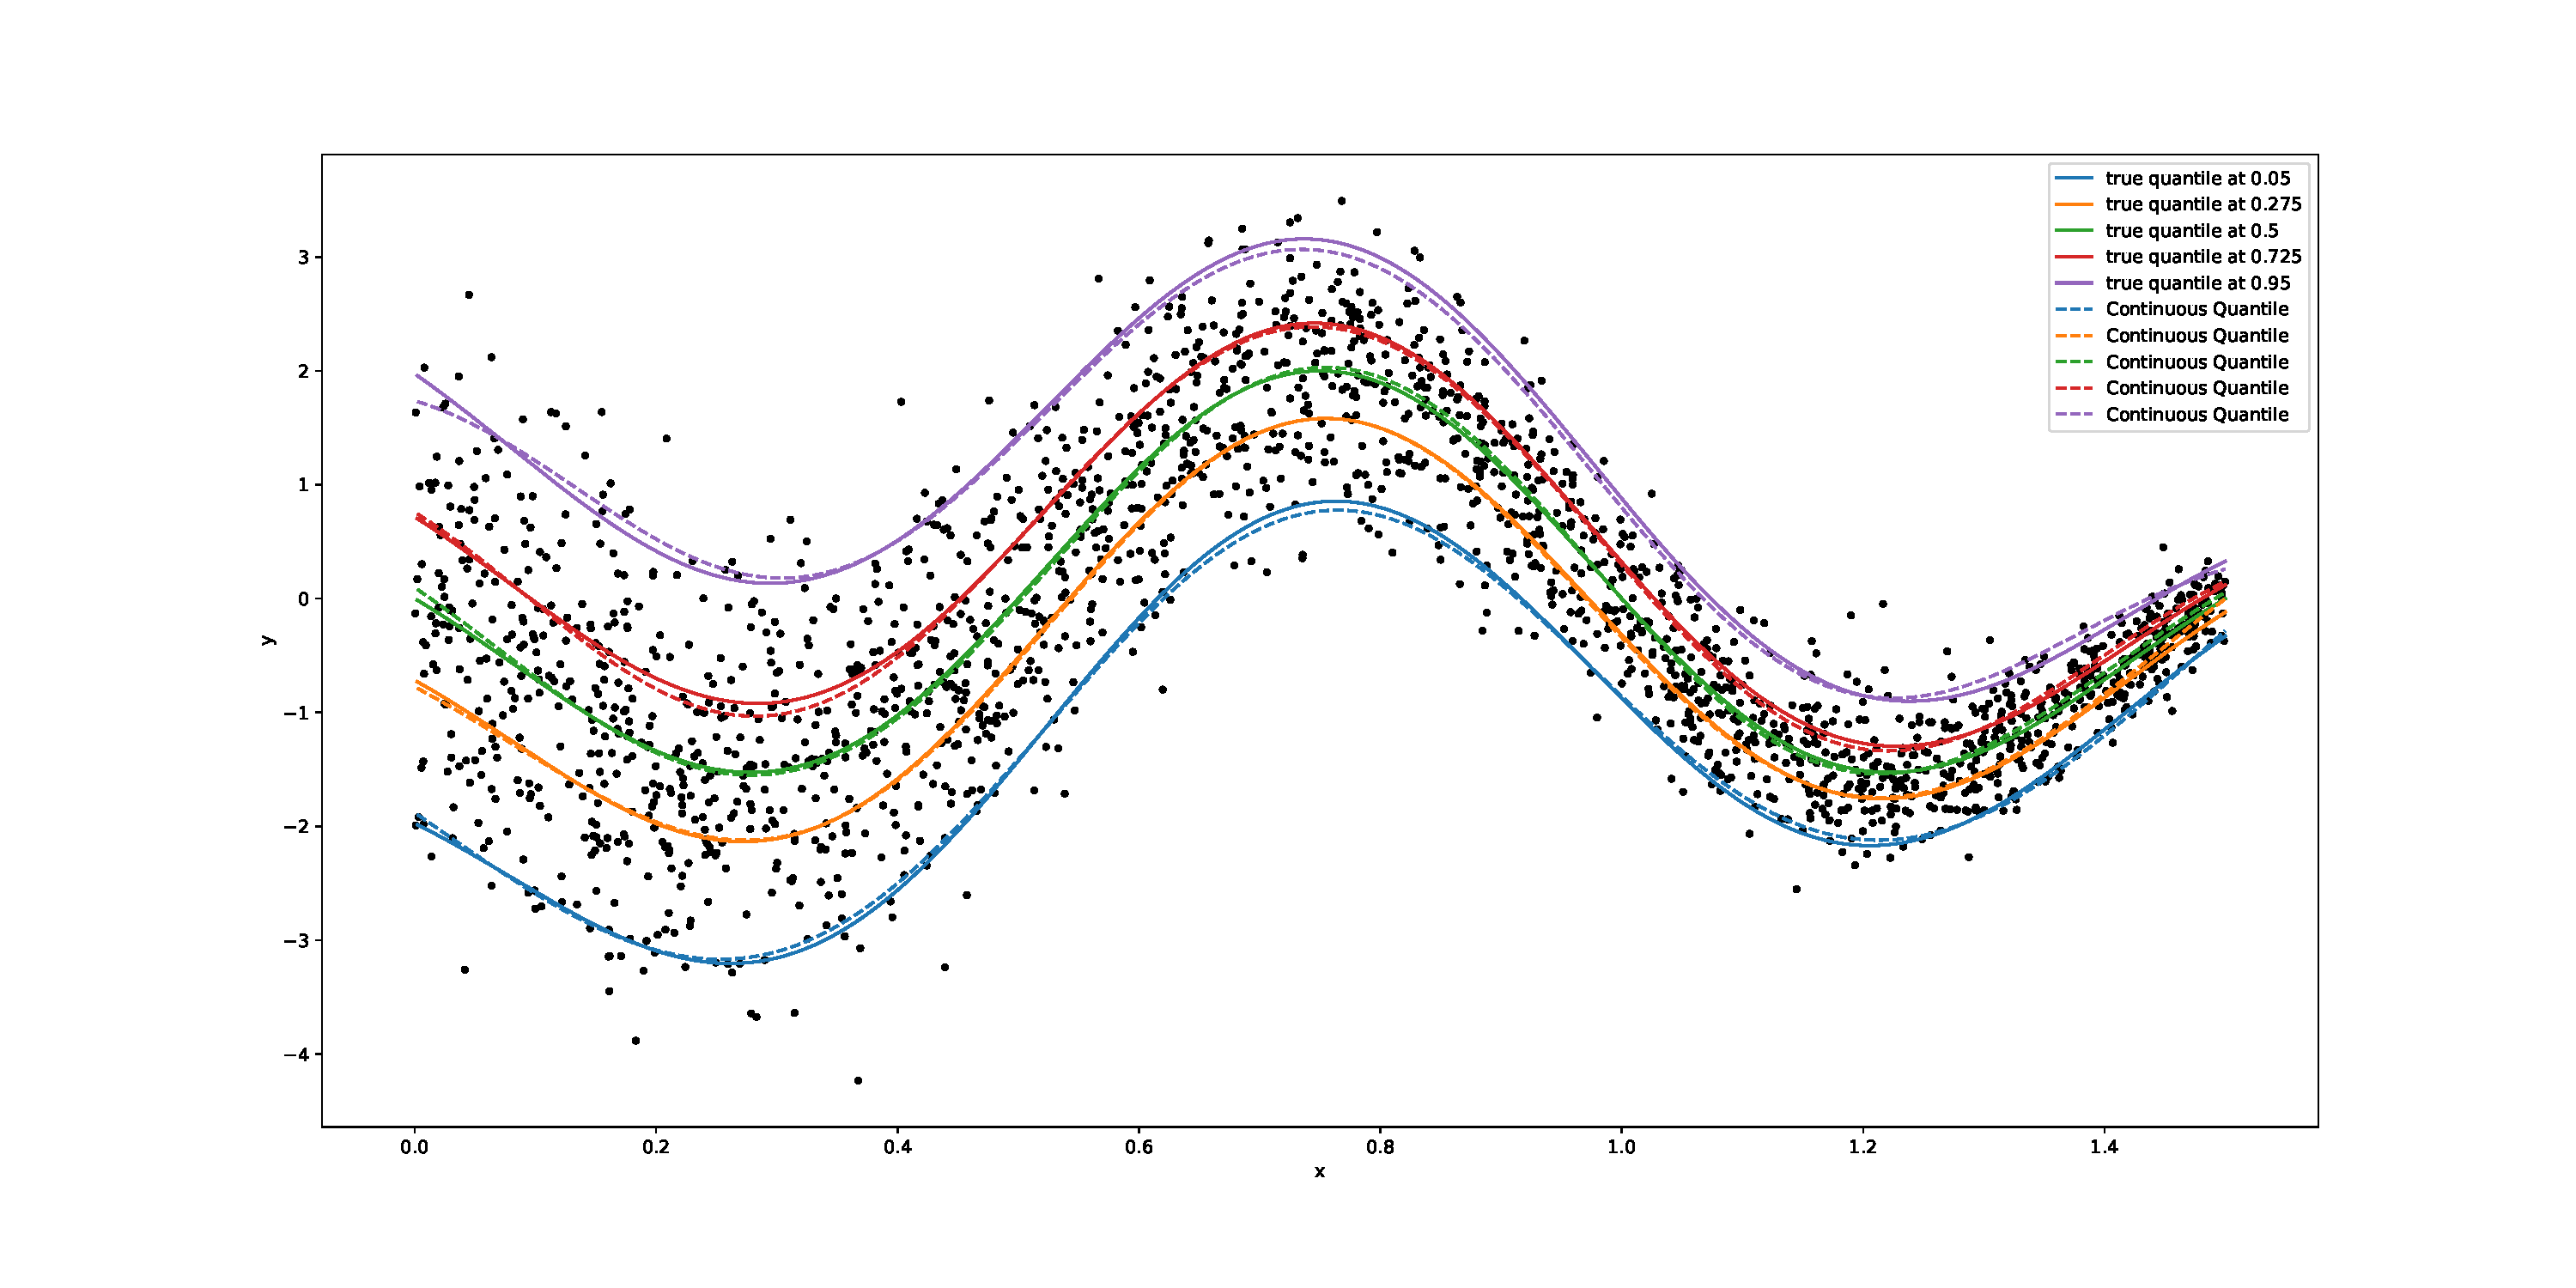
\includegraphics{./gfx/quantile_orff.pdf}}
        %\caption{Learning a continuous quantile function with ORFF
        %regression. \label{fig:quantile_orff}}
    %\end{figure}
    %\clearpage
    %\begin{figure}[htp]
        %\centering\resizebox{.8\textheight}{!}{%
        %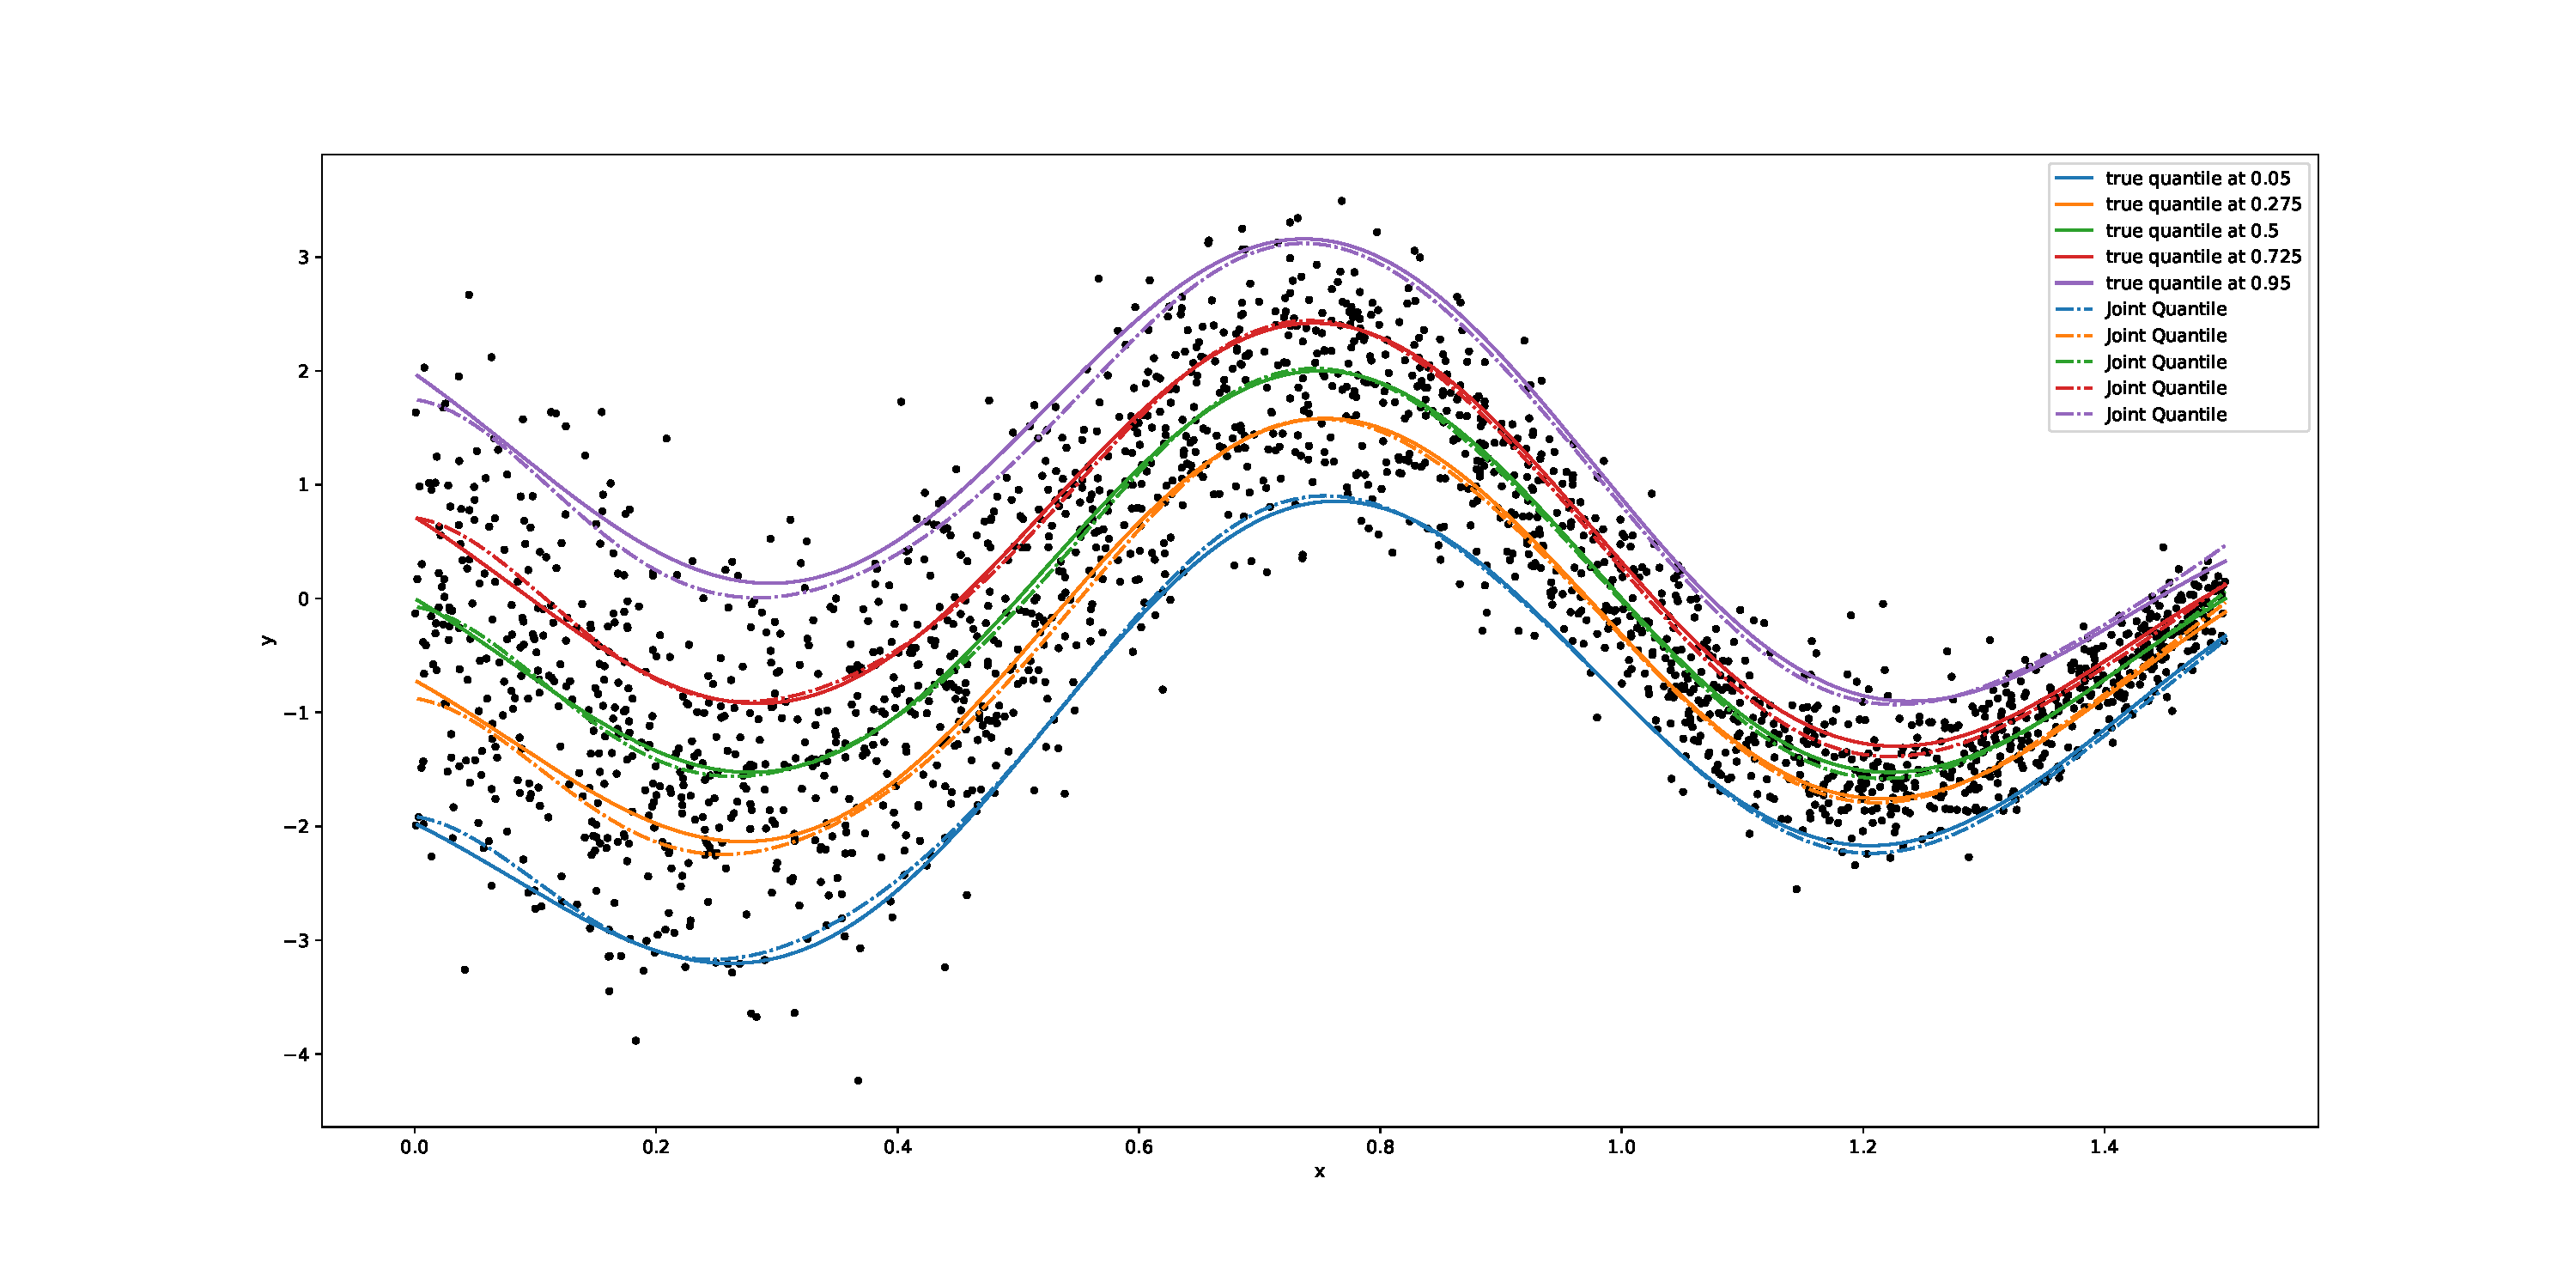
\includegraphics{./gfx/quantile_joint.pdf}}
        %\caption{Learning many quantile with joint OVK regression.
        %\label{fig:quantile_joint}}
    %\end{figure}
%\end{landscape}}
%Moreover $W^\adjoint W$ is the identity on
%$\Ima \Phi_{\tau}$ which is here $\mathcal{H}_{k_{\mathcal{T}}}$. (see the
%proof of \cref{pr:feature_operator} and \citet{Carmeli2010}). Thus we can
%choose $\Phi_\tau=\Phi(\tau)$ to be the functional Fourier feature map
%associated to $k_{\mathcal{T}}$ defined in \cref{pr:fourier_feature_map}.  Then
%we have $BB^\adjoint = I_{\mathcal{H}_{k_{\mathcal{T}}}} = W^\adjoint W$.  Thus
%we can choose $B^\adjoint = W = \Phi(\cdot)^\adjoint$ and the approximate
%feature map reads
%\begin{dmath*}
    %\tildePhi{\omega}(x)\in \mathcal{L}\left(\mathcal{H}_{k_{\mathcal{T}}};
    %\Vect_{j=1}^D L^2\left(\dual{\mathcal{T}},
    %\probability_{\dual{\Haar},\rho}\right)\right)
%\end{dmath*}
%and
%\begin{dmath*}
    %(\tildePhi{\omega}(x)g)(\tau) = \frac{1}{\sqrt{D}}\Vect_{j=1}^D
    %\begin{pmatrix}
        %\cos(x \omega_j) \Phi(\tau)^\adjoint g \\
        %\sin(x \omega_j) \Phi(\tau)^\adjoint g
    %\end{pmatrix} \condition{$\omega_j \sim \FT{k_{\mathcal{X}}}$
    %\ac{iid}}
%\end{dmath*}
%Then as proposed in \cref{ch:operator-valued_random_fourier_features} we can
%Monte-Carlo sample the functional feature map $\Phi(\tau)$ and obtain the
%\acs{ORFF} map
%\begin{dmath*}
    %\left(\widetilde{\tildePhi{\omega}}(x)g\right)(\tau) =
    %\frac{1}{\sqrt{DD'}}\Vect_{j=1}^D
    %\begin{pmatrix}
        %\cos(x \omega_j) \sum_{k=1}^{D'}
        %\left(\cos(\tau \omega_k') + \sin(\tau \omega_k')\right)g(\omega_k') \\
        %\sin(x \omega_j) \sum_{k=1}^{D'}
        %\left(\cos(\tau \omega_k') + \sin(\tau \omega_k')\right)g(\omega_k')
    %\end{pmatrix} \condition{$\omega_j \sim \FT{k_{\mathcal{X}}}$
    %\acs{iid} and $\omega_k'\sim \FT{k_{\mathcal{T}}}$ \acs{iid}.}
%\end{dmath*}
%where $g\in L^2\left(\dual{\mathcal{T}}, \probability_{\dual{\Haar},
%\rho}\right)$ and $\tau\in\mathbb{R}$. If we note
%\begin{dmath*}
    %G =
    %\begin{pmatrix}
        %g(\omega_1') & \dots & g(\omega_{D'}')
    %\end{pmatrix}^\adjoint \hiderel{\in} \mathbb{R}^{D'}
%\end{dmath*}
%we can define
%\begin{dmath*}
    %\left(\widetilde{\tildePhi{\omega}}(x)G\right)(\tau) =
    %\frac{1}{\sqrt{DD'}}\Vect_{j=1}^D
    %\begin{pmatrix}
        %\cos(x \omega_j) \sum_{k=1}^{D'}
        %\left(\cos(\tau \omega_k') + \sin(\tau \omega_k')\right)G_k \\
        %\sin(x \omega_j) \sum_{k=1}^{D'}
        %\left(\cos(\tau \omega_k') + \sin(\tau \omega_k')\right)G_k
    %\end{pmatrix} \condition{$\omega_j \sim \FT{k_{\mathcal{X}}}$
    %\acs{iid} and $\omega_k'\sim \FT{k_{\mathcal{T}}}$ \acs{iid}.}
%\end{dmath*}
%Then it is easy to verify that the adjoint operator is given by
%\begin{dmath*}
    %\left(\widetilde{\tildePhi{\omega}}(x)^\adjoint \theta\right)(\tau) =
    %\frac{1}{\sqrt{DD'}} \sum_{j=1}^D \left(\cos(x\omega_j) +
    %\sin(x\omega_j)\right) \left(\Vect_{k=1}^{D'}
    %\begin{pmatrix}
        %\cos(\tau \omega_k') \\
        %\sin(\tau \omega_k')
    %\end{pmatrix}\right)^\adjoint \theta_j
    %= \frac{1}{\sqrt{DD'}} \sum_{j=1}^D \left(\cos(x\omega_j) +
    %\sin(x\omega_j)\right) \theta_{jk} \left( \cos(\tau \omega_k') + \sin(\tau
    %\omega_k')\right)
    %\condition{$\omega_j \sim \FT{k_{\mathcal{X}}}$
    %\acs{iid} and $\omega_k'\sim \FT{k_{\mathcal{T}}}$ \acs{iid}.}
%\end{dmath*}
%where $\theta_k\in\mathbb{R}^{D'}$, for all $k \in \mathbb{N}^*_D$ and
%$\theta_{jk}\in\mathbb{R}$ for all $j \in \mathbb{N}^*_D$ and all $k \in
%\mathbb{N}^*_{D'}$. The above equations can be rewritten in matrix form which
%results in the following conjecture.
%\begin{conjecture}
    %\label{cj:functional_orff}
    %If $\tildephi{\omega}_{\mathcal{X}}$ is an \acs{RFF} for
    %$\widetilde{k}_{\mathcal{X}}$ such that
    %$\tildephi{\omega}(x)\in\mathbb{R}^D$ and $\tildephi{\omega}_{\mathcal{T}}$
    %is an \acs{RFF} for $\widetilde{k}_{\mathcal{T}}$, such that
    %$\tildephi{\omega}(\tau)\in\mathbb{R}^{D'}$ then an \acs{ORFF} map for
    %\begin{dmath*}
        %K(x, z) = k_{\mathcal{X}}(x, z) I_{\mathcal{H}_{k_{\mathcal{T}}}}
    %\end{dmath*}
    %is given for all $x\in\mathbb{R}$, all $\tau\in\mathbb{R}$ and all
    %$\Theta\in\mathcal{M}_{D,D'}(\mathbb{R})$ by
    %\begin{dmath*}
        %\left(\tildePhi{\omega}_K(x)^\adjoint \Theta \right)(\tau) =
        %\tildephi{\omega}_{\mathcal{X}}(x)^\adjoint \Theta
        %\tildephi{\omega}_{\mathcal{T}}(\tau)
    %\end{dmath*}
    %and
    %\begin{dmath*}
        %\left(\tildePhi{\omega}_K(x) G\right)(\tau) =
        %\tildephi{\omega}_{\mathcal{X}}(x)
        %\tildephi{\omega}_{\mathcal{T}}(\tau)^\adjoint G,
    %\end{dmath*}
    %where $g\in\mathbb{R}^{D'}$.
    %%but more intestingly, given $y\in\mathbb{R}$,
    %%\begin{dmath*}
        %%\tildePhi{\omega}_K(x, \tau)^\adjoint y =
        %%y \tildephi{\omega}_{\mathcal{X}}(x)
        %%\tildephi{\omega}_{\mathcal{T}}(\tau)^\adjoint.
    %%\end{dmath*}
%\end{conjecture}
%Moreover if one defines $\tildePhi{\omega}_K(x,
%\tau) = \left(\tildePhi{\omega}_K(x)^\adjoint \Theta \right)(\tau)$ one
%have of course
%\begin{dmath*}
    %\tildePhi{\omega}_K(x, \tau)^\adjoint \Theta =
    %\tildephi{\omega}_{\mathcal{X}}(x)^\adjoint \Theta
    %\tildephi{\omega}_{\mathcal{T}}(\tau)
%\end{dmath*}
%\subsection{Many quantile regression}
%From the loss defined in \cref{eq:loss_pinball} we defined the regularized risk
%using the \say{continuous} pinball loss for the quantile regression problem.
%For all $f\in\mathcal{H}_K$,
%\begin{dmath*}
    %J_{\lambda}(f) =
    %\frac{1}{N}\sum_{i=1}^N\int_{[0,1]}\left(
    %\begin{cases}
        %\tau\left(f_{x_i}(\tau) - y_i\right) & \text{if } f_{x_i}(\tau) \ge y_i
        %\\
        %(1 - \tau)\left(y_i - f_{x_i}(\tau)\right) & \text{otherwise}
    %\end{cases} \right)+ \lambda
    %\norm{f}_K^2.
%\end{dmath*}
%The issue with the above risk is that the different quantile for a given point
%$x\in\mathbb{R}$ may cross \citet{sangnier2016joint}. To avoid this to happen
%we need to force the function $f_x(\tau)$ to be \emph{increasing} in $\tau$ for
%any $x\in\mathbb{R}$.  Because a decreasing function has a negative derivative
%we can add a penalty term to the risk to avoid $f_x(\tau)$ to be decreasing in
%$\tau$.
%\begin{dmath*}
    %\Omega_{cross}(f) = - \min\left(\frac{\partial
    %f_{x_i}}{\partial\tau}(\tau),
    %0\right)
%\end{dmath*}
%Thus the regularized risk with the no crossing constraint is
%\begin{dmath*}
    %J_{\lambda_1, \lambda_2}(f) =
    %\frac{1}{N}\sum_{i=1}^N\int_{[0,1]}\left(
    %\begin{cases}
        %\tau \left(f_{x_i}(\tau) - y_i\right) & \text{if } f_{x_i}(\tau) \ge
        %y_i \\
        %(1 - \tau)\left(y_i - f_{x_i}(\tau)\right) & \text{otherwise}
    %\end{cases} -
    %\lambda_1 \min\left(\frac{\partial f_{x_i}}{\partial\tau}(\tau), 0\right)
    %\right)+ \lambda_2 \norm{f}_K^2.
%\end{dmath*}
%Eventually we replace the integral by a Monte-Carlo sampling with the uniform
%law $\mathcal{U}([0, 1])$ and plug in the approximate function of $f$ using the
%\acs{ORFF} map proposed in \cref{cj:functional_orff}. The final optimzation
%problem reads
%\begin{dmath*}
    %J_{\lambda_1, \lambda_2}(\Theta) =
    %\frac{1}{NT}\sum_{i=1}^N\sum_{t=1}^T\left(
    %\begin{cases} \tau_t
        %\left(\widetilde{f}_{x_i}(\tau_t) - y_i\right) & \text{if }
        %\widetilde{f}_{x_i}(\tau_t) \ge y_i \\
        %(1 - \tau_t)\left(y_i - f_{x_i}(\tau_t)\right) & \text{otherwise}
    %\end{cases} - \lambda_1
    %\min\left(\frac{\partial \widetilde{f}_{x_i}}{\partial\tau}(\tau_t),
    %0\right) \right)+ \lambda_2 \norm{\Theta}_{fro}^2.
%\end{dmath*}
%where $\widetilde{f}_{x}(\tau)=\tildephi{\omega}_{\mathcal{X}}(x)^\adjoint
%\Theta \tildephi{\omega}_{\mathcal{T}}(\tau)$, $\tau_t \sim \mathcal{U}([0,
%1])$ and
%\begin{dmath*}
    %\frac{\partial \widetilde{f}_{x}}{\partial\tau}(\tau)
    %= \tildephi{\omega}_{\mathcal{X}}(x)^\adjoint \Theta \frac{\partial
    %\tildephi{\omega}_{\mathcal{T}}}{\partial \tau}(\tau)
    %= \tildephi{\omega}_{\mathcal{X}}(x)^\adjoint \Theta \Vect_{k=1}^{D'}
    %\begin{pmatrix}
        %-\omega_k' \sin(\omega_k' x) \\
         %\omega_k' \cos(\omega_k' x)
    %\end{pmatrix} \condition{$\omega_k' \sim \FT{k_{\mathcal{T}}}$ \acs{iid}.}
%\end{dmath*}
%\subsubsection{Some results}
%We minimize the quantity $J_{\lambda_1, \lambda_2}(\Theta)$ on a toy dataset: a
%sine wave with some heteroscedastic noise. First we compare our methodology to
%the joint quantile regression proposed in \citet{sangnier2016joint}. We
%generate $N=2500$ for the train set and $N'=1000$ points for the test set and
%use a gaussian kernel for both $k_{\mathcal{X}}$ and $k_{\mathcal{T}}$. We
%choosed $\sigma_{\mathcal{X}} = 0.25$ and $\sigma_{\mathcal{T}}$ is set to be
%the median of the pairwise distance of the $\tau_t$'s drawn randomly from
%$\mathcal{U}([0, 1])$. Notice that $J_{\lambda_1, \lambda_2}(\Theta)$ is convex
%in $\Theta$. To avoid computing complex gradients and by lack of time, we used
%Tensorflow \citep{abadi2016tensorflow} to perform a gradient descent (with
%RMSProp \citep{tieleman2012lecture}) with automatic symbolic differentiation.
%\Cref{fig:quantile_orff} show the result for the quantile at $0.05$, $0.275$,
%$0.5$, $0.775$ and $0.95$ using the \acs{ORFF} methodology.
%\afterpage{%
%\begin{landscape}
    %\begin{figure}[htp]
        %\centering
        %\resizebox{.8\textheight}{!}{%
        %\includegraphics{./gfx/quantile_continuous.pgf}}
        %\caption{Learning a continuous quantile function with ORFF
        %regression. \label{fig:quantile_continuous}}
    %\end{figure}
%\end{landscape}}
%\Cref{fig:quantile_joint} shows the joint quantile regression of
%\citet{sangnier2016joint} on the same dataset. Not only our method matches the
%the performances of \citet{sangnier2016joint}\footnote{We reported an error
%computed with the pinball loss on the test set of $0.818$ for our method and
%$0.817$ for joint regression (note that we don't report here an average on many
%experiments to avoid randomness introduced by the random features, but the
%results seems robut in practice.)} but we cut down the computation time from
%circa $1330$ seconds to circa $30$ seconds (training and testing).  Moreover on
%contrary to \citet{sangnier2016joint} we have access to all the quantile of the
%model (see \cref{fig:quantile_continuous}).

%\subsection{One class SVM revisited}
%We also propose an extension of the celebrated \acf{OCSVM} so that it
%possible to learn jointly all the level sets.  One-class classification, also
%known as unary classification, tries to identify objects of a specific class
%amongst all objects, by learning from a training set containing only the
%objects of that class.  In this framework, we assume that we only observe
%examples of one class (referred to as the inlier class).  The second class is
%called outlier class.  We turn our attention to the \acs{OCSVM}
%of \citet{Scholkopf2001} which extends the \ac{SVM} methodology
%\citep{Cortes1995,Shawe2004} to handle training using only inliers.
%\paragraph{}
%We recall that given an hyperparameter $\nu\in [0,1]$ that controls the
%proportion of inlier, given as scalar kernel $k$, the \acs{OCSVM} problem reads
%\begin{dmath*}
    %\argmin_{f\in\mathcal{H}_k, \tau \in \mathbb{R}} \frac{1}{2}
    %\norm{f}_{\mathcal{H}_k}^2 - \nu \tau + \frac{1}{N} \sum_{i=1}^N \max(\tau
    %- f(x_i), 0)
%\end{dmath*}
%The decision function is then
%\begin{dmath*}
    %h(x, \tau) = \mathds{1}_{[\tau, \infty)}\left( f(x) \right).
%\end{dmath*}
%As in \cref{subsec:quantile_regression} we can rewrite the optimization problem
%as an integral over all the value of $\nu$ and suppose that $f$ is
%function-valued (a function of $\nu$). Moreover $\tau$ must also change its
%value according to $\mu$. Thus given a kernel $k_{\mathcal{X}}$ on the inputs
%$x\in\mathbb{R}^d$ with its approximate feature map
%$\tildephi{\omega}_{\mathcal{X}}$ and a kernel $k_{\mathcal{T}}$ on the level
%sets with its approximate feature map $\tildephi{\omega}_{\mathcal{T}}$, we
%define the continuous one-class SVM problem as
%\begin{dmath*}
    %\argmin_{f
    %\in\mathcal{H}_K,\tau\in\mathcal{H}_{k_{\mathcal{\tau}}}}\frac{1}{N}
    %\sum_{i=1}^N\int_{[0,1]}\max\left(0, \tau(\nu) - f_{x_i}(\nu)\right)d\nu +
    %\frac{1}{2}\int_{[0,1]}\nu
    %\norm{f_{\cdot}(\nu)}_{\mathcal{H}_{k_{\mathcal{X}}}}^2d\nu -
    %\int_{[0,1]}\nu\tau(\nu)d\nu.
%\end{dmath*}
%Again we can compute the integral by Monte-Carlo sampling and replace $f$ and
%$\tau$ by their respective approximation. Notice that the \acs{RKHS} of $\tau$
%should match the \acs{RKHS} of the output space of $f_K$. Hence
%\begin{dmath*}
    %\argmin_{\Theta
    %\in\mathcal{M}_{D, D'}(\mathbb{R}),\tau\in\mathbb{R}^D}\frac{1}{NT}
    %\sum_{i=1}^N\sum_{t=1}^T\max\left(0, \widetilde{\tau}(\nu_t) -
    %\widetilde{f}_{x_i}(\nu_t)\right) + \frac{1}{2T}\sum_{t=1}^T\nu_t
    %\norm{\widetilde{f}_{\cdot}(\nu_t)}_{2}^2 -
    %\frac{1}{T}\sum_{t=1}^T\nu_t\widetilde{\tau}(\nu_t),
%\end{dmath*}
%where $\nu_t \sim \mathcal{U}([0, 1])$ \acs{iid}, $\widetilde{\tau}(\nu) =
%\tildephi{\omega}_{\mathcal{T}}(\nu)$ and $\widetilde{f}_x(\nu) =
%\tildephi{\omega}(x)^\adjoint \Theta \tildephi{\omega}_{\mathcal{T}}(\nu)$. We
%also deduce that $\widetilde{f}_{\cdot}(\nu) = \Theta
%\tildephi{\omega}_{\mathcal{T}}(\nu)$. Here the natural decision function is
%\begin{dmath}
    %\label{eq:continuous_decision}
    %h(x, \nu) = \mathds{1}_{\left[\widetilde{\tau}(\nu),\infty\right)}
    %\left(\widetilde{f}_x(\nu)\right).
%\end{dmath}
%\begin{figure}
    %{\centering
    %\resizebox{2\textwidth}{!}{%% Creator: Matplotlib, PGF backend
%%
%% To include the figure in your LaTeX document, write
%%   \input{<filename>.pgf}
%%
%% Make sure the required packages are loaded in your preamble
%%   \usepackage{pgf}
%%
%% Figures using additional raster images can only be included by \input if
%% they are in the same directory as the main LaTeX file. For loading figures
%% from other directories you can use the `import` package
%%   \usepackage{import}
%% and then include the figures with
%%   \import{<path to file>}{<filename>.pgf}
%%
%% Matplotlib used the following preamble
%%   \usepackage{fontspec}
%%   \setmainfont{Times New Roman}
%%   \setsansfont{Lucida Grande}
%%   \setmonofont{Andale Mono}
%%
\begingroup%
\makeatletter%
\begin{pgfpicture}%
\pgfpathrectangle{\pgfpointorigin}{\pgfqpoint{16.000000in}{5.000000in}}%
\pgfusepath{use as bounding box, clip}%
\begin{pgfscope}%
\pgfsetbuttcap%
\pgfsetmiterjoin%
\definecolor{currentfill}{rgb}{1.000000,1.000000,1.000000}%
\pgfsetfillcolor{currentfill}%
\pgfsetlinewidth{0.000000pt}%
\definecolor{currentstroke}{rgb}{1.000000,1.000000,1.000000}%
\pgfsetstrokecolor{currentstroke}%
\pgfsetdash{}{0pt}%
\pgfpathmoveto{\pgfqpoint{0.000000in}{0.000000in}}%
\pgfpathlineto{\pgfqpoint{16.000000in}{0.000000in}}%
\pgfpathlineto{\pgfqpoint{16.000000in}{5.000000in}}%
\pgfpathlineto{\pgfqpoint{0.000000in}{5.000000in}}%
\pgfpathclose%
\pgfusepath{fill}%
\end{pgfscope}%
\begin{pgfscope}%
\pgfsetbuttcap%
\pgfsetmiterjoin%
\definecolor{currentfill}{rgb}{1.000000,1.000000,1.000000}%
\pgfsetfillcolor{currentfill}%
\pgfsetlinewidth{0.000000pt}%
\definecolor{currentstroke}{rgb}{0.000000,0.000000,0.000000}%
\pgfsetstrokecolor{currentstroke}%
\pgfsetstrokeopacity{0.000000}%
\pgfsetdash{}{0pt}%
\pgfpathmoveto{\pgfqpoint{0.663889in}{0.580556in}}%
\pgfpathlineto{\pgfqpoint{8.157639in}{0.580556in}}%
\pgfpathlineto{\pgfqpoint{8.157639in}{4.801389in}}%
\pgfpathlineto{\pgfqpoint{0.663889in}{4.801389in}}%
\pgfpathclose%
\pgfusepath{fill}%
\end{pgfscope}%
\begin{pgfscope}%
\pgfsetbuttcap%
\pgfsetroundjoin%
\definecolor{currentfill}{rgb}{0.000000,0.000000,0.000000}%
\pgfsetfillcolor{currentfill}%
\pgfsetlinewidth{0.803000pt}%
\definecolor{currentstroke}{rgb}{0.000000,0.000000,0.000000}%
\pgfsetstrokecolor{currentstroke}%
\pgfsetdash{}{0pt}%
\pgfsys@defobject{currentmarker}{\pgfqpoint{0.000000in}{-0.048611in}}{\pgfqpoint{0.000000in}{0.000000in}}{%
\pgfpathmoveto{\pgfqpoint{0.000000in}{0.000000in}}%
\pgfpathlineto{\pgfqpoint{0.000000in}{-0.048611in}}%
\pgfusepath{stroke,fill}%
}%
\begin{pgfscope}%
\pgfsys@transformshift{1.004514in}{0.580556in}%
\pgfsys@useobject{currentmarker}{}%
\end{pgfscope}%
\end{pgfscope}%
\begin{pgfscope}%
\pgftext[x=1.004514in,y=0.483333in,,top]{\sffamily\fontsize{10.000000}{12.000000}\selectfont 0.0}%
\end{pgfscope}%
\begin{pgfscope}%
\pgfsetbuttcap%
\pgfsetroundjoin%
\definecolor{currentfill}{rgb}{0.000000,0.000000,0.000000}%
\pgfsetfillcolor{currentfill}%
\pgfsetlinewidth{0.803000pt}%
\definecolor{currentstroke}{rgb}{0.000000,0.000000,0.000000}%
\pgfsetstrokecolor{currentstroke}%
\pgfsetdash{}{0pt}%
\pgfsys@defobject{currentmarker}{\pgfqpoint{0.000000in}{-0.048611in}}{\pgfqpoint{0.000000in}{0.000000in}}{%
\pgfpathmoveto{\pgfqpoint{0.000000in}{0.000000in}}%
\pgfpathlineto{\pgfqpoint{0.000000in}{-0.048611in}}%
\pgfusepath{stroke,fill}%
}%
\begin{pgfscope}%
\pgfsys@transformshift{2.367014in}{0.580556in}%
\pgfsys@useobject{currentmarker}{}%
\end{pgfscope}%
\end{pgfscope}%
\begin{pgfscope}%
\pgftext[x=2.367014in,y=0.483333in,,top]{\sffamily\fontsize{10.000000}{12.000000}\selectfont 0.2}%
\end{pgfscope}%
\begin{pgfscope}%
\pgfsetbuttcap%
\pgfsetroundjoin%
\definecolor{currentfill}{rgb}{0.000000,0.000000,0.000000}%
\pgfsetfillcolor{currentfill}%
\pgfsetlinewidth{0.803000pt}%
\definecolor{currentstroke}{rgb}{0.000000,0.000000,0.000000}%
\pgfsetstrokecolor{currentstroke}%
\pgfsetdash{}{0pt}%
\pgfsys@defobject{currentmarker}{\pgfqpoint{0.000000in}{-0.048611in}}{\pgfqpoint{0.000000in}{0.000000in}}{%
\pgfpathmoveto{\pgfqpoint{0.000000in}{0.000000in}}%
\pgfpathlineto{\pgfqpoint{0.000000in}{-0.048611in}}%
\pgfusepath{stroke,fill}%
}%
\begin{pgfscope}%
\pgfsys@transformshift{3.729514in}{0.580556in}%
\pgfsys@useobject{currentmarker}{}%
\end{pgfscope}%
\end{pgfscope}%
\begin{pgfscope}%
\pgftext[x=3.729514in,y=0.483333in,,top]{\sffamily\fontsize{10.000000}{12.000000}\selectfont 0.4}%
\end{pgfscope}%
\begin{pgfscope}%
\pgfsetbuttcap%
\pgfsetroundjoin%
\definecolor{currentfill}{rgb}{0.000000,0.000000,0.000000}%
\pgfsetfillcolor{currentfill}%
\pgfsetlinewidth{0.803000pt}%
\definecolor{currentstroke}{rgb}{0.000000,0.000000,0.000000}%
\pgfsetstrokecolor{currentstroke}%
\pgfsetdash{}{0pt}%
\pgfsys@defobject{currentmarker}{\pgfqpoint{0.000000in}{-0.048611in}}{\pgfqpoint{0.000000in}{0.000000in}}{%
\pgfpathmoveto{\pgfqpoint{0.000000in}{0.000000in}}%
\pgfpathlineto{\pgfqpoint{0.000000in}{-0.048611in}}%
\pgfusepath{stroke,fill}%
}%
\begin{pgfscope}%
\pgfsys@transformshift{5.092014in}{0.580556in}%
\pgfsys@useobject{currentmarker}{}%
\end{pgfscope}%
\end{pgfscope}%
\begin{pgfscope}%
\pgftext[x=5.092014in,y=0.483333in,,top]{\sffamily\fontsize{10.000000}{12.000000}\selectfont 0.6}%
\end{pgfscope}%
\begin{pgfscope}%
\pgfsetbuttcap%
\pgfsetroundjoin%
\definecolor{currentfill}{rgb}{0.000000,0.000000,0.000000}%
\pgfsetfillcolor{currentfill}%
\pgfsetlinewidth{0.803000pt}%
\definecolor{currentstroke}{rgb}{0.000000,0.000000,0.000000}%
\pgfsetstrokecolor{currentstroke}%
\pgfsetdash{}{0pt}%
\pgfsys@defobject{currentmarker}{\pgfqpoint{0.000000in}{-0.048611in}}{\pgfqpoint{0.000000in}{0.000000in}}{%
\pgfpathmoveto{\pgfqpoint{0.000000in}{0.000000in}}%
\pgfpathlineto{\pgfqpoint{0.000000in}{-0.048611in}}%
\pgfusepath{stroke,fill}%
}%
\begin{pgfscope}%
\pgfsys@transformshift{6.454514in}{0.580556in}%
\pgfsys@useobject{currentmarker}{}%
\end{pgfscope}%
\end{pgfscope}%
\begin{pgfscope}%
\pgftext[x=6.454514in,y=0.483333in,,top]{\sffamily\fontsize{10.000000}{12.000000}\selectfont 0.8}%
\end{pgfscope}%
\begin{pgfscope}%
\pgfsetbuttcap%
\pgfsetroundjoin%
\definecolor{currentfill}{rgb}{0.000000,0.000000,0.000000}%
\pgfsetfillcolor{currentfill}%
\pgfsetlinewidth{0.803000pt}%
\definecolor{currentstroke}{rgb}{0.000000,0.000000,0.000000}%
\pgfsetstrokecolor{currentstroke}%
\pgfsetdash{}{0pt}%
\pgfsys@defobject{currentmarker}{\pgfqpoint{0.000000in}{-0.048611in}}{\pgfqpoint{0.000000in}{0.000000in}}{%
\pgfpathmoveto{\pgfqpoint{0.000000in}{0.000000in}}%
\pgfpathlineto{\pgfqpoint{0.000000in}{-0.048611in}}%
\pgfusepath{stroke,fill}%
}%
\begin{pgfscope}%
\pgfsys@transformshift{7.817014in}{0.580556in}%
\pgfsys@useobject{currentmarker}{}%
\end{pgfscope}%
\end{pgfscope}%
\begin{pgfscope}%
\pgftext[x=7.817014in,y=0.483333in,,top]{\sffamily\fontsize{10.000000}{12.000000}\selectfont 1.0}%
\end{pgfscope}%
\begin{pgfscope}%
\pgftext[x=4.410764in,y=0.293908in,,top]{\sffamily\fontsize{10.000000}{12.000000}\selectfont \(\displaystyle \nu\)}%
\end{pgfscope}%
\begin{pgfscope}%
\pgfsetbuttcap%
\pgfsetroundjoin%
\definecolor{currentfill}{rgb}{0.000000,0.000000,0.000000}%
\pgfsetfillcolor{currentfill}%
\pgfsetlinewidth{0.803000pt}%
\definecolor{currentstroke}{rgb}{0.000000,0.000000,0.000000}%
\pgfsetstrokecolor{currentstroke}%
\pgfsetdash{}{0pt}%
\pgfsys@defobject{currentmarker}{\pgfqpoint{-0.048611in}{0.000000in}}{\pgfqpoint{0.000000in}{0.000000in}}{%
\pgfpathmoveto{\pgfqpoint{0.000000in}{0.000000in}}%
\pgfpathlineto{\pgfqpoint{-0.048611in}{0.000000in}}%
\pgfusepath{stroke,fill}%
}%
\begin{pgfscope}%
\pgfsys@transformshift{0.663889in}{0.772412in}%
\pgfsys@useobject{currentmarker}{}%
\end{pgfscope}%
\end{pgfscope}%
\begin{pgfscope}%
\pgftext[x=0.347076in,y=0.718870in,left,base]{\sffamily\fontsize{10.000000}{12.000000}\selectfont 0.0}%
\end{pgfscope}%
\begin{pgfscope}%
\pgfsetbuttcap%
\pgfsetroundjoin%
\definecolor{currentfill}{rgb}{0.000000,0.000000,0.000000}%
\pgfsetfillcolor{currentfill}%
\pgfsetlinewidth{0.803000pt}%
\definecolor{currentstroke}{rgb}{0.000000,0.000000,0.000000}%
\pgfsetstrokecolor{currentstroke}%
\pgfsetdash{}{0pt}%
\pgfsys@defobject{currentmarker}{\pgfqpoint{-0.048611in}{0.000000in}}{\pgfqpoint{0.000000in}{0.000000in}}{%
\pgfpathmoveto{\pgfqpoint{0.000000in}{0.000000in}}%
\pgfpathlineto{\pgfqpoint{-0.048611in}{0.000000in}}%
\pgfusepath{stroke,fill}%
}%
\begin{pgfscope}%
\pgfsys@transformshift{0.663889in}{1.539836in}%
\pgfsys@useobject{currentmarker}{}%
\end{pgfscope}%
\end{pgfscope}%
\begin{pgfscope}%
\pgftext[x=0.347076in,y=1.486294in,left,base]{\sffamily\fontsize{10.000000}{12.000000}\selectfont 0.2}%
\end{pgfscope}%
\begin{pgfscope}%
\pgfsetbuttcap%
\pgfsetroundjoin%
\definecolor{currentfill}{rgb}{0.000000,0.000000,0.000000}%
\pgfsetfillcolor{currentfill}%
\pgfsetlinewidth{0.803000pt}%
\definecolor{currentstroke}{rgb}{0.000000,0.000000,0.000000}%
\pgfsetstrokecolor{currentstroke}%
\pgfsetdash{}{0pt}%
\pgfsys@defobject{currentmarker}{\pgfqpoint{-0.048611in}{0.000000in}}{\pgfqpoint{0.000000in}{0.000000in}}{%
\pgfpathmoveto{\pgfqpoint{0.000000in}{0.000000in}}%
\pgfpathlineto{\pgfqpoint{-0.048611in}{0.000000in}}%
\pgfusepath{stroke,fill}%
}%
\begin{pgfscope}%
\pgfsys@transformshift{0.663889in}{2.307260in}%
\pgfsys@useobject{currentmarker}{}%
\end{pgfscope}%
\end{pgfscope}%
\begin{pgfscope}%
\pgftext[x=0.347076in,y=2.253719in,left,base]{\sffamily\fontsize{10.000000}{12.000000}\selectfont 0.4}%
\end{pgfscope}%
\begin{pgfscope}%
\pgfsetbuttcap%
\pgfsetroundjoin%
\definecolor{currentfill}{rgb}{0.000000,0.000000,0.000000}%
\pgfsetfillcolor{currentfill}%
\pgfsetlinewidth{0.803000pt}%
\definecolor{currentstroke}{rgb}{0.000000,0.000000,0.000000}%
\pgfsetstrokecolor{currentstroke}%
\pgfsetdash{}{0pt}%
\pgfsys@defobject{currentmarker}{\pgfqpoint{-0.048611in}{0.000000in}}{\pgfqpoint{0.000000in}{0.000000in}}{%
\pgfpathmoveto{\pgfqpoint{0.000000in}{0.000000in}}%
\pgfpathlineto{\pgfqpoint{-0.048611in}{0.000000in}}%
\pgfusepath{stroke,fill}%
}%
\begin{pgfscope}%
\pgfsys@transformshift{0.663889in}{3.074684in}%
\pgfsys@useobject{currentmarker}{}%
\end{pgfscope}%
\end{pgfscope}%
\begin{pgfscope}%
\pgftext[x=0.347076in,y=3.021143in,left,base]{\sffamily\fontsize{10.000000}{12.000000}\selectfont 0.6}%
\end{pgfscope}%
\begin{pgfscope}%
\pgfsetbuttcap%
\pgfsetroundjoin%
\definecolor{currentfill}{rgb}{0.000000,0.000000,0.000000}%
\pgfsetfillcolor{currentfill}%
\pgfsetlinewidth{0.803000pt}%
\definecolor{currentstroke}{rgb}{0.000000,0.000000,0.000000}%
\pgfsetstrokecolor{currentstroke}%
\pgfsetdash{}{0pt}%
\pgfsys@defobject{currentmarker}{\pgfqpoint{-0.048611in}{0.000000in}}{\pgfqpoint{0.000000in}{0.000000in}}{%
\pgfpathmoveto{\pgfqpoint{0.000000in}{0.000000in}}%
\pgfpathlineto{\pgfqpoint{-0.048611in}{0.000000in}}%
\pgfusepath{stroke,fill}%
}%
\begin{pgfscope}%
\pgfsys@transformshift{0.663889in}{3.842109in}%
\pgfsys@useobject{currentmarker}{}%
\end{pgfscope}%
\end{pgfscope}%
\begin{pgfscope}%
\pgftext[x=0.347076in,y=3.788567in,left,base]{\sffamily\fontsize{10.000000}{12.000000}\selectfont 0.8}%
\end{pgfscope}%
\begin{pgfscope}%
\pgfsetbuttcap%
\pgfsetroundjoin%
\definecolor{currentfill}{rgb}{0.000000,0.000000,0.000000}%
\pgfsetfillcolor{currentfill}%
\pgfsetlinewidth{0.803000pt}%
\definecolor{currentstroke}{rgb}{0.000000,0.000000,0.000000}%
\pgfsetstrokecolor{currentstroke}%
\pgfsetdash{}{0pt}%
\pgfsys@defobject{currentmarker}{\pgfqpoint{-0.048611in}{0.000000in}}{\pgfqpoint{0.000000in}{0.000000in}}{%
\pgfpathmoveto{\pgfqpoint{0.000000in}{0.000000in}}%
\pgfpathlineto{\pgfqpoint{-0.048611in}{0.000000in}}%
\pgfusepath{stroke,fill}%
}%
\begin{pgfscope}%
\pgfsys@transformshift{0.663889in}{4.609533in}%
\pgfsys@useobject{currentmarker}{}%
\end{pgfscope}%
\end{pgfscope}%
\begin{pgfscope}%
\pgftext[x=0.347076in,y=4.555991in,left,base]{\sffamily\fontsize{10.000000}{12.000000}\selectfont 1.0}%
\end{pgfscope}%
\begin{pgfscope}%
\pgftext[x=0.291520in,y=2.690972in,,bottom,rotate=90.000000]{\sffamily\fontsize{10.000000}{12.000000}\selectfont percentage of inliers}%
\end{pgfscope}%
\begin{pgfscope}%
\pgfpathrectangle{\pgfqpoint{0.663889in}{0.580556in}}{\pgfqpoint{7.493750in}{4.220833in}} %
\pgfusepath{clip}%
\pgfsetrectcap%
\pgfsetroundjoin%
\pgfsetlinewidth{1.505625pt}%
\definecolor{currentstroke}{rgb}{0.121569,0.466667,0.705882}%
\pgfsetstrokecolor{currentstroke}%
\pgfsetdash{}{0pt}%
\pgfpathmoveto{\pgfqpoint{1.004514in}{4.099744in}}%
\pgfpathlineto{\pgfqpoint{1.073327in}{4.181968in}}%
\pgfpathlineto{\pgfqpoint{1.142140in}{4.072336in}}%
\pgfpathlineto{\pgfqpoint{1.210953in}{4.006557in}}%
\pgfpathlineto{\pgfqpoint{1.279766in}{3.979149in}}%
\pgfpathlineto{\pgfqpoint{1.348580in}{3.973667in}}%
\pgfpathlineto{\pgfqpoint{1.417393in}{3.951741in}}%
\pgfpathlineto{\pgfqpoint{1.486206in}{3.918851in}}%
\pgfpathlineto{\pgfqpoint{1.555019in}{3.842109in}}%
\pgfpathlineto{\pgfqpoint{1.623832in}{3.820182in}}%
\pgfpathlineto{\pgfqpoint{1.692645in}{3.787293in}}%
\pgfpathlineto{\pgfqpoint{1.761458in}{3.743440in}}%
\pgfpathlineto{\pgfqpoint{1.830271in}{3.710550in}}%
\pgfpathlineto{\pgfqpoint{1.899085in}{3.672179in}}%
\pgfpathlineto{\pgfqpoint{1.967898in}{3.633808in}}%
\pgfpathlineto{\pgfqpoint{2.036711in}{3.595437in}}%
\pgfpathlineto{\pgfqpoint{2.105524in}{3.578992in}}%
\pgfpathlineto{\pgfqpoint{2.174337in}{3.557065in}}%
\pgfpathlineto{\pgfqpoint{2.243150in}{3.480323in}}%
\pgfpathlineto{\pgfqpoint{2.311963in}{3.436470in}}%
\pgfpathlineto{\pgfqpoint{2.380777in}{3.425507in}}%
\pgfpathlineto{\pgfqpoint{2.449590in}{3.398099in}}%
\pgfpathlineto{\pgfqpoint{2.518403in}{3.354246in}}%
\pgfpathlineto{\pgfqpoint{2.587216in}{3.321356in}}%
\pgfpathlineto{\pgfqpoint{2.656029in}{3.293948in}}%
\pgfpathlineto{\pgfqpoint{2.724842in}{3.272022in}}%
\pgfpathlineto{\pgfqpoint{2.793655in}{3.244614in}}%
\pgfpathlineto{\pgfqpoint{2.862468in}{3.206243in}}%
\pgfpathlineto{\pgfqpoint{2.931282in}{3.140464in}}%
\pgfpathlineto{\pgfqpoint{3.000095in}{3.107574in}}%
\pgfpathlineto{\pgfqpoint{3.068908in}{3.080166in}}%
\pgfpathlineto{\pgfqpoint{3.137721in}{3.058240in}}%
\pgfpathlineto{\pgfqpoint{3.206534in}{3.003424in}}%
\pgfpathlineto{\pgfqpoint{3.275347in}{2.970534in}}%
\pgfpathlineto{\pgfqpoint{3.344160in}{2.943126in}}%
\pgfpathlineto{\pgfqpoint{3.412973in}{2.932163in}}%
\pgfpathlineto{\pgfqpoint{3.481787in}{2.910236in}}%
\pgfpathlineto{\pgfqpoint{3.550600in}{2.860902in}}%
\pgfpathlineto{\pgfqpoint{3.619413in}{2.811567in}}%
\pgfpathlineto{\pgfqpoint{3.688226in}{2.756751in}}%
\pgfpathlineto{\pgfqpoint{3.757039in}{2.723862in}}%
\pgfpathlineto{\pgfqpoint{3.825852in}{2.712899in}}%
\pgfpathlineto{\pgfqpoint{3.894665in}{2.696454in}}%
\pgfpathlineto{\pgfqpoint{3.963479in}{2.641638in}}%
\pgfpathlineto{\pgfqpoint{4.032292in}{2.625193in}}%
\pgfpathlineto{\pgfqpoint{4.101105in}{2.575859in}}%
\pgfpathlineto{\pgfqpoint{4.169918in}{2.559414in}}%
\pgfpathlineto{\pgfqpoint{4.238731in}{2.515561in}}%
\pgfpathlineto{\pgfqpoint{4.307544in}{2.477190in}}%
\pgfpathlineto{\pgfqpoint{4.376357in}{2.416892in}}%
\pgfpathlineto{\pgfqpoint{4.445170in}{2.400447in}}%
\pgfpathlineto{\pgfqpoint{4.513984in}{2.373039in}}%
\pgfpathlineto{\pgfqpoint{4.582797in}{2.351113in}}%
\pgfpathlineto{\pgfqpoint{4.651610in}{2.323705in}}%
\pgfpathlineto{\pgfqpoint{4.720423in}{2.285334in}}%
\pgfpathlineto{\pgfqpoint{4.789236in}{2.252444in}}%
\pgfpathlineto{\pgfqpoint{4.858049in}{2.164738in}}%
\pgfpathlineto{\pgfqpoint{4.926862in}{2.137330in}}%
\pgfpathlineto{\pgfqpoint{4.995676in}{2.115404in}}%
\pgfpathlineto{\pgfqpoint{5.064489in}{2.087996in}}%
\pgfpathlineto{\pgfqpoint{5.133302in}{2.060588in}}%
\pgfpathlineto{\pgfqpoint{5.202115in}{2.044143in}}%
\pgfpathlineto{\pgfqpoint{5.270928in}{2.016735in}}%
\pgfpathlineto{\pgfqpoint{5.339741in}{1.989327in}}%
\pgfpathlineto{\pgfqpoint{5.408554in}{1.945474in}}%
\pgfpathlineto{\pgfqpoint{5.477367in}{1.923548in}}%
\pgfpathlineto{\pgfqpoint{5.546181in}{1.885177in}}%
\pgfpathlineto{\pgfqpoint{5.614994in}{1.857769in}}%
\pgfpathlineto{\pgfqpoint{5.683807in}{1.802953in}}%
\pgfpathlineto{\pgfqpoint{5.752620in}{1.759100in}}%
\pgfpathlineto{\pgfqpoint{5.821433in}{1.742655in}}%
\pgfpathlineto{\pgfqpoint{5.890246in}{1.698802in}}%
\pgfpathlineto{\pgfqpoint{5.959059in}{1.660431in}}%
\pgfpathlineto{\pgfqpoint{6.027872in}{1.638505in}}%
\pgfpathlineto{\pgfqpoint{6.096686in}{1.611097in}}%
\pgfpathlineto{\pgfqpoint{6.165499in}{1.578207in}}%
\pgfpathlineto{\pgfqpoint{6.234312in}{1.539836in}}%
\pgfpathlineto{\pgfqpoint{6.303125in}{1.490501in}}%
\pgfpathlineto{\pgfqpoint{6.371938in}{1.457612in}}%
\pgfpathlineto{\pgfqpoint{6.440751in}{1.424722in}}%
\pgfpathlineto{\pgfqpoint{6.509564in}{1.419241in}}%
\pgfpathlineto{\pgfqpoint{6.578378in}{1.386351in}}%
\pgfpathlineto{\pgfqpoint{6.647191in}{1.347980in}}%
\pgfpathlineto{\pgfqpoint{6.716004in}{1.304127in}}%
\pgfpathlineto{\pgfqpoint{6.784817in}{1.265756in}}%
\pgfpathlineto{\pgfqpoint{6.853630in}{1.249311in}}%
\pgfpathlineto{\pgfqpoint{6.922443in}{1.205458in}}%
\pgfpathlineto{\pgfqpoint{6.991256in}{1.161605in}}%
\pgfpathlineto{\pgfqpoint{7.060069in}{1.134197in}}%
\pgfpathlineto{\pgfqpoint{7.128883in}{1.095826in}}%
\pgfpathlineto{\pgfqpoint{7.197696in}{1.073900in}}%
\pgfpathlineto{\pgfqpoint{7.266509in}{1.057455in}}%
\pgfpathlineto{\pgfqpoint{7.335322in}{1.019084in}}%
\pgfpathlineto{\pgfqpoint{7.404135in}{0.980712in}}%
\pgfpathlineto{\pgfqpoint{7.472948in}{0.925896in}}%
\pgfpathlineto{\pgfqpoint{7.541761in}{0.882044in}}%
\pgfpathlineto{\pgfqpoint{7.610574in}{0.871080in}}%
\pgfpathlineto{\pgfqpoint{7.679388in}{0.843672in}}%
\pgfpathlineto{\pgfqpoint{7.748201in}{0.843672in}}%
\pgfpathlineto{\pgfqpoint{7.817014in}{0.854636in}}%
\pgfusepath{stroke}%
\end{pgfscope}%
\begin{pgfscope}%
\pgfpathrectangle{\pgfqpoint{0.663889in}{0.580556in}}{\pgfqpoint{7.493750in}{4.220833in}} %
\pgfusepath{clip}%
\pgfsetrectcap%
\pgfsetroundjoin%
\pgfsetlinewidth{1.505625pt}%
\definecolor{currentstroke}{rgb}{1.000000,0.498039,0.054902}%
\pgfsetstrokecolor{currentstroke}%
\pgfsetdash{}{0pt}%
\pgfpathmoveto{\pgfqpoint{1.004514in}{4.393923in}}%
\pgfpathlineto{\pgfqpoint{1.073327in}{4.554717in}}%
\pgfpathlineto{\pgfqpoint{1.142140in}{4.474320in}}%
\pgfpathlineto{\pgfqpoint{1.210953in}{4.448739in}}%
\pgfpathlineto{\pgfqpoint{1.279766in}{4.434122in}}%
\pgfpathlineto{\pgfqpoint{1.348580in}{4.423158in}}%
\pgfpathlineto{\pgfqpoint{1.417393in}{4.401232in}}%
\pgfpathlineto{\pgfqpoint{1.486206in}{4.377478in}}%
\pgfpathlineto{\pgfqpoint{1.555019in}{4.329971in}}%
\pgfpathlineto{\pgfqpoint{1.623832in}{4.282464in}}%
\pgfpathlineto{\pgfqpoint{1.692645in}{4.247747in}}%
\pgfpathlineto{\pgfqpoint{1.761458in}{4.203894in}}%
\pgfpathlineto{\pgfqpoint{1.830271in}{4.139942in}}%
\pgfpathlineto{\pgfqpoint{1.899085in}{4.085126in}}%
\pgfpathlineto{\pgfqpoint{1.967898in}{4.039446in}}%
\pgfpathlineto{\pgfqpoint{2.036711in}{4.008384in}}%
\pgfpathlineto{\pgfqpoint{2.105524in}{3.971840in}}%
\pgfpathlineto{\pgfqpoint{2.174337in}{3.931641in}}%
\pgfpathlineto{\pgfqpoint{2.243150in}{3.896925in}}%
\pgfpathlineto{\pgfqpoint{2.311963in}{3.864035in}}%
\pgfpathlineto{\pgfqpoint{2.380777in}{3.827491in}}%
\pgfpathlineto{\pgfqpoint{2.449590in}{3.805565in}}%
\pgfpathlineto{\pgfqpoint{2.518403in}{3.785465in}}%
\pgfpathlineto{\pgfqpoint{2.587216in}{3.758057in}}%
\pgfpathlineto{\pgfqpoint{2.656029in}{3.728822in}}%
\pgfpathlineto{\pgfqpoint{2.724842in}{3.706896in}}%
\pgfpathlineto{\pgfqpoint{2.793655in}{3.677661in}}%
\pgfpathlineto{\pgfqpoint{2.862468in}{3.626499in}}%
\pgfpathlineto{\pgfqpoint{2.931282in}{3.591782in}}%
\pgfpathlineto{\pgfqpoint{3.000095in}{3.562547in}}%
\pgfpathlineto{\pgfqpoint{3.068908in}{3.527830in}}%
\pgfpathlineto{\pgfqpoint{3.137721in}{3.496768in}}%
\pgfpathlineto{\pgfqpoint{3.206534in}{3.480323in}}%
\pgfpathlineto{\pgfqpoint{3.275347in}{3.471187in}}%
\pgfpathlineto{\pgfqpoint{3.344160in}{3.441952in}}%
\pgfpathlineto{\pgfqpoint{3.412973in}{3.412716in}}%
\pgfpathlineto{\pgfqpoint{3.481787in}{3.378000in}}%
\pgfpathlineto{\pgfqpoint{3.550600in}{3.337801in}}%
\pgfpathlineto{\pgfqpoint{3.619413in}{3.303084in}}%
\pgfpathlineto{\pgfqpoint{3.688226in}{3.257404in}}%
\pgfpathlineto{\pgfqpoint{3.757039in}{3.200761in}}%
\pgfpathlineto{\pgfqpoint{3.825852in}{3.156908in}}%
\pgfpathlineto{\pgfqpoint{3.894665in}{3.118537in}}%
\pgfpathlineto{\pgfqpoint{3.963479in}{3.089302in}}%
\pgfpathlineto{\pgfqpoint{4.032292in}{3.063721in}}%
\pgfpathlineto{\pgfqpoint{4.101105in}{3.023523in}}%
\pgfpathlineto{\pgfqpoint{4.169918in}{2.977843in}}%
\pgfpathlineto{\pgfqpoint{4.238731in}{2.935817in}}%
\pgfpathlineto{\pgfqpoint{4.307544in}{2.884655in}}%
\pgfpathlineto{\pgfqpoint{4.376357in}{2.818876in}}%
\pgfpathlineto{\pgfqpoint{4.445170in}{2.780505in}}%
\pgfpathlineto{\pgfqpoint{4.513984in}{2.723862in}}%
\pgfpathlineto{\pgfqpoint{4.582797in}{2.681836in}}%
\pgfpathlineto{\pgfqpoint{4.651610in}{2.661737in}}%
\pgfpathlineto{\pgfqpoint{4.720423in}{2.632502in}}%
\pgfpathlineto{\pgfqpoint{4.789236in}{2.603267in}}%
\pgfpathlineto{\pgfqpoint{4.858049in}{2.563068in}}%
\pgfpathlineto{\pgfqpoint{4.926862in}{2.524697in}}%
\pgfpathlineto{\pgfqpoint{4.995676in}{2.488153in}}%
\pgfpathlineto{\pgfqpoint{5.064489in}{2.440646in}}%
\pgfpathlineto{\pgfqpoint{5.133302in}{2.407756in}}%
\pgfpathlineto{\pgfqpoint{5.202115in}{2.380348in}}%
\pgfpathlineto{\pgfqpoint{5.270928in}{2.347459in}}%
\pgfpathlineto{\pgfqpoint{5.339741in}{2.292642in}}%
\pgfpathlineto{\pgfqpoint{5.408554in}{2.221382in}}%
\pgfpathlineto{\pgfqpoint{5.477367in}{2.159257in}}%
\pgfpathlineto{\pgfqpoint{5.546181in}{2.095305in}}%
\pgfpathlineto{\pgfqpoint{5.614994in}{2.038662in}}%
\pgfpathlineto{\pgfqpoint{5.683807in}{1.994809in}}%
\pgfpathlineto{\pgfqpoint{5.752620in}{1.943647in}}%
\pgfpathlineto{\pgfqpoint{5.821433in}{1.925375in}}%
\pgfpathlineto{\pgfqpoint{5.890246in}{1.887004in}}%
\pgfpathlineto{\pgfqpoint{5.959059in}{1.846806in}}%
\pgfpathlineto{\pgfqpoint{6.027872in}{1.810262in}}%
\pgfpathlineto{\pgfqpoint{6.096686in}{1.755446in}}%
\pgfpathlineto{\pgfqpoint{6.165499in}{1.698802in}}%
\pgfpathlineto{\pgfqpoint{6.234312in}{1.651295in}}%
\pgfpathlineto{\pgfqpoint{6.303125in}{1.614751in}}%
\pgfpathlineto{\pgfqpoint{6.371938in}{1.587343in}}%
\pgfpathlineto{\pgfqpoint{6.440751in}{1.563589in}}%
\pgfpathlineto{\pgfqpoint{6.509564in}{1.543490in}}%
\pgfpathlineto{\pgfqpoint{6.578378in}{1.527045in}}%
\pgfpathlineto{\pgfqpoint{6.647191in}{1.486847in}}%
\pgfpathlineto{\pgfqpoint{6.716004in}{1.446649in}}%
\pgfpathlineto{\pgfqpoint{6.784817in}{1.391833in}}%
\pgfpathlineto{\pgfqpoint{6.853630in}{1.338844in}}%
\pgfpathlineto{\pgfqpoint{6.922443in}{1.271237in}}%
\pgfpathlineto{\pgfqpoint{6.991256in}{1.231039in}}%
\pgfpathlineto{\pgfqpoint{7.060069in}{1.209113in}}%
\pgfpathlineto{\pgfqpoint{7.128883in}{1.178050in}}%
\pgfpathlineto{\pgfqpoint{7.197696in}{1.148815in}}%
\pgfpathlineto{\pgfqpoint{7.266509in}{1.106789in}}%
\pgfpathlineto{\pgfqpoint{7.335322in}{1.066591in}}%
\pgfpathlineto{\pgfqpoint{7.404135in}{1.024565in}}%
\pgfpathlineto{\pgfqpoint{7.472948in}{0.973404in}}%
\pgfpathlineto{\pgfqpoint{7.541761in}{0.927724in}}%
\pgfpathlineto{\pgfqpoint{7.610574in}{0.893007in}}%
\pgfpathlineto{\pgfqpoint{7.679388in}{0.869253in}}%
\pgfpathlineto{\pgfqpoint{7.748201in}{0.860117in}}%
\pgfpathlineto{\pgfqpoint{7.817014in}{0.869253in}}%
\pgfusepath{stroke}%
\end{pgfscope}%
\begin{pgfscope}%
\pgfpathrectangle{\pgfqpoint{0.663889in}{0.580556in}}{\pgfqpoint{7.493750in}{4.220833in}} %
\pgfusepath{clip}%
\pgfsetrectcap%
\pgfsetroundjoin%
\pgfsetlinewidth{1.505625pt}%
\definecolor{currentstroke}{rgb}{0.000000,0.000000,0.000000}%
\pgfsetstrokecolor{currentstroke}%
\pgfsetdash{}{0pt}%
\pgfpathmoveto{\pgfqpoint{7.817014in}{0.772412in}}%
\pgfpathlineto{\pgfqpoint{7.748201in}{0.811170in}}%
\pgfpathlineto{\pgfqpoint{7.679388in}{0.849929in}}%
\pgfpathlineto{\pgfqpoint{7.610574in}{0.888688in}}%
\pgfpathlineto{\pgfqpoint{7.541761in}{0.927447in}}%
\pgfpathlineto{\pgfqpoint{7.472948in}{0.966206in}}%
\pgfpathlineto{\pgfqpoint{7.404135in}{1.004964in}}%
\pgfpathlineto{\pgfqpoint{7.335322in}{1.043723in}}%
\pgfpathlineto{\pgfqpoint{7.266509in}{1.082482in}}%
\pgfpathlineto{\pgfqpoint{7.197696in}{1.121241in}}%
\pgfpathlineto{\pgfqpoint{7.128883in}{1.160000in}}%
\pgfpathlineto{\pgfqpoint{7.060069in}{1.198758in}}%
\pgfpathlineto{\pgfqpoint{6.991256in}{1.237517in}}%
\pgfpathlineto{\pgfqpoint{6.922443in}{1.276276in}}%
\pgfpathlineto{\pgfqpoint{6.853630in}{1.315035in}}%
\pgfpathlineto{\pgfqpoint{6.784817in}{1.353794in}}%
\pgfpathlineto{\pgfqpoint{6.716004in}{1.392552in}}%
\pgfpathlineto{\pgfqpoint{6.647191in}{1.431311in}}%
\pgfpathlineto{\pgfqpoint{6.578378in}{1.470070in}}%
\pgfpathlineto{\pgfqpoint{6.509564in}{1.508829in}}%
\pgfpathlineto{\pgfqpoint{6.440751in}{1.547588in}}%
\pgfpathlineto{\pgfqpoint{6.371938in}{1.586346in}}%
\pgfpathlineto{\pgfqpoint{6.303125in}{1.625105in}}%
\pgfpathlineto{\pgfqpoint{6.234312in}{1.663864in}}%
\pgfpathlineto{\pgfqpoint{6.165499in}{1.702623in}}%
\pgfpathlineto{\pgfqpoint{6.096686in}{1.741382in}}%
\pgfpathlineto{\pgfqpoint{6.027872in}{1.780140in}}%
\pgfpathlineto{\pgfqpoint{5.959059in}{1.818899in}}%
\pgfpathlineto{\pgfqpoint{5.890246in}{1.857658in}}%
\pgfpathlineto{\pgfqpoint{5.821433in}{1.896417in}}%
\pgfpathlineto{\pgfqpoint{5.752620in}{1.935176in}}%
\pgfpathlineto{\pgfqpoint{5.683807in}{1.973934in}}%
\pgfpathlineto{\pgfqpoint{5.614994in}{2.012693in}}%
\pgfpathlineto{\pgfqpoint{5.546181in}{2.051452in}}%
\pgfpathlineto{\pgfqpoint{5.477367in}{2.090211in}}%
\pgfpathlineto{\pgfqpoint{5.408554in}{2.128970in}}%
\pgfpathlineto{\pgfqpoint{5.339741in}{2.167728in}}%
\pgfpathlineto{\pgfqpoint{5.270928in}{2.206487in}}%
\pgfpathlineto{\pgfqpoint{5.202115in}{2.245246in}}%
\pgfpathlineto{\pgfqpoint{5.133302in}{2.284005in}}%
\pgfpathlineto{\pgfqpoint{5.064489in}{2.322764in}}%
\pgfpathlineto{\pgfqpoint{4.995676in}{2.361522in}}%
\pgfpathlineto{\pgfqpoint{4.926862in}{2.400281in}}%
\pgfpathlineto{\pgfqpoint{4.858049in}{2.439040in}}%
\pgfpathlineto{\pgfqpoint{4.789236in}{2.477799in}}%
\pgfpathlineto{\pgfqpoint{4.720423in}{2.516558in}}%
\pgfpathlineto{\pgfqpoint{4.651610in}{2.555316in}}%
\pgfpathlineto{\pgfqpoint{4.582797in}{2.594075in}}%
\pgfpathlineto{\pgfqpoint{4.513984in}{2.632834in}}%
\pgfpathlineto{\pgfqpoint{4.445170in}{2.671593in}}%
\pgfpathlineto{\pgfqpoint{4.376357in}{2.710352in}}%
\pgfpathlineto{\pgfqpoint{4.307544in}{2.749110in}}%
\pgfpathlineto{\pgfqpoint{4.238731in}{2.787869in}}%
\pgfpathlineto{\pgfqpoint{4.169918in}{2.826628in}}%
\pgfpathlineto{\pgfqpoint{4.101105in}{2.865387in}}%
\pgfpathlineto{\pgfqpoint{4.032292in}{2.904146in}}%
\pgfpathlineto{\pgfqpoint{3.963479in}{2.942904in}}%
\pgfpathlineto{\pgfqpoint{3.894665in}{2.981663in}}%
\pgfpathlineto{\pgfqpoint{3.825852in}{3.020422in}}%
\pgfpathlineto{\pgfqpoint{3.757039in}{3.059181in}}%
\pgfpathlineto{\pgfqpoint{3.688226in}{3.097940in}}%
\pgfpathlineto{\pgfqpoint{3.619413in}{3.136698in}}%
\pgfpathlineto{\pgfqpoint{3.550600in}{3.175457in}}%
\pgfpathlineto{\pgfqpoint{3.481787in}{3.214216in}}%
\pgfpathlineto{\pgfqpoint{3.412973in}{3.252975in}}%
\pgfpathlineto{\pgfqpoint{3.344160in}{3.291734in}}%
\pgfpathlineto{\pgfqpoint{3.275347in}{3.330492in}}%
\pgfpathlineto{\pgfqpoint{3.206534in}{3.369251in}}%
\pgfpathlineto{\pgfqpoint{3.137721in}{3.408010in}}%
\pgfpathlineto{\pgfqpoint{3.068908in}{3.446769in}}%
\pgfpathlineto{\pgfqpoint{3.000095in}{3.485528in}}%
\pgfpathlineto{\pgfqpoint{2.931282in}{3.524286in}}%
\pgfpathlineto{\pgfqpoint{2.862468in}{3.563045in}}%
\pgfpathlineto{\pgfqpoint{2.793655in}{3.601804in}}%
\pgfpathlineto{\pgfqpoint{2.724842in}{3.640563in}}%
\pgfpathlineto{\pgfqpoint{2.656029in}{3.679322in}}%
\pgfpathlineto{\pgfqpoint{2.587216in}{3.718080in}}%
\pgfpathlineto{\pgfqpoint{2.518403in}{3.756839in}}%
\pgfpathlineto{\pgfqpoint{2.449590in}{3.795598in}}%
\pgfpathlineto{\pgfqpoint{2.380777in}{3.834357in}}%
\pgfpathlineto{\pgfqpoint{2.311963in}{3.873116in}}%
\pgfpathlineto{\pgfqpoint{2.243150in}{3.911874in}}%
\pgfpathlineto{\pgfqpoint{2.174337in}{3.950633in}}%
\pgfpathlineto{\pgfqpoint{2.105524in}{3.989392in}}%
\pgfpathlineto{\pgfqpoint{2.036711in}{4.028151in}}%
\pgfpathlineto{\pgfqpoint{1.967898in}{4.066910in}}%
\pgfpathlineto{\pgfqpoint{1.899085in}{4.105668in}}%
\pgfpathlineto{\pgfqpoint{1.830271in}{4.144427in}}%
\pgfpathlineto{\pgfqpoint{1.761458in}{4.183186in}}%
\pgfpathlineto{\pgfqpoint{1.692645in}{4.221945in}}%
\pgfpathlineto{\pgfqpoint{1.623832in}{4.260704in}}%
\pgfpathlineto{\pgfqpoint{1.555019in}{4.299462in}}%
\pgfpathlineto{\pgfqpoint{1.486206in}{4.338221in}}%
\pgfpathlineto{\pgfqpoint{1.417393in}{4.376980in}}%
\pgfpathlineto{\pgfqpoint{1.348580in}{4.415739in}}%
\pgfpathlineto{\pgfqpoint{1.279766in}{4.454498in}}%
\pgfpathlineto{\pgfqpoint{1.210953in}{4.493256in}}%
\pgfpathlineto{\pgfqpoint{1.142140in}{4.532015in}}%
\pgfpathlineto{\pgfqpoint{1.073327in}{4.570774in}}%
\pgfpathlineto{\pgfqpoint{1.004514in}{4.609533in}}%
\pgfusepath{stroke}%
\end{pgfscope}%
\begin{pgfscope}%
\pgfsetrectcap%
\pgfsetmiterjoin%
\pgfsetlinewidth{0.803000pt}%
\definecolor{currentstroke}{rgb}{0.000000,0.000000,0.000000}%
\pgfsetstrokecolor{currentstroke}%
\pgfsetdash{}{0pt}%
\pgfpathmoveto{\pgfqpoint{0.663889in}{0.580556in}}%
\pgfpathlineto{\pgfqpoint{0.663889in}{4.801389in}}%
\pgfusepath{stroke}%
\end{pgfscope}%
\begin{pgfscope}%
\pgfsetrectcap%
\pgfsetmiterjoin%
\pgfsetlinewidth{0.803000pt}%
\definecolor{currentstroke}{rgb}{0.000000,0.000000,0.000000}%
\pgfsetstrokecolor{currentstroke}%
\pgfsetdash{}{0pt}%
\pgfpathmoveto{\pgfqpoint{8.157639in}{0.580556in}}%
\pgfpathlineto{\pgfqpoint{8.157639in}{4.801389in}}%
\pgfusepath{stroke}%
\end{pgfscope}%
\begin{pgfscope}%
\pgfsetrectcap%
\pgfsetmiterjoin%
\pgfsetlinewidth{0.803000pt}%
\definecolor{currentstroke}{rgb}{0.000000,0.000000,0.000000}%
\pgfsetstrokecolor{currentstroke}%
\pgfsetdash{}{0pt}%
\pgfpathmoveto{\pgfqpoint{0.663889in}{0.580556in}}%
\pgfpathlineto{\pgfqpoint{8.157639in}{0.580556in}}%
\pgfusepath{stroke}%
\end{pgfscope}%
\begin{pgfscope}%
\pgfsetrectcap%
\pgfsetmiterjoin%
\pgfsetlinewidth{0.803000pt}%
\definecolor{currentstroke}{rgb}{0.000000,0.000000,0.000000}%
\pgfsetstrokecolor{currentstroke}%
\pgfsetdash{}{0pt}%
\pgfpathmoveto{\pgfqpoint{0.663889in}{4.801389in}}%
\pgfpathlineto{\pgfqpoint{8.157639in}{4.801389in}}%
\pgfusepath{stroke}%
\end{pgfscope}%
\begin{pgfscope}%
\pgfsetbuttcap%
\pgfsetmiterjoin%
\definecolor{currentfill}{rgb}{1.000000,1.000000,1.000000}%
\pgfsetfillcolor{currentfill}%
\pgfsetfillopacity{0.800000}%
\pgfsetlinewidth{1.003750pt}%
\definecolor{currentstroke}{rgb}{0.800000,0.800000,0.800000}%
\pgfsetstrokecolor{currentstroke}%
\pgfsetstrokeopacity{0.800000}%
\pgfsetdash{}{0pt}%
\pgfpathmoveto{\pgfqpoint{7.304150in}{4.283648in}}%
\pgfpathlineto{\pgfqpoint{8.060417in}{4.283648in}}%
\pgfpathquadraticcurveto{\pgfqpoint{8.088194in}{4.283648in}}{\pgfqpoint{8.088194in}{4.311426in}}%
\pgfpathlineto{\pgfqpoint{8.088194in}{4.704167in}}%
\pgfpathquadraticcurveto{\pgfqpoint{8.088194in}{4.731944in}}{\pgfqpoint{8.060417in}{4.731944in}}%
\pgfpathlineto{\pgfqpoint{7.304150in}{4.731944in}}%
\pgfpathquadraticcurveto{\pgfqpoint{7.276373in}{4.731944in}}{\pgfqpoint{7.276373in}{4.704167in}}%
\pgfpathlineto{\pgfqpoint{7.276373in}{4.311426in}}%
\pgfpathquadraticcurveto{\pgfqpoint{7.276373in}{4.283648in}}{\pgfqpoint{7.304150in}{4.283648in}}%
\pgfpathclose%
\pgfusepath{stroke,fill}%
\end{pgfscope}%
\begin{pgfscope}%
\pgfsetrectcap%
\pgfsetroundjoin%
\pgfsetlinewidth{1.505625pt}%
\definecolor{currentstroke}{rgb}{0.121569,0.466667,0.705882}%
\pgfsetstrokecolor{currentstroke}%
\pgfsetdash{}{0pt}%
\pgfpathmoveto{\pgfqpoint{7.331928in}{4.617917in}}%
\pgfpathlineto{\pgfqpoint{7.609706in}{4.617917in}}%
\pgfusepath{stroke}%
\end{pgfscope}%
\begin{pgfscope}%
\pgftext[x=7.720817in,y=4.569306in,left,base]{\sffamily\fontsize{10.000000}{12.000000}\selectfont test}%
\end{pgfscope}%
\begin{pgfscope}%
\pgfsetrectcap%
\pgfsetroundjoin%
\pgfsetlinewidth{1.505625pt}%
\definecolor{currentstroke}{rgb}{1.000000,0.498039,0.054902}%
\pgfsetstrokecolor{currentstroke}%
\pgfsetdash{}{0pt}%
\pgfpathmoveto{\pgfqpoint{7.331928in}{4.414602in}}%
\pgfpathlineto{\pgfqpoint{7.609706in}{4.414602in}}%
\pgfusepath{stroke}%
\end{pgfscope}%
\begin{pgfscope}%
\pgftext[x=7.720817in,y=4.365991in,left,base]{\sffamily\fontsize{10.000000}{12.000000}\selectfont train}%
\end{pgfscope}%
\end{pgfpicture}%
\makeatother%
\endgroup%
} \\
    %\resizebox{2\textwidth}{!}{%% Creator: Matplotlib, PGF backend
%%
%% To include the figure in your LaTeX document, write
%%   \input{<filename>.pgf}
%%
%% Make sure the required packages are loaded in your preamble
%%   \usepackage{pgf}
%%
%% Figures using additional raster images can only be included by \input if
%% they are in the same directory as the main LaTeX file. For loading figures
%% from other directories you can use the `import` package
%%   \usepackage{import}
%% and then include the figures with
%%   \import{<path to file>}{<filename>.pgf}
%%
%% Matplotlib used the following preamble
%%   \usepackage{fontspec}
%%   \setmainfont{Times New Roman}
%%   \setsansfont{Lucida Grande}
%%   \setmonofont{Andale Mono}
%%
\begingroup%
\makeatletter%
\begin{pgfpicture}%
\pgfpathrectangle{\pgfpointorigin}{\pgfqpoint{16.000000in}{5.000000in}}%
\pgfusepath{use as bounding box, clip}%
\begin{pgfscope}%
\pgfsetbuttcap%
\pgfsetmiterjoin%
\definecolor{currentfill}{rgb}{1.000000,1.000000,1.000000}%
\pgfsetfillcolor{currentfill}%
\pgfsetlinewidth{0.000000pt}%
\definecolor{currentstroke}{rgb}{1.000000,1.000000,1.000000}%
\pgfsetstrokecolor{currentstroke}%
\pgfsetdash{}{0pt}%
\pgfpathmoveto{\pgfqpoint{0.000000in}{0.000000in}}%
\pgfpathlineto{\pgfqpoint{16.000000in}{0.000000in}}%
\pgfpathlineto{\pgfqpoint{16.000000in}{5.000000in}}%
\pgfpathlineto{\pgfqpoint{0.000000in}{5.000000in}}%
\pgfpathclose%
\pgfusepath{fill}%
\end{pgfscope}%
\begin{pgfscope}%
\pgfsetbuttcap%
\pgfsetmiterjoin%
\definecolor{currentfill}{rgb}{1.000000,1.000000,1.000000}%
\pgfsetfillcolor{currentfill}%
\pgfsetlinewidth{0.000000pt}%
\definecolor{currentstroke}{rgb}{0.000000,0.000000,0.000000}%
\pgfsetstrokecolor{currentstroke}%
\pgfsetstrokeopacity{0.000000}%
\pgfsetdash{}{0pt}%
\pgfpathmoveto{\pgfqpoint{0.663889in}{0.580556in}}%
\pgfpathlineto{\pgfqpoint{8.157639in}{0.580556in}}%
\pgfpathlineto{\pgfqpoint{8.157639in}{4.801389in}}%
\pgfpathlineto{\pgfqpoint{0.663889in}{4.801389in}}%
\pgfpathclose%
\pgfusepath{fill}%
\end{pgfscope}%
\begin{pgfscope}%
\pgfsetbuttcap%
\pgfsetroundjoin%
\definecolor{currentfill}{rgb}{0.000000,0.000000,0.000000}%
\pgfsetfillcolor{currentfill}%
\pgfsetlinewidth{0.803000pt}%
\definecolor{currentstroke}{rgb}{0.000000,0.000000,0.000000}%
\pgfsetstrokecolor{currentstroke}%
\pgfsetdash{}{0pt}%
\pgfsys@defobject{currentmarker}{\pgfqpoint{0.000000in}{-0.048611in}}{\pgfqpoint{0.000000in}{0.000000in}}{%
\pgfpathmoveto{\pgfqpoint{0.000000in}{0.000000in}}%
\pgfpathlineto{\pgfqpoint{0.000000in}{-0.048611in}}%
\pgfusepath{stroke,fill}%
}%
\begin{pgfscope}%
\pgfsys@transformshift{1.004514in}{0.580556in}%
\pgfsys@useobject{currentmarker}{}%
\end{pgfscope}%
\end{pgfscope}%
\begin{pgfscope}%
\pgftext[x=1.004514in,y=0.483333in,,top]{\sffamily\fontsize{10.000000}{12.000000}\selectfont 0.0}%
\end{pgfscope}%
\begin{pgfscope}%
\pgfsetbuttcap%
\pgfsetroundjoin%
\definecolor{currentfill}{rgb}{0.000000,0.000000,0.000000}%
\pgfsetfillcolor{currentfill}%
\pgfsetlinewidth{0.803000pt}%
\definecolor{currentstroke}{rgb}{0.000000,0.000000,0.000000}%
\pgfsetstrokecolor{currentstroke}%
\pgfsetdash{}{0pt}%
\pgfsys@defobject{currentmarker}{\pgfqpoint{0.000000in}{-0.048611in}}{\pgfqpoint{0.000000in}{0.000000in}}{%
\pgfpathmoveto{\pgfqpoint{0.000000in}{0.000000in}}%
\pgfpathlineto{\pgfqpoint{0.000000in}{-0.048611in}}%
\pgfusepath{stroke,fill}%
}%
\begin{pgfscope}%
\pgfsys@transformshift{2.367014in}{0.580556in}%
\pgfsys@useobject{currentmarker}{}%
\end{pgfscope}%
\end{pgfscope}%
\begin{pgfscope}%
\pgftext[x=2.367014in,y=0.483333in,,top]{\sffamily\fontsize{10.000000}{12.000000}\selectfont 0.2}%
\end{pgfscope}%
\begin{pgfscope}%
\pgfsetbuttcap%
\pgfsetroundjoin%
\definecolor{currentfill}{rgb}{0.000000,0.000000,0.000000}%
\pgfsetfillcolor{currentfill}%
\pgfsetlinewidth{0.803000pt}%
\definecolor{currentstroke}{rgb}{0.000000,0.000000,0.000000}%
\pgfsetstrokecolor{currentstroke}%
\pgfsetdash{}{0pt}%
\pgfsys@defobject{currentmarker}{\pgfqpoint{0.000000in}{-0.048611in}}{\pgfqpoint{0.000000in}{0.000000in}}{%
\pgfpathmoveto{\pgfqpoint{0.000000in}{0.000000in}}%
\pgfpathlineto{\pgfqpoint{0.000000in}{-0.048611in}}%
\pgfusepath{stroke,fill}%
}%
\begin{pgfscope}%
\pgfsys@transformshift{3.729514in}{0.580556in}%
\pgfsys@useobject{currentmarker}{}%
\end{pgfscope}%
\end{pgfscope}%
\begin{pgfscope}%
\pgftext[x=3.729514in,y=0.483333in,,top]{\sffamily\fontsize{10.000000}{12.000000}\selectfont 0.4}%
\end{pgfscope}%
\begin{pgfscope}%
\pgfsetbuttcap%
\pgfsetroundjoin%
\definecolor{currentfill}{rgb}{0.000000,0.000000,0.000000}%
\pgfsetfillcolor{currentfill}%
\pgfsetlinewidth{0.803000pt}%
\definecolor{currentstroke}{rgb}{0.000000,0.000000,0.000000}%
\pgfsetstrokecolor{currentstroke}%
\pgfsetdash{}{0pt}%
\pgfsys@defobject{currentmarker}{\pgfqpoint{0.000000in}{-0.048611in}}{\pgfqpoint{0.000000in}{0.000000in}}{%
\pgfpathmoveto{\pgfqpoint{0.000000in}{0.000000in}}%
\pgfpathlineto{\pgfqpoint{0.000000in}{-0.048611in}}%
\pgfusepath{stroke,fill}%
}%
\begin{pgfscope}%
\pgfsys@transformshift{5.092014in}{0.580556in}%
\pgfsys@useobject{currentmarker}{}%
\end{pgfscope}%
\end{pgfscope}%
\begin{pgfscope}%
\pgftext[x=5.092014in,y=0.483333in,,top]{\sffamily\fontsize{10.000000}{12.000000}\selectfont 0.6}%
\end{pgfscope}%
\begin{pgfscope}%
\pgfsetbuttcap%
\pgfsetroundjoin%
\definecolor{currentfill}{rgb}{0.000000,0.000000,0.000000}%
\pgfsetfillcolor{currentfill}%
\pgfsetlinewidth{0.803000pt}%
\definecolor{currentstroke}{rgb}{0.000000,0.000000,0.000000}%
\pgfsetstrokecolor{currentstroke}%
\pgfsetdash{}{0pt}%
\pgfsys@defobject{currentmarker}{\pgfqpoint{0.000000in}{-0.048611in}}{\pgfqpoint{0.000000in}{0.000000in}}{%
\pgfpathmoveto{\pgfqpoint{0.000000in}{0.000000in}}%
\pgfpathlineto{\pgfqpoint{0.000000in}{-0.048611in}}%
\pgfusepath{stroke,fill}%
}%
\begin{pgfscope}%
\pgfsys@transformshift{6.454514in}{0.580556in}%
\pgfsys@useobject{currentmarker}{}%
\end{pgfscope}%
\end{pgfscope}%
\begin{pgfscope}%
\pgftext[x=6.454514in,y=0.483333in,,top]{\sffamily\fontsize{10.000000}{12.000000}\selectfont 0.8}%
\end{pgfscope}%
\begin{pgfscope}%
\pgfsetbuttcap%
\pgfsetroundjoin%
\definecolor{currentfill}{rgb}{0.000000,0.000000,0.000000}%
\pgfsetfillcolor{currentfill}%
\pgfsetlinewidth{0.803000pt}%
\definecolor{currentstroke}{rgb}{0.000000,0.000000,0.000000}%
\pgfsetstrokecolor{currentstroke}%
\pgfsetdash{}{0pt}%
\pgfsys@defobject{currentmarker}{\pgfqpoint{0.000000in}{-0.048611in}}{\pgfqpoint{0.000000in}{0.000000in}}{%
\pgfpathmoveto{\pgfqpoint{0.000000in}{0.000000in}}%
\pgfpathlineto{\pgfqpoint{0.000000in}{-0.048611in}}%
\pgfusepath{stroke,fill}%
}%
\begin{pgfscope}%
\pgfsys@transformshift{7.817014in}{0.580556in}%
\pgfsys@useobject{currentmarker}{}%
\end{pgfscope}%
\end{pgfscope}%
\begin{pgfscope}%
\pgftext[x=7.817014in,y=0.483333in,,top]{\sffamily\fontsize{10.000000}{12.000000}\selectfont 1.0}%
\end{pgfscope}%
\begin{pgfscope}%
\pgftext[x=4.410764in,y=0.293908in,,top]{\sffamily\fontsize{10.000000}{12.000000}\selectfont \(\displaystyle \nu\)}%
\end{pgfscope}%
\begin{pgfscope}%
\pgfsetbuttcap%
\pgfsetroundjoin%
\definecolor{currentfill}{rgb}{0.000000,0.000000,0.000000}%
\pgfsetfillcolor{currentfill}%
\pgfsetlinewidth{0.803000pt}%
\definecolor{currentstroke}{rgb}{0.000000,0.000000,0.000000}%
\pgfsetstrokecolor{currentstroke}%
\pgfsetdash{}{0pt}%
\pgfsys@defobject{currentmarker}{\pgfqpoint{-0.048611in}{0.000000in}}{\pgfqpoint{0.000000in}{0.000000in}}{%
\pgfpathmoveto{\pgfqpoint{0.000000in}{0.000000in}}%
\pgfpathlineto{\pgfqpoint{-0.048611in}{0.000000in}}%
\pgfusepath{stroke,fill}%
}%
\begin{pgfscope}%
\pgfsys@transformshift{0.663889in}{0.772412in}%
\pgfsys@useobject{currentmarker}{}%
\end{pgfscope}%
\end{pgfscope}%
\begin{pgfscope}%
\pgftext[x=0.347076in,y=0.718870in,left,base]{\sffamily\fontsize{10.000000}{12.000000}\selectfont 0.0}%
\end{pgfscope}%
\begin{pgfscope}%
\pgfsetbuttcap%
\pgfsetroundjoin%
\definecolor{currentfill}{rgb}{0.000000,0.000000,0.000000}%
\pgfsetfillcolor{currentfill}%
\pgfsetlinewidth{0.803000pt}%
\definecolor{currentstroke}{rgb}{0.000000,0.000000,0.000000}%
\pgfsetstrokecolor{currentstroke}%
\pgfsetdash{}{0pt}%
\pgfsys@defobject{currentmarker}{\pgfqpoint{-0.048611in}{0.000000in}}{\pgfqpoint{0.000000in}{0.000000in}}{%
\pgfpathmoveto{\pgfqpoint{0.000000in}{0.000000in}}%
\pgfpathlineto{\pgfqpoint{-0.048611in}{0.000000in}}%
\pgfusepath{stroke,fill}%
}%
\begin{pgfscope}%
\pgfsys@transformshift{0.663889in}{1.539836in}%
\pgfsys@useobject{currentmarker}{}%
\end{pgfscope}%
\end{pgfscope}%
\begin{pgfscope}%
\pgftext[x=0.347076in,y=1.486294in,left,base]{\sffamily\fontsize{10.000000}{12.000000}\selectfont 0.2}%
\end{pgfscope}%
\begin{pgfscope}%
\pgfsetbuttcap%
\pgfsetroundjoin%
\definecolor{currentfill}{rgb}{0.000000,0.000000,0.000000}%
\pgfsetfillcolor{currentfill}%
\pgfsetlinewidth{0.803000pt}%
\definecolor{currentstroke}{rgb}{0.000000,0.000000,0.000000}%
\pgfsetstrokecolor{currentstroke}%
\pgfsetdash{}{0pt}%
\pgfsys@defobject{currentmarker}{\pgfqpoint{-0.048611in}{0.000000in}}{\pgfqpoint{0.000000in}{0.000000in}}{%
\pgfpathmoveto{\pgfqpoint{0.000000in}{0.000000in}}%
\pgfpathlineto{\pgfqpoint{-0.048611in}{0.000000in}}%
\pgfusepath{stroke,fill}%
}%
\begin{pgfscope}%
\pgfsys@transformshift{0.663889in}{2.307260in}%
\pgfsys@useobject{currentmarker}{}%
\end{pgfscope}%
\end{pgfscope}%
\begin{pgfscope}%
\pgftext[x=0.347076in,y=2.253719in,left,base]{\sffamily\fontsize{10.000000}{12.000000}\selectfont 0.4}%
\end{pgfscope}%
\begin{pgfscope}%
\pgfsetbuttcap%
\pgfsetroundjoin%
\definecolor{currentfill}{rgb}{0.000000,0.000000,0.000000}%
\pgfsetfillcolor{currentfill}%
\pgfsetlinewidth{0.803000pt}%
\definecolor{currentstroke}{rgb}{0.000000,0.000000,0.000000}%
\pgfsetstrokecolor{currentstroke}%
\pgfsetdash{}{0pt}%
\pgfsys@defobject{currentmarker}{\pgfqpoint{-0.048611in}{0.000000in}}{\pgfqpoint{0.000000in}{0.000000in}}{%
\pgfpathmoveto{\pgfqpoint{0.000000in}{0.000000in}}%
\pgfpathlineto{\pgfqpoint{-0.048611in}{0.000000in}}%
\pgfusepath{stroke,fill}%
}%
\begin{pgfscope}%
\pgfsys@transformshift{0.663889in}{3.074684in}%
\pgfsys@useobject{currentmarker}{}%
\end{pgfscope}%
\end{pgfscope}%
\begin{pgfscope}%
\pgftext[x=0.347076in,y=3.021143in,left,base]{\sffamily\fontsize{10.000000}{12.000000}\selectfont 0.6}%
\end{pgfscope}%
\begin{pgfscope}%
\pgfsetbuttcap%
\pgfsetroundjoin%
\definecolor{currentfill}{rgb}{0.000000,0.000000,0.000000}%
\pgfsetfillcolor{currentfill}%
\pgfsetlinewidth{0.803000pt}%
\definecolor{currentstroke}{rgb}{0.000000,0.000000,0.000000}%
\pgfsetstrokecolor{currentstroke}%
\pgfsetdash{}{0pt}%
\pgfsys@defobject{currentmarker}{\pgfqpoint{-0.048611in}{0.000000in}}{\pgfqpoint{0.000000in}{0.000000in}}{%
\pgfpathmoveto{\pgfqpoint{0.000000in}{0.000000in}}%
\pgfpathlineto{\pgfqpoint{-0.048611in}{0.000000in}}%
\pgfusepath{stroke,fill}%
}%
\begin{pgfscope}%
\pgfsys@transformshift{0.663889in}{3.842109in}%
\pgfsys@useobject{currentmarker}{}%
\end{pgfscope}%
\end{pgfscope}%
\begin{pgfscope}%
\pgftext[x=0.347076in,y=3.788567in,left,base]{\sffamily\fontsize{10.000000}{12.000000}\selectfont 0.8}%
\end{pgfscope}%
\begin{pgfscope}%
\pgfsetbuttcap%
\pgfsetroundjoin%
\definecolor{currentfill}{rgb}{0.000000,0.000000,0.000000}%
\pgfsetfillcolor{currentfill}%
\pgfsetlinewidth{0.803000pt}%
\definecolor{currentstroke}{rgb}{0.000000,0.000000,0.000000}%
\pgfsetstrokecolor{currentstroke}%
\pgfsetdash{}{0pt}%
\pgfsys@defobject{currentmarker}{\pgfqpoint{-0.048611in}{0.000000in}}{\pgfqpoint{0.000000in}{0.000000in}}{%
\pgfpathmoveto{\pgfqpoint{0.000000in}{0.000000in}}%
\pgfpathlineto{\pgfqpoint{-0.048611in}{0.000000in}}%
\pgfusepath{stroke,fill}%
}%
\begin{pgfscope}%
\pgfsys@transformshift{0.663889in}{4.609533in}%
\pgfsys@useobject{currentmarker}{}%
\end{pgfscope}%
\end{pgfscope}%
\begin{pgfscope}%
\pgftext[x=0.347076in,y=4.555991in,left,base]{\sffamily\fontsize{10.000000}{12.000000}\selectfont 1.0}%
\end{pgfscope}%
\begin{pgfscope}%
\pgftext[x=0.291520in,y=2.690972in,,bottom,rotate=90.000000]{\sffamily\fontsize{10.000000}{12.000000}\selectfont percentage of inliers}%
\end{pgfscope}%
\begin{pgfscope}%
\pgfpathrectangle{\pgfqpoint{0.663889in}{0.580556in}}{\pgfqpoint{7.493750in}{4.220833in}} %
\pgfusepath{clip}%
\pgfsetrectcap%
\pgfsetroundjoin%
\pgfsetlinewidth{1.505625pt}%
\definecolor{currentstroke}{rgb}{0.121569,0.466667,0.705882}%
\pgfsetstrokecolor{currentstroke}%
\pgfsetdash{}{0pt}%
\pgfpathmoveto{\pgfqpoint{1.004514in}{4.127152in}}%
\pgfpathlineto{\pgfqpoint{1.073327in}{4.094262in}}%
\pgfpathlineto{\pgfqpoint{1.142140in}{4.061373in}}%
\pgfpathlineto{\pgfqpoint{1.210953in}{4.044928in}}%
\pgfpathlineto{\pgfqpoint{1.279766in}{4.023001in}}%
\pgfpathlineto{\pgfqpoint{1.348580in}{3.979149in}}%
\pgfpathlineto{\pgfqpoint{1.417393in}{3.951741in}}%
\pgfpathlineto{\pgfqpoint{1.486206in}{3.913369in}}%
\pgfpathlineto{\pgfqpoint{1.555019in}{3.869517in}}%
\pgfpathlineto{\pgfqpoint{1.623832in}{3.842109in}}%
\pgfpathlineto{\pgfqpoint{1.692645in}{3.798256in}}%
\pgfpathlineto{\pgfqpoint{1.761458in}{3.770848in}}%
\pgfpathlineto{\pgfqpoint{1.830271in}{3.716032in}}%
\pgfpathlineto{\pgfqpoint{1.899085in}{3.683142in}}%
\pgfpathlineto{\pgfqpoint{1.967898in}{3.661216in}}%
\pgfpathlineto{\pgfqpoint{2.036711in}{3.639289in}}%
\pgfpathlineto{\pgfqpoint{2.105524in}{3.622845in}}%
\pgfpathlineto{\pgfqpoint{2.174337in}{3.589955in}}%
\pgfpathlineto{\pgfqpoint{2.243150in}{3.557065in}}%
\pgfpathlineto{\pgfqpoint{2.311963in}{3.502249in}}%
\pgfpathlineto{\pgfqpoint{2.380777in}{3.430988in}}%
\pgfpathlineto{\pgfqpoint{2.449590in}{3.392617in}}%
\pgfpathlineto{\pgfqpoint{2.518403in}{3.359728in}}%
\pgfpathlineto{\pgfqpoint{2.587216in}{3.310393in}}%
\pgfpathlineto{\pgfqpoint{2.656029in}{3.233651in}}%
\pgfpathlineto{\pgfqpoint{2.724842in}{3.206243in}}%
\pgfpathlineto{\pgfqpoint{2.793655in}{3.162390in}}%
\pgfpathlineto{\pgfqpoint{2.862468in}{3.118537in}}%
\pgfpathlineto{\pgfqpoint{2.931282in}{3.091129in}}%
\pgfpathlineto{\pgfqpoint{3.000095in}{3.063721in}}%
\pgfpathlineto{\pgfqpoint{3.068908in}{3.025350in}}%
\pgfpathlineto{\pgfqpoint{3.137721in}{2.992460in}}%
\pgfpathlineto{\pgfqpoint{3.206534in}{2.954089in}}%
\pgfpathlineto{\pgfqpoint{3.275347in}{2.932163in}}%
\pgfpathlineto{\pgfqpoint{3.344160in}{2.910236in}}%
\pgfpathlineto{\pgfqpoint{3.412973in}{2.888310in}}%
\pgfpathlineto{\pgfqpoint{3.481787in}{2.855420in}}%
\pgfpathlineto{\pgfqpoint{3.550600in}{2.838975in}}%
\pgfpathlineto{\pgfqpoint{3.619413in}{2.817049in}}%
\pgfpathlineto{\pgfqpoint{3.688226in}{2.795123in}}%
\pgfpathlineto{\pgfqpoint{3.757039in}{2.778678in}}%
\pgfpathlineto{\pgfqpoint{3.825852in}{2.756751in}}%
\pgfpathlineto{\pgfqpoint{3.894665in}{2.718380in}}%
\pgfpathlineto{\pgfqpoint{3.963479in}{2.701935in}}%
\pgfpathlineto{\pgfqpoint{4.032292in}{2.680009in}}%
\pgfpathlineto{\pgfqpoint{4.101105in}{2.641638in}}%
\pgfpathlineto{\pgfqpoint{4.169918in}{2.592303in}}%
\pgfpathlineto{\pgfqpoint{4.238731in}{2.542969in}}%
\pgfpathlineto{\pgfqpoint{4.307544in}{2.510079in}}%
\pgfpathlineto{\pgfqpoint{4.376357in}{2.433337in}}%
\pgfpathlineto{\pgfqpoint{4.445170in}{2.389484in}}%
\pgfpathlineto{\pgfqpoint{4.513984in}{2.323705in}}%
\pgfpathlineto{\pgfqpoint{4.582797in}{2.301778in}}%
\pgfpathlineto{\pgfqpoint{4.651610in}{2.285334in}}%
\pgfpathlineto{\pgfqpoint{4.720423in}{2.263407in}}%
\pgfpathlineto{\pgfqpoint{4.789236in}{2.225036in}}%
\pgfpathlineto{\pgfqpoint{4.858049in}{2.208591in}}%
\pgfpathlineto{\pgfqpoint{4.926862in}{2.170220in}}%
\pgfpathlineto{\pgfqpoint{4.995676in}{2.115404in}}%
\pgfpathlineto{\pgfqpoint{5.064489in}{2.093478in}}%
\pgfpathlineto{\pgfqpoint{5.133302in}{2.077033in}}%
\pgfpathlineto{\pgfqpoint{5.202115in}{2.044143in}}%
\pgfpathlineto{\pgfqpoint{5.270928in}{2.033180in}}%
\pgfpathlineto{\pgfqpoint{5.339741in}{2.005772in}}%
\pgfpathlineto{\pgfqpoint{5.408554in}{1.972882in}}%
\pgfpathlineto{\pgfqpoint{5.477367in}{1.945474in}}%
\pgfpathlineto{\pgfqpoint{5.546181in}{1.923548in}}%
\pgfpathlineto{\pgfqpoint{5.614994in}{1.912585in}}%
\pgfpathlineto{\pgfqpoint{5.683807in}{1.879695in}}%
\pgfpathlineto{\pgfqpoint{5.752620in}{1.830361in}}%
\pgfpathlineto{\pgfqpoint{5.821433in}{1.764582in}}%
\pgfpathlineto{\pgfqpoint{5.890246in}{1.742655in}}%
\pgfpathlineto{\pgfqpoint{5.959059in}{1.687839in}}%
\pgfpathlineto{\pgfqpoint{6.027872in}{1.660431in}}%
\pgfpathlineto{\pgfqpoint{6.096686in}{1.594652in}}%
\pgfpathlineto{\pgfqpoint{6.165499in}{1.572725in}}%
\pgfpathlineto{\pgfqpoint{6.234312in}{1.539836in}}%
\pgfpathlineto{\pgfqpoint{6.303125in}{1.490501in}}%
\pgfpathlineto{\pgfqpoint{6.371938in}{1.446649in}}%
\pgfpathlineto{\pgfqpoint{6.440751in}{1.408277in}}%
\pgfpathlineto{\pgfqpoint{6.509564in}{1.358943in}}%
\pgfpathlineto{\pgfqpoint{6.578378in}{1.304127in}}%
\pgfpathlineto{\pgfqpoint{6.647191in}{1.276719in}}%
\pgfpathlineto{\pgfqpoint{6.716004in}{1.260274in}}%
\pgfpathlineto{\pgfqpoint{6.784817in}{1.238348in}}%
\pgfpathlineto{\pgfqpoint{6.853630in}{1.189013in}}%
\pgfpathlineto{\pgfqpoint{6.922443in}{1.167087in}}%
\pgfpathlineto{\pgfqpoint{6.991256in}{1.134197in}}%
\pgfpathlineto{\pgfqpoint{7.060069in}{1.090345in}}%
\pgfpathlineto{\pgfqpoint{7.128883in}{1.062937in}}%
\pgfpathlineto{\pgfqpoint{7.197696in}{1.051973in}}%
\pgfpathlineto{\pgfqpoint{7.266509in}{1.030047in}}%
\pgfpathlineto{\pgfqpoint{7.335322in}{1.013602in}}%
\pgfpathlineto{\pgfqpoint{7.404135in}{0.997157in}}%
\pgfpathlineto{\pgfqpoint{7.472948in}{0.964268in}}%
\pgfpathlineto{\pgfqpoint{7.541761in}{0.936860in}}%
\pgfpathlineto{\pgfqpoint{7.610574in}{0.914933in}}%
\pgfpathlineto{\pgfqpoint{7.679388in}{0.893007in}}%
\pgfpathlineto{\pgfqpoint{7.748201in}{0.882044in}}%
\pgfpathlineto{\pgfqpoint{7.817014in}{0.876562in}}%
\pgfusepath{stroke}%
\end{pgfscope}%
\begin{pgfscope}%
\pgfpathrectangle{\pgfqpoint{0.663889in}{0.580556in}}{\pgfqpoint{7.493750in}{4.220833in}} %
\pgfusepath{clip}%
\pgfsetrectcap%
\pgfsetroundjoin%
\pgfsetlinewidth{1.505625pt}%
\definecolor{currentstroke}{rgb}{1.000000,0.498039,0.054902}%
\pgfsetstrokecolor{currentstroke}%
\pgfsetdash{}{0pt}%
\pgfpathmoveto{\pgfqpoint{1.004514in}{4.539186in}}%
\pgfpathlineto{\pgfqpoint{1.073327in}{4.520000in}}%
\pgfpathlineto{\pgfqpoint{1.142140in}{4.488024in}}%
\pgfpathlineto{\pgfqpoint{1.210953in}{4.468838in}}%
\pgfpathlineto{\pgfqpoint{1.279766in}{4.449653in}}%
\pgfpathlineto{\pgfqpoint{1.348580in}{4.417677in}}%
\pgfpathlineto{\pgfqpoint{1.417393in}{4.385701in}}%
\pgfpathlineto{\pgfqpoint{1.486206in}{4.347330in}}%
\pgfpathlineto{\pgfqpoint{1.555019in}{4.315354in}}%
\pgfpathlineto{\pgfqpoint{1.623832in}{4.283378in}}%
\pgfpathlineto{\pgfqpoint{1.692645in}{4.238611in}}%
\pgfpathlineto{\pgfqpoint{1.761458in}{4.206635in}}%
\pgfpathlineto{\pgfqpoint{1.830271in}{4.149078in}}%
\pgfpathlineto{\pgfqpoint{1.899085in}{4.117102in}}%
\pgfpathlineto{\pgfqpoint{1.967898in}{4.091521in}}%
\pgfpathlineto{\pgfqpoint{2.036711in}{4.065941in}}%
\pgfpathlineto{\pgfqpoint{2.105524in}{4.046755in}}%
\pgfpathlineto{\pgfqpoint{2.174337in}{4.014779in}}%
\pgfpathlineto{\pgfqpoint{2.243150in}{3.976408in}}%
\pgfpathlineto{\pgfqpoint{2.311963in}{3.918851in}}%
\pgfpathlineto{\pgfqpoint{2.380777in}{3.842109in}}%
\pgfpathlineto{\pgfqpoint{2.449590in}{3.797342in}}%
\pgfpathlineto{\pgfqpoint{2.518403in}{3.758971in}}%
\pgfpathlineto{\pgfqpoint{2.587216in}{3.707809in}}%
\pgfpathlineto{\pgfqpoint{2.656029in}{3.618277in}}%
\pgfpathlineto{\pgfqpoint{2.724842in}{3.592696in}}%
\pgfpathlineto{\pgfqpoint{2.793655in}{3.541534in}}%
\pgfpathlineto{\pgfqpoint{2.862468in}{3.490372in}}%
\pgfpathlineto{\pgfqpoint{2.931282in}{3.458396in}}%
\pgfpathlineto{\pgfqpoint{3.000095in}{3.426420in}}%
\pgfpathlineto{\pgfqpoint{3.068908in}{3.381654in}}%
\pgfpathlineto{\pgfqpoint{3.137721in}{3.343283in}}%
\pgfpathlineto{\pgfqpoint{3.206534in}{3.298516in}}%
\pgfpathlineto{\pgfqpoint{3.275347in}{3.272936in}}%
\pgfpathlineto{\pgfqpoint{3.344160in}{3.247355in}}%
\pgfpathlineto{\pgfqpoint{3.412973in}{3.221774in}}%
\pgfpathlineto{\pgfqpoint{3.481787in}{3.183403in}}%
\pgfpathlineto{\pgfqpoint{3.550600in}{3.164217in}}%
\pgfpathlineto{\pgfqpoint{3.619413in}{3.138636in}}%
\pgfpathlineto{\pgfqpoint{3.688226in}{3.113056in}}%
\pgfpathlineto{\pgfqpoint{3.757039in}{3.093870in}}%
\pgfpathlineto{\pgfqpoint{3.825852in}{3.068289in}}%
\pgfpathlineto{\pgfqpoint{3.894665in}{3.023523in}}%
\pgfpathlineto{\pgfqpoint{3.963479in}{3.004337in}}%
\pgfpathlineto{\pgfqpoint{4.032292in}{2.978756in}}%
\pgfpathlineto{\pgfqpoint{4.101105in}{2.933990in}}%
\pgfpathlineto{\pgfqpoint{4.169918in}{2.876433in}}%
\pgfpathlineto{\pgfqpoint{4.238731in}{2.825271in}}%
\pgfpathlineto{\pgfqpoint{4.307544in}{2.786900in}}%
\pgfpathlineto{\pgfqpoint{4.376357in}{2.697367in}}%
\pgfpathlineto{\pgfqpoint{4.445170in}{2.652601in}}%
\pgfpathlineto{\pgfqpoint{4.513984in}{2.575859in}}%
\pgfpathlineto{\pgfqpoint{4.582797in}{2.550278in}}%
\pgfpathlineto{\pgfqpoint{4.651610in}{2.531092in}}%
\pgfpathlineto{\pgfqpoint{4.720423in}{2.505511in}}%
\pgfpathlineto{\pgfqpoint{4.789236in}{2.460745in}}%
\pgfpathlineto{\pgfqpoint{4.858049in}{2.441559in}}%
\pgfpathlineto{\pgfqpoint{4.926862in}{2.396793in}}%
\pgfpathlineto{\pgfqpoint{4.995676in}{2.332841in}}%
\pgfpathlineto{\pgfqpoint{5.064489in}{2.307260in}}%
\pgfpathlineto{\pgfqpoint{5.133302in}{2.288074in}}%
\pgfpathlineto{\pgfqpoint{5.202115in}{2.249703in}}%
\pgfpathlineto{\pgfqpoint{5.270928in}{2.236913in}}%
\pgfpathlineto{\pgfqpoint{5.339741in}{2.204937in}}%
\pgfpathlineto{\pgfqpoint{5.408554in}{2.166566in}}%
\pgfpathlineto{\pgfqpoint{5.477367in}{2.134590in}}%
\pgfpathlineto{\pgfqpoint{5.546181in}{2.109009in}}%
\pgfpathlineto{\pgfqpoint{5.614994in}{2.096218in}}%
\pgfpathlineto{\pgfqpoint{5.683807in}{2.057847in}}%
\pgfpathlineto{\pgfqpoint{5.752620in}{2.006686in}}%
\pgfpathlineto{\pgfqpoint{5.821433in}{1.929943in}}%
\pgfpathlineto{\pgfqpoint{5.890246in}{1.904362in}}%
\pgfpathlineto{\pgfqpoint{5.959059in}{1.840410in}}%
\pgfpathlineto{\pgfqpoint{6.027872in}{1.808434in}}%
\pgfpathlineto{\pgfqpoint{6.096686in}{1.731692in}}%
\pgfpathlineto{\pgfqpoint{6.165499in}{1.706111in}}%
\pgfpathlineto{\pgfqpoint{6.234312in}{1.667740in}}%
\pgfpathlineto{\pgfqpoint{6.303125in}{1.610183in}}%
\pgfpathlineto{\pgfqpoint{6.371938in}{1.559021in}}%
\pgfpathlineto{\pgfqpoint{6.440751in}{1.514255in}}%
\pgfpathlineto{\pgfqpoint{6.509564in}{1.456698in}}%
\pgfpathlineto{\pgfqpoint{6.578378in}{1.392746in}}%
\pgfpathlineto{\pgfqpoint{6.647191in}{1.360770in}}%
\pgfpathlineto{\pgfqpoint{6.716004in}{1.341585in}}%
\pgfpathlineto{\pgfqpoint{6.784817in}{1.316004in}}%
\pgfpathlineto{\pgfqpoint{6.853630in}{1.258447in}}%
\pgfpathlineto{\pgfqpoint{6.922443in}{1.232866in}}%
\pgfpathlineto{\pgfqpoint{6.991256in}{1.194495in}}%
\pgfpathlineto{\pgfqpoint{7.060069in}{1.143333in}}%
\pgfpathlineto{\pgfqpoint{7.128883in}{1.111357in}}%
\pgfpathlineto{\pgfqpoint{7.197696in}{1.098567in}}%
\pgfpathlineto{\pgfqpoint{7.266509in}{1.072986in}}%
\pgfpathlineto{\pgfqpoint{7.335322in}{1.053801in}}%
\pgfpathlineto{\pgfqpoint{7.404135in}{1.034615in}}%
\pgfpathlineto{\pgfqpoint{7.472948in}{0.996244in}}%
\pgfpathlineto{\pgfqpoint{7.541761in}{0.964268in}}%
\pgfpathlineto{\pgfqpoint{7.610574in}{0.938687in}}%
\pgfpathlineto{\pgfqpoint{7.679388in}{0.913106in}}%
\pgfpathlineto{\pgfqpoint{7.748201in}{0.900316in}}%
\pgfpathlineto{\pgfqpoint{7.817014in}{0.893920in}}%
\pgfusepath{stroke}%
\end{pgfscope}%
\begin{pgfscope}%
\pgfpathrectangle{\pgfqpoint{0.663889in}{0.580556in}}{\pgfqpoint{7.493750in}{4.220833in}} %
\pgfusepath{clip}%
\pgfsetrectcap%
\pgfsetroundjoin%
\pgfsetlinewidth{1.505625pt}%
\definecolor{currentstroke}{rgb}{0.000000,0.000000,0.000000}%
\pgfsetstrokecolor{currentstroke}%
\pgfsetdash{}{0pt}%
\pgfpathmoveto{\pgfqpoint{7.817014in}{0.772412in}}%
\pgfpathlineto{\pgfqpoint{7.748201in}{0.811170in}}%
\pgfpathlineto{\pgfqpoint{7.679388in}{0.849929in}}%
\pgfpathlineto{\pgfqpoint{7.610574in}{0.888688in}}%
\pgfpathlineto{\pgfqpoint{7.541761in}{0.927447in}}%
\pgfpathlineto{\pgfqpoint{7.472948in}{0.966206in}}%
\pgfpathlineto{\pgfqpoint{7.404135in}{1.004964in}}%
\pgfpathlineto{\pgfqpoint{7.335322in}{1.043723in}}%
\pgfpathlineto{\pgfqpoint{7.266509in}{1.082482in}}%
\pgfpathlineto{\pgfqpoint{7.197696in}{1.121241in}}%
\pgfpathlineto{\pgfqpoint{7.128883in}{1.160000in}}%
\pgfpathlineto{\pgfqpoint{7.060069in}{1.198758in}}%
\pgfpathlineto{\pgfqpoint{6.991256in}{1.237517in}}%
\pgfpathlineto{\pgfqpoint{6.922443in}{1.276276in}}%
\pgfpathlineto{\pgfqpoint{6.853630in}{1.315035in}}%
\pgfpathlineto{\pgfqpoint{6.784817in}{1.353794in}}%
\pgfpathlineto{\pgfqpoint{6.716004in}{1.392552in}}%
\pgfpathlineto{\pgfqpoint{6.647191in}{1.431311in}}%
\pgfpathlineto{\pgfqpoint{6.578378in}{1.470070in}}%
\pgfpathlineto{\pgfqpoint{6.509564in}{1.508829in}}%
\pgfpathlineto{\pgfqpoint{6.440751in}{1.547588in}}%
\pgfpathlineto{\pgfqpoint{6.371938in}{1.586346in}}%
\pgfpathlineto{\pgfqpoint{6.303125in}{1.625105in}}%
\pgfpathlineto{\pgfqpoint{6.234312in}{1.663864in}}%
\pgfpathlineto{\pgfqpoint{6.165499in}{1.702623in}}%
\pgfpathlineto{\pgfqpoint{6.096686in}{1.741382in}}%
\pgfpathlineto{\pgfqpoint{6.027872in}{1.780140in}}%
\pgfpathlineto{\pgfqpoint{5.959059in}{1.818899in}}%
\pgfpathlineto{\pgfqpoint{5.890246in}{1.857658in}}%
\pgfpathlineto{\pgfqpoint{5.821433in}{1.896417in}}%
\pgfpathlineto{\pgfqpoint{5.752620in}{1.935176in}}%
\pgfpathlineto{\pgfqpoint{5.683807in}{1.973934in}}%
\pgfpathlineto{\pgfqpoint{5.614994in}{2.012693in}}%
\pgfpathlineto{\pgfqpoint{5.546181in}{2.051452in}}%
\pgfpathlineto{\pgfqpoint{5.477367in}{2.090211in}}%
\pgfpathlineto{\pgfqpoint{5.408554in}{2.128970in}}%
\pgfpathlineto{\pgfqpoint{5.339741in}{2.167728in}}%
\pgfpathlineto{\pgfqpoint{5.270928in}{2.206487in}}%
\pgfpathlineto{\pgfqpoint{5.202115in}{2.245246in}}%
\pgfpathlineto{\pgfqpoint{5.133302in}{2.284005in}}%
\pgfpathlineto{\pgfqpoint{5.064489in}{2.322764in}}%
\pgfpathlineto{\pgfqpoint{4.995676in}{2.361522in}}%
\pgfpathlineto{\pgfqpoint{4.926862in}{2.400281in}}%
\pgfpathlineto{\pgfqpoint{4.858049in}{2.439040in}}%
\pgfpathlineto{\pgfqpoint{4.789236in}{2.477799in}}%
\pgfpathlineto{\pgfqpoint{4.720423in}{2.516558in}}%
\pgfpathlineto{\pgfqpoint{4.651610in}{2.555316in}}%
\pgfpathlineto{\pgfqpoint{4.582797in}{2.594075in}}%
\pgfpathlineto{\pgfqpoint{4.513984in}{2.632834in}}%
\pgfpathlineto{\pgfqpoint{4.445170in}{2.671593in}}%
\pgfpathlineto{\pgfqpoint{4.376357in}{2.710352in}}%
\pgfpathlineto{\pgfqpoint{4.307544in}{2.749110in}}%
\pgfpathlineto{\pgfqpoint{4.238731in}{2.787869in}}%
\pgfpathlineto{\pgfqpoint{4.169918in}{2.826628in}}%
\pgfpathlineto{\pgfqpoint{4.101105in}{2.865387in}}%
\pgfpathlineto{\pgfqpoint{4.032292in}{2.904146in}}%
\pgfpathlineto{\pgfqpoint{3.963479in}{2.942904in}}%
\pgfpathlineto{\pgfqpoint{3.894665in}{2.981663in}}%
\pgfpathlineto{\pgfqpoint{3.825852in}{3.020422in}}%
\pgfpathlineto{\pgfqpoint{3.757039in}{3.059181in}}%
\pgfpathlineto{\pgfqpoint{3.688226in}{3.097940in}}%
\pgfpathlineto{\pgfqpoint{3.619413in}{3.136698in}}%
\pgfpathlineto{\pgfqpoint{3.550600in}{3.175457in}}%
\pgfpathlineto{\pgfqpoint{3.481787in}{3.214216in}}%
\pgfpathlineto{\pgfqpoint{3.412973in}{3.252975in}}%
\pgfpathlineto{\pgfqpoint{3.344160in}{3.291734in}}%
\pgfpathlineto{\pgfqpoint{3.275347in}{3.330492in}}%
\pgfpathlineto{\pgfqpoint{3.206534in}{3.369251in}}%
\pgfpathlineto{\pgfqpoint{3.137721in}{3.408010in}}%
\pgfpathlineto{\pgfqpoint{3.068908in}{3.446769in}}%
\pgfpathlineto{\pgfqpoint{3.000095in}{3.485528in}}%
\pgfpathlineto{\pgfqpoint{2.931282in}{3.524286in}}%
\pgfpathlineto{\pgfqpoint{2.862468in}{3.563045in}}%
\pgfpathlineto{\pgfqpoint{2.793655in}{3.601804in}}%
\pgfpathlineto{\pgfqpoint{2.724842in}{3.640563in}}%
\pgfpathlineto{\pgfqpoint{2.656029in}{3.679322in}}%
\pgfpathlineto{\pgfqpoint{2.587216in}{3.718080in}}%
\pgfpathlineto{\pgfqpoint{2.518403in}{3.756839in}}%
\pgfpathlineto{\pgfqpoint{2.449590in}{3.795598in}}%
\pgfpathlineto{\pgfqpoint{2.380777in}{3.834357in}}%
\pgfpathlineto{\pgfqpoint{2.311963in}{3.873116in}}%
\pgfpathlineto{\pgfqpoint{2.243150in}{3.911874in}}%
\pgfpathlineto{\pgfqpoint{2.174337in}{3.950633in}}%
\pgfpathlineto{\pgfqpoint{2.105524in}{3.989392in}}%
\pgfpathlineto{\pgfqpoint{2.036711in}{4.028151in}}%
\pgfpathlineto{\pgfqpoint{1.967898in}{4.066910in}}%
\pgfpathlineto{\pgfqpoint{1.899085in}{4.105668in}}%
\pgfpathlineto{\pgfqpoint{1.830271in}{4.144427in}}%
\pgfpathlineto{\pgfqpoint{1.761458in}{4.183186in}}%
\pgfpathlineto{\pgfqpoint{1.692645in}{4.221945in}}%
\pgfpathlineto{\pgfqpoint{1.623832in}{4.260704in}}%
\pgfpathlineto{\pgfqpoint{1.555019in}{4.299462in}}%
\pgfpathlineto{\pgfqpoint{1.486206in}{4.338221in}}%
\pgfpathlineto{\pgfqpoint{1.417393in}{4.376980in}}%
\pgfpathlineto{\pgfqpoint{1.348580in}{4.415739in}}%
\pgfpathlineto{\pgfqpoint{1.279766in}{4.454498in}}%
\pgfpathlineto{\pgfqpoint{1.210953in}{4.493256in}}%
\pgfpathlineto{\pgfqpoint{1.142140in}{4.532015in}}%
\pgfpathlineto{\pgfqpoint{1.073327in}{4.570774in}}%
\pgfpathlineto{\pgfqpoint{1.004514in}{4.609533in}}%
\pgfusepath{stroke}%
\end{pgfscope}%
\begin{pgfscope}%
\pgfsetrectcap%
\pgfsetmiterjoin%
\pgfsetlinewidth{0.803000pt}%
\definecolor{currentstroke}{rgb}{0.000000,0.000000,0.000000}%
\pgfsetstrokecolor{currentstroke}%
\pgfsetdash{}{0pt}%
\pgfpathmoveto{\pgfqpoint{0.663889in}{0.580556in}}%
\pgfpathlineto{\pgfqpoint{0.663889in}{4.801389in}}%
\pgfusepath{stroke}%
\end{pgfscope}%
\begin{pgfscope}%
\pgfsetrectcap%
\pgfsetmiterjoin%
\pgfsetlinewidth{0.803000pt}%
\definecolor{currentstroke}{rgb}{0.000000,0.000000,0.000000}%
\pgfsetstrokecolor{currentstroke}%
\pgfsetdash{}{0pt}%
\pgfpathmoveto{\pgfqpoint{8.157639in}{0.580556in}}%
\pgfpathlineto{\pgfqpoint{8.157639in}{4.801389in}}%
\pgfusepath{stroke}%
\end{pgfscope}%
\begin{pgfscope}%
\pgfsetrectcap%
\pgfsetmiterjoin%
\pgfsetlinewidth{0.803000pt}%
\definecolor{currentstroke}{rgb}{0.000000,0.000000,0.000000}%
\pgfsetstrokecolor{currentstroke}%
\pgfsetdash{}{0pt}%
\pgfpathmoveto{\pgfqpoint{0.663889in}{0.580556in}}%
\pgfpathlineto{\pgfqpoint{8.157639in}{0.580556in}}%
\pgfusepath{stroke}%
\end{pgfscope}%
\begin{pgfscope}%
\pgfsetrectcap%
\pgfsetmiterjoin%
\pgfsetlinewidth{0.803000pt}%
\definecolor{currentstroke}{rgb}{0.000000,0.000000,0.000000}%
\pgfsetstrokecolor{currentstroke}%
\pgfsetdash{}{0pt}%
\pgfpathmoveto{\pgfqpoint{0.663889in}{4.801389in}}%
\pgfpathlineto{\pgfqpoint{8.157639in}{4.801389in}}%
\pgfusepath{stroke}%
\end{pgfscope}%
\begin{pgfscope}%
\pgfsetbuttcap%
\pgfsetmiterjoin%
\definecolor{currentfill}{rgb}{1.000000,1.000000,1.000000}%
\pgfsetfillcolor{currentfill}%
\pgfsetfillopacity{0.800000}%
\pgfsetlinewidth{1.003750pt}%
\definecolor{currentstroke}{rgb}{0.800000,0.800000,0.800000}%
\pgfsetstrokecolor{currentstroke}%
\pgfsetstrokeopacity{0.800000}%
\pgfsetdash{}{0pt}%
\pgfpathmoveto{\pgfqpoint{7.304150in}{4.283648in}}%
\pgfpathlineto{\pgfqpoint{8.060417in}{4.283648in}}%
\pgfpathquadraticcurveto{\pgfqpoint{8.088194in}{4.283648in}}{\pgfqpoint{8.088194in}{4.311426in}}%
\pgfpathlineto{\pgfqpoint{8.088194in}{4.704167in}}%
\pgfpathquadraticcurveto{\pgfqpoint{8.088194in}{4.731944in}}{\pgfqpoint{8.060417in}{4.731944in}}%
\pgfpathlineto{\pgfqpoint{7.304150in}{4.731944in}}%
\pgfpathquadraticcurveto{\pgfqpoint{7.276373in}{4.731944in}}{\pgfqpoint{7.276373in}{4.704167in}}%
\pgfpathlineto{\pgfqpoint{7.276373in}{4.311426in}}%
\pgfpathquadraticcurveto{\pgfqpoint{7.276373in}{4.283648in}}{\pgfqpoint{7.304150in}{4.283648in}}%
\pgfpathclose%
\pgfusepath{stroke,fill}%
\end{pgfscope}%
\begin{pgfscope}%
\pgfsetrectcap%
\pgfsetroundjoin%
\pgfsetlinewidth{1.505625pt}%
\definecolor{currentstroke}{rgb}{0.121569,0.466667,0.705882}%
\pgfsetstrokecolor{currentstroke}%
\pgfsetdash{}{0pt}%
\pgfpathmoveto{\pgfqpoint{7.331928in}{4.617917in}}%
\pgfpathlineto{\pgfqpoint{7.609706in}{4.617917in}}%
\pgfusepath{stroke}%
\end{pgfscope}%
\begin{pgfscope}%
\pgftext[x=7.720817in,y=4.569306in,left,base]{\sffamily\fontsize{10.000000}{12.000000}\selectfont test}%
\end{pgfscope}%
\begin{pgfscope}%
\pgfsetrectcap%
\pgfsetroundjoin%
\pgfsetlinewidth{1.505625pt}%
\definecolor{currentstroke}{rgb}{1.000000,0.498039,0.054902}%
\pgfsetstrokecolor{currentstroke}%
\pgfsetdash{}{0pt}%
\pgfpathmoveto{\pgfqpoint{7.331928in}{4.414602in}}%
\pgfpathlineto{\pgfqpoint{7.609706in}{4.414602in}}%
\pgfusepath{stroke}%
\end{pgfscope}%
\begin{pgfscope}%
\pgftext[x=7.720817in,y=4.365991in,left,base]{\sffamily\fontsize{10.000000}{12.000000}\selectfont train}%
\end{pgfscope}%
\end{pgfpicture}%
\makeatother%
\endgroup%
} \\
    %\resizebox{2\textwidth}{!}{%% Creator: Matplotlib, PGF backend
%%
%% To include the figure in your LaTeX document, write
%%   \input{<filename>.pgf}
%%
%% Make sure the required packages are loaded in your preamble
%%   \usepackage{pgf}
%%
%% Figures using additional raster images can only be included by \input if
%% they are in the same directory as the main LaTeX file. For loading figures
%% from other directories you can use the `import` package
%%   \usepackage{import}
%% and then include the figures with
%%   \import{<path to file>}{<filename>.pgf}
%%
%% Matplotlib used the following preamble
%%   \usepackage{fontspec}
%%   \setmainfont{Times New Roman}
%%   \setsansfont{Lucida Grande}
%%   \setmonofont{Andale Mono}
%%
\begingroup%
\makeatletter%
\begin{pgfpicture}%
\pgfpathrectangle{\pgfpointorigin}{\pgfqpoint{16.000000in}{5.000000in}}%
\pgfusepath{use as bounding box, clip}%
\begin{pgfscope}%
\pgfsetbuttcap%
\pgfsetmiterjoin%
\definecolor{currentfill}{rgb}{1.000000,1.000000,1.000000}%
\pgfsetfillcolor{currentfill}%
\pgfsetlinewidth{0.000000pt}%
\definecolor{currentstroke}{rgb}{1.000000,1.000000,1.000000}%
\pgfsetstrokecolor{currentstroke}%
\pgfsetdash{}{0pt}%
\pgfpathmoveto{\pgfqpoint{0.000000in}{0.000000in}}%
\pgfpathlineto{\pgfqpoint{16.000000in}{0.000000in}}%
\pgfpathlineto{\pgfqpoint{16.000000in}{5.000000in}}%
\pgfpathlineto{\pgfqpoint{0.000000in}{5.000000in}}%
\pgfpathclose%
\pgfusepath{fill}%
\end{pgfscope}%
\begin{pgfscope}%
\pgfsetbuttcap%
\pgfsetmiterjoin%
\definecolor{currentfill}{rgb}{1.000000,1.000000,1.000000}%
\pgfsetfillcolor{currentfill}%
\pgfsetlinewidth{0.000000pt}%
\definecolor{currentstroke}{rgb}{0.000000,0.000000,0.000000}%
\pgfsetstrokecolor{currentstroke}%
\pgfsetstrokeopacity{0.000000}%
\pgfsetdash{}{0pt}%
\pgfpathmoveto{\pgfqpoint{0.663889in}{0.580556in}}%
\pgfpathlineto{\pgfqpoint{8.157639in}{0.580556in}}%
\pgfpathlineto{\pgfqpoint{8.157639in}{4.801389in}}%
\pgfpathlineto{\pgfqpoint{0.663889in}{4.801389in}}%
\pgfpathclose%
\pgfusepath{fill}%
\end{pgfscope}%
\begin{pgfscope}%
\pgfsetbuttcap%
\pgfsetroundjoin%
\definecolor{currentfill}{rgb}{0.000000,0.000000,0.000000}%
\pgfsetfillcolor{currentfill}%
\pgfsetlinewidth{0.803000pt}%
\definecolor{currentstroke}{rgb}{0.000000,0.000000,0.000000}%
\pgfsetstrokecolor{currentstroke}%
\pgfsetdash{}{0pt}%
\pgfsys@defobject{currentmarker}{\pgfqpoint{0.000000in}{-0.048611in}}{\pgfqpoint{0.000000in}{0.000000in}}{%
\pgfpathmoveto{\pgfqpoint{0.000000in}{0.000000in}}%
\pgfpathlineto{\pgfqpoint{0.000000in}{-0.048611in}}%
\pgfusepath{stroke,fill}%
}%
\begin{pgfscope}%
\pgfsys@transformshift{1.004514in}{0.580556in}%
\pgfsys@useobject{currentmarker}{}%
\end{pgfscope}%
\end{pgfscope}%
\begin{pgfscope}%
\pgftext[x=1.004514in,y=0.483333in,,top]{\sffamily\fontsize{10.000000}{12.000000}\selectfont 0.0}%
\end{pgfscope}%
\begin{pgfscope}%
\pgfsetbuttcap%
\pgfsetroundjoin%
\definecolor{currentfill}{rgb}{0.000000,0.000000,0.000000}%
\pgfsetfillcolor{currentfill}%
\pgfsetlinewidth{0.803000pt}%
\definecolor{currentstroke}{rgb}{0.000000,0.000000,0.000000}%
\pgfsetstrokecolor{currentstroke}%
\pgfsetdash{}{0pt}%
\pgfsys@defobject{currentmarker}{\pgfqpoint{0.000000in}{-0.048611in}}{\pgfqpoint{0.000000in}{0.000000in}}{%
\pgfpathmoveto{\pgfqpoint{0.000000in}{0.000000in}}%
\pgfpathlineto{\pgfqpoint{0.000000in}{-0.048611in}}%
\pgfusepath{stroke,fill}%
}%
\begin{pgfscope}%
\pgfsys@transformshift{2.367014in}{0.580556in}%
\pgfsys@useobject{currentmarker}{}%
\end{pgfscope}%
\end{pgfscope}%
\begin{pgfscope}%
\pgftext[x=2.367014in,y=0.483333in,,top]{\sffamily\fontsize{10.000000}{12.000000}\selectfont 0.2}%
\end{pgfscope}%
\begin{pgfscope}%
\pgfsetbuttcap%
\pgfsetroundjoin%
\definecolor{currentfill}{rgb}{0.000000,0.000000,0.000000}%
\pgfsetfillcolor{currentfill}%
\pgfsetlinewidth{0.803000pt}%
\definecolor{currentstroke}{rgb}{0.000000,0.000000,0.000000}%
\pgfsetstrokecolor{currentstroke}%
\pgfsetdash{}{0pt}%
\pgfsys@defobject{currentmarker}{\pgfqpoint{0.000000in}{-0.048611in}}{\pgfqpoint{0.000000in}{0.000000in}}{%
\pgfpathmoveto{\pgfqpoint{0.000000in}{0.000000in}}%
\pgfpathlineto{\pgfqpoint{0.000000in}{-0.048611in}}%
\pgfusepath{stroke,fill}%
}%
\begin{pgfscope}%
\pgfsys@transformshift{3.729514in}{0.580556in}%
\pgfsys@useobject{currentmarker}{}%
\end{pgfscope}%
\end{pgfscope}%
\begin{pgfscope}%
\pgftext[x=3.729514in,y=0.483333in,,top]{\sffamily\fontsize{10.000000}{12.000000}\selectfont 0.4}%
\end{pgfscope}%
\begin{pgfscope}%
\pgfsetbuttcap%
\pgfsetroundjoin%
\definecolor{currentfill}{rgb}{0.000000,0.000000,0.000000}%
\pgfsetfillcolor{currentfill}%
\pgfsetlinewidth{0.803000pt}%
\definecolor{currentstroke}{rgb}{0.000000,0.000000,0.000000}%
\pgfsetstrokecolor{currentstroke}%
\pgfsetdash{}{0pt}%
\pgfsys@defobject{currentmarker}{\pgfqpoint{0.000000in}{-0.048611in}}{\pgfqpoint{0.000000in}{0.000000in}}{%
\pgfpathmoveto{\pgfqpoint{0.000000in}{0.000000in}}%
\pgfpathlineto{\pgfqpoint{0.000000in}{-0.048611in}}%
\pgfusepath{stroke,fill}%
}%
\begin{pgfscope}%
\pgfsys@transformshift{5.092014in}{0.580556in}%
\pgfsys@useobject{currentmarker}{}%
\end{pgfscope}%
\end{pgfscope}%
\begin{pgfscope}%
\pgftext[x=5.092014in,y=0.483333in,,top]{\sffamily\fontsize{10.000000}{12.000000}\selectfont 0.6}%
\end{pgfscope}%
\begin{pgfscope}%
\pgfsetbuttcap%
\pgfsetroundjoin%
\definecolor{currentfill}{rgb}{0.000000,0.000000,0.000000}%
\pgfsetfillcolor{currentfill}%
\pgfsetlinewidth{0.803000pt}%
\definecolor{currentstroke}{rgb}{0.000000,0.000000,0.000000}%
\pgfsetstrokecolor{currentstroke}%
\pgfsetdash{}{0pt}%
\pgfsys@defobject{currentmarker}{\pgfqpoint{0.000000in}{-0.048611in}}{\pgfqpoint{0.000000in}{0.000000in}}{%
\pgfpathmoveto{\pgfqpoint{0.000000in}{0.000000in}}%
\pgfpathlineto{\pgfqpoint{0.000000in}{-0.048611in}}%
\pgfusepath{stroke,fill}%
}%
\begin{pgfscope}%
\pgfsys@transformshift{6.454514in}{0.580556in}%
\pgfsys@useobject{currentmarker}{}%
\end{pgfscope}%
\end{pgfscope}%
\begin{pgfscope}%
\pgftext[x=6.454514in,y=0.483333in,,top]{\sffamily\fontsize{10.000000}{12.000000}\selectfont 0.8}%
\end{pgfscope}%
\begin{pgfscope}%
\pgfsetbuttcap%
\pgfsetroundjoin%
\definecolor{currentfill}{rgb}{0.000000,0.000000,0.000000}%
\pgfsetfillcolor{currentfill}%
\pgfsetlinewidth{0.803000pt}%
\definecolor{currentstroke}{rgb}{0.000000,0.000000,0.000000}%
\pgfsetstrokecolor{currentstroke}%
\pgfsetdash{}{0pt}%
\pgfsys@defobject{currentmarker}{\pgfqpoint{0.000000in}{-0.048611in}}{\pgfqpoint{0.000000in}{0.000000in}}{%
\pgfpathmoveto{\pgfqpoint{0.000000in}{0.000000in}}%
\pgfpathlineto{\pgfqpoint{0.000000in}{-0.048611in}}%
\pgfusepath{stroke,fill}%
}%
\begin{pgfscope}%
\pgfsys@transformshift{7.817014in}{0.580556in}%
\pgfsys@useobject{currentmarker}{}%
\end{pgfscope}%
\end{pgfscope}%
\begin{pgfscope}%
\pgftext[x=7.817014in,y=0.483333in,,top]{\sffamily\fontsize{10.000000}{12.000000}\selectfont 1.0}%
\end{pgfscope}%
\begin{pgfscope}%
\pgftext[x=4.410764in,y=0.293908in,,top]{\sffamily\fontsize{10.000000}{12.000000}\selectfont \(\displaystyle \nu\)}%
\end{pgfscope}%
\begin{pgfscope}%
\pgfsetbuttcap%
\pgfsetroundjoin%
\definecolor{currentfill}{rgb}{0.000000,0.000000,0.000000}%
\pgfsetfillcolor{currentfill}%
\pgfsetlinewidth{0.803000pt}%
\definecolor{currentstroke}{rgb}{0.000000,0.000000,0.000000}%
\pgfsetstrokecolor{currentstroke}%
\pgfsetdash{}{0pt}%
\pgfsys@defobject{currentmarker}{\pgfqpoint{-0.048611in}{0.000000in}}{\pgfqpoint{0.000000in}{0.000000in}}{%
\pgfpathmoveto{\pgfqpoint{0.000000in}{0.000000in}}%
\pgfpathlineto{\pgfqpoint{-0.048611in}{0.000000in}}%
\pgfusepath{stroke,fill}%
}%
\begin{pgfscope}%
\pgfsys@transformshift{0.663889in}{0.772412in}%
\pgfsys@useobject{currentmarker}{}%
\end{pgfscope}%
\end{pgfscope}%
\begin{pgfscope}%
\pgftext[x=0.347076in,y=0.718870in,left,base]{\sffamily\fontsize{10.000000}{12.000000}\selectfont 0.0}%
\end{pgfscope}%
\begin{pgfscope}%
\pgfsetbuttcap%
\pgfsetroundjoin%
\definecolor{currentfill}{rgb}{0.000000,0.000000,0.000000}%
\pgfsetfillcolor{currentfill}%
\pgfsetlinewidth{0.803000pt}%
\definecolor{currentstroke}{rgb}{0.000000,0.000000,0.000000}%
\pgfsetstrokecolor{currentstroke}%
\pgfsetdash{}{0pt}%
\pgfsys@defobject{currentmarker}{\pgfqpoint{-0.048611in}{0.000000in}}{\pgfqpoint{0.000000in}{0.000000in}}{%
\pgfpathmoveto{\pgfqpoint{0.000000in}{0.000000in}}%
\pgfpathlineto{\pgfqpoint{-0.048611in}{0.000000in}}%
\pgfusepath{stroke,fill}%
}%
\begin{pgfscope}%
\pgfsys@transformshift{0.663889in}{1.539836in}%
\pgfsys@useobject{currentmarker}{}%
\end{pgfscope}%
\end{pgfscope}%
\begin{pgfscope}%
\pgftext[x=0.347076in,y=1.486294in,left,base]{\sffamily\fontsize{10.000000}{12.000000}\selectfont 0.2}%
\end{pgfscope}%
\begin{pgfscope}%
\pgfsetbuttcap%
\pgfsetroundjoin%
\definecolor{currentfill}{rgb}{0.000000,0.000000,0.000000}%
\pgfsetfillcolor{currentfill}%
\pgfsetlinewidth{0.803000pt}%
\definecolor{currentstroke}{rgb}{0.000000,0.000000,0.000000}%
\pgfsetstrokecolor{currentstroke}%
\pgfsetdash{}{0pt}%
\pgfsys@defobject{currentmarker}{\pgfqpoint{-0.048611in}{0.000000in}}{\pgfqpoint{0.000000in}{0.000000in}}{%
\pgfpathmoveto{\pgfqpoint{0.000000in}{0.000000in}}%
\pgfpathlineto{\pgfqpoint{-0.048611in}{0.000000in}}%
\pgfusepath{stroke,fill}%
}%
\begin{pgfscope}%
\pgfsys@transformshift{0.663889in}{2.307260in}%
\pgfsys@useobject{currentmarker}{}%
\end{pgfscope}%
\end{pgfscope}%
\begin{pgfscope}%
\pgftext[x=0.347076in,y=2.253719in,left,base]{\sffamily\fontsize{10.000000}{12.000000}\selectfont 0.4}%
\end{pgfscope}%
\begin{pgfscope}%
\pgfsetbuttcap%
\pgfsetroundjoin%
\definecolor{currentfill}{rgb}{0.000000,0.000000,0.000000}%
\pgfsetfillcolor{currentfill}%
\pgfsetlinewidth{0.803000pt}%
\definecolor{currentstroke}{rgb}{0.000000,0.000000,0.000000}%
\pgfsetstrokecolor{currentstroke}%
\pgfsetdash{}{0pt}%
\pgfsys@defobject{currentmarker}{\pgfqpoint{-0.048611in}{0.000000in}}{\pgfqpoint{0.000000in}{0.000000in}}{%
\pgfpathmoveto{\pgfqpoint{0.000000in}{0.000000in}}%
\pgfpathlineto{\pgfqpoint{-0.048611in}{0.000000in}}%
\pgfusepath{stroke,fill}%
}%
\begin{pgfscope}%
\pgfsys@transformshift{0.663889in}{3.074684in}%
\pgfsys@useobject{currentmarker}{}%
\end{pgfscope}%
\end{pgfscope}%
\begin{pgfscope}%
\pgftext[x=0.347076in,y=3.021143in,left,base]{\sffamily\fontsize{10.000000}{12.000000}\selectfont 0.6}%
\end{pgfscope}%
\begin{pgfscope}%
\pgfsetbuttcap%
\pgfsetroundjoin%
\definecolor{currentfill}{rgb}{0.000000,0.000000,0.000000}%
\pgfsetfillcolor{currentfill}%
\pgfsetlinewidth{0.803000pt}%
\definecolor{currentstroke}{rgb}{0.000000,0.000000,0.000000}%
\pgfsetstrokecolor{currentstroke}%
\pgfsetdash{}{0pt}%
\pgfsys@defobject{currentmarker}{\pgfqpoint{-0.048611in}{0.000000in}}{\pgfqpoint{0.000000in}{0.000000in}}{%
\pgfpathmoveto{\pgfqpoint{0.000000in}{0.000000in}}%
\pgfpathlineto{\pgfqpoint{-0.048611in}{0.000000in}}%
\pgfusepath{stroke,fill}%
}%
\begin{pgfscope}%
\pgfsys@transformshift{0.663889in}{3.842109in}%
\pgfsys@useobject{currentmarker}{}%
\end{pgfscope}%
\end{pgfscope}%
\begin{pgfscope}%
\pgftext[x=0.347076in,y=3.788567in,left,base]{\sffamily\fontsize{10.000000}{12.000000}\selectfont 0.8}%
\end{pgfscope}%
\begin{pgfscope}%
\pgfsetbuttcap%
\pgfsetroundjoin%
\definecolor{currentfill}{rgb}{0.000000,0.000000,0.000000}%
\pgfsetfillcolor{currentfill}%
\pgfsetlinewidth{0.803000pt}%
\definecolor{currentstroke}{rgb}{0.000000,0.000000,0.000000}%
\pgfsetstrokecolor{currentstroke}%
\pgfsetdash{}{0pt}%
\pgfsys@defobject{currentmarker}{\pgfqpoint{-0.048611in}{0.000000in}}{\pgfqpoint{0.000000in}{0.000000in}}{%
\pgfpathmoveto{\pgfqpoint{0.000000in}{0.000000in}}%
\pgfpathlineto{\pgfqpoint{-0.048611in}{0.000000in}}%
\pgfusepath{stroke,fill}%
}%
\begin{pgfscope}%
\pgfsys@transformshift{0.663889in}{4.609533in}%
\pgfsys@useobject{currentmarker}{}%
\end{pgfscope}%
\end{pgfscope}%
\begin{pgfscope}%
\pgftext[x=0.347076in,y=4.555991in,left,base]{\sffamily\fontsize{10.000000}{12.000000}\selectfont 1.0}%
\end{pgfscope}%
\begin{pgfscope}%
\pgftext[x=0.291520in,y=2.690972in,,bottom,rotate=90.000000]{\sffamily\fontsize{10.000000}{12.000000}\selectfont percentage of inliers}%
\end{pgfscope}%
\begin{pgfscope}%
\pgfpathrectangle{\pgfqpoint{0.663889in}{0.580556in}}{\pgfqpoint{7.493750in}{4.220833in}} %
\pgfusepath{clip}%
\pgfsetrectcap%
\pgfsetroundjoin%
\pgfsetlinewidth{1.505625pt}%
\definecolor{currentstroke}{rgb}{0.121569,0.466667,0.705882}%
\pgfsetstrokecolor{currentstroke}%
\pgfsetdash{}{0pt}%
\pgfpathmoveto{\pgfqpoint{1.004514in}{3.896925in}}%
\pgfpathlineto{\pgfqpoint{1.073327in}{3.891443in}}%
\pgfpathlineto{\pgfqpoint{1.142140in}{3.874998in}}%
\pgfpathlineto{\pgfqpoint{1.210953in}{3.864035in}}%
\pgfpathlineto{\pgfqpoint{1.279766in}{3.853072in}}%
\pgfpathlineto{\pgfqpoint{1.348580in}{3.842109in}}%
\pgfpathlineto{\pgfqpoint{1.417393in}{3.836627in}}%
\pgfpathlineto{\pgfqpoint{1.486206in}{3.831145in}}%
\pgfpathlineto{\pgfqpoint{1.555019in}{3.809219in}}%
\pgfpathlineto{\pgfqpoint{1.623832in}{3.787293in}}%
\pgfpathlineto{\pgfqpoint{1.692645in}{3.754403in}}%
\pgfpathlineto{\pgfqpoint{1.761458in}{3.743440in}}%
\pgfpathlineto{\pgfqpoint{1.830271in}{3.726995in}}%
\pgfpathlineto{\pgfqpoint{1.899085in}{3.705069in}}%
\pgfpathlineto{\pgfqpoint{1.967898in}{3.688624in}}%
\pgfpathlineto{\pgfqpoint{2.036711in}{3.677661in}}%
\pgfpathlineto{\pgfqpoint{2.105524in}{3.661216in}}%
\pgfpathlineto{\pgfqpoint{2.174337in}{3.633808in}}%
\pgfpathlineto{\pgfqpoint{2.243150in}{3.606400in}}%
\pgfpathlineto{\pgfqpoint{2.311963in}{3.584473in}}%
\pgfpathlineto{\pgfqpoint{2.380777in}{3.568028in}}%
\pgfpathlineto{\pgfqpoint{2.449590in}{3.551584in}}%
\pgfpathlineto{\pgfqpoint{2.518403in}{3.529657in}}%
\pgfpathlineto{\pgfqpoint{2.587216in}{3.496768in}}%
\pgfpathlineto{\pgfqpoint{2.656029in}{3.463878in}}%
\pgfpathlineto{\pgfqpoint{2.724842in}{3.463878in}}%
\pgfpathlineto{\pgfqpoint{2.793655in}{3.420025in}}%
\pgfpathlineto{\pgfqpoint{2.862468in}{3.381654in}}%
\pgfpathlineto{\pgfqpoint{2.931282in}{3.348764in}}%
\pgfpathlineto{\pgfqpoint{3.000095in}{3.293948in}}%
\pgfpathlineto{\pgfqpoint{3.068908in}{3.239132in}}%
\pgfpathlineto{\pgfqpoint{3.137721in}{3.200761in}}%
\pgfpathlineto{\pgfqpoint{3.206534in}{3.118537in}}%
\pgfpathlineto{\pgfqpoint{3.275347in}{3.052758in}}%
\pgfpathlineto{\pgfqpoint{3.344160in}{3.003424in}}%
\pgfpathlineto{\pgfqpoint{3.412973in}{2.986979in}}%
\pgfpathlineto{\pgfqpoint{3.481787in}{2.932163in}}%
\pgfpathlineto{\pgfqpoint{3.550600in}{2.904755in}}%
\pgfpathlineto{\pgfqpoint{3.619413in}{2.888310in}}%
\pgfpathlineto{\pgfqpoint{3.688226in}{2.871865in}}%
\pgfpathlineto{\pgfqpoint{3.757039in}{2.833494in}}%
\pgfpathlineto{\pgfqpoint{3.825852in}{2.800604in}}%
\pgfpathlineto{\pgfqpoint{3.894665in}{2.762233in}}%
\pgfpathlineto{\pgfqpoint{3.963479in}{2.729343in}}%
\pgfpathlineto{\pgfqpoint{4.032292in}{2.718380in}}%
\pgfpathlineto{\pgfqpoint{4.101105in}{2.680009in}}%
\pgfpathlineto{\pgfqpoint{4.169918in}{2.647119in}}%
\pgfpathlineto{\pgfqpoint{4.238731in}{2.625193in}}%
\pgfpathlineto{\pgfqpoint{4.307544in}{2.603267in}}%
\pgfpathlineto{\pgfqpoint{4.376357in}{2.575859in}}%
\pgfpathlineto{\pgfqpoint{4.445170in}{2.537487in}}%
\pgfpathlineto{\pgfqpoint{4.513984in}{2.510079in}}%
\pgfpathlineto{\pgfqpoint{4.582797in}{2.482671in}}%
\pgfpathlineto{\pgfqpoint{4.651610in}{2.438819in}}%
\pgfpathlineto{\pgfqpoint{4.720423in}{2.411411in}}%
\pgfpathlineto{\pgfqpoint{4.789236in}{2.400447in}}%
\pgfpathlineto{\pgfqpoint{4.858049in}{2.389484in}}%
\pgfpathlineto{\pgfqpoint{4.926862in}{2.345631in}}%
\pgfpathlineto{\pgfqpoint{4.995676in}{2.307260in}}%
\pgfpathlineto{\pgfqpoint{5.064489in}{2.279852in}}%
\pgfpathlineto{\pgfqpoint{5.133302in}{2.241481in}}%
\pgfpathlineto{\pgfqpoint{5.202115in}{2.170220in}}%
\pgfpathlineto{\pgfqpoint{5.270928in}{2.109922in}}%
\pgfpathlineto{\pgfqpoint{5.339741in}{2.082514in}}%
\pgfpathlineto{\pgfqpoint{5.408554in}{2.044143in}}%
\pgfpathlineto{\pgfqpoint{5.477367in}{2.027698in}}%
\pgfpathlineto{\pgfqpoint{5.546181in}{2.000290in}}%
\pgfpathlineto{\pgfqpoint{5.614994in}{1.956438in}}%
\pgfpathlineto{\pgfqpoint{5.683807in}{1.934511in}}%
\pgfpathlineto{\pgfqpoint{5.752620in}{1.896140in}}%
\pgfpathlineto{\pgfqpoint{5.821433in}{1.857769in}}%
\pgfpathlineto{\pgfqpoint{5.890246in}{1.770063in}}%
\pgfpathlineto{\pgfqpoint{5.959059in}{1.720729in}}%
\pgfpathlineto{\pgfqpoint{6.027872in}{1.622060in}}%
\pgfpathlineto{\pgfqpoint{6.096686in}{1.567244in}}%
\pgfpathlineto{\pgfqpoint{6.165499in}{1.523391in}}%
\pgfpathlineto{\pgfqpoint{6.234312in}{1.452130in}}%
\pgfpathlineto{\pgfqpoint{6.303125in}{1.391833in}}%
\pgfpathlineto{\pgfqpoint{6.371938in}{1.298645in}}%
\pgfpathlineto{\pgfqpoint{6.440751in}{1.249311in}}%
\pgfpathlineto{\pgfqpoint{6.509564in}{1.178050in}}%
\pgfpathlineto{\pgfqpoint{6.578378in}{1.101308in}}%
\pgfpathlineto{\pgfqpoint{6.647191in}{1.030047in}}%
\pgfpathlineto{\pgfqpoint{6.716004in}{0.969749in}}%
\pgfpathlineto{\pgfqpoint{6.784817in}{0.903970in}}%
\pgfpathlineto{\pgfqpoint{6.853630in}{0.832709in}}%
\pgfpathlineto{\pgfqpoint{6.922443in}{0.783375in}}%
\pgfpathlineto{\pgfqpoint{6.991256in}{0.772412in}}%
\pgfpathlineto{\pgfqpoint{7.060069in}{0.772412in}}%
\pgfpathlineto{\pgfqpoint{7.128883in}{0.772412in}}%
\pgfpathlineto{\pgfqpoint{7.197696in}{0.772412in}}%
\pgfpathlineto{\pgfqpoint{7.266509in}{0.772412in}}%
\pgfpathlineto{\pgfqpoint{7.335322in}{0.772412in}}%
\pgfpathlineto{\pgfqpoint{7.404135in}{0.772412in}}%
\pgfpathlineto{\pgfqpoint{7.472948in}{0.772412in}}%
\pgfpathlineto{\pgfqpoint{7.541761in}{0.772412in}}%
\pgfpathlineto{\pgfqpoint{7.610574in}{0.772412in}}%
\pgfpathlineto{\pgfqpoint{7.679388in}{0.772412in}}%
\pgfpathlineto{\pgfqpoint{7.748201in}{0.772412in}}%
\pgfpathlineto{\pgfqpoint{7.817014in}{0.772412in}}%
\pgfusepath{stroke}%
\end{pgfscope}%
\begin{pgfscope}%
\pgfpathrectangle{\pgfqpoint{0.663889in}{0.580556in}}{\pgfqpoint{7.493750in}{4.220833in}} %
\pgfusepath{clip}%
\pgfsetrectcap%
\pgfsetroundjoin%
\pgfsetlinewidth{1.505625pt}%
\definecolor{currentstroke}{rgb}{1.000000,0.498039,0.054902}%
\pgfsetstrokecolor{currentstroke}%
\pgfsetdash{}{0pt}%
\pgfpathmoveto{\pgfqpoint{1.004514in}{4.366515in}}%
\pgfpathlineto{\pgfqpoint{1.073327in}{4.359206in}}%
\pgfpathlineto{\pgfqpoint{1.142140in}{4.346416in}}%
\pgfpathlineto{\pgfqpoint{1.210953in}{4.340934in}}%
\pgfpathlineto{\pgfqpoint{1.279766in}{4.329971in}}%
\pgfpathlineto{\pgfqpoint{1.348580in}{4.320835in}}%
\pgfpathlineto{\pgfqpoint{1.417393in}{4.308045in}}%
\pgfpathlineto{\pgfqpoint{1.486206in}{4.302563in}}%
\pgfpathlineto{\pgfqpoint{1.555019in}{4.300736in}}%
\pgfpathlineto{\pgfqpoint{1.623832in}{4.289773in}}%
\pgfpathlineto{\pgfqpoint{1.692645in}{4.280637in}}%
\pgfpathlineto{\pgfqpoint{1.761458in}{4.271501in}}%
\pgfpathlineto{\pgfqpoint{1.830271in}{4.251402in}}%
\pgfpathlineto{\pgfqpoint{1.899085in}{4.231302in}}%
\pgfpathlineto{\pgfqpoint{1.967898in}{4.205722in}}%
\pgfpathlineto{\pgfqpoint{2.036711in}{4.192931in}}%
\pgfpathlineto{\pgfqpoint{2.105524in}{4.161869in}}%
\pgfpathlineto{\pgfqpoint{2.174337in}{4.145424in}}%
\pgfpathlineto{\pgfqpoint{2.243150in}{4.123497in}}%
\pgfpathlineto{\pgfqpoint{2.311963in}{4.092435in}}%
\pgfpathlineto{\pgfqpoint{2.380777in}{4.072336in}}%
\pgfpathlineto{\pgfqpoint{2.449590in}{4.050409in}}%
\pgfpathlineto{\pgfqpoint{2.518403in}{4.033965in}}%
\pgfpathlineto{\pgfqpoint{2.587216in}{4.017520in}}%
\pgfpathlineto{\pgfqpoint{2.656029in}{3.991939in}}%
\pgfpathlineto{\pgfqpoint{2.724842in}{3.949913in}}%
\pgfpathlineto{\pgfqpoint{2.793655in}{3.920678in}}%
\pgfpathlineto{\pgfqpoint{2.862468in}{3.893270in}}%
\pgfpathlineto{\pgfqpoint{2.931282in}{3.874998in}}%
\pgfpathlineto{\pgfqpoint{3.000095in}{3.843936in}}%
\pgfpathlineto{\pgfqpoint{3.068908in}{3.801910in}}%
\pgfpathlineto{\pgfqpoint{3.137721in}{3.774502in}}%
\pgfpathlineto{\pgfqpoint{3.206534in}{3.736131in}}%
\pgfpathlineto{\pgfqpoint{3.275347in}{3.694105in}}%
\pgfpathlineto{\pgfqpoint{3.344160in}{3.650253in}}%
\pgfpathlineto{\pgfqpoint{3.412973in}{3.628326in}}%
\pgfpathlineto{\pgfqpoint{3.481787in}{3.591782in}}%
\pgfpathlineto{\pgfqpoint{3.550600in}{3.564374in}}%
\pgfpathlineto{\pgfqpoint{3.619413in}{3.535139in}}%
\pgfpathlineto{\pgfqpoint{3.688226in}{3.515040in}}%
\pgfpathlineto{\pgfqpoint{3.757039in}{3.483977in}}%
\pgfpathlineto{\pgfqpoint{3.825852in}{3.451088in}}%
\pgfpathlineto{\pgfqpoint{3.894665in}{3.423680in}}%
\pgfpathlineto{\pgfqpoint{3.963479in}{3.387136in}}%
\pgfpathlineto{\pgfqpoint{4.032292in}{3.350592in}}%
\pgfpathlineto{\pgfqpoint{4.101105in}{3.317702in}}%
\pgfpathlineto{\pgfqpoint{4.169918in}{3.282985in}}%
\pgfpathlineto{\pgfqpoint{4.238731in}{3.240960in}}%
\pgfpathlineto{\pgfqpoint{4.307544in}{3.209897in}}%
\pgfpathlineto{\pgfqpoint{4.376357in}{3.175180in}}%
\pgfpathlineto{\pgfqpoint{4.445170in}{3.136809in}}%
\pgfpathlineto{\pgfqpoint{4.513984in}{3.094784in}}%
\pgfpathlineto{\pgfqpoint{4.582797in}{3.052758in}}%
\pgfpathlineto{\pgfqpoint{4.651610in}{2.996115in}}%
\pgfpathlineto{\pgfqpoint{4.720423in}{2.952262in}}%
\pgfpathlineto{\pgfqpoint{4.789236in}{2.915718in}}%
\pgfpathlineto{\pgfqpoint{4.858049in}{2.866383in}}%
\pgfpathlineto{\pgfqpoint{4.926862in}{2.802431in}}%
\pgfpathlineto{\pgfqpoint{4.995676in}{2.738479in}}%
\pgfpathlineto{\pgfqpoint{5.064489in}{2.674527in}}%
\pgfpathlineto{\pgfqpoint{5.133302in}{2.628847in}}%
\pgfpathlineto{\pgfqpoint{5.202115in}{2.579513in}}%
\pgfpathlineto{\pgfqpoint{5.270928in}{2.521043in}}%
\pgfpathlineto{\pgfqpoint{5.339741in}{2.479017in}}%
\pgfpathlineto{\pgfqpoint{5.408554in}{2.415065in}}%
\pgfpathlineto{\pgfqpoint{5.477367in}{2.362076in}}%
\pgfpathlineto{\pgfqpoint{5.546181in}{2.287161in}}%
\pgfpathlineto{\pgfqpoint{5.614994in}{2.225036in}}%
\pgfpathlineto{\pgfqpoint{5.683807in}{2.157430in}}%
\pgfpathlineto{\pgfqpoint{5.752620in}{2.098959in}}%
\pgfpathlineto{\pgfqpoint{5.821433in}{2.035007in}}%
\pgfpathlineto{\pgfqpoint{5.890246in}{1.976537in}}%
\pgfpathlineto{\pgfqpoint{5.959059in}{1.885177in}}%
\pgfpathlineto{\pgfqpoint{6.027872in}{1.819398in}}%
\pgfpathlineto{\pgfqpoint{6.096686in}{1.707938in}}%
\pgfpathlineto{\pgfqpoint{6.165499in}{1.645813in}}%
\pgfpathlineto{\pgfqpoint{6.234312in}{1.592825in}}%
\pgfpathlineto{\pgfqpoint{6.303125in}{1.499637in}}%
\pgfpathlineto{\pgfqpoint{6.371938in}{1.428377in}}%
\pgfpathlineto{\pgfqpoint{6.440751in}{1.342498in}}%
\pgfpathlineto{\pgfqpoint{6.509564in}{1.256620in}}%
\pgfpathlineto{\pgfqpoint{6.578378in}{1.178050in}}%
\pgfpathlineto{\pgfqpoint{6.647191in}{1.092172in}}%
\pgfpathlineto{\pgfqpoint{6.716004in}{1.015429in}}%
\pgfpathlineto{\pgfqpoint{6.784817in}{0.933205in}}%
\pgfpathlineto{\pgfqpoint{6.853630in}{0.840018in}}%
\pgfpathlineto{\pgfqpoint{6.922443in}{0.779720in}}%
\pgfpathlineto{\pgfqpoint{6.991256in}{0.772412in}}%
\pgfpathlineto{\pgfqpoint{7.060069in}{0.772412in}}%
\pgfpathlineto{\pgfqpoint{7.128883in}{0.772412in}}%
\pgfpathlineto{\pgfqpoint{7.197696in}{0.772412in}}%
\pgfpathlineto{\pgfqpoint{7.266509in}{0.772412in}}%
\pgfpathlineto{\pgfqpoint{7.335322in}{0.772412in}}%
\pgfpathlineto{\pgfqpoint{7.404135in}{0.772412in}}%
\pgfpathlineto{\pgfqpoint{7.472948in}{0.772412in}}%
\pgfpathlineto{\pgfqpoint{7.541761in}{0.772412in}}%
\pgfpathlineto{\pgfqpoint{7.610574in}{0.772412in}}%
\pgfpathlineto{\pgfqpoint{7.679388in}{0.772412in}}%
\pgfpathlineto{\pgfqpoint{7.748201in}{0.772412in}}%
\pgfpathlineto{\pgfqpoint{7.817014in}{0.772412in}}%
\pgfusepath{stroke}%
\end{pgfscope}%
\begin{pgfscope}%
\pgfpathrectangle{\pgfqpoint{0.663889in}{0.580556in}}{\pgfqpoint{7.493750in}{4.220833in}} %
\pgfusepath{clip}%
\pgfsetrectcap%
\pgfsetroundjoin%
\pgfsetlinewidth{1.505625pt}%
\definecolor{currentstroke}{rgb}{0.000000,0.000000,0.000000}%
\pgfsetstrokecolor{currentstroke}%
\pgfsetdash{}{0pt}%
\pgfpathmoveto{\pgfqpoint{7.817014in}{0.772412in}}%
\pgfpathlineto{\pgfqpoint{7.748201in}{0.811170in}}%
\pgfpathlineto{\pgfqpoint{7.679388in}{0.849929in}}%
\pgfpathlineto{\pgfqpoint{7.610574in}{0.888688in}}%
\pgfpathlineto{\pgfqpoint{7.541761in}{0.927447in}}%
\pgfpathlineto{\pgfqpoint{7.472948in}{0.966206in}}%
\pgfpathlineto{\pgfqpoint{7.404135in}{1.004964in}}%
\pgfpathlineto{\pgfqpoint{7.335322in}{1.043723in}}%
\pgfpathlineto{\pgfqpoint{7.266509in}{1.082482in}}%
\pgfpathlineto{\pgfqpoint{7.197696in}{1.121241in}}%
\pgfpathlineto{\pgfqpoint{7.128883in}{1.160000in}}%
\pgfpathlineto{\pgfqpoint{7.060069in}{1.198758in}}%
\pgfpathlineto{\pgfqpoint{6.991256in}{1.237517in}}%
\pgfpathlineto{\pgfqpoint{6.922443in}{1.276276in}}%
\pgfpathlineto{\pgfqpoint{6.853630in}{1.315035in}}%
\pgfpathlineto{\pgfqpoint{6.784817in}{1.353794in}}%
\pgfpathlineto{\pgfqpoint{6.716004in}{1.392552in}}%
\pgfpathlineto{\pgfqpoint{6.647191in}{1.431311in}}%
\pgfpathlineto{\pgfqpoint{6.578378in}{1.470070in}}%
\pgfpathlineto{\pgfqpoint{6.509564in}{1.508829in}}%
\pgfpathlineto{\pgfqpoint{6.440751in}{1.547588in}}%
\pgfpathlineto{\pgfqpoint{6.371938in}{1.586346in}}%
\pgfpathlineto{\pgfqpoint{6.303125in}{1.625105in}}%
\pgfpathlineto{\pgfqpoint{6.234312in}{1.663864in}}%
\pgfpathlineto{\pgfqpoint{6.165499in}{1.702623in}}%
\pgfpathlineto{\pgfqpoint{6.096686in}{1.741382in}}%
\pgfpathlineto{\pgfqpoint{6.027872in}{1.780140in}}%
\pgfpathlineto{\pgfqpoint{5.959059in}{1.818899in}}%
\pgfpathlineto{\pgfqpoint{5.890246in}{1.857658in}}%
\pgfpathlineto{\pgfqpoint{5.821433in}{1.896417in}}%
\pgfpathlineto{\pgfqpoint{5.752620in}{1.935176in}}%
\pgfpathlineto{\pgfqpoint{5.683807in}{1.973934in}}%
\pgfpathlineto{\pgfqpoint{5.614994in}{2.012693in}}%
\pgfpathlineto{\pgfqpoint{5.546181in}{2.051452in}}%
\pgfpathlineto{\pgfqpoint{5.477367in}{2.090211in}}%
\pgfpathlineto{\pgfqpoint{5.408554in}{2.128970in}}%
\pgfpathlineto{\pgfqpoint{5.339741in}{2.167728in}}%
\pgfpathlineto{\pgfqpoint{5.270928in}{2.206487in}}%
\pgfpathlineto{\pgfqpoint{5.202115in}{2.245246in}}%
\pgfpathlineto{\pgfqpoint{5.133302in}{2.284005in}}%
\pgfpathlineto{\pgfqpoint{5.064489in}{2.322764in}}%
\pgfpathlineto{\pgfqpoint{4.995676in}{2.361522in}}%
\pgfpathlineto{\pgfqpoint{4.926862in}{2.400281in}}%
\pgfpathlineto{\pgfqpoint{4.858049in}{2.439040in}}%
\pgfpathlineto{\pgfqpoint{4.789236in}{2.477799in}}%
\pgfpathlineto{\pgfqpoint{4.720423in}{2.516558in}}%
\pgfpathlineto{\pgfqpoint{4.651610in}{2.555316in}}%
\pgfpathlineto{\pgfqpoint{4.582797in}{2.594075in}}%
\pgfpathlineto{\pgfqpoint{4.513984in}{2.632834in}}%
\pgfpathlineto{\pgfqpoint{4.445170in}{2.671593in}}%
\pgfpathlineto{\pgfqpoint{4.376357in}{2.710352in}}%
\pgfpathlineto{\pgfqpoint{4.307544in}{2.749110in}}%
\pgfpathlineto{\pgfqpoint{4.238731in}{2.787869in}}%
\pgfpathlineto{\pgfqpoint{4.169918in}{2.826628in}}%
\pgfpathlineto{\pgfqpoint{4.101105in}{2.865387in}}%
\pgfpathlineto{\pgfqpoint{4.032292in}{2.904146in}}%
\pgfpathlineto{\pgfqpoint{3.963479in}{2.942904in}}%
\pgfpathlineto{\pgfqpoint{3.894665in}{2.981663in}}%
\pgfpathlineto{\pgfqpoint{3.825852in}{3.020422in}}%
\pgfpathlineto{\pgfqpoint{3.757039in}{3.059181in}}%
\pgfpathlineto{\pgfqpoint{3.688226in}{3.097940in}}%
\pgfpathlineto{\pgfqpoint{3.619413in}{3.136698in}}%
\pgfpathlineto{\pgfqpoint{3.550600in}{3.175457in}}%
\pgfpathlineto{\pgfqpoint{3.481787in}{3.214216in}}%
\pgfpathlineto{\pgfqpoint{3.412973in}{3.252975in}}%
\pgfpathlineto{\pgfqpoint{3.344160in}{3.291734in}}%
\pgfpathlineto{\pgfqpoint{3.275347in}{3.330492in}}%
\pgfpathlineto{\pgfqpoint{3.206534in}{3.369251in}}%
\pgfpathlineto{\pgfqpoint{3.137721in}{3.408010in}}%
\pgfpathlineto{\pgfqpoint{3.068908in}{3.446769in}}%
\pgfpathlineto{\pgfqpoint{3.000095in}{3.485528in}}%
\pgfpathlineto{\pgfqpoint{2.931282in}{3.524286in}}%
\pgfpathlineto{\pgfqpoint{2.862468in}{3.563045in}}%
\pgfpathlineto{\pgfqpoint{2.793655in}{3.601804in}}%
\pgfpathlineto{\pgfqpoint{2.724842in}{3.640563in}}%
\pgfpathlineto{\pgfqpoint{2.656029in}{3.679322in}}%
\pgfpathlineto{\pgfqpoint{2.587216in}{3.718080in}}%
\pgfpathlineto{\pgfqpoint{2.518403in}{3.756839in}}%
\pgfpathlineto{\pgfqpoint{2.449590in}{3.795598in}}%
\pgfpathlineto{\pgfqpoint{2.380777in}{3.834357in}}%
\pgfpathlineto{\pgfqpoint{2.311963in}{3.873116in}}%
\pgfpathlineto{\pgfqpoint{2.243150in}{3.911874in}}%
\pgfpathlineto{\pgfqpoint{2.174337in}{3.950633in}}%
\pgfpathlineto{\pgfqpoint{2.105524in}{3.989392in}}%
\pgfpathlineto{\pgfqpoint{2.036711in}{4.028151in}}%
\pgfpathlineto{\pgfqpoint{1.967898in}{4.066910in}}%
\pgfpathlineto{\pgfqpoint{1.899085in}{4.105668in}}%
\pgfpathlineto{\pgfqpoint{1.830271in}{4.144427in}}%
\pgfpathlineto{\pgfqpoint{1.761458in}{4.183186in}}%
\pgfpathlineto{\pgfqpoint{1.692645in}{4.221945in}}%
\pgfpathlineto{\pgfqpoint{1.623832in}{4.260704in}}%
\pgfpathlineto{\pgfqpoint{1.555019in}{4.299462in}}%
\pgfpathlineto{\pgfqpoint{1.486206in}{4.338221in}}%
\pgfpathlineto{\pgfqpoint{1.417393in}{4.376980in}}%
\pgfpathlineto{\pgfqpoint{1.348580in}{4.415739in}}%
\pgfpathlineto{\pgfqpoint{1.279766in}{4.454498in}}%
\pgfpathlineto{\pgfqpoint{1.210953in}{4.493256in}}%
\pgfpathlineto{\pgfqpoint{1.142140in}{4.532015in}}%
\pgfpathlineto{\pgfqpoint{1.073327in}{4.570774in}}%
\pgfpathlineto{\pgfqpoint{1.004514in}{4.609533in}}%
\pgfusepath{stroke}%
\end{pgfscope}%
\begin{pgfscope}%
\pgfsetrectcap%
\pgfsetmiterjoin%
\pgfsetlinewidth{0.803000pt}%
\definecolor{currentstroke}{rgb}{0.000000,0.000000,0.000000}%
\pgfsetstrokecolor{currentstroke}%
\pgfsetdash{}{0pt}%
\pgfpathmoveto{\pgfqpoint{0.663889in}{0.580556in}}%
\pgfpathlineto{\pgfqpoint{0.663889in}{4.801389in}}%
\pgfusepath{stroke}%
\end{pgfscope}%
\begin{pgfscope}%
\pgfsetrectcap%
\pgfsetmiterjoin%
\pgfsetlinewidth{0.803000pt}%
\definecolor{currentstroke}{rgb}{0.000000,0.000000,0.000000}%
\pgfsetstrokecolor{currentstroke}%
\pgfsetdash{}{0pt}%
\pgfpathmoveto{\pgfqpoint{8.157639in}{0.580556in}}%
\pgfpathlineto{\pgfqpoint{8.157639in}{4.801389in}}%
\pgfusepath{stroke}%
\end{pgfscope}%
\begin{pgfscope}%
\pgfsetrectcap%
\pgfsetmiterjoin%
\pgfsetlinewidth{0.803000pt}%
\definecolor{currentstroke}{rgb}{0.000000,0.000000,0.000000}%
\pgfsetstrokecolor{currentstroke}%
\pgfsetdash{}{0pt}%
\pgfpathmoveto{\pgfqpoint{0.663889in}{0.580556in}}%
\pgfpathlineto{\pgfqpoint{8.157639in}{0.580556in}}%
\pgfusepath{stroke}%
\end{pgfscope}%
\begin{pgfscope}%
\pgfsetrectcap%
\pgfsetmiterjoin%
\pgfsetlinewidth{0.803000pt}%
\definecolor{currentstroke}{rgb}{0.000000,0.000000,0.000000}%
\pgfsetstrokecolor{currentstroke}%
\pgfsetdash{}{0pt}%
\pgfpathmoveto{\pgfqpoint{0.663889in}{4.801389in}}%
\pgfpathlineto{\pgfqpoint{8.157639in}{4.801389in}}%
\pgfusepath{stroke}%
\end{pgfscope}%
\begin{pgfscope}%
\pgfsetbuttcap%
\pgfsetmiterjoin%
\definecolor{currentfill}{rgb}{1.000000,1.000000,1.000000}%
\pgfsetfillcolor{currentfill}%
\pgfsetfillopacity{0.800000}%
\pgfsetlinewidth{1.003750pt}%
\definecolor{currentstroke}{rgb}{0.800000,0.800000,0.800000}%
\pgfsetstrokecolor{currentstroke}%
\pgfsetstrokeopacity{0.800000}%
\pgfsetdash{}{0pt}%
\pgfpathmoveto{\pgfqpoint{7.304150in}{4.283648in}}%
\pgfpathlineto{\pgfqpoint{8.060417in}{4.283648in}}%
\pgfpathquadraticcurveto{\pgfqpoint{8.088194in}{4.283648in}}{\pgfqpoint{8.088194in}{4.311426in}}%
\pgfpathlineto{\pgfqpoint{8.088194in}{4.704167in}}%
\pgfpathquadraticcurveto{\pgfqpoint{8.088194in}{4.731944in}}{\pgfqpoint{8.060417in}{4.731944in}}%
\pgfpathlineto{\pgfqpoint{7.304150in}{4.731944in}}%
\pgfpathquadraticcurveto{\pgfqpoint{7.276373in}{4.731944in}}{\pgfqpoint{7.276373in}{4.704167in}}%
\pgfpathlineto{\pgfqpoint{7.276373in}{4.311426in}}%
\pgfpathquadraticcurveto{\pgfqpoint{7.276373in}{4.283648in}}{\pgfqpoint{7.304150in}{4.283648in}}%
\pgfpathclose%
\pgfusepath{stroke,fill}%
\end{pgfscope}%
\begin{pgfscope}%
\pgfsetrectcap%
\pgfsetroundjoin%
\pgfsetlinewidth{1.505625pt}%
\definecolor{currentstroke}{rgb}{0.121569,0.466667,0.705882}%
\pgfsetstrokecolor{currentstroke}%
\pgfsetdash{}{0pt}%
\pgfpathmoveto{\pgfqpoint{7.331928in}{4.617917in}}%
\pgfpathlineto{\pgfqpoint{7.609706in}{4.617917in}}%
\pgfusepath{stroke}%
\end{pgfscope}%
\begin{pgfscope}%
\pgftext[x=7.720817in,y=4.569306in,left,base]{\sffamily\fontsize{10.000000}{12.000000}\selectfont test}%
\end{pgfscope}%
\begin{pgfscope}%
\pgfsetrectcap%
\pgfsetroundjoin%
\pgfsetlinewidth{1.505625pt}%
\definecolor{currentstroke}{rgb}{1.000000,0.498039,0.054902}%
\pgfsetstrokecolor{currentstroke}%
\pgfsetdash{}{0pt}%
\pgfpathmoveto{\pgfqpoint{7.331928in}{4.414602in}}%
\pgfpathlineto{\pgfqpoint{7.609706in}{4.414602in}}%
\pgfusepath{stroke}%
\end{pgfscope}%
\begin{pgfscope}%
\pgftext[x=7.720817in,y=4.365991in,left,base]{\sffamily\fontsize{10.000000}{12.000000}\selectfont train}%
\end{pgfscope}%
\end{pgfpicture}%
\makeatother%
\endgroup%
}}
    %\caption[Continuous OCSVM: proportion of inlier with respect to
    %nu]{Continuous OCSVVM: proportion of inlier with respect to $\nu$.
    %Top figure corresponds to $\gamma_{\mathcal{T}} = 100$, middle to $1$ and
    %bottom to $0.01$. \label{fig:inlier_proportion}}
%\end{figure}

%\subsubsection{Proof of concept}
%First we ensure that the variable $\nu$ is a good proxy for the proportion of
%inlier. For this we generate a dataset of points in $\mathcal{X}=\mathbb{R}^2$
%from a mixture of three Gaussians. One gaussian is located at $\mu_1=(0, 0)$,
%the second at $\mu_2=(5, 5)$ and th third at $\mu_3 = (10, 10)$. Each gaussian
%has unit variance and we draw $250$ points from the first and third one and
%$100$ from the second one, so that we have $600$ points in the dataset.  We
%take $k_{\mathcal{X}}$ as a Gaussian kenrel with scale parameter
%$\gamma_{\mathcal{X}}=2$ and $k_{\mathcal{T}}$ another gaussian kernel with
%scale parameter $\gamma_{\mathcal{T}}$ (see \cref{subsubsec:skewedchi2}). After
%training we apply the decision function to the train test to which we add $100$
%points generated from a uniform distribution to model the novelty detection
%setting. We refer to this new augmented set as the test set.
%In \Cref{fig:inlier_proportion} we show the proportion of inliner with respect
%to $\nu$. The top figure shows the result for a model trained with
%$\gamma_{\mathcal{T}}=100$ the middle figure for $\gamma_{\mathcal{T}}=1$ and
%the bottom figure for $\gamma_{\mathcal{T}}=0.01$. We see that when
%$\gamma_{\mathcal{T}}=0.01$, the proportion of inlier on the train and test set
%does not follows the theoretical black curve, because the algorithm regularize
%too much between the level sets. When $\gamma_{\mathcal{T}}=1$ or $100$ the
%proportion of inliers almost follows the theoretical black curve. We see that
%when $\gamma_{\mathcal{T}}=100$ the curves are less stable than when
%$\gamma_{\mathcal{T}}=0$ especially around $\nu=0$. The gap between the train
%curve (orange) and test curve (blue) corresponds to the \say{novel} points that
%are not distributed according to the mixture of Gaussians.

%\paragraph{}
%We can give an interpretation to $k_{\mathcal{T}}$ and $k_{\mathcal{X}}$.
%$k_{\mathcal{X}}$ control the complexity of the boundary of each level set and
%$k_{\mathcal{T}}$ tells how much each level set differ from the neighbour level
%sets.
%\begin{figure}
    %{\centering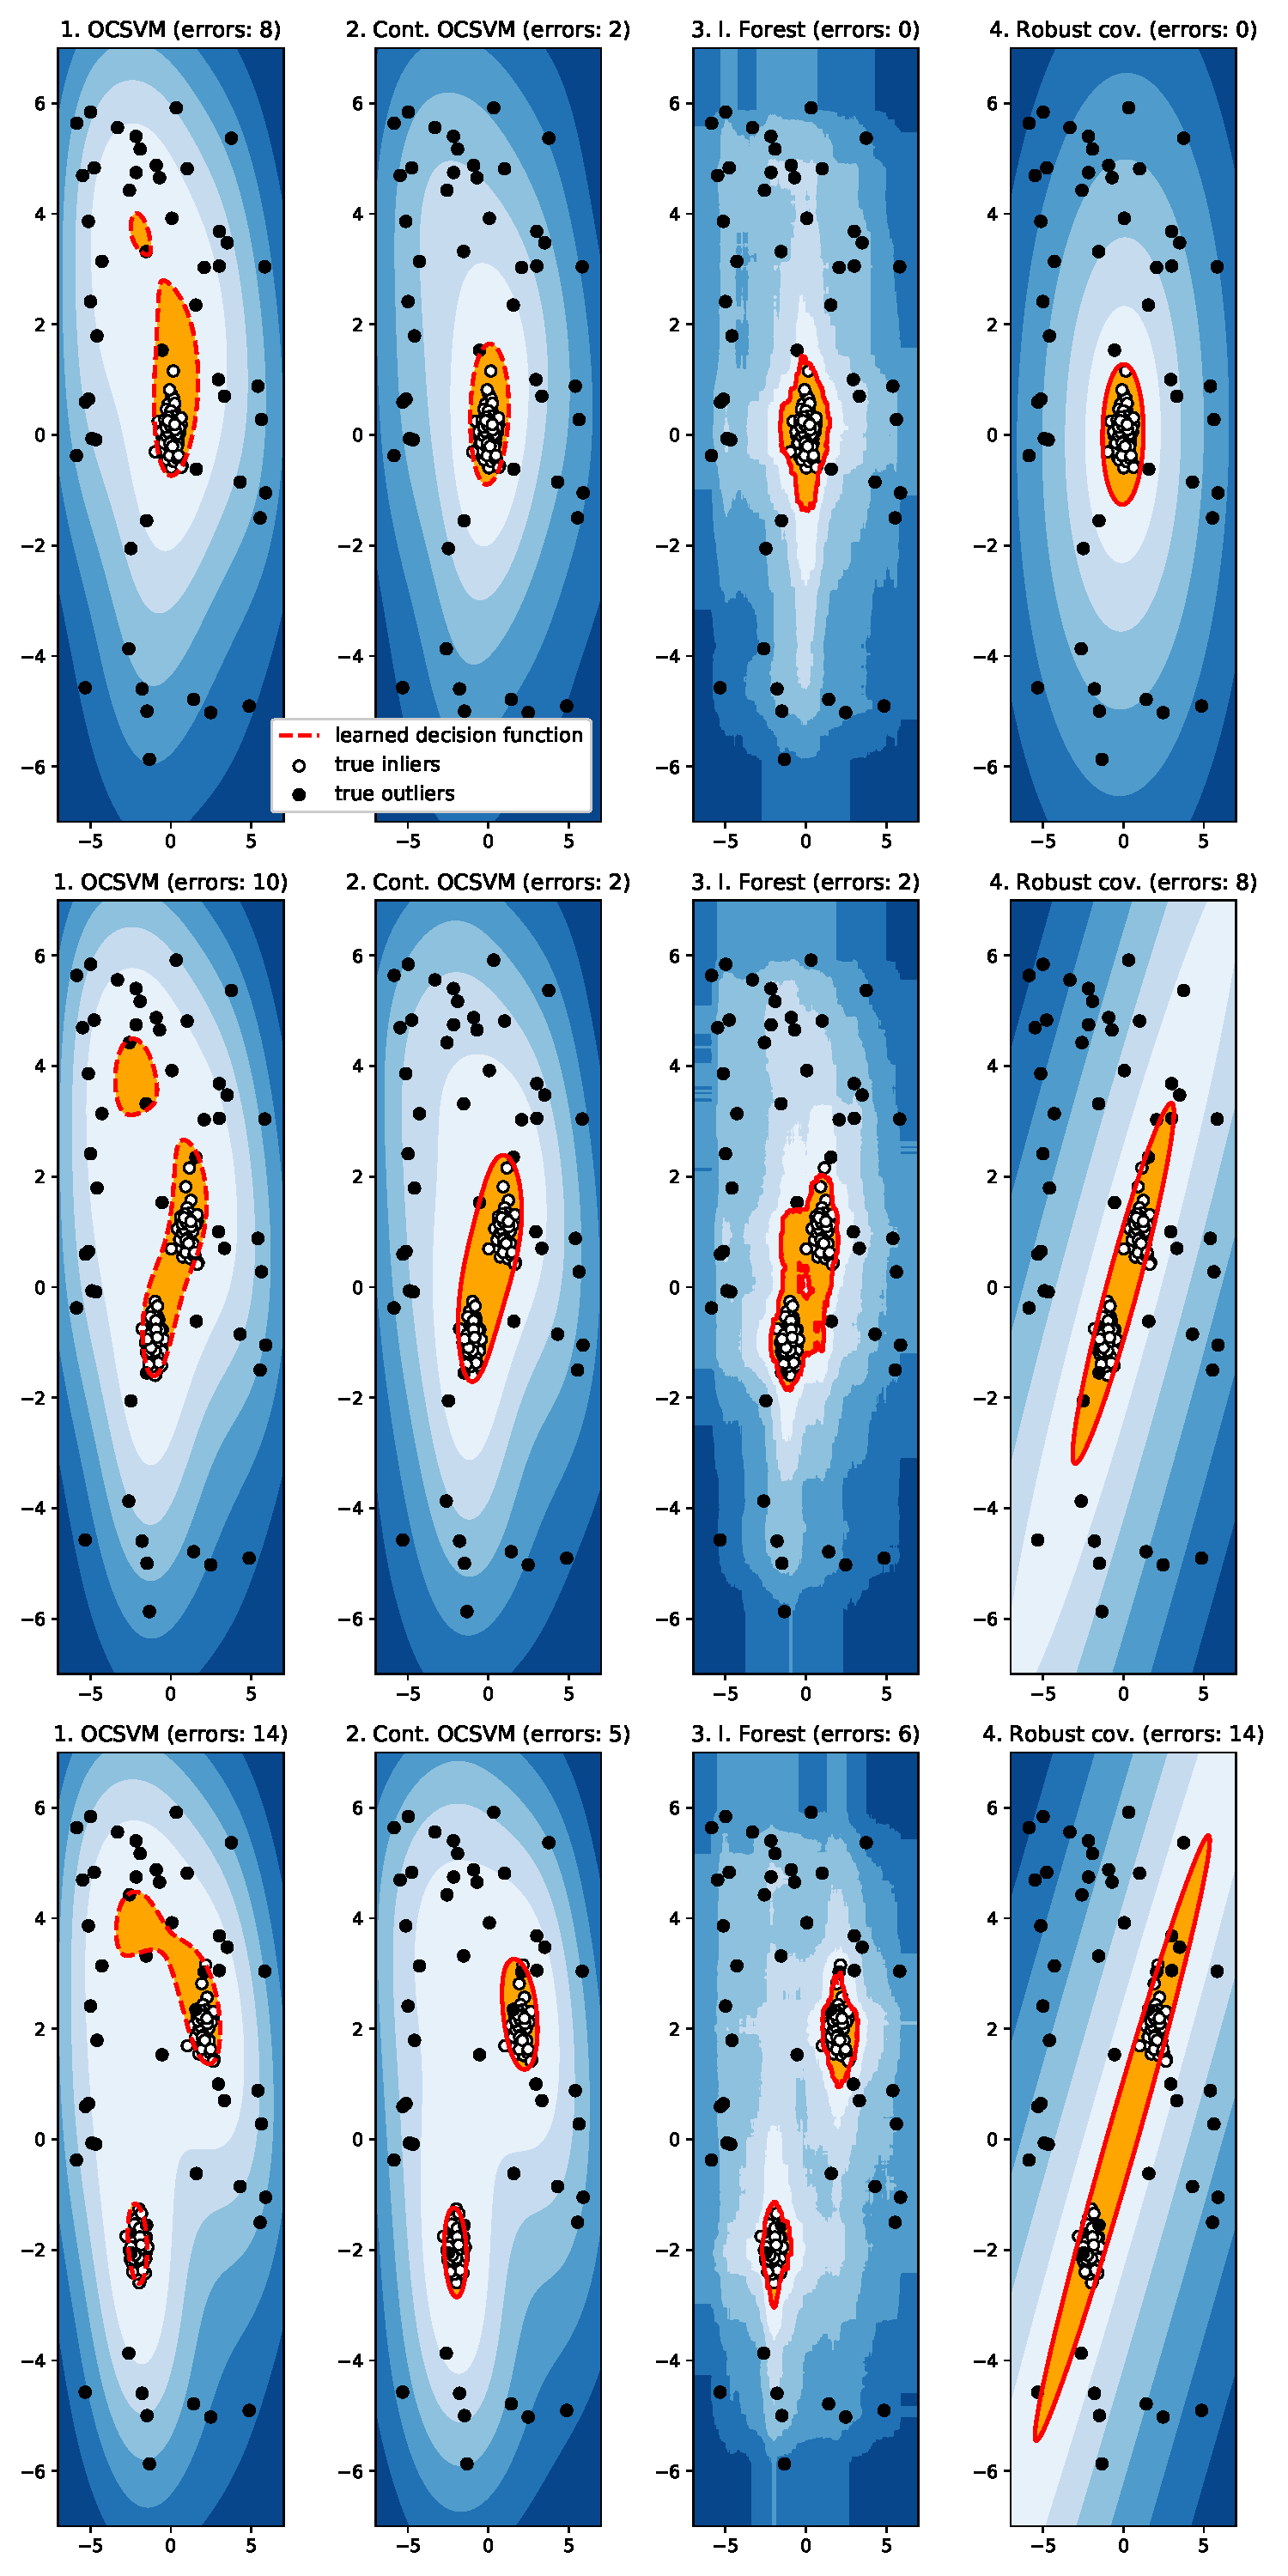
\includegraphics[width=\textwidth]{./gfx/ocsvm.eps}}
    %\caption[Continuous OCSVM for outlier detection]{Continuous OCSVM for
    %outlier detection. \label{fig:ocsvm_outlier}}
%\end{figure}
%\paragraph{}
%We propose a second experiment in a context of outlier detection. This time
%the train set is polluted with outliers. We replicate the example given in
%the documentations of Scikit-Learn at
%\url{http://scikit-learn.org/stable/auto_examples/covariance/plot_outlier_detection.html}
%We compare our method to three other well known outlier detection methods
%from the literature: Isolation Forest \citep{Liu2008}, \acs{OCSVM}
%\citep{Scholkopf2001} and a Robust Covariance estimator
%\citep{campbell1980robust, pedregosa2011scikit} on \cref{fig:ocsvm_outlier}.
%Our method achieve the state of the art on this simple example which is
%encouraging. However the computation time of our continuous \acs{OCSVM} is
%higher than the other methods. It took circa $0.25$ second for the \acs{OCSVM}.
%$10$ seconds for our method, $5$ seconds for isolation forest and $0.1$ second
%for the Robust covariance estimator. This can be due to the implementation since we used
%a (sub-optimal) hand-crafted full gradient descent. Notice that however our
%method is able to retrieve all the level sets after training, not only the one
%presented in \cref{fig:ocsvm_outlier}.  When one is interested in a specific
%level set or range of level set one could sample the $\nu_t$ from another
%distribution than the uniform distribution $\mathcal{U}[0, 1]$ to give more
%importance to the desire range of level sets.

%% %----------------------------------------------------------------------------
%% \section{The Nystr\"om method}
%% \label{sec:the_nystrom_method}

%% %----------------------------------------------------------------------------
%% \section{Sub-sampling the data}
%% \label{sec:sub_sampling_the_data}

%\section{Operalib}
%During this Thesis we started the development of a library named \say{Operalib}
%implementing various machine learning algorithms based on operator-valued
%kernels. Operator-valued kernels defines a framework allowing learning
%vector/function/structured output. The library currently features:
%\begin{itemize}
    %\item Quantile regression \citep{sangnier2016joint},
    %\item \acs{ONORMA} \citep{audiffren2013online},
    %\item semi-supervised Ridge regression \citep{Brouard2016_jmlr},
    %\item some elements of the \acs{ORFF} framework \citep{brault2016random}.
%\end{itemize}
%The algorithms work for a selection of popular operator-valued kernels such
%that the matrix-valued decomposable kernel, the curl-free kernel and the
%divergence-free kernel. The library is structured so that it is easy for the
%user to define its own operator-valued kernel and plug it to the existing
%optimisation algorithms, while keeping efficient computations thanks to the
%methodology presented in \cref{subsec:efficient_learning} (\acs{ie} by seeing
%operator-valued kernels as operators along with matrix-free solver rather than
%plain matrices). We designed the library in order to have a close compatibility
%with Scikit-learn. Code and documentation are publicly available at
%\url{https://github.com/operalib/operalib}. In a near future we plan to add the
%work of \citet{lim2015operator} for vector-autoregression with \acsp{OVK}. We
%hope to expand with more algorithms from various authors if the \acs{OVK}
%commutity and welcome any new contributor!

%\chapterend

\section{Learning function-valued functions}
In this section we show how to use \acs{OVK} in hand with the \acs{ORFF}
framework to learn function-valued functions. We focus on two application
cases: quantile regression and one-class classification. This section is rather
an informal (but detailed) discussion on ideas that we plan to improve for
future publications.

\subsection{Quantile regression}
\label{subsec:quantile_regression}
This introduction to quantile regression is adapted from the paper
of \citet{sangnier2016joint}. As we have seen in the introductory
\cref{ch:motivations}, a standard task in Machine Learning is to estimate the
conditional expectation $f(x)=\expectation_{\probability}[Y | X = x]$, where
$(X,Y)\sim\probability$ with some function belonging to a hypothesis space
$f\in\mathcal{F}$. Yet, many sensitive applications need more than the expected
valued of the relationship between random variables. To control the
\say{quality} of the predicted value from an input $x$, fields such as
economics, medicine, physics or social science require to have access to the
different quantile to model the distribution around the mean
$f(x)\in\mathbb{R}$ and strengthen their analysis.
\paragraph{}
Here we are interested in learning and predicting simultaneously \emph{all} the
quantiles on the compact $[0, 1]$, of the scalar-valued random variable $Y|X$.
We place ourselves in the setting of conditional quantile regression by
minimization of the pinball loss \citep{koenker1978regression}. For $\tau\in[0,
1]$ the pinball loss reads
\begin{dmath*}
    L_{\tau}(x, f, y) = \max(\tau \left(f(x) - y\right), (\tau - 1) \left(f(x)
    - y\right)).
\end{dmath*}
In a nutshell, this loss has been introduced by noticing that finding the
optimal location parameter $\mu = f(x)$ in the $\ell_1$ loss $L(x, f,
y)=\abs{f(x) - y}$ yields an estimator of the unconditional median
\citep{koenker1978regression}. Recently \citet{sangnier2016joint} proposed to
learn simultaneously many quantiles by minimizing the multi-quantile loss
function. Given a vector of quantiles $\boldsymbol{\tau} = (\tau_1, \dots
\tau_p)\in[0, 1]^p$
\begin{dmath*}
    L_{\boldsymbol{\tau}}(x, f, y) = \sum_{i=1}^p \max(\boldsymbol{\tau}_i
    \left(f(x)_i - y\right), (\boldsymbol{\tau}_i - 1)\left(f(x)_i - y\right)).
\end{dmath*}
We see that now it is necessary for $f(x)\in\mathbb{R}^p$ to be vector-valued.
In this work we push further the idea by considering that $f(x)$ is a function
of an arbitrary quantile $\tau\in[0, 1]$. Thus we view $f$ as a vector-valued
function $f:\mathbb{R} \to ([0, 1] \to \mathbb{R})$. For the sake of simplicity
we note $f(x)=f_x$ and introduce the generalized pinball loss
\begin{dmath}
    \label{eq:loss_pinball}
    L(x, f, y) = \int_{[0, 1]} \max(\tau \left(f_x(\tau) - y\right), (\tau -
    1)\left(f_x(\tau) - y)\right) d\tau.
\end{dmath}

\subsection{Functional output data}
Pioneer work on learning function-valued function has been done by
\citet{kadri2015operator}. Inspired by them we develop an \acs{ORFF}
methodology to learn functional data where the outputs are functions that we
suppose living in a \acs{RKHS}.
\paragraph{}
Namely, we suppose that the image of a funtion $f$, has values $f(x) \in
\mathcal{H}_{k_{\mathcal{T}}}$ in a \acs{RKHS}, where
$k_{\mathcal{T}}:\mathcal{T}^2\to\mathbb{R}$ is a scalar-valued kernel and
$\mathcal{H}_{k_{\mathcal{T}}}$ is the corresponding \acs{RKHS}. From this
hypothesis we see that
\begin{dmath*}
    f_x(\tau) = \inner{f(x), k_{\mathcal{T}}(\cdot,
    \tau)}_{\mathcal{H}_{k_{\mathcal{T}}}}
\end{dmath*}
If we add the second hypothesis that $f\in\mathcal{H}_K$, where $\mathcal{H}_K$
is a \emph{\acl{vv-RKHS}} for some \acl{OVK} $K$, \Citet{Carmeli2010} showed in
example $6$ page $17$-$18$ that in this case the operator $K$ is given by
\begin{dmath}
    \label{eq:functional_kernel}
    K =
    \begin{cases}
        \mathcal{X} \times \mathcal{X} & \to
        \mathcal{L}(\mathcal{H}_{k_{\mathcal{T}}}) \\
        x, z & \mapsto k_{\mathcal{X}}(x, z) I_{\mathcal{H}_{k_{\mathcal{T}}}},
    \end{cases}
\end{dmath}
where $k:\mathcal{X}\times\mathcal{X} \to \mathbb{R}$ is another scalar-valued
kernel. Moreover \citet{Carmeli2010} showed in example $7$ page $18$-$19$ that
the \acs{vv-RKHS} induced by $K$ is the same \acs{RKHS} than the one induced by
the kernel $K'$ defined as follow for some measure $\mu$ with support
$\mathcal{T}$.
\begin{dmath*}
    K' =
    \begin{cases}
        \mathcal{X} \times \mathcal{X} & \to
        \mathcal{L}\left(L^2(\mathcal{T}, \mu)\right) \\
        x, z & \mapsto \left(g \mapsto k_{\mathcal{X}}(x, z)
        \int_{\mathcal{T}}k_{\mathcal{T}}(\cdot, \tau)g(\tau)d\mu(\tau)\right).
    \end{cases}
\end{dmath*}
This is exactly the decomposable kernel introduced in
\cref{def:hilbert_schmidt_integral_kernel} in \cref{ch:motivations}. Because
the \acsp{RKHS} induced by $K$ and $K'$ is the same, we can either view its
elements as functions from $\mathcal{X}$ into $\mathcal{H}_{k_{\mathcal{T}}}$
(through $\mathcal{H}_K$) or as functions from $\mathcal{X}$ into
$L^2(\mathcal{T}, \mu)$ (through $\mathcal{H}_{K'}$).

\subsection{ORFF for functional output data}
Because $\mathcal{Y}=\mathcal{H}_{k_{\mathcal{T}}}$ is a proper (infinite
dimensional) Hilbert space, we can apply the \acs{ORFF} methodology. Let
$k_{\mathcal{X}}$ be a scalar Mercer kernel and $\mathcal{X}=\mathbb{R}$. Then
by \cref{cr:ORFF-map-kernel} applied to the decomposable kernel (see
\cref{subsec:examples_ORFF}) we have the following approximate feature map for
$K$ defined in \cref{eq:functional_kernel}:
\begin{dmath*}
    \tildePhi{\omega}(x)y = \frac{1}{\sqrt{D}}\Vect_{j=1}^D
    \begin{pmatrix}
        \cos(x \omega_j) B^\adjoint y \\
        \sin(x \omega_j) B^\adjoint y
    \end{pmatrix} \condition{$\omega_j \sim \FT{k_{\mathcal{X}}}$
    \ac{iid}}
\end{dmath*}
where $BB^\adjoint = I_{\mathcal{H}_{k_{\mathcal{T}}}}$ and
$y\in\mathcal{H}_{k_{\mathcal{T}}}$. At this point we could choose
$B=I_{\mathcal{H}_{k_{\mathcal{T}}}}$. However this is not really useful since
it would make the redescription space $\widetilde{\mathcal{H}}=\Vect_{j=1}^D
\mathcal{H}_{k_{\mathcal{T}}}$, which is a direct sum of infinite dimensional
\acs{RKHS}. Yet since $\mathcal{H}_{k_{\mathcal{T}}}$ is a \acs{RKHS},
according to \cref{pr:feature_operator} it is possible to define a feature
operator $W:\mathcal{H}\to\mathcal{H}_{k_{\mathcal{T}}}$ such that
$(Wg)(\tau)=\Phi_\tau^\adjoint g$.
\maxdeadcycles=10000
\afterpage{%
\begin{landscape}
    \begin{figure}[htp]
        \centering
        \resizebox{.8\textheight}{!}{%
        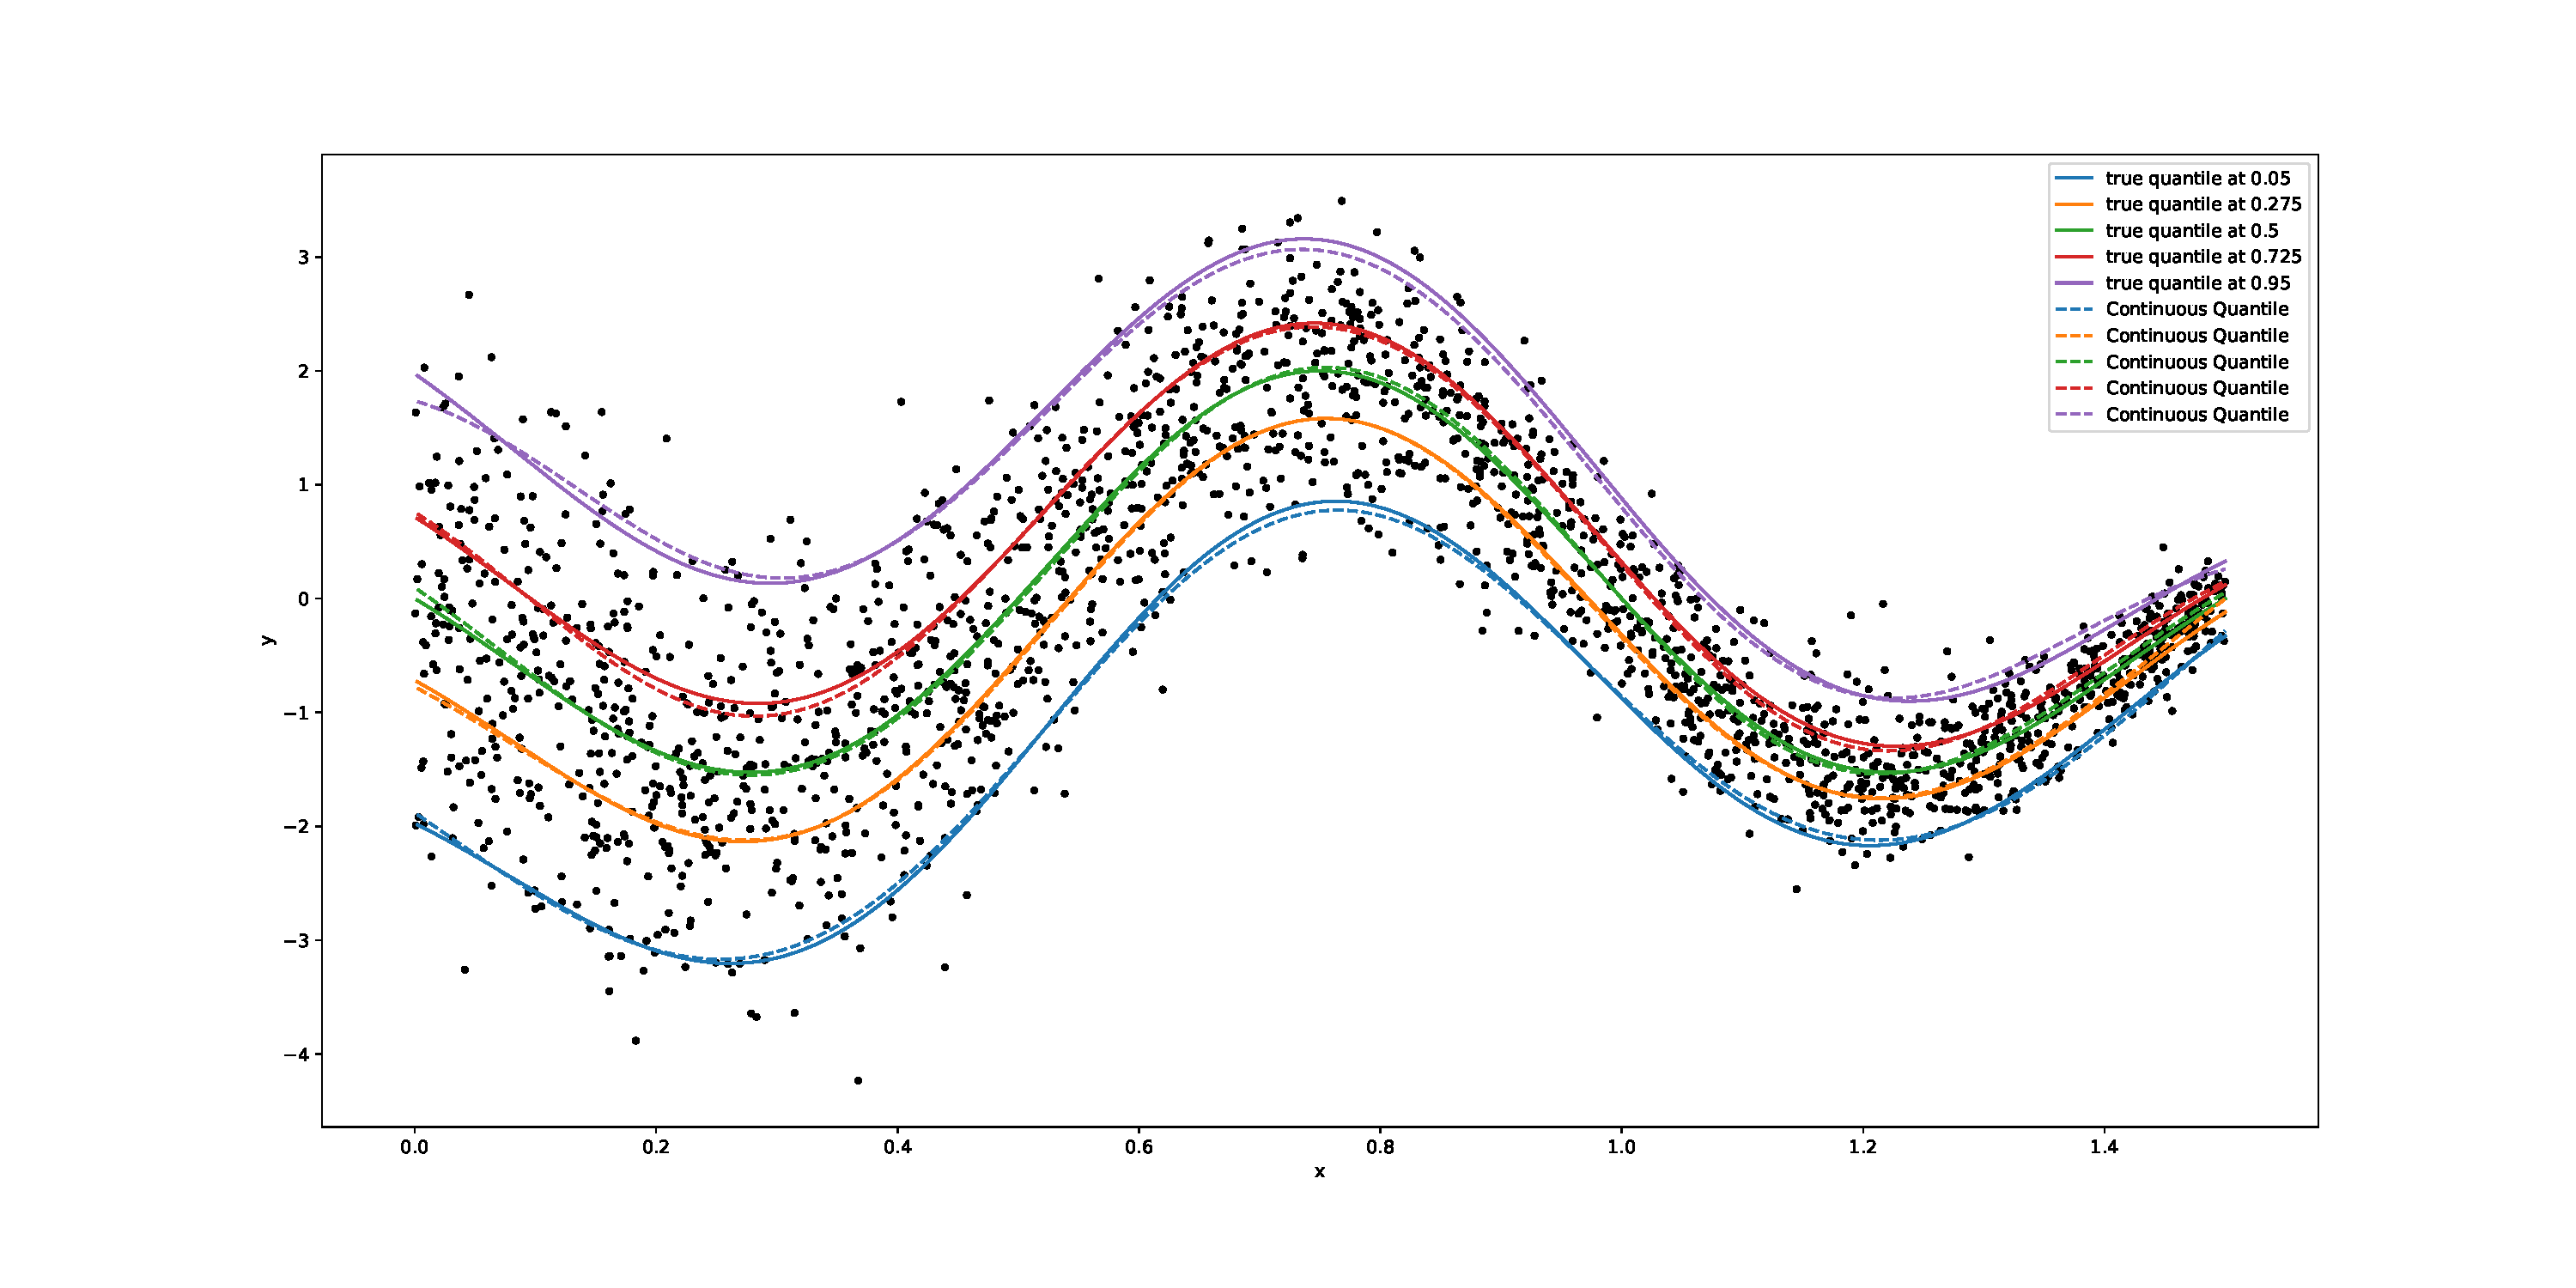
\includegraphics{./gfx/quantile_orff.pdf}}
        \caption{Learning a continuous quantile function with ORFF
        regression. \label{fig:quantile_orff}}
    \end{figure}
    \clearpage
    \begin{figure}[htp]
        \centering\resizebox{.8\textheight}{!}{%
        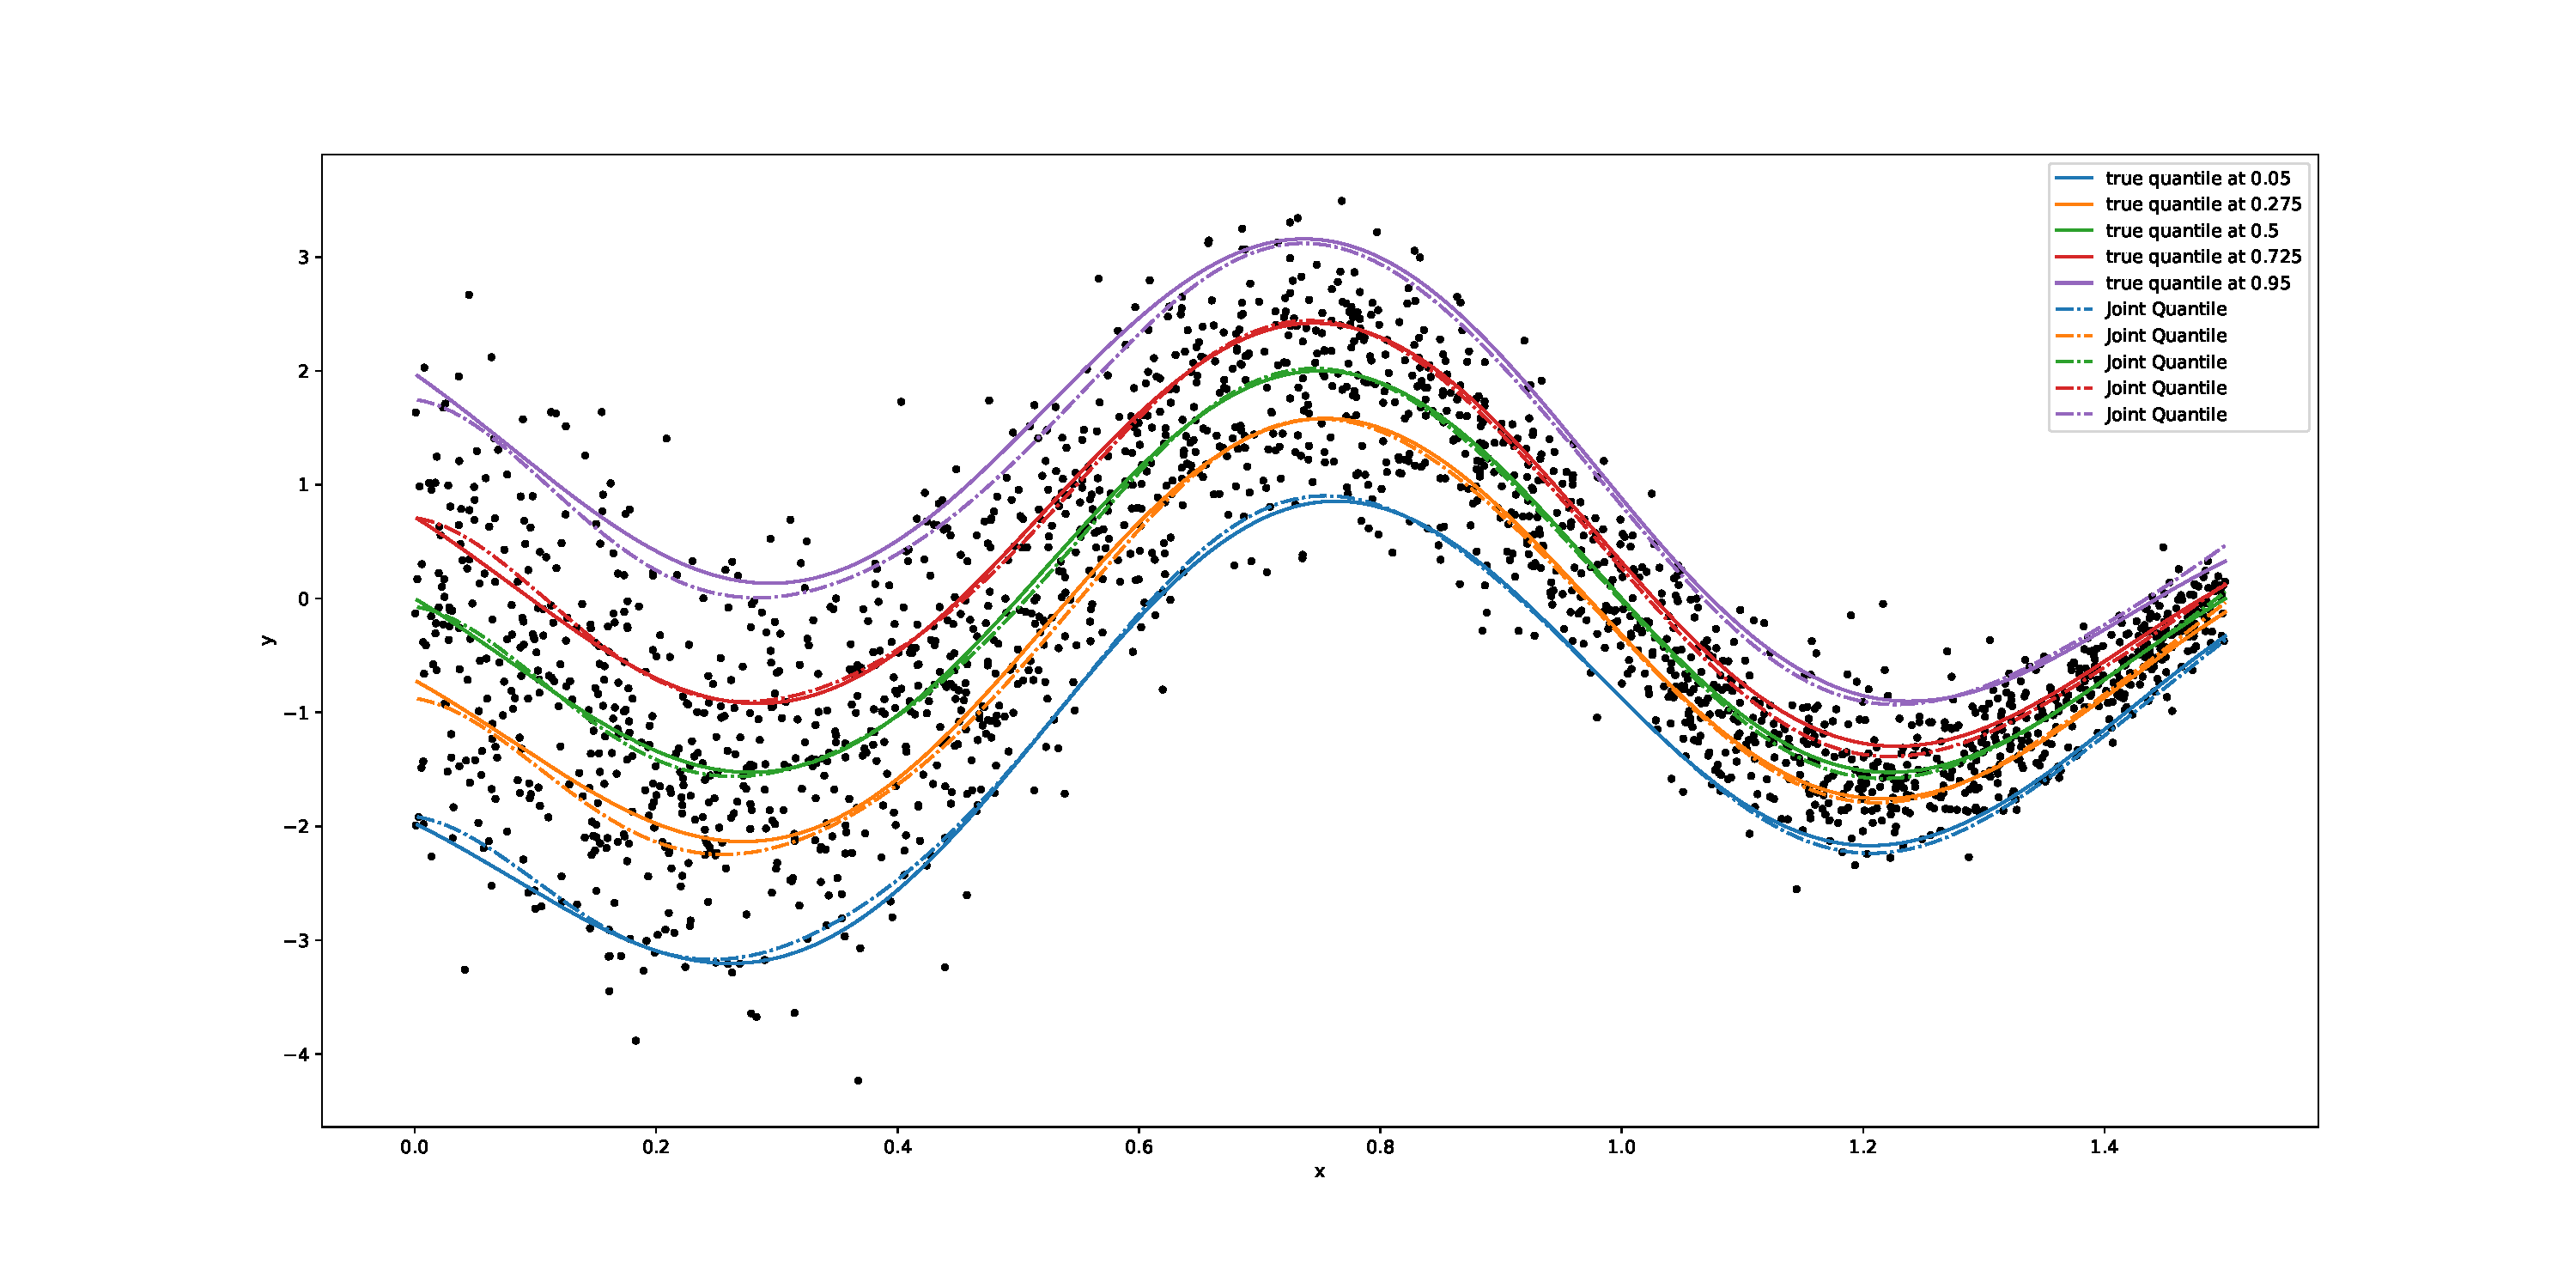
\includegraphics{./gfx/quantile_joint.pdf}}
        \caption{Learning many quantile with joint OVK regression.
        \label{fig:quantile_joint}}
    \end{figure}
\end{landscape}}
Moreover $W^\adjoint W$ is the identity on
$\Ima \Phi_{\tau}$ which is here $\mathcal{H}_{k_{\mathcal{T}}}$. (see the
proof of \cref{pr:feature_operator} and \citet{Carmeli2010}). Thus we can
choose $\Phi_\tau=\Phi(\tau)$ to be the functional Fourier feature map
associated to $k_{\mathcal{T}}$ defined in \cref{pr:fourier_feature_map}.  Then
we have $BB^\adjoint = I_{\mathcal{H}_{k_{\mathcal{T}}}} = W W^\adjoint$.  Thus
we can choose $B = W = \Phi(\cdot)^\adjoint$ and the approximate
feature map reads
\begin{dmath*}
    \tildePhi{\omega}(x)\in \mathcal{L}\left(\mathcal{H}_{k_{\mathcal{T}}};
    \Vect_{j=1}^D L^2\left(\dual{\mathcal{T}},
    \probability_{\dual{\Haar},\rho}\right)\right)
\end{dmath*}
and
\begin{dmath*}
    (\tildePhi{\omega}(x)g)(\tau) = \frac{1}{\sqrt{D}}\Vect_{j=1}^D
    \begin{pmatrix}
        \cos(x \omega_j) W^\adjoint g \\
        \sin(x \omega_j) W^\adjoint g
    \end{pmatrix} \condition{$\omega_j \sim \FT{k_{\mathcal{X}}}$
    \ac{iid}}
\end{dmath*}
%Then as proposed in \cref{ch:operator-valued_random_fourier_features} we can
%Monte-Carlo sample the functional feature map $\Phi(\tau)$ and obtain the
%\acs{ORFF} map
%\begin{dmath*}
    %\left(\widetilde{\tildePhi{\omega}}(x)g\right)(\tau) =
    %\frac{1}{\sqrt{DD'}}\Vect_{j=1}^D
    %\begin{pmatrix}
        %\cos(x \omega_j) \sum_{k=1}^{D'}
        %\left(\cos(\tau \omega_k') + \sin(\tau \omega_k')\right)g(\omega_k') \\
        %\sin(x \omega_j) \sum_{k=1}^{D'}
        %\left(\cos(\tau \omega_k') + \sin(\tau \omega_k')\right)g(\omega_k')
    %\end{pmatrix} \condition{$\omega_j \sim \FT{k_{\mathcal{X}}}$
    %\acs{iid} and $\omega_k'\sim \FT{k_{\mathcal{T}}}$ \acs{iid}.}
%\end{dmath*}
%where $g\in L^2\left(\dual{\mathcal{T}}, \probability_{\dual{\Haar},
%\rho}\right)$ and $\tau\in\mathbb{R}$. If we note
%\begin{dmath*}
    %G =
    %\begin{pmatrix}
        %g(\omega_1') & \dots & g(\omega_{D'}')
    %\end{pmatrix}^\adjoint \hiderel{\in} \mathbb{R}^{D'}
%\end{dmath*}
%we can define
%\begin{dmath*}
    %\left(\widetilde{\tildePhi{\omega}}(x)G\right)(\tau) =
    %\frac{1}{\sqrt{DD'}}\Vect_{j=1}^D
    %\begin{pmatrix}
        %\cos(x \omega_j) \sum_{k=1}^{D'}
        %\left(\cos(\tau \omega_k') + \sin(\tau \omega_k')\right)G_k \\
        %\sin(x \omega_j) \sum_{k=1}^{D'}
        %\left(\cos(\tau \omega_k') + \sin(\tau \omega_k')\right)G_k
    %\end{pmatrix} \condition{$\omega_j \sim \FT{k_{\mathcal{X}}}$
    %\acs{iid} and $\omega_k'\sim \FT{k_{\mathcal{T}}}$ \acs{iid}.}
%\end{dmath*}
Then it is easy to verify that the adjoint operator is given by
\begin{dmath*}
    \left(\widetilde{\tildePhi{\omega}}(x)^\adjoint \theta\right)(\tau) =
    \frac{1}{\sqrt{DD'}} \sum_{j=1}^D \left(\cos(x\omega_j) +
    \sin(x\omega_j)\right) \left(\Vect_{k=1}^{D'}
    \begin{pmatrix}
        \cos(\tau \omega_k') \\
        \sin(\tau \omega_k')
    \end{pmatrix}\right)^\adjoint \theta_j
    = \frac{1}{\sqrt{DD'}} \sum_{j=1}^D \left(\cos(x\omega_j) +
    \sin(x\omega_j)\right) \theta_{jk} \left( \cos(\tau \omega_k') + \sin(\tau
    \omega_k')\right)
    \condition{$\omega_j \sim \FT{k_{\mathcal{X}}}$
    \acs{iid} and $\omega_k'\sim \FT{k_{\mathcal{T}}}$ \acs{iid}.}
\end{dmath*}
where $\theta_k\in\mathbb{R}^{D'}$, for all $k \in \mathbb{N}^*_D$ and
$\theta_{jk}\in\mathbb{R}$ for all $j \in \mathbb{N}^*_D$ and all $k \in
\mathbb{N}^*_{D'}$. The above equations can be rewritten in matrix form which
results in the following conjecture.
\begin{conjecture}
    \label{cj:functional_orff}
    If $\tildephi{\omega}_{\mathcal{X}}$ is an \acs{RFF} for
    $\widetilde{k}_{\mathcal{X}}$ such that
    $\tildephi{\omega}(x)\in\mathbb{R}^D$ and $\tildephi{\omega}_{\mathcal{T}}$
    is an \acs{RFF} for $\widetilde{k}_{\mathcal{T}}$, such that
    $\tildephi{\omega}(\tau)\in\mathbb{R}^{D'}$ then an \acs{ORFF} map for
    \begin{dmath*}
        K(x, z) = k_{\mathcal{X}}(x, z)
        I_{\mathcal{H}_{\tilde{k}_{\mathcal{T}}}}
    \end{dmath*}
    is given for all $x\in\mathbb{R}$, all $\tau\in\mathbb{R}$ and all
    $\Theta\in\mathcal{M}_{D,D'}(\mathbb{R})$ by
    \begin{dmath*}
        \left(\tildePhi{\omega}_K(x)^\adjoint \Theta \right)(\tau) =
        \tildephi{\omega}_{\mathcal{X}}(x)^\adjoint \Theta
        \tildephi{\omega}_{\mathcal{T}}(\tau)
    \end{dmath*}
    and
    \begin{dmath*}
        \left(\tildePhi{\omega}_K(x) G\right)(\tau) =
        \tildephi{\omega}_{\mathcal{X}}(x)
        \tildephi{\omega}_{\mathcal{T}}(\tau)^\adjoint G,
    \end{dmath*}
    where $g\in\mathbb{R}^{D'}$.
    %but more intestingly, given $y\in\mathbb{R}$,
    %\begin{dmath*}
        %\tildePhi{\omega}_K(x, \tau)^\adjoint y =
        %y \tildephi{\omega}_{\mathcal{X}}(x)
        %\tildephi{\omega}_{\mathcal{T}}(\tau)^\adjoint.
    %\end{dmath*}
\end{conjecture}
Moreover if one defines $\tildePhi{\omega}_K(x,
\tau) = \left(\tildePhi{\omega}_K(x)^\adjoint \Theta \right)(\tau)$ one
have of course
\begin{dmath*}
    \tildePhi{\omega}_K(x, \tau)^\adjoint \Theta =
    \tildephi{\omega}_{\mathcal{X}}(x)^\adjoint \Theta
    \tildephi{\omega}_{\mathcal{T}}(\tau)
\end{dmath*}
\subsection{Many quantile regression}
From the loss defined in \cref{eq:loss_pinball} we defined the regularized risk
using the \say{continuous} pinball loss for the quantile regression problem.
For all $f\in\mathcal{H}_K$,
\begin{dmath*}
    \mathfrak{R}_{\lambda}(f, \seq{s}) =
    \frac{1}{N}\sum_{i=1}^N\int_{[0,1]}\left(
    \begin{cases}
        \tau\left(f_{x_i}(\tau) - y_i\right) & \text{if } f_{x_i}(\tau) \ge y_i
        \\
        (1 - \tau)\left(y_i - f_{x_i}(\tau)\right) & \text{otherwise}
    \end{cases} \right)+ \lambda
    \norm{f}_K^2.
\end{dmath*}
The issue with the above risk is that the different quantile for a given point
$x\in\mathbb{R}$ may cross (see \citet{sangnier2016joint}). To avoid this to
happen we need to force the function $f_x(\tau)$ to be \emph{increasing} in
$\tau$ for any $x\in\mathbb{R}$.  Because a decreasing function has a negative
derivative we can add a penalty term to the risk to avoid $f_x(\tau)$ to be
decreasing in $\tau$.
\begin{dmath*}
    \Omega_{cross}(f_{x_i}) = - \min\left(\frac{\partial
    f_{x_i}}{\partial\tau}(\tau),
    0\right)
\end{dmath*}
Thus the regularized risk with the no crossing constraint is
\begin{dmath*}
    \mathfrak{R}_{\lambda_1, \lambda_2}(f, \seq{s}) =
    \frac{1}{N}\sum_{i=1}^N\int_{[0,1]}\left(
    \begin{cases}
        \tau \left(f_{x_i}(\tau) - y_i\right) & \text{if } f_{x_i}(\tau) \ge
        y_i \\
        (1 - \tau)\left(y_i - f_{x_i}(\tau)\right) & \text{otherwise}
    \end{cases} -
    \lambda_1 \min\left(\frac{\partial f_{x_i}}{\partial\tau}(\tau), 0\right)
    \right)+ \lambda_2 \norm{f}_K^2.
\end{dmath*}
Eventually we replace the integral by a Monte-Carlo sampling with the uniform
law $\mathcal{U}([0, 1])$ and plug in the approximate function of $f$ using the
\acs{ORFF} map proposed in \cref{cj:functional_orff}. The final regularized
risk to be minimized reads
\begin{dmath*}
    \mathfrak{R}_{\lambda_1, \lambda_2}(\Theta, \seq{s}) =
    \frac{1}{NT}\sum_{i=1}^N\sum_{t=1}^T\left(
    \begin{cases} \tau_t
        \left(\widetilde{f}_{x_i}(\tau_t) - y_i\right) & \text{if }
        \widetilde{f}_{x_i}(\tau_t) \ge y_i \\
        (1 - \tau_t)\left(y_i - f_{x_i}(\tau_t)\right) & \text{otherwise}
    \end{cases} - \lambda_1
    \min\left(\frac{\partial \widetilde{f}_{x_i}}{\partial\tau}(\tau_t),
    0\right) \right)+ \lambda_2 \norm{\Theta}_{fro}^2.
\end{dmath*}
where $\widetilde{f}_{x}(\tau)=\tildephi{\omega}_{\mathcal{X}}(x)^\adjoint
\Theta \tildephi{\omega}_{\mathcal{T}}(\tau)$, $\tau_t \sim \mathcal{U}([0,
1])$ and
\begin{dmath*}
    \frac{\partial \widetilde{f}_{x}}{\partial\tau}(\tau)
    = \tildephi{\omega}_{\mathcal{X}}(x)^\adjoint \Theta \frac{\partial
    \tildephi{\omega}_{\mathcal{T}}}{\partial \tau}(\tau)
    = \tildephi{\omega}_{\mathcal{X}}(x)^\adjoint \Theta \Vect_{k=1}^{D'}
    \begin{pmatrix}
        -\omega_k' \sin(\omega_k' \tau) \\
         \omega_k' \cos(\omega_k' \tau)
    \end{pmatrix} \condition{$\omega_k' \sim \FT{k_{\mathcal{T}}}$ \acs{iid}.}
\end{dmath*}
\subsubsection{Some results}
We minimized the quantity $\mathfrak{R}_{\lambda_1, \lambda_2}(\Theta,
\seq{s})$ on a toy dataset: a sine wave with some heteroscedastic noise. First
we compared our methodology to the joint quantile regression proposed in
\citet{sangnier2016joint}. We generate $N=2500$ for the train set and $N'=1000$
points for the test set and use a Gaussian kernel for both $k_{\mathcal{X}}$
and $k_{\mathcal{T}}$. We choosed $\sigma_{\mathcal{X}} = 0.25$ and
$\sigma_{\mathcal{T}}$ has been set to be the median of the pairwise distance
of the $\tau_t$'s drawn randomly from $\mathcal{U}([0, 1])$. Notice that
$\mathfrak{R}_{\lambda_1, \lambda_2}(\Theta, \seq{s})$ is convex in $\Theta$.
To avoid computing complex gradients and by lack of time, we used Tensorflow
\citep{abadi2016tensorflow} to perform a gradient descent (with RMSProp
\citep{tieleman2012lecture}) with automatic symbolic differentiation.
\Cref{fig:quantile_orff} show the result for the quantile at $0.05$, $0.275$,
$0.5$, $0.775$ and $0.95$ using the \acs{ORFF} methodology.
\afterpage{%
\begin{landscape}
    \begin{figure}[htp]
        \centering
        \resizebox{.8\textheight}{!}{%
        \includegraphics{./gfx/quantile_continuous.pgf}}
        \caption{Learning a continuous quantile function with ORFF
        regression. \label{fig:quantile_continuous}}
    \end{figure}
\end{landscape}}
\Cref{fig:quantile_joint} shows the joint quantile regression of
\citet{sangnier2016joint} on the same dataset. Not only our method matched the
the performances of \citet{sangnier2016joint}\footnote{We reported an error
computed with the pinball loss on the test set of $0.818$ for our method and
$0.817$ for joint regression (note that we don't report here an average on many
experiments to avoid randomness introduced by the random features, but the
results seems robust in practice.)} but we cutted down the computation time
from circa $1330$ seconds to circa $30$ seconds (training and testing).
Moreover on contrary to \citet{sangnier2016joint} we have access to all the
quantile of the model (see \cref{fig:quantile_continuous}).

\subsection{One-class SVM revisited}
We also propose an extension of the celebrated \acf{OCSVM} such that it is
possible to learn jointly all the level sets.  One-class classification, also
known as unary classification, tries to identify objects of a specific class
amongst all objects, by learning from a training set containing only the
objects of that class.  In this framework, we assume that we only observe
examples of one class (referred to as the inlier class).  The second class is
called outlier class.  We turn our attention to the \acs{OCSVM}
of \citet{Scholkopf2001} which extends the \ac{SVM} methodology
\citep{Cortes1995,Shawe2004} to handle training using only inliers.
\paragraph{}
We recall that given an hyperparameter $\nu\in [0,1]$ that controls the
proportion of inlier, given as scalar kernel $k$, the \acs{OCSVM} problem reads
\begin{dmath*}
    \argmin_{f\in\mathcal{H}_k, \tau \in \mathbb{R}} \frac{\nu}{2}
    \norm{f}_{\mathcal{H}_k}^2 - \nu \tau + \frac{1}{N} \sum_{i=1}^N \max(\tau
    - f(x_i), 0)
\end{dmath*}
The decision function is then
\begin{dmath*}
    h(x, \tau) = \mathds{1}_{[\tau, \infty)}\left( f(x) \right).
\end{dmath*}
As in \cref{subsec:quantile_regression} we can rewrite the optimization problem
as an integral over all the value of $\nu$ and suppose that $f$ is
function-valued (a function of $\nu$). Moreover $\tau$ must also change its
value according to $\nu$. Thus given a kernel $k_{\mathcal{X}}$ on the inputs
$x\in\mathbb{R}^d$ with its approximate feature map
$\tildephi{\omega}_{\mathcal{X}}$ and a kernel $k_{\mathcal{T}}$ on the level
sets with its approximate feature map $\tildephi{\omega}_{\mathcal{T}}$, we
define the continuous one-class SVM problem as
\begin{dmath*}
    \argmin_{f
    \in\mathcal{H}_K,\tau\in\mathcal{H}_{k_{\tau}}}\frac{1}{N}
    \sum_{i=1}^N\int_{[0,1]}\max\left(0, \tau(\nu) - f_{x_i}(\nu)\right)d\nu +
    \frac{1}{2}\int_{[0,1]}\nu
    \norm{f_{\cdot}(\nu)}_{\mathcal{H}_{k_{\mathcal{X}}}}^2d\nu -
    \int_{[0,1]}\nu\tau(\nu)d\nu.
\end{dmath*}
Again we can compute the integral by Monte-Carlo sampling and replace $f$ and
$\tau$ by their respective approximation. Notice that the \acs{RKHS} of $\tau$
should match the \acs{RKHS} of the output space of $f_K$. Hence
\begin{dmath*}
    \argmin_{\Theta
    \in\mathcal{M}_{D, D'}(\mathbb{R}),\tau\in\mathbb{R}^D}\frac{1}{NT}
    \sum_{i=1}^N\sum_{t=1}^T\max\left(0, \widetilde{\tau}(\nu_t) -
    \widetilde{f}_{x_i}(\nu_t)\right) + \frac{1}{2T}\sum_{t=1}^T\nu_t
    \norm{\widetilde{f}_{\cdot}(\nu_t)}_{2}^2 -
    \frac{1}{T}\sum_{t=1}^T\nu_t\widetilde{\tau}(\nu_t),
\end{dmath*}
where $\nu_t \sim \mathcal{U}([0, 1])$ \acs{iid}, $\widetilde{\tau}(\nu) =
\tildephi{\omega}_{\mathcal{T}}(\nu)$ and $\widetilde{f}_x(\nu) =
\tildephi{\omega}(x)^\adjoint \Theta \tildephi{\omega}_{\mathcal{T}}(\nu)$. We
also deduce that $\widetilde{f}_{\cdot}(\nu) = \Theta
\tildephi{\omega}_{\mathcal{T}}(\nu)$. Here the natural decision function is
\begin{dmath}
    \label{eq:continuous_decision}
    h(x, \nu) = \mathds{1}_{\left[\widetilde{\tau}(\nu),\infty\right)}
    \left(\widetilde{f}_x(\nu)\right).
\end{dmath}
\begin{figure}
    {\centering
    \resizebox{2\textwidth}{!}{%% Creator: Matplotlib, PGF backend
%%
%% To include the figure in your LaTeX document, write
%%   \input{<filename>.pgf}
%%
%% Make sure the required packages are loaded in your preamble
%%   \usepackage{pgf}
%%
%% Figures using additional raster images can only be included by \input if
%% they are in the same directory as the main LaTeX file. For loading figures
%% from other directories you can use the `import` package
%%   \usepackage{import}
%% and then include the figures with
%%   \import{<path to file>}{<filename>.pgf}
%%
%% Matplotlib used the following preamble
%%   \usepackage{fontspec}
%%   \setmainfont{Times New Roman}
%%   \setsansfont{Lucida Grande}
%%   \setmonofont{Andale Mono}
%%
\begingroup%
\makeatletter%
\begin{pgfpicture}%
\pgfpathrectangle{\pgfpointorigin}{\pgfqpoint{16.000000in}{5.000000in}}%
\pgfusepath{use as bounding box, clip}%
\begin{pgfscope}%
\pgfsetbuttcap%
\pgfsetmiterjoin%
\definecolor{currentfill}{rgb}{1.000000,1.000000,1.000000}%
\pgfsetfillcolor{currentfill}%
\pgfsetlinewidth{0.000000pt}%
\definecolor{currentstroke}{rgb}{1.000000,1.000000,1.000000}%
\pgfsetstrokecolor{currentstroke}%
\pgfsetdash{}{0pt}%
\pgfpathmoveto{\pgfqpoint{0.000000in}{0.000000in}}%
\pgfpathlineto{\pgfqpoint{16.000000in}{0.000000in}}%
\pgfpathlineto{\pgfqpoint{16.000000in}{5.000000in}}%
\pgfpathlineto{\pgfqpoint{0.000000in}{5.000000in}}%
\pgfpathclose%
\pgfusepath{fill}%
\end{pgfscope}%
\begin{pgfscope}%
\pgfsetbuttcap%
\pgfsetmiterjoin%
\definecolor{currentfill}{rgb}{1.000000,1.000000,1.000000}%
\pgfsetfillcolor{currentfill}%
\pgfsetlinewidth{0.000000pt}%
\definecolor{currentstroke}{rgb}{0.000000,0.000000,0.000000}%
\pgfsetstrokecolor{currentstroke}%
\pgfsetstrokeopacity{0.000000}%
\pgfsetdash{}{0pt}%
\pgfpathmoveto{\pgfqpoint{0.663889in}{0.580556in}}%
\pgfpathlineto{\pgfqpoint{8.157639in}{0.580556in}}%
\pgfpathlineto{\pgfqpoint{8.157639in}{4.801389in}}%
\pgfpathlineto{\pgfqpoint{0.663889in}{4.801389in}}%
\pgfpathclose%
\pgfusepath{fill}%
\end{pgfscope}%
\begin{pgfscope}%
\pgfsetbuttcap%
\pgfsetroundjoin%
\definecolor{currentfill}{rgb}{0.000000,0.000000,0.000000}%
\pgfsetfillcolor{currentfill}%
\pgfsetlinewidth{0.803000pt}%
\definecolor{currentstroke}{rgb}{0.000000,0.000000,0.000000}%
\pgfsetstrokecolor{currentstroke}%
\pgfsetdash{}{0pt}%
\pgfsys@defobject{currentmarker}{\pgfqpoint{0.000000in}{-0.048611in}}{\pgfqpoint{0.000000in}{0.000000in}}{%
\pgfpathmoveto{\pgfqpoint{0.000000in}{0.000000in}}%
\pgfpathlineto{\pgfqpoint{0.000000in}{-0.048611in}}%
\pgfusepath{stroke,fill}%
}%
\begin{pgfscope}%
\pgfsys@transformshift{1.004514in}{0.580556in}%
\pgfsys@useobject{currentmarker}{}%
\end{pgfscope}%
\end{pgfscope}%
\begin{pgfscope}%
\pgftext[x=1.004514in,y=0.483333in,,top]{\sffamily\fontsize{10.000000}{12.000000}\selectfont 0.0}%
\end{pgfscope}%
\begin{pgfscope}%
\pgfsetbuttcap%
\pgfsetroundjoin%
\definecolor{currentfill}{rgb}{0.000000,0.000000,0.000000}%
\pgfsetfillcolor{currentfill}%
\pgfsetlinewidth{0.803000pt}%
\definecolor{currentstroke}{rgb}{0.000000,0.000000,0.000000}%
\pgfsetstrokecolor{currentstroke}%
\pgfsetdash{}{0pt}%
\pgfsys@defobject{currentmarker}{\pgfqpoint{0.000000in}{-0.048611in}}{\pgfqpoint{0.000000in}{0.000000in}}{%
\pgfpathmoveto{\pgfqpoint{0.000000in}{0.000000in}}%
\pgfpathlineto{\pgfqpoint{0.000000in}{-0.048611in}}%
\pgfusepath{stroke,fill}%
}%
\begin{pgfscope}%
\pgfsys@transformshift{2.367014in}{0.580556in}%
\pgfsys@useobject{currentmarker}{}%
\end{pgfscope}%
\end{pgfscope}%
\begin{pgfscope}%
\pgftext[x=2.367014in,y=0.483333in,,top]{\sffamily\fontsize{10.000000}{12.000000}\selectfont 0.2}%
\end{pgfscope}%
\begin{pgfscope}%
\pgfsetbuttcap%
\pgfsetroundjoin%
\definecolor{currentfill}{rgb}{0.000000,0.000000,0.000000}%
\pgfsetfillcolor{currentfill}%
\pgfsetlinewidth{0.803000pt}%
\definecolor{currentstroke}{rgb}{0.000000,0.000000,0.000000}%
\pgfsetstrokecolor{currentstroke}%
\pgfsetdash{}{0pt}%
\pgfsys@defobject{currentmarker}{\pgfqpoint{0.000000in}{-0.048611in}}{\pgfqpoint{0.000000in}{0.000000in}}{%
\pgfpathmoveto{\pgfqpoint{0.000000in}{0.000000in}}%
\pgfpathlineto{\pgfqpoint{0.000000in}{-0.048611in}}%
\pgfusepath{stroke,fill}%
}%
\begin{pgfscope}%
\pgfsys@transformshift{3.729514in}{0.580556in}%
\pgfsys@useobject{currentmarker}{}%
\end{pgfscope}%
\end{pgfscope}%
\begin{pgfscope}%
\pgftext[x=3.729514in,y=0.483333in,,top]{\sffamily\fontsize{10.000000}{12.000000}\selectfont 0.4}%
\end{pgfscope}%
\begin{pgfscope}%
\pgfsetbuttcap%
\pgfsetroundjoin%
\definecolor{currentfill}{rgb}{0.000000,0.000000,0.000000}%
\pgfsetfillcolor{currentfill}%
\pgfsetlinewidth{0.803000pt}%
\definecolor{currentstroke}{rgb}{0.000000,0.000000,0.000000}%
\pgfsetstrokecolor{currentstroke}%
\pgfsetdash{}{0pt}%
\pgfsys@defobject{currentmarker}{\pgfqpoint{0.000000in}{-0.048611in}}{\pgfqpoint{0.000000in}{0.000000in}}{%
\pgfpathmoveto{\pgfqpoint{0.000000in}{0.000000in}}%
\pgfpathlineto{\pgfqpoint{0.000000in}{-0.048611in}}%
\pgfusepath{stroke,fill}%
}%
\begin{pgfscope}%
\pgfsys@transformshift{5.092014in}{0.580556in}%
\pgfsys@useobject{currentmarker}{}%
\end{pgfscope}%
\end{pgfscope}%
\begin{pgfscope}%
\pgftext[x=5.092014in,y=0.483333in,,top]{\sffamily\fontsize{10.000000}{12.000000}\selectfont 0.6}%
\end{pgfscope}%
\begin{pgfscope}%
\pgfsetbuttcap%
\pgfsetroundjoin%
\definecolor{currentfill}{rgb}{0.000000,0.000000,0.000000}%
\pgfsetfillcolor{currentfill}%
\pgfsetlinewidth{0.803000pt}%
\definecolor{currentstroke}{rgb}{0.000000,0.000000,0.000000}%
\pgfsetstrokecolor{currentstroke}%
\pgfsetdash{}{0pt}%
\pgfsys@defobject{currentmarker}{\pgfqpoint{0.000000in}{-0.048611in}}{\pgfqpoint{0.000000in}{0.000000in}}{%
\pgfpathmoveto{\pgfqpoint{0.000000in}{0.000000in}}%
\pgfpathlineto{\pgfqpoint{0.000000in}{-0.048611in}}%
\pgfusepath{stroke,fill}%
}%
\begin{pgfscope}%
\pgfsys@transformshift{6.454514in}{0.580556in}%
\pgfsys@useobject{currentmarker}{}%
\end{pgfscope}%
\end{pgfscope}%
\begin{pgfscope}%
\pgftext[x=6.454514in,y=0.483333in,,top]{\sffamily\fontsize{10.000000}{12.000000}\selectfont 0.8}%
\end{pgfscope}%
\begin{pgfscope}%
\pgfsetbuttcap%
\pgfsetroundjoin%
\definecolor{currentfill}{rgb}{0.000000,0.000000,0.000000}%
\pgfsetfillcolor{currentfill}%
\pgfsetlinewidth{0.803000pt}%
\definecolor{currentstroke}{rgb}{0.000000,0.000000,0.000000}%
\pgfsetstrokecolor{currentstroke}%
\pgfsetdash{}{0pt}%
\pgfsys@defobject{currentmarker}{\pgfqpoint{0.000000in}{-0.048611in}}{\pgfqpoint{0.000000in}{0.000000in}}{%
\pgfpathmoveto{\pgfqpoint{0.000000in}{0.000000in}}%
\pgfpathlineto{\pgfqpoint{0.000000in}{-0.048611in}}%
\pgfusepath{stroke,fill}%
}%
\begin{pgfscope}%
\pgfsys@transformshift{7.817014in}{0.580556in}%
\pgfsys@useobject{currentmarker}{}%
\end{pgfscope}%
\end{pgfscope}%
\begin{pgfscope}%
\pgftext[x=7.817014in,y=0.483333in,,top]{\sffamily\fontsize{10.000000}{12.000000}\selectfont 1.0}%
\end{pgfscope}%
\begin{pgfscope}%
\pgftext[x=4.410764in,y=0.293908in,,top]{\sffamily\fontsize{10.000000}{12.000000}\selectfont \(\displaystyle \nu\)}%
\end{pgfscope}%
\begin{pgfscope}%
\pgfsetbuttcap%
\pgfsetroundjoin%
\definecolor{currentfill}{rgb}{0.000000,0.000000,0.000000}%
\pgfsetfillcolor{currentfill}%
\pgfsetlinewidth{0.803000pt}%
\definecolor{currentstroke}{rgb}{0.000000,0.000000,0.000000}%
\pgfsetstrokecolor{currentstroke}%
\pgfsetdash{}{0pt}%
\pgfsys@defobject{currentmarker}{\pgfqpoint{-0.048611in}{0.000000in}}{\pgfqpoint{0.000000in}{0.000000in}}{%
\pgfpathmoveto{\pgfqpoint{0.000000in}{0.000000in}}%
\pgfpathlineto{\pgfqpoint{-0.048611in}{0.000000in}}%
\pgfusepath{stroke,fill}%
}%
\begin{pgfscope}%
\pgfsys@transformshift{0.663889in}{0.772412in}%
\pgfsys@useobject{currentmarker}{}%
\end{pgfscope}%
\end{pgfscope}%
\begin{pgfscope}%
\pgftext[x=0.347076in,y=0.718870in,left,base]{\sffamily\fontsize{10.000000}{12.000000}\selectfont 0.0}%
\end{pgfscope}%
\begin{pgfscope}%
\pgfsetbuttcap%
\pgfsetroundjoin%
\definecolor{currentfill}{rgb}{0.000000,0.000000,0.000000}%
\pgfsetfillcolor{currentfill}%
\pgfsetlinewidth{0.803000pt}%
\definecolor{currentstroke}{rgb}{0.000000,0.000000,0.000000}%
\pgfsetstrokecolor{currentstroke}%
\pgfsetdash{}{0pt}%
\pgfsys@defobject{currentmarker}{\pgfqpoint{-0.048611in}{0.000000in}}{\pgfqpoint{0.000000in}{0.000000in}}{%
\pgfpathmoveto{\pgfqpoint{0.000000in}{0.000000in}}%
\pgfpathlineto{\pgfqpoint{-0.048611in}{0.000000in}}%
\pgfusepath{stroke,fill}%
}%
\begin{pgfscope}%
\pgfsys@transformshift{0.663889in}{1.539836in}%
\pgfsys@useobject{currentmarker}{}%
\end{pgfscope}%
\end{pgfscope}%
\begin{pgfscope}%
\pgftext[x=0.347076in,y=1.486294in,left,base]{\sffamily\fontsize{10.000000}{12.000000}\selectfont 0.2}%
\end{pgfscope}%
\begin{pgfscope}%
\pgfsetbuttcap%
\pgfsetroundjoin%
\definecolor{currentfill}{rgb}{0.000000,0.000000,0.000000}%
\pgfsetfillcolor{currentfill}%
\pgfsetlinewidth{0.803000pt}%
\definecolor{currentstroke}{rgb}{0.000000,0.000000,0.000000}%
\pgfsetstrokecolor{currentstroke}%
\pgfsetdash{}{0pt}%
\pgfsys@defobject{currentmarker}{\pgfqpoint{-0.048611in}{0.000000in}}{\pgfqpoint{0.000000in}{0.000000in}}{%
\pgfpathmoveto{\pgfqpoint{0.000000in}{0.000000in}}%
\pgfpathlineto{\pgfqpoint{-0.048611in}{0.000000in}}%
\pgfusepath{stroke,fill}%
}%
\begin{pgfscope}%
\pgfsys@transformshift{0.663889in}{2.307260in}%
\pgfsys@useobject{currentmarker}{}%
\end{pgfscope}%
\end{pgfscope}%
\begin{pgfscope}%
\pgftext[x=0.347076in,y=2.253719in,left,base]{\sffamily\fontsize{10.000000}{12.000000}\selectfont 0.4}%
\end{pgfscope}%
\begin{pgfscope}%
\pgfsetbuttcap%
\pgfsetroundjoin%
\definecolor{currentfill}{rgb}{0.000000,0.000000,0.000000}%
\pgfsetfillcolor{currentfill}%
\pgfsetlinewidth{0.803000pt}%
\definecolor{currentstroke}{rgb}{0.000000,0.000000,0.000000}%
\pgfsetstrokecolor{currentstroke}%
\pgfsetdash{}{0pt}%
\pgfsys@defobject{currentmarker}{\pgfqpoint{-0.048611in}{0.000000in}}{\pgfqpoint{0.000000in}{0.000000in}}{%
\pgfpathmoveto{\pgfqpoint{0.000000in}{0.000000in}}%
\pgfpathlineto{\pgfqpoint{-0.048611in}{0.000000in}}%
\pgfusepath{stroke,fill}%
}%
\begin{pgfscope}%
\pgfsys@transformshift{0.663889in}{3.074684in}%
\pgfsys@useobject{currentmarker}{}%
\end{pgfscope}%
\end{pgfscope}%
\begin{pgfscope}%
\pgftext[x=0.347076in,y=3.021143in,left,base]{\sffamily\fontsize{10.000000}{12.000000}\selectfont 0.6}%
\end{pgfscope}%
\begin{pgfscope}%
\pgfsetbuttcap%
\pgfsetroundjoin%
\definecolor{currentfill}{rgb}{0.000000,0.000000,0.000000}%
\pgfsetfillcolor{currentfill}%
\pgfsetlinewidth{0.803000pt}%
\definecolor{currentstroke}{rgb}{0.000000,0.000000,0.000000}%
\pgfsetstrokecolor{currentstroke}%
\pgfsetdash{}{0pt}%
\pgfsys@defobject{currentmarker}{\pgfqpoint{-0.048611in}{0.000000in}}{\pgfqpoint{0.000000in}{0.000000in}}{%
\pgfpathmoveto{\pgfqpoint{0.000000in}{0.000000in}}%
\pgfpathlineto{\pgfqpoint{-0.048611in}{0.000000in}}%
\pgfusepath{stroke,fill}%
}%
\begin{pgfscope}%
\pgfsys@transformshift{0.663889in}{3.842109in}%
\pgfsys@useobject{currentmarker}{}%
\end{pgfscope}%
\end{pgfscope}%
\begin{pgfscope}%
\pgftext[x=0.347076in,y=3.788567in,left,base]{\sffamily\fontsize{10.000000}{12.000000}\selectfont 0.8}%
\end{pgfscope}%
\begin{pgfscope}%
\pgfsetbuttcap%
\pgfsetroundjoin%
\definecolor{currentfill}{rgb}{0.000000,0.000000,0.000000}%
\pgfsetfillcolor{currentfill}%
\pgfsetlinewidth{0.803000pt}%
\definecolor{currentstroke}{rgb}{0.000000,0.000000,0.000000}%
\pgfsetstrokecolor{currentstroke}%
\pgfsetdash{}{0pt}%
\pgfsys@defobject{currentmarker}{\pgfqpoint{-0.048611in}{0.000000in}}{\pgfqpoint{0.000000in}{0.000000in}}{%
\pgfpathmoveto{\pgfqpoint{0.000000in}{0.000000in}}%
\pgfpathlineto{\pgfqpoint{-0.048611in}{0.000000in}}%
\pgfusepath{stroke,fill}%
}%
\begin{pgfscope}%
\pgfsys@transformshift{0.663889in}{4.609533in}%
\pgfsys@useobject{currentmarker}{}%
\end{pgfscope}%
\end{pgfscope}%
\begin{pgfscope}%
\pgftext[x=0.347076in,y=4.555991in,left,base]{\sffamily\fontsize{10.000000}{12.000000}\selectfont 1.0}%
\end{pgfscope}%
\begin{pgfscope}%
\pgftext[x=0.291520in,y=2.690972in,,bottom,rotate=90.000000]{\sffamily\fontsize{10.000000}{12.000000}\selectfont percentage of inliers}%
\end{pgfscope}%
\begin{pgfscope}%
\pgfpathrectangle{\pgfqpoint{0.663889in}{0.580556in}}{\pgfqpoint{7.493750in}{4.220833in}} %
\pgfusepath{clip}%
\pgfsetrectcap%
\pgfsetroundjoin%
\pgfsetlinewidth{1.505625pt}%
\definecolor{currentstroke}{rgb}{0.121569,0.466667,0.705882}%
\pgfsetstrokecolor{currentstroke}%
\pgfsetdash{}{0pt}%
\pgfpathmoveto{\pgfqpoint{1.004514in}{4.099744in}}%
\pgfpathlineto{\pgfqpoint{1.073327in}{4.181968in}}%
\pgfpathlineto{\pgfqpoint{1.142140in}{4.072336in}}%
\pgfpathlineto{\pgfqpoint{1.210953in}{4.006557in}}%
\pgfpathlineto{\pgfqpoint{1.279766in}{3.979149in}}%
\pgfpathlineto{\pgfqpoint{1.348580in}{3.973667in}}%
\pgfpathlineto{\pgfqpoint{1.417393in}{3.951741in}}%
\pgfpathlineto{\pgfqpoint{1.486206in}{3.918851in}}%
\pgfpathlineto{\pgfqpoint{1.555019in}{3.842109in}}%
\pgfpathlineto{\pgfqpoint{1.623832in}{3.820182in}}%
\pgfpathlineto{\pgfqpoint{1.692645in}{3.787293in}}%
\pgfpathlineto{\pgfqpoint{1.761458in}{3.743440in}}%
\pgfpathlineto{\pgfqpoint{1.830271in}{3.710550in}}%
\pgfpathlineto{\pgfqpoint{1.899085in}{3.672179in}}%
\pgfpathlineto{\pgfqpoint{1.967898in}{3.633808in}}%
\pgfpathlineto{\pgfqpoint{2.036711in}{3.595437in}}%
\pgfpathlineto{\pgfqpoint{2.105524in}{3.578992in}}%
\pgfpathlineto{\pgfqpoint{2.174337in}{3.557065in}}%
\pgfpathlineto{\pgfqpoint{2.243150in}{3.480323in}}%
\pgfpathlineto{\pgfqpoint{2.311963in}{3.436470in}}%
\pgfpathlineto{\pgfqpoint{2.380777in}{3.425507in}}%
\pgfpathlineto{\pgfqpoint{2.449590in}{3.398099in}}%
\pgfpathlineto{\pgfqpoint{2.518403in}{3.354246in}}%
\pgfpathlineto{\pgfqpoint{2.587216in}{3.321356in}}%
\pgfpathlineto{\pgfqpoint{2.656029in}{3.293948in}}%
\pgfpathlineto{\pgfqpoint{2.724842in}{3.272022in}}%
\pgfpathlineto{\pgfqpoint{2.793655in}{3.244614in}}%
\pgfpathlineto{\pgfqpoint{2.862468in}{3.206243in}}%
\pgfpathlineto{\pgfqpoint{2.931282in}{3.140464in}}%
\pgfpathlineto{\pgfqpoint{3.000095in}{3.107574in}}%
\pgfpathlineto{\pgfqpoint{3.068908in}{3.080166in}}%
\pgfpathlineto{\pgfqpoint{3.137721in}{3.058240in}}%
\pgfpathlineto{\pgfqpoint{3.206534in}{3.003424in}}%
\pgfpathlineto{\pgfqpoint{3.275347in}{2.970534in}}%
\pgfpathlineto{\pgfqpoint{3.344160in}{2.943126in}}%
\pgfpathlineto{\pgfqpoint{3.412973in}{2.932163in}}%
\pgfpathlineto{\pgfqpoint{3.481787in}{2.910236in}}%
\pgfpathlineto{\pgfqpoint{3.550600in}{2.860902in}}%
\pgfpathlineto{\pgfqpoint{3.619413in}{2.811567in}}%
\pgfpathlineto{\pgfqpoint{3.688226in}{2.756751in}}%
\pgfpathlineto{\pgfqpoint{3.757039in}{2.723862in}}%
\pgfpathlineto{\pgfqpoint{3.825852in}{2.712899in}}%
\pgfpathlineto{\pgfqpoint{3.894665in}{2.696454in}}%
\pgfpathlineto{\pgfqpoint{3.963479in}{2.641638in}}%
\pgfpathlineto{\pgfqpoint{4.032292in}{2.625193in}}%
\pgfpathlineto{\pgfqpoint{4.101105in}{2.575859in}}%
\pgfpathlineto{\pgfqpoint{4.169918in}{2.559414in}}%
\pgfpathlineto{\pgfqpoint{4.238731in}{2.515561in}}%
\pgfpathlineto{\pgfqpoint{4.307544in}{2.477190in}}%
\pgfpathlineto{\pgfqpoint{4.376357in}{2.416892in}}%
\pgfpathlineto{\pgfqpoint{4.445170in}{2.400447in}}%
\pgfpathlineto{\pgfqpoint{4.513984in}{2.373039in}}%
\pgfpathlineto{\pgfqpoint{4.582797in}{2.351113in}}%
\pgfpathlineto{\pgfqpoint{4.651610in}{2.323705in}}%
\pgfpathlineto{\pgfqpoint{4.720423in}{2.285334in}}%
\pgfpathlineto{\pgfqpoint{4.789236in}{2.252444in}}%
\pgfpathlineto{\pgfqpoint{4.858049in}{2.164738in}}%
\pgfpathlineto{\pgfqpoint{4.926862in}{2.137330in}}%
\pgfpathlineto{\pgfqpoint{4.995676in}{2.115404in}}%
\pgfpathlineto{\pgfqpoint{5.064489in}{2.087996in}}%
\pgfpathlineto{\pgfqpoint{5.133302in}{2.060588in}}%
\pgfpathlineto{\pgfqpoint{5.202115in}{2.044143in}}%
\pgfpathlineto{\pgfqpoint{5.270928in}{2.016735in}}%
\pgfpathlineto{\pgfqpoint{5.339741in}{1.989327in}}%
\pgfpathlineto{\pgfqpoint{5.408554in}{1.945474in}}%
\pgfpathlineto{\pgfqpoint{5.477367in}{1.923548in}}%
\pgfpathlineto{\pgfqpoint{5.546181in}{1.885177in}}%
\pgfpathlineto{\pgfqpoint{5.614994in}{1.857769in}}%
\pgfpathlineto{\pgfqpoint{5.683807in}{1.802953in}}%
\pgfpathlineto{\pgfqpoint{5.752620in}{1.759100in}}%
\pgfpathlineto{\pgfqpoint{5.821433in}{1.742655in}}%
\pgfpathlineto{\pgfqpoint{5.890246in}{1.698802in}}%
\pgfpathlineto{\pgfqpoint{5.959059in}{1.660431in}}%
\pgfpathlineto{\pgfqpoint{6.027872in}{1.638505in}}%
\pgfpathlineto{\pgfqpoint{6.096686in}{1.611097in}}%
\pgfpathlineto{\pgfqpoint{6.165499in}{1.578207in}}%
\pgfpathlineto{\pgfqpoint{6.234312in}{1.539836in}}%
\pgfpathlineto{\pgfqpoint{6.303125in}{1.490501in}}%
\pgfpathlineto{\pgfqpoint{6.371938in}{1.457612in}}%
\pgfpathlineto{\pgfqpoint{6.440751in}{1.424722in}}%
\pgfpathlineto{\pgfqpoint{6.509564in}{1.419241in}}%
\pgfpathlineto{\pgfqpoint{6.578378in}{1.386351in}}%
\pgfpathlineto{\pgfqpoint{6.647191in}{1.347980in}}%
\pgfpathlineto{\pgfqpoint{6.716004in}{1.304127in}}%
\pgfpathlineto{\pgfqpoint{6.784817in}{1.265756in}}%
\pgfpathlineto{\pgfqpoint{6.853630in}{1.249311in}}%
\pgfpathlineto{\pgfqpoint{6.922443in}{1.205458in}}%
\pgfpathlineto{\pgfqpoint{6.991256in}{1.161605in}}%
\pgfpathlineto{\pgfqpoint{7.060069in}{1.134197in}}%
\pgfpathlineto{\pgfqpoint{7.128883in}{1.095826in}}%
\pgfpathlineto{\pgfqpoint{7.197696in}{1.073900in}}%
\pgfpathlineto{\pgfqpoint{7.266509in}{1.057455in}}%
\pgfpathlineto{\pgfqpoint{7.335322in}{1.019084in}}%
\pgfpathlineto{\pgfqpoint{7.404135in}{0.980712in}}%
\pgfpathlineto{\pgfqpoint{7.472948in}{0.925896in}}%
\pgfpathlineto{\pgfqpoint{7.541761in}{0.882044in}}%
\pgfpathlineto{\pgfqpoint{7.610574in}{0.871080in}}%
\pgfpathlineto{\pgfqpoint{7.679388in}{0.843672in}}%
\pgfpathlineto{\pgfqpoint{7.748201in}{0.843672in}}%
\pgfpathlineto{\pgfqpoint{7.817014in}{0.854636in}}%
\pgfusepath{stroke}%
\end{pgfscope}%
\begin{pgfscope}%
\pgfpathrectangle{\pgfqpoint{0.663889in}{0.580556in}}{\pgfqpoint{7.493750in}{4.220833in}} %
\pgfusepath{clip}%
\pgfsetrectcap%
\pgfsetroundjoin%
\pgfsetlinewidth{1.505625pt}%
\definecolor{currentstroke}{rgb}{1.000000,0.498039,0.054902}%
\pgfsetstrokecolor{currentstroke}%
\pgfsetdash{}{0pt}%
\pgfpathmoveto{\pgfqpoint{1.004514in}{4.393923in}}%
\pgfpathlineto{\pgfqpoint{1.073327in}{4.554717in}}%
\pgfpathlineto{\pgfqpoint{1.142140in}{4.474320in}}%
\pgfpathlineto{\pgfqpoint{1.210953in}{4.448739in}}%
\pgfpathlineto{\pgfqpoint{1.279766in}{4.434122in}}%
\pgfpathlineto{\pgfqpoint{1.348580in}{4.423158in}}%
\pgfpathlineto{\pgfqpoint{1.417393in}{4.401232in}}%
\pgfpathlineto{\pgfqpoint{1.486206in}{4.377478in}}%
\pgfpathlineto{\pgfqpoint{1.555019in}{4.329971in}}%
\pgfpathlineto{\pgfqpoint{1.623832in}{4.282464in}}%
\pgfpathlineto{\pgfqpoint{1.692645in}{4.247747in}}%
\pgfpathlineto{\pgfqpoint{1.761458in}{4.203894in}}%
\pgfpathlineto{\pgfqpoint{1.830271in}{4.139942in}}%
\pgfpathlineto{\pgfqpoint{1.899085in}{4.085126in}}%
\pgfpathlineto{\pgfqpoint{1.967898in}{4.039446in}}%
\pgfpathlineto{\pgfqpoint{2.036711in}{4.008384in}}%
\pgfpathlineto{\pgfqpoint{2.105524in}{3.971840in}}%
\pgfpathlineto{\pgfqpoint{2.174337in}{3.931641in}}%
\pgfpathlineto{\pgfqpoint{2.243150in}{3.896925in}}%
\pgfpathlineto{\pgfqpoint{2.311963in}{3.864035in}}%
\pgfpathlineto{\pgfqpoint{2.380777in}{3.827491in}}%
\pgfpathlineto{\pgfqpoint{2.449590in}{3.805565in}}%
\pgfpathlineto{\pgfqpoint{2.518403in}{3.785465in}}%
\pgfpathlineto{\pgfqpoint{2.587216in}{3.758057in}}%
\pgfpathlineto{\pgfqpoint{2.656029in}{3.728822in}}%
\pgfpathlineto{\pgfqpoint{2.724842in}{3.706896in}}%
\pgfpathlineto{\pgfqpoint{2.793655in}{3.677661in}}%
\pgfpathlineto{\pgfqpoint{2.862468in}{3.626499in}}%
\pgfpathlineto{\pgfqpoint{2.931282in}{3.591782in}}%
\pgfpathlineto{\pgfqpoint{3.000095in}{3.562547in}}%
\pgfpathlineto{\pgfqpoint{3.068908in}{3.527830in}}%
\pgfpathlineto{\pgfqpoint{3.137721in}{3.496768in}}%
\pgfpathlineto{\pgfqpoint{3.206534in}{3.480323in}}%
\pgfpathlineto{\pgfqpoint{3.275347in}{3.471187in}}%
\pgfpathlineto{\pgfqpoint{3.344160in}{3.441952in}}%
\pgfpathlineto{\pgfqpoint{3.412973in}{3.412716in}}%
\pgfpathlineto{\pgfqpoint{3.481787in}{3.378000in}}%
\pgfpathlineto{\pgfqpoint{3.550600in}{3.337801in}}%
\pgfpathlineto{\pgfqpoint{3.619413in}{3.303084in}}%
\pgfpathlineto{\pgfqpoint{3.688226in}{3.257404in}}%
\pgfpathlineto{\pgfqpoint{3.757039in}{3.200761in}}%
\pgfpathlineto{\pgfqpoint{3.825852in}{3.156908in}}%
\pgfpathlineto{\pgfqpoint{3.894665in}{3.118537in}}%
\pgfpathlineto{\pgfqpoint{3.963479in}{3.089302in}}%
\pgfpathlineto{\pgfqpoint{4.032292in}{3.063721in}}%
\pgfpathlineto{\pgfqpoint{4.101105in}{3.023523in}}%
\pgfpathlineto{\pgfqpoint{4.169918in}{2.977843in}}%
\pgfpathlineto{\pgfqpoint{4.238731in}{2.935817in}}%
\pgfpathlineto{\pgfqpoint{4.307544in}{2.884655in}}%
\pgfpathlineto{\pgfqpoint{4.376357in}{2.818876in}}%
\pgfpathlineto{\pgfqpoint{4.445170in}{2.780505in}}%
\pgfpathlineto{\pgfqpoint{4.513984in}{2.723862in}}%
\pgfpathlineto{\pgfqpoint{4.582797in}{2.681836in}}%
\pgfpathlineto{\pgfqpoint{4.651610in}{2.661737in}}%
\pgfpathlineto{\pgfqpoint{4.720423in}{2.632502in}}%
\pgfpathlineto{\pgfqpoint{4.789236in}{2.603267in}}%
\pgfpathlineto{\pgfqpoint{4.858049in}{2.563068in}}%
\pgfpathlineto{\pgfqpoint{4.926862in}{2.524697in}}%
\pgfpathlineto{\pgfqpoint{4.995676in}{2.488153in}}%
\pgfpathlineto{\pgfqpoint{5.064489in}{2.440646in}}%
\pgfpathlineto{\pgfqpoint{5.133302in}{2.407756in}}%
\pgfpathlineto{\pgfqpoint{5.202115in}{2.380348in}}%
\pgfpathlineto{\pgfqpoint{5.270928in}{2.347459in}}%
\pgfpathlineto{\pgfqpoint{5.339741in}{2.292642in}}%
\pgfpathlineto{\pgfqpoint{5.408554in}{2.221382in}}%
\pgfpathlineto{\pgfqpoint{5.477367in}{2.159257in}}%
\pgfpathlineto{\pgfqpoint{5.546181in}{2.095305in}}%
\pgfpathlineto{\pgfqpoint{5.614994in}{2.038662in}}%
\pgfpathlineto{\pgfqpoint{5.683807in}{1.994809in}}%
\pgfpathlineto{\pgfqpoint{5.752620in}{1.943647in}}%
\pgfpathlineto{\pgfqpoint{5.821433in}{1.925375in}}%
\pgfpathlineto{\pgfqpoint{5.890246in}{1.887004in}}%
\pgfpathlineto{\pgfqpoint{5.959059in}{1.846806in}}%
\pgfpathlineto{\pgfqpoint{6.027872in}{1.810262in}}%
\pgfpathlineto{\pgfqpoint{6.096686in}{1.755446in}}%
\pgfpathlineto{\pgfqpoint{6.165499in}{1.698802in}}%
\pgfpathlineto{\pgfqpoint{6.234312in}{1.651295in}}%
\pgfpathlineto{\pgfqpoint{6.303125in}{1.614751in}}%
\pgfpathlineto{\pgfqpoint{6.371938in}{1.587343in}}%
\pgfpathlineto{\pgfqpoint{6.440751in}{1.563589in}}%
\pgfpathlineto{\pgfqpoint{6.509564in}{1.543490in}}%
\pgfpathlineto{\pgfqpoint{6.578378in}{1.527045in}}%
\pgfpathlineto{\pgfqpoint{6.647191in}{1.486847in}}%
\pgfpathlineto{\pgfqpoint{6.716004in}{1.446649in}}%
\pgfpathlineto{\pgfqpoint{6.784817in}{1.391833in}}%
\pgfpathlineto{\pgfqpoint{6.853630in}{1.338844in}}%
\pgfpathlineto{\pgfqpoint{6.922443in}{1.271237in}}%
\pgfpathlineto{\pgfqpoint{6.991256in}{1.231039in}}%
\pgfpathlineto{\pgfqpoint{7.060069in}{1.209113in}}%
\pgfpathlineto{\pgfqpoint{7.128883in}{1.178050in}}%
\pgfpathlineto{\pgfqpoint{7.197696in}{1.148815in}}%
\pgfpathlineto{\pgfqpoint{7.266509in}{1.106789in}}%
\pgfpathlineto{\pgfqpoint{7.335322in}{1.066591in}}%
\pgfpathlineto{\pgfqpoint{7.404135in}{1.024565in}}%
\pgfpathlineto{\pgfqpoint{7.472948in}{0.973404in}}%
\pgfpathlineto{\pgfqpoint{7.541761in}{0.927724in}}%
\pgfpathlineto{\pgfqpoint{7.610574in}{0.893007in}}%
\pgfpathlineto{\pgfqpoint{7.679388in}{0.869253in}}%
\pgfpathlineto{\pgfqpoint{7.748201in}{0.860117in}}%
\pgfpathlineto{\pgfqpoint{7.817014in}{0.869253in}}%
\pgfusepath{stroke}%
\end{pgfscope}%
\begin{pgfscope}%
\pgfpathrectangle{\pgfqpoint{0.663889in}{0.580556in}}{\pgfqpoint{7.493750in}{4.220833in}} %
\pgfusepath{clip}%
\pgfsetrectcap%
\pgfsetroundjoin%
\pgfsetlinewidth{1.505625pt}%
\definecolor{currentstroke}{rgb}{0.000000,0.000000,0.000000}%
\pgfsetstrokecolor{currentstroke}%
\pgfsetdash{}{0pt}%
\pgfpathmoveto{\pgfqpoint{7.817014in}{0.772412in}}%
\pgfpathlineto{\pgfqpoint{7.748201in}{0.811170in}}%
\pgfpathlineto{\pgfqpoint{7.679388in}{0.849929in}}%
\pgfpathlineto{\pgfqpoint{7.610574in}{0.888688in}}%
\pgfpathlineto{\pgfqpoint{7.541761in}{0.927447in}}%
\pgfpathlineto{\pgfqpoint{7.472948in}{0.966206in}}%
\pgfpathlineto{\pgfqpoint{7.404135in}{1.004964in}}%
\pgfpathlineto{\pgfqpoint{7.335322in}{1.043723in}}%
\pgfpathlineto{\pgfqpoint{7.266509in}{1.082482in}}%
\pgfpathlineto{\pgfqpoint{7.197696in}{1.121241in}}%
\pgfpathlineto{\pgfqpoint{7.128883in}{1.160000in}}%
\pgfpathlineto{\pgfqpoint{7.060069in}{1.198758in}}%
\pgfpathlineto{\pgfqpoint{6.991256in}{1.237517in}}%
\pgfpathlineto{\pgfqpoint{6.922443in}{1.276276in}}%
\pgfpathlineto{\pgfqpoint{6.853630in}{1.315035in}}%
\pgfpathlineto{\pgfqpoint{6.784817in}{1.353794in}}%
\pgfpathlineto{\pgfqpoint{6.716004in}{1.392552in}}%
\pgfpathlineto{\pgfqpoint{6.647191in}{1.431311in}}%
\pgfpathlineto{\pgfqpoint{6.578378in}{1.470070in}}%
\pgfpathlineto{\pgfqpoint{6.509564in}{1.508829in}}%
\pgfpathlineto{\pgfqpoint{6.440751in}{1.547588in}}%
\pgfpathlineto{\pgfqpoint{6.371938in}{1.586346in}}%
\pgfpathlineto{\pgfqpoint{6.303125in}{1.625105in}}%
\pgfpathlineto{\pgfqpoint{6.234312in}{1.663864in}}%
\pgfpathlineto{\pgfqpoint{6.165499in}{1.702623in}}%
\pgfpathlineto{\pgfqpoint{6.096686in}{1.741382in}}%
\pgfpathlineto{\pgfqpoint{6.027872in}{1.780140in}}%
\pgfpathlineto{\pgfqpoint{5.959059in}{1.818899in}}%
\pgfpathlineto{\pgfqpoint{5.890246in}{1.857658in}}%
\pgfpathlineto{\pgfqpoint{5.821433in}{1.896417in}}%
\pgfpathlineto{\pgfqpoint{5.752620in}{1.935176in}}%
\pgfpathlineto{\pgfqpoint{5.683807in}{1.973934in}}%
\pgfpathlineto{\pgfqpoint{5.614994in}{2.012693in}}%
\pgfpathlineto{\pgfqpoint{5.546181in}{2.051452in}}%
\pgfpathlineto{\pgfqpoint{5.477367in}{2.090211in}}%
\pgfpathlineto{\pgfqpoint{5.408554in}{2.128970in}}%
\pgfpathlineto{\pgfqpoint{5.339741in}{2.167728in}}%
\pgfpathlineto{\pgfqpoint{5.270928in}{2.206487in}}%
\pgfpathlineto{\pgfqpoint{5.202115in}{2.245246in}}%
\pgfpathlineto{\pgfqpoint{5.133302in}{2.284005in}}%
\pgfpathlineto{\pgfqpoint{5.064489in}{2.322764in}}%
\pgfpathlineto{\pgfqpoint{4.995676in}{2.361522in}}%
\pgfpathlineto{\pgfqpoint{4.926862in}{2.400281in}}%
\pgfpathlineto{\pgfqpoint{4.858049in}{2.439040in}}%
\pgfpathlineto{\pgfqpoint{4.789236in}{2.477799in}}%
\pgfpathlineto{\pgfqpoint{4.720423in}{2.516558in}}%
\pgfpathlineto{\pgfqpoint{4.651610in}{2.555316in}}%
\pgfpathlineto{\pgfqpoint{4.582797in}{2.594075in}}%
\pgfpathlineto{\pgfqpoint{4.513984in}{2.632834in}}%
\pgfpathlineto{\pgfqpoint{4.445170in}{2.671593in}}%
\pgfpathlineto{\pgfqpoint{4.376357in}{2.710352in}}%
\pgfpathlineto{\pgfqpoint{4.307544in}{2.749110in}}%
\pgfpathlineto{\pgfqpoint{4.238731in}{2.787869in}}%
\pgfpathlineto{\pgfqpoint{4.169918in}{2.826628in}}%
\pgfpathlineto{\pgfqpoint{4.101105in}{2.865387in}}%
\pgfpathlineto{\pgfqpoint{4.032292in}{2.904146in}}%
\pgfpathlineto{\pgfqpoint{3.963479in}{2.942904in}}%
\pgfpathlineto{\pgfqpoint{3.894665in}{2.981663in}}%
\pgfpathlineto{\pgfqpoint{3.825852in}{3.020422in}}%
\pgfpathlineto{\pgfqpoint{3.757039in}{3.059181in}}%
\pgfpathlineto{\pgfqpoint{3.688226in}{3.097940in}}%
\pgfpathlineto{\pgfqpoint{3.619413in}{3.136698in}}%
\pgfpathlineto{\pgfqpoint{3.550600in}{3.175457in}}%
\pgfpathlineto{\pgfqpoint{3.481787in}{3.214216in}}%
\pgfpathlineto{\pgfqpoint{3.412973in}{3.252975in}}%
\pgfpathlineto{\pgfqpoint{3.344160in}{3.291734in}}%
\pgfpathlineto{\pgfqpoint{3.275347in}{3.330492in}}%
\pgfpathlineto{\pgfqpoint{3.206534in}{3.369251in}}%
\pgfpathlineto{\pgfqpoint{3.137721in}{3.408010in}}%
\pgfpathlineto{\pgfqpoint{3.068908in}{3.446769in}}%
\pgfpathlineto{\pgfqpoint{3.000095in}{3.485528in}}%
\pgfpathlineto{\pgfqpoint{2.931282in}{3.524286in}}%
\pgfpathlineto{\pgfqpoint{2.862468in}{3.563045in}}%
\pgfpathlineto{\pgfqpoint{2.793655in}{3.601804in}}%
\pgfpathlineto{\pgfqpoint{2.724842in}{3.640563in}}%
\pgfpathlineto{\pgfqpoint{2.656029in}{3.679322in}}%
\pgfpathlineto{\pgfqpoint{2.587216in}{3.718080in}}%
\pgfpathlineto{\pgfqpoint{2.518403in}{3.756839in}}%
\pgfpathlineto{\pgfqpoint{2.449590in}{3.795598in}}%
\pgfpathlineto{\pgfqpoint{2.380777in}{3.834357in}}%
\pgfpathlineto{\pgfqpoint{2.311963in}{3.873116in}}%
\pgfpathlineto{\pgfqpoint{2.243150in}{3.911874in}}%
\pgfpathlineto{\pgfqpoint{2.174337in}{3.950633in}}%
\pgfpathlineto{\pgfqpoint{2.105524in}{3.989392in}}%
\pgfpathlineto{\pgfqpoint{2.036711in}{4.028151in}}%
\pgfpathlineto{\pgfqpoint{1.967898in}{4.066910in}}%
\pgfpathlineto{\pgfqpoint{1.899085in}{4.105668in}}%
\pgfpathlineto{\pgfqpoint{1.830271in}{4.144427in}}%
\pgfpathlineto{\pgfqpoint{1.761458in}{4.183186in}}%
\pgfpathlineto{\pgfqpoint{1.692645in}{4.221945in}}%
\pgfpathlineto{\pgfqpoint{1.623832in}{4.260704in}}%
\pgfpathlineto{\pgfqpoint{1.555019in}{4.299462in}}%
\pgfpathlineto{\pgfqpoint{1.486206in}{4.338221in}}%
\pgfpathlineto{\pgfqpoint{1.417393in}{4.376980in}}%
\pgfpathlineto{\pgfqpoint{1.348580in}{4.415739in}}%
\pgfpathlineto{\pgfqpoint{1.279766in}{4.454498in}}%
\pgfpathlineto{\pgfqpoint{1.210953in}{4.493256in}}%
\pgfpathlineto{\pgfqpoint{1.142140in}{4.532015in}}%
\pgfpathlineto{\pgfqpoint{1.073327in}{4.570774in}}%
\pgfpathlineto{\pgfqpoint{1.004514in}{4.609533in}}%
\pgfusepath{stroke}%
\end{pgfscope}%
\begin{pgfscope}%
\pgfsetrectcap%
\pgfsetmiterjoin%
\pgfsetlinewidth{0.803000pt}%
\definecolor{currentstroke}{rgb}{0.000000,0.000000,0.000000}%
\pgfsetstrokecolor{currentstroke}%
\pgfsetdash{}{0pt}%
\pgfpathmoveto{\pgfqpoint{0.663889in}{0.580556in}}%
\pgfpathlineto{\pgfqpoint{0.663889in}{4.801389in}}%
\pgfusepath{stroke}%
\end{pgfscope}%
\begin{pgfscope}%
\pgfsetrectcap%
\pgfsetmiterjoin%
\pgfsetlinewidth{0.803000pt}%
\definecolor{currentstroke}{rgb}{0.000000,0.000000,0.000000}%
\pgfsetstrokecolor{currentstroke}%
\pgfsetdash{}{0pt}%
\pgfpathmoveto{\pgfqpoint{8.157639in}{0.580556in}}%
\pgfpathlineto{\pgfqpoint{8.157639in}{4.801389in}}%
\pgfusepath{stroke}%
\end{pgfscope}%
\begin{pgfscope}%
\pgfsetrectcap%
\pgfsetmiterjoin%
\pgfsetlinewidth{0.803000pt}%
\definecolor{currentstroke}{rgb}{0.000000,0.000000,0.000000}%
\pgfsetstrokecolor{currentstroke}%
\pgfsetdash{}{0pt}%
\pgfpathmoveto{\pgfqpoint{0.663889in}{0.580556in}}%
\pgfpathlineto{\pgfqpoint{8.157639in}{0.580556in}}%
\pgfusepath{stroke}%
\end{pgfscope}%
\begin{pgfscope}%
\pgfsetrectcap%
\pgfsetmiterjoin%
\pgfsetlinewidth{0.803000pt}%
\definecolor{currentstroke}{rgb}{0.000000,0.000000,0.000000}%
\pgfsetstrokecolor{currentstroke}%
\pgfsetdash{}{0pt}%
\pgfpathmoveto{\pgfqpoint{0.663889in}{4.801389in}}%
\pgfpathlineto{\pgfqpoint{8.157639in}{4.801389in}}%
\pgfusepath{stroke}%
\end{pgfscope}%
\begin{pgfscope}%
\pgfsetbuttcap%
\pgfsetmiterjoin%
\definecolor{currentfill}{rgb}{1.000000,1.000000,1.000000}%
\pgfsetfillcolor{currentfill}%
\pgfsetfillopacity{0.800000}%
\pgfsetlinewidth{1.003750pt}%
\definecolor{currentstroke}{rgb}{0.800000,0.800000,0.800000}%
\pgfsetstrokecolor{currentstroke}%
\pgfsetstrokeopacity{0.800000}%
\pgfsetdash{}{0pt}%
\pgfpathmoveto{\pgfqpoint{7.304150in}{4.283648in}}%
\pgfpathlineto{\pgfqpoint{8.060417in}{4.283648in}}%
\pgfpathquadraticcurveto{\pgfqpoint{8.088194in}{4.283648in}}{\pgfqpoint{8.088194in}{4.311426in}}%
\pgfpathlineto{\pgfqpoint{8.088194in}{4.704167in}}%
\pgfpathquadraticcurveto{\pgfqpoint{8.088194in}{4.731944in}}{\pgfqpoint{8.060417in}{4.731944in}}%
\pgfpathlineto{\pgfqpoint{7.304150in}{4.731944in}}%
\pgfpathquadraticcurveto{\pgfqpoint{7.276373in}{4.731944in}}{\pgfqpoint{7.276373in}{4.704167in}}%
\pgfpathlineto{\pgfqpoint{7.276373in}{4.311426in}}%
\pgfpathquadraticcurveto{\pgfqpoint{7.276373in}{4.283648in}}{\pgfqpoint{7.304150in}{4.283648in}}%
\pgfpathclose%
\pgfusepath{stroke,fill}%
\end{pgfscope}%
\begin{pgfscope}%
\pgfsetrectcap%
\pgfsetroundjoin%
\pgfsetlinewidth{1.505625pt}%
\definecolor{currentstroke}{rgb}{0.121569,0.466667,0.705882}%
\pgfsetstrokecolor{currentstroke}%
\pgfsetdash{}{0pt}%
\pgfpathmoveto{\pgfqpoint{7.331928in}{4.617917in}}%
\pgfpathlineto{\pgfqpoint{7.609706in}{4.617917in}}%
\pgfusepath{stroke}%
\end{pgfscope}%
\begin{pgfscope}%
\pgftext[x=7.720817in,y=4.569306in,left,base]{\sffamily\fontsize{10.000000}{12.000000}\selectfont test}%
\end{pgfscope}%
\begin{pgfscope}%
\pgfsetrectcap%
\pgfsetroundjoin%
\pgfsetlinewidth{1.505625pt}%
\definecolor{currentstroke}{rgb}{1.000000,0.498039,0.054902}%
\pgfsetstrokecolor{currentstroke}%
\pgfsetdash{}{0pt}%
\pgfpathmoveto{\pgfqpoint{7.331928in}{4.414602in}}%
\pgfpathlineto{\pgfqpoint{7.609706in}{4.414602in}}%
\pgfusepath{stroke}%
\end{pgfscope}%
\begin{pgfscope}%
\pgftext[x=7.720817in,y=4.365991in,left,base]{\sffamily\fontsize{10.000000}{12.000000}\selectfont train}%
\end{pgfscope}%
\end{pgfpicture}%
\makeatother%
\endgroup%
} \\
    \resizebox{2\textwidth}{!}{%% Creator: Matplotlib, PGF backend
%%
%% To include the figure in your LaTeX document, write
%%   \input{<filename>.pgf}
%%
%% Make sure the required packages are loaded in your preamble
%%   \usepackage{pgf}
%%
%% Figures using additional raster images can only be included by \input if
%% they are in the same directory as the main LaTeX file. For loading figures
%% from other directories you can use the `import` package
%%   \usepackage{import}
%% and then include the figures with
%%   \import{<path to file>}{<filename>.pgf}
%%
%% Matplotlib used the following preamble
%%   \usepackage{fontspec}
%%   \setmainfont{Times New Roman}
%%   \setsansfont{Lucida Grande}
%%   \setmonofont{Andale Mono}
%%
\begingroup%
\makeatletter%
\begin{pgfpicture}%
\pgfpathrectangle{\pgfpointorigin}{\pgfqpoint{16.000000in}{5.000000in}}%
\pgfusepath{use as bounding box, clip}%
\begin{pgfscope}%
\pgfsetbuttcap%
\pgfsetmiterjoin%
\definecolor{currentfill}{rgb}{1.000000,1.000000,1.000000}%
\pgfsetfillcolor{currentfill}%
\pgfsetlinewidth{0.000000pt}%
\definecolor{currentstroke}{rgb}{1.000000,1.000000,1.000000}%
\pgfsetstrokecolor{currentstroke}%
\pgfsetdash{}{0pt}%
\pgfpathmoveto{\pgfqpoint{0.000000in}{0.000000in}}%
\pgfpathlineto{\pgfqpoint{16.000000in}{0.000000in}}%
\pgfpathlineto{\pgfqpoint{16.000000in}{5.000000in}}%
\pgfpathlineto{\pgfqpoint{0.000000in}{5.000000in}}%
\pgfpathclose%
\pgfusepath{fill}%
\end{pgfscope}%
\begin{pgfscope}%
\pgfsetbuttcap%
\pgfsetmiterjoin%
\definecolor{currentfill}{rgb}{1.000000,1.000000,1.000000}%
\pgfsetfillcolor{currentfill}%
\pgfsetlinewidth{0.000000pt}%
\definecolor{currentstroke}{rgb}{0.000000,0.000000,0.000000}%
\pgfsetstrokecolor{currentstroke}%
\pgfsetstrokeopacity{0.000000}%
\pgfsetdash{}{0pt}%
\pgfpathmoveto{\pgfqpoint{0.663889in}{0.580556in}}%
\pgfpathlineto{\pgfqpoint{8.157639in}{0.580556in}}%
\pgfpathlineto{\pgfqpoint{8.157639in}{4.801389in}}%
\pgfpathlineto{\pgfqpoint{0.663889in}{4.801389in}}%
\pgfpathclose%
\pgfusepath{fill}%
\end{pgfscope}%
\begin{pgfscope}%
\pgfsetbuttcap%
\pgfsetroundjoin%
\definecolor{currentfill}{rgb}{0.000000,0.000000,0.000000}%
\pgfsetfillcolor{currentfill}%
\pgfsetlinewidth{0.803000pt}%
\definecolor{currentstroke}{rgb}{0.000000,0.000000,0.000000}%
\pgfsetstrokecolor{currentstroke}%
\pgfsetdash{}{0pt}%
\pgfsys@defobject{currentmarker}{\pgfqpoint{0.000000in}{-0.048611in}}{\pgfqpoint{0.000000in}{0.000000in}}{%
\pgfpathmoveto{\pgfqpoint{0.000000in}{0.000000in}}%
\pgfpathlineto{\pgfqpoint{0.000000in}{-0.048611in}}%
\pgfusepath{stroke,fill}%
}%
\begin{pgfscope}%
\pgfsys@transformshift{1.004514in}{0.580556in}%
\pgfsys@useobject{currentmarker}{}%
\end{pgfscope}%
\end{pgfscope}%
\begin{pgfscope}%
\pgftext[x=1.004514in,y=0.483333in,,top]{\sffamily\fontsize{10.000000}{12.000000}\selectfont 0.0}%
\end{pgfscope}%
\begin{pgfscope}%
\pgfsetbuttcap%
\pgfsetroundjoin%
\definecolor{currentfill}{rgb}{0.000000,0.000000,0.000000}%
\pgfsetfillcolor{currentfill}%
\pgfsetlinewidth{0.803000pt}%
\definecolor{currentstroke}{rgb}{0.000000,0.000000,0.000000}%
\pgfsetstrokecolor{currentstroke}%
\pgfsetdash{}{0pt}%
\pgfsys@defobject{currentmarker}{\pgfqpoint{0.000000in}{-0.048611in}}{\pgfqpoint{0.000000in}{0.000000in}}{%
\pgfpathmoveto{\pgfqpoint{0.000000in}{0.000000in}}%
\pgfpathlineto{\pgfqpoint{0.000000in}{-0.048611in}}%
\pgfusepath{stroke,fill}%
}%
\begin{pgfscope}%
\pgfsys@transformshift{2.367014in}{0.580556in}%
\pgfsys@useobject{currentmarker}{}%
\end{pgfscope}%
\end{pgfscope}%
\begin{pgfscope}%
\pgftext[x=2.367014in,y=0.483333in,,top]{\sffamily\fontsize{10.000000}{12.000000}\selectfont 0.2}%
\end{pgfscope}%
\begin{pgfscope}%
\pgfsetbuttcap%
\pgfsetroundjoin%
\definecolor{currentfill}{rgb}{0.000000,0.000000,0.000000}%
\pgfsetfillcolor{currentfill}%
\pgfsetlinewidth{0.803000pt}%
\definecolor{currentstroke}{rgb}{0.000000,0.000000,0.000000}%
\pgfsetstrokecolor{currentstroke}%
\pgfsetdash{}{0pt}%
\pgfsys@defobject{currentmarker}{\pgfqpoint{0.000000in}{-0.048611in}}{\pgfqpoint{0.000000in}{0.000000in}}{%
\pgfpathmoveto{\pgfqpoint{0.000000in}{0.000000in}}%
\pgfpathlineto{\pgfqpoint{0.000000in}{-0.048611in}}%
\pgfusepath{stroke,fill}%
}%
\begin{pgfscope}%
\pgfsys@transformshift{3.729514in}{0.580556in}%
\pgfsys@useobject{currentmarker}{}%
\end{pgfscope}%
\end{pgfscope}%
\begin{pgfscope}%
\pgftext[x=3.729514in,y=0.483333in,,top]{\sffamily\fontsize{10.000000}{12.000000}\selectfont 0.4}%
\end{pgfscope}%
\begin{pgfscope}%
\pgfsetbuttcap%
\pgfsetroundjoin%
\definecolor{currentfill}{rgb}{0.000000,0.000000,0.000000}%
\pgfsetfillcolor{currentfill}%
\pgfsetlinewidth{0.803000pt}%
\definecolor{currentstroke}{rgb}{0.000000,0.000000,0.000000}%
\pgfsetstrokecolor{currentstroke}%
\pgfsetdash{}{0pt}%
\pgfsys@defobject{currentmarker}{\pgfqpoint{0.000000in}{-0.048611in}}{\pgfqpoint{0.000000in}{0.000000in}}{%
\pgfpathmoveto{\pgfqpoint{0.000000in}{0.000000in}}%
\pgfpathlineto{\pgfqpoint{0.000000in}{-0.048611in}}%
\pgfusepath{stroke,fill}%
}%
\begin{pgfscope}%
\pgfsys@transformshift{5.092014in}{0.580556in}%
\pgfsys@useobject{currentmarker}{}%
\end{pgfscope}%
\end{pgfscope}%
\begin{pgfscope}%
\pgftext[x=5.092014in,y=0.483333in,,top]{\sffamily\fontsize{10.000000}{12.000000}\selectfont 0.6}%
\end{pgfscope}%
\begin{pgfscope}%
\pgfsetbuttcap%
\pgfsetroundjoin%
\definecolor{currentfill}{rgb}{0.000000,0.000000,0.000000}%
\pgfsetfillcolor{currentfill}%
\pgfsetlinewidth{0.803000pt}%
\definecolor{currentstroke}{rgb}{0.000000,0.000000,0.000000}%
\pgfsetstrokecolor{currentstroke}%
\pgfsetdash{}{0pt}%
\pgfsys@defobject{currentmarker}{\pgfqpoint{0.000000in}{-0.048611in}}{\pgfqpoint{0.000000in}{0.000000in}}{%
\pgfpathmoveto{\pgfqpoint{0.000000in}{0.000000in}}%
\pgfpathlineto{\pgfqpoint{0.000000in}{-0.048611in}}%
\pgfusepath{stroke,fill}%
}%
\begin{pgfscope}%
\pgfsys@transformshift{6.454514in}{0.580556in}%
\pgfsys@useobject{currentmarker}{}%
\end{pgfscope}%
\end{pgfscope}%
\begin{pgfscope}%
\pgftext[x=6.454514in,y=0.483333in,,top]{\sffamily\fontsize{10.000000}{12.000000}\selectfont 0.8}%
\end{pgfscope}%
\begin{pgfscope}%
\pgfsetbuttcap%
\pgfsetroundjoin%
\definecolor{currentfill}{rgb}{0.000000,0.000000,0.000000}%
\pgfsetfillcolor{currentfill}%
\pgfsetlinewidth{0.803000pt}%
\definecolor{currentstroke}{rgb}{0.000000,0.000000,0.000000}%
\pgfsetstrokecolor{currentstroke}%
\pgfsetdash{}{0pt}%
\pgfsys@defobject{currentmarker}{\pgfqpoint{0.000000in}{-0.048611in}}{\pgfqpoint{0.000000in}{0.000000in}}{%
\pgfpathmoveto{\pgfqpoint{0.000000in}{0.000000in}}%
\pgfpathlineto{\pgfqpoint{0.000000in}{-0.048611in}}%
\pgfusepath{stroke,fill}%
}%
\begin{pgfscope}%
\pgfsys@transformshift{7.817014in}{0.580556in}%
\pgfsys@useobject{currentmarker}{}%
\end{pgfscope}%
\end{pgfscope}%
\begin{pgfscope}%
\pgftext[x=7.817014in,y=0.483333in,,top]{\sffamily\fontsize{10.000000}{12.000000}\selectfont 1.0}%
\end{pgfscope}%
\begin{pgfscope}%
\pgftext[x=4.410764in,y=0.293908in,,top]{\sffamily\fontsize{10.000000}{12.000000}\selectfont \(\displaystyle \nu\)}%
\end{pgfscope}%
\begin{pgfscope}%
\pgfsetbuttcap%
\pgfsetroundjoin%
\definecolor{currentfill}{rgb}{0.000000,0.000000,0.000000}%
\pgfsetfillcolor{currentfill}%
\pgfsetlinewidth{0.803000pt}%
\definecolor{currentstroke}{rgb}{0.000000,0.000000,0.000000}%
\pgfsetstrokecolor{currentstroke}%
\pgfsetdash{}{0pt}%
\pgfsys@defobject{currentmarker}{\pgfqpoint{-0.048611in}{0.000000in}}{\pgfqpoint{0.000000in}{0.000000in}}{%
\pgfpathmoveto{\pgfqpoint{0.000000in}{0.000000in}}%
\pgfpathlineto{\pgfqpoint{-0.048611in}{0.000000in}}%
\pgfusepath{stroke,fill}%
}%
\begin{pgfscope}%
\pgfsys@transformshift{0.663889in}{0.772412in}%
\pgfsys@useobject{currentmarker}{}%
\end{pgfscope}%
\end{pgfscope}%
\begin{pgfscope}%
\pgftext[x=0.347076in,y=0.718870in,left,base]{\sffamily\fontsize{10.000000}{12.000000}\selectfont 0.0}%
\end{pgfscope}%
\begin{pgfscope}%
\pgfsetbuttcap%
\pgfsetroundjoin%
\definecolor{currentfill}{rgb}{0.000000,0.000000,0.000000}%
\pgfsetfillcolor{currentfill}%
\pgfsetlinewidth{0.803000pt}%
\definecolor{currentstroke}{rgb}{0.000000,0.000000,0.000000}%
\pgfsetstrokecolor{currentstroke}%
\pgfsetdash{}{0pt}%
\pgfsys@defobject{currentmarker}{\pgfqpoint{-0.048611in}{0.000000in}}{\pgfqpoint{0.000000in}{0.000000in}}{%
\pgfpathmoveto{\pgfqpoint{0.000000in}{0.000000in}}%
\pgfpathlineto{\pgfqpoint{-0.048611in}{0.000000in}}%
\pgfusepath{stroke,fill}%
}%
\begin{pgfscope}%
\pgfsys@transformshift{0.663889in}{1.539836in}%
\pgfsys@useobject{currentmarker}{}%
\end{pgfscope}%
\end{pgfscope}%
\begin{pgfscope}%
\pgftext[x=0.347076in,y=1.486294in,left,base]{\sffamily\fontsize{10.000000}{12.000000}\selectfont 0.2}%
\end{pgfscope}%
\begin{pgfscope}%
\pgfsetbuttcap%
\pgfsetroundjoin%
\definecolor{currentfill}{rgb}{0.000000,0.000000,0.000000}%
\pgfsetfillcolor{currentfill}%
\pgfsetlinewidth{0.803000pt}%
\definecolor{currentstroke}{rgb}{0.000000,0.000000,0.000000}%
\pgfsetstrokecolor{currentstroke}%
\pgfsetdash{}{0pt}%
\pgfsys@defobject{currentmarker}{\pgfqpoint{-0.048611in}{0.000000in}}{\pgfqpoint{0.000000in}{0.000000in}}{%
\pgfpathmoveto{\pgfqpoint{0.000000in}{0.000000in}}%
\pgfpathlineto{\pgfqpoint{-0.048611in}{0.000000in}}%
\pgfusepath{stroke,fill}%
}%
\begin{pgfscope}%
\pgfsys@transformshift{0.663889in}{2.307260in}%
\pgfsys@useobject{currentmarker}{}%
\end{pgfscope}%
\end{pgfscope}%
\begin{pgfscope}%
\pgftext[x=0.347076in,y=2.253719in,left,base]{\sffamily\fontsize{10.000000}{12.000000}\selectfont 0.4}%
\end{pgfscope}%
\begin{pgfscope}%
\pgfsetbuttcap%
\pgfsetroundjoin%
\definecolor{currentfill}{rgb}{0.000000,0.000000,0.000000}%
\pgfsetfillcolor{currentfill}%
\pgfsetlinewidth{0.803000pt}%
\definecolor{currentstroke}{rgb}{0.000000,0.000000,0.000000}%
\pgfsetstrokecolor{currentstroke}%
\pgfsetdash{}{0pt}%
\pgfsys@defobject{currentmarker}{\pgfqpoint{-0.048611in}{0.000000in}}{\pgfqpoint{0.000000in}{0.000000in}}{%
\pgfpathmoveto{\pgfqpoint{0.000000in}{0.000000in}}%
\pgfpathlineto{\pgfqpoint{-0.048611in}{0.000000in}}%
\pgfusepath{stroke,fill}%
}%
\begin{pgfscope}%
\pgfsys@transformshift{0.663889in}{3.074684in}%
\pgfsys@useobject{currentmarker}{}%
\end{pgfscope}%
\end{pgfscope}%
\begin{pgfscope}%
\pgftext[x=0.347076in,y=3.021143in,left,base]{\sffamily\fontsize{10.000000}{12.000000}\selectfont 0.6}%
\end{pgfscope}%
\begin{pgfscope}%
\pgfsetbuttcap%
\pgfsetroundjoin%
\definecolor{currentfill}{rgb}{0.000000,0.000000,0.000000}%
\pgfsetfillcolor{currentfill}%
\pgfsetlinewidth{0.803000pt}%
\definecolor{currentstroke}{rgb}{0.000000,0.000000,0.000000}%
\pgfsetstrokecolor{currentstroke}%
\pgfsetdash{}{0pt}%
\pgfsys@defobject{currentmarker}{\pgfqpoint{-0.048611in}{0.000000in}}{\pgfqpoint{0.000000in}{0.000000in}}{%
\pgfpathmoveto{\pgfqpoint{0.000000in}{0.000000in}}%
\pgfpathlineto{\pgfqpoint{-0.048611in}{0.000000in}}%
\pgfusepath{stroke,fill}%
}%
\begin{pgfscope}%
\pgfsys@transformshift{0.663889in}{3.842109in}%
\pgfsys@useobject{currentmarker}{}%
\end{pgfscope}%
\end{pgfscope}%
\begin{pgfscope}%
\pgftext[x=0.347076in,y=3.788567in,left,base]{\sffamily\fontsize{10.000000}{12.000000}\selectfont 0.8}%
\end{pgfscope}%
\begin{pgfscope}%
\pgfsetbuttcap%
\pgfsetroundjoin%
\definecolor{currentfill}{rgb}{0.000000,0.000000,0.000000}%
\pgfsetfillcolor{currentfill}%
\pgfsetlinewidth{0.803000pt}%
\definecolor{currentstroke}{rgb}{0.000000,0.000000,0.000000}%
\pgfsetstrokecolor{currentstroke}%
\pgfsetdash{}{0pt}%
\pgfsys@defobject{currentmarker}{\pgfqpoint{-0.048611in}{0.000000in}}{\pgfqpoint{0.000000in}{0.000000in}}{%
\pgfpathmoveto{\pgfqpoint{0.000000in}{0.000000in}}%
\pgfpathlineto{\pgfqpoint{-0.048611in}{0.000000in}}%
\pgfusepath{stroke,fill}%
}%
\begin{pgfscope}%
\pgfsys@transformshift{0.663889in}{4.609533in}%
\pgfsys@useobject{currentmarker}{}%
\end{pgfscope}%
\end{pgfscope}%
\begin{pgfscope}%
\pgftext[x=0.347076in,y=4.555991in,left,base]{\sffamily\fontsize{10.000000}{12.000000}\selectfont 1.0}%
\end{pgfscope}%
\begin{pgfscope}%
\pgftext[x=0.291520in,y=2.690972in,,bottom,rotate=90.000000]{\sffamily\fontsize{10.000000}{12.000000}\selectfont percentage of inliers}%
\end{pgfscope}%
\begin{pgfscope}%
\pgfpathrectangle{\pgfqpoint{0.663889in}{0.580556in}}{\pgfqpoint{7.493750in}{4.220833in}} %
\pgfusepath{clip}%
\pgfsetrectcap%
\pgfsetroundjoin%
\pgfsetlinewidth{1.505625pt}%
\definecolor{currentstroke}{rgb}{0.121569,0.466667,0.705882}%
\pgfsetstrokecolor{currentstroke}%
\pgfsetdash{}{0pt}%
\pgfpathmoveto{\pgfqpoint{1.004514in}{4.127152in}}%
\pgfpathlineto{\pgfqpoint{1.073327in}{4.094262in}}%
\pgfpathlineto{\pgfqpoint{1.142140in}{4.061373in}}%
\pgfpathlineto{\pgfqpoint{1.210953in}{4.044928in}}%
\pgfpathlineto{\pgfqpoint{1.279766in}{4.023001in}}%
\pgfpathlineto{\pgfqpoint{1.348580in}{3.979149in}}%
\pgfpathlineto{\pgfqpoint{1.417393in}{3.951741in}}%
\pgfpathlineto{\pgfqpoint{1.486206in}{3.913369in}}%
\pgfpathlineto{\pgfqpoint{1.555019in}{3.869517in}}%
\pgfpathlineto{\pgfqpoint{1.623832in}{3.842109in}}%
\pgfpathlineto{\pgfqpoint{1.692645in}{3.798256in}}%
\pgfpathlineto{\pgfqpoint{1.761458in}{3.770848in}}%
\pgfpathlineto{\pgfqpoint{1.830271in}{3.716032in}}%
\pgfpathlineto{\pgfqpoint{1.899085in}{3.683142in}}%
\pgfpathlineto{\pgfqpoint{1.967898in}{3.661216in}}%
\pgfpathlineto{\pgfqpoint{2.036711in}{3.639289in}}%
\pgfpathlineto{\pgfqpoint{2.105524in}{3.622845in}}%
\pgfpathlineto{\pgfqpoint{2.174337in}{3.589955in}}%
\pgfpathlineto{\pgfqpoint{2.243150in}{3.557065in}}%
\pgfpathlineto{\pgfqpoint{2.311963in}{3.502249in}}%
\pgfpathlineto{\pgfqpoint{2.380777in}{3.430988in}}%
\pgfpathlineto{\pgfqpoint{2.449590in}{3.392617in}}%
\pgfpathlineto{\pgfqpoint{2.518403in}{3.359728in}}%
\pgfpathlineto{\pgfqpoint{2.587216in}{3.310393in}}%
\pgfpathlineto{\pgfqpoint{2.656029in}{3.233651in}}%
\pgfpathlineto{\pgfqpoint{2.724842in}{3.206243in}}%
\pgfpathlineto{\pgfqpoint{2.793655in}{3.162390in}}%
\pgfpathlineto{\pgfqpoint{2.862468in}{3.118537in}}%
\pgfpathlineto{\pgfqpoint{2.931282in}{3.091129in}}%
\pgfpathlineto{\pgfqpoint{3.000095in}{3.063721in}}%
\pgfpathlineto{\pgfqpoint{3.068908in}{3.025350in}}%
\pgfpathlineto{\pgfqpoint{3.137721in}{2.992460in}}%
\pgfpathlineto{\pgfqpoint{3.206534in}{2.954089in}}%
\pgfpathlineto{\pgfqpoint{3.275347in}{2.932163in}}%
\pgfpathlineto{\pgfqpoint{3.344160in}{2.910236in}}%
\pgfpathlineto{\pgfqpoint{3.412973in}{2.888310in}}%
\pgfpathlineto{\pgfqpoint{3.481787in}{2.855420in}}%
\pgfpathlineto{\pgfqpoint{3.550600in}{2.838975in}}%
\pgfpathlineto{\pgfqpoint{3.619413in}{2.817049in}}%
\pgfpathlineto{\pgfqpoint{3.688226in}{2.795123in}}%
\pgfpathlineto{\pgfqpoint{3.757039in}{2.778678in}}%
\pgfpathlineto{\pgfqpoint{3.825852in}{2.756751in}}%
\pgfpathlineto{\pgfqpoint{3.894665in}{2.718380in}}%
\pgfpathlineto{\pgfqpoint{3.963479in}{2.701935in}}%
\pgfpathlineto{\pgfqpoint{4.032292in}{2.680009in}}%
\pgfpathlineto{\pgfqpoint{4.101105in}{2.641638in}}%
\pgfpathlineto{\pgfqpoint{4.169918in}{2.592303in}}%
\pgfpathlineto{\pgfqpoint{4.238731in}{2.542969in}}%
\pgfpathlineto{\pgfqpoint{4.307544in}{2.510079in}}%
\pgfpathlineto{\pgfqpoint{4.376357in}{2.433337in}}%
\pgfpathlineto{\pgfqpoint{4.445170in}{2.389484in}}%
\pgfpathlineto{\pgfqpoint{4.513984in}{2.323705in}}%
\pgfpathlineto{\pgfqpoint{4.582797in}{2.301778in}}%
\pgfpathlineto{\pgfqpoint{4.651610in}{2.285334in}}%
\pgfpathlineto{\pgfqpoint{4.720423in}{2.263407in}}%
\pgfpathlineto{\pgfqpoint{4.789236in}{2.225036in}}%
\pgfpathlineto{\pgfqpoint{4.858049in}{2.208591in}}%
\pgfpathlineto{\pgfqpoint{4.926862in}{2.170220in}}%
\pgfpathlineto{\pgfqpoint{4.995676in}{2.115404in}}%
\pgfpathlineto{\pgfqpoint{5.064489in}{2.093478in}}%
\pgfpathlineto{\pgfqpoint{5.133302in}{2.077033in}}%
\pgfpathlineto{\pgfqpoint{5.202115in}{2.044143in}}%
\pgfpathlineto{\pgfqpoint{5.270928in}{2.033180in}}%
\pgfpathlineto{\pgfqpoint{5.339741in}{2.005772in}}%
\pgfpathlineto{\pgfqpoint{5.408554in}{1.972882in}}%
\pgfpathlineto{\pgfqpoint{5.477367in}{1.945474in}}%
\pgfpathlineto{\pgfqpoint{5.546181in}{1.923548in}}%
\pgfpathlineto{\pgfqpoint{5.614994in}{1.912585in}}%
\pgfpathlineto{\pgfqpoint{5.683807in}{1.879695in}}%
\pgfpathlineto{\pgfqpoint{5.752620in}{1.830361in}}%
\pgfpathlineto{\pgfqpoint{5.821433in}{1.764582in}}%
\pgfpathlineto{\pgfqpoint{5.890246in}{1.742655in}}%
\pgfpathlineto{\pgfqpoint{5.959059in}{1.687839in}}%
\pgfpathlineto{\pgfqpoint{6.027872in}{1.660431in}}%
\pgfpathlineto{\pgfqpoint{6.096686in}{1.594652in}}%
\pgfpathlineto{\pgfqpoint{6.165499in}{1.572725in}}%
\pgfpathlineto{\pgfqpoint{6.234312in}{1.539836in}}%
\pgfpathlineto{\pgfqpoint{6.303125in}{1.490501in}}%
\pgfpathlineto{\pgfqpoint{6.371938in}{1.446649in}}%
\pgfpathlineto{\pgfqpoint{6.440751in}{1.408277in}}%
\pgfpathlineto{\pgfqpoint{6.509564in}{1.358943in}}%
\pgfpathlineto{\pgfqpoint{6.578378in}{1.304127in}}%
\pgfpathlineto{\pgfqpoint{6.647191in}{1.276719in}}%
\pgfpathlineto{\pgfqpoint{6.716004in}{1.260274in}}%
\pgfpathlineto{\pgfqpoint{6.784817in}{1.238348in}}%
\pgfpathlineto{\pgfqpoint{6.853630in}{1.189013in}}%
\pgfpathlineto{\pgfqpoint{6.922443in}{1.167087in}}%
\pgfpathlineto{\pgfqpoint{6.991256in}{1.134197in}}%
\pgfpathlineto{\pgfqpoint{7.060069in}{1.090345in}}%
\pgfpathlineto{\pgfqpoint{7.128883in}{1.062937in}}%
\pgfpathlineto{\pgfqpoint{7.197696in}{1.051973in}}%
\pgfpathlineto{\pgfqpoint{7.266509in}{1.030047in}}%
\pgfpathlineto{\pgfqpoint{7.335322in}{1.013602in}}%
\pgfpathlineto{\pgfqpoint{7.404135in}{0.997157in}}%
\pgfpathlineto{\pgfqpoint{7.472948in}{0.964268in}}%
\pgfpathlineto{\pgfqpoint{7.541761in}{0.936860in}}%
\pgfpathlineto{\pgfqpoint{7.610574in}{0.914933in}}%
\pgfpathlineto{\pgfqpoint{7.679388in}{0.893007in}}%
\pgfpathlineto{\pgfqpoint{7.748201in}{0.882044in}}%
\pgfpathlineto{\pgfqpoint{7.817014in}{0.876562in}}%
\pgfusepath{stroke}%
\end{pgfscope}%
\begin{pgfscope}%
\pgfpathrectangle{\pgfqpoint{0.663889in}{0.580556in}}{\pgfqpoint{7.493750in}{4.220833in}} %
\pgfusepath{clip}%
\pgfsetrectcap%
\pgfsetroundjoin%
\pgfsetlinewidth{1.505625pt}%
\definecolor{currentstroke}{rgb}{1.000000,0.498039,0.054902}%
\pgfsetstrokecolor{currentstroke}%
\pgfsetdash{}{0pt}%
\pgfpathmoveto{\pgfqpoint{1.004514in}{4.539186in}}%
\pgfpathlineto{\pgfqpoint{1.073327in}{4.520000in}}%
\pgfpathlineto{\pgfqpoint{1.142140in}{4.488024in}}%
\pgfpathlineto{\pgfqpoint{1.210953in}{4.468838in}}%
\pgfpathlineto{\pgfqpoint{1.279766in}{4.449653in}}%
\pgfpathlineto{\pgfqpoint{1.348580in}{4.417677in}}%
\pgfpathlineto{\pgfqpoint{1.417393in}{4.385701in}}%
\pgfpathlineto{\pgfqpoint{1.486206in}{4.347330in}}%
\pgfpathlineto{\pgfqpoint{1.555019in}{4.315354in}}%
\pgfpathlineto{\pgfqpoint{1.623832in}{4.283378in}}%
\pgfpathlineto{\pgfqpoint{1.692645in}{4.238611in}}%
\pgfpathlineto{\pgfqpoint{1.761458in}{4.206635in}}%
\pgfpathlineto{\pgfqpoint{1.830271in}{4.149078in}}%
\pgfpathlineto{\pgfqpoint{1.899085in}{4.117102in}}%
\pgfpathlineto{\pgfqpoint{1.967898in}{4.091521in}}%
\pgfpathlineto{\pgfqpoint{2.036711in}{4.065941in}}%
\pgfpathlineto{\pgfqpoint{2.105524in}{4.046755in}}%
\pgfpathlineto{\pgfqpoint{2.174337in}{4.014779in}}%
\pgfpathlineto{\pgfqpoint{2.243150in}{3.976408in}}%
\pgfpathlineto{\pgfqpoint{2.311963in}{3.918851in}}%
\pgfpathlineto{\pgfqpoint{2.380777in}{3.842109in}}%
\pgfpathlineto{\pgfqpoint{2.449590in}{3.797342in}}%
\pgfpathlineto{\pgfqpoint{2.518403in}{3.758971in}}%
\pgfpathlineto{\pgfqpoint{2.587216in}{3.707809in}}%
\pgfpathlineto{\pgfqpoint{2.656029in}{3.618277in}}%
\pgfpathlineto{\pgfqpoint{2.724842in}{3.592696in}}%
\pgfpathlineto{\pgfqpoint{2.793655in}{3.541534in}}%
\pgfpathlineto{\pgfqpoint{2.862468in}{3.490372in}}%
\pgfpathlineto{\pgfqpoint{2.931282in}{3.458396in}}%
\pgfpathlineto{\pgfqpoint{3.000095in}{3.426420in}}%
\pgfpathlineto{\pgfqpoint{3.068908in}{3.381654in}}%
\pgfpathlineto{\pgfqpoint{3.137721in}{3.343283in}}%
\pgfpathlineto{\pgfqpoint{3.206534in}{3.298516in}}%
\pgfpathlineto{\pgfqpoint{3.275347in}{3.272936in}}%
\pgfpathlineto{\pgfqpoint{3.344160in}{3.247355in}}%
\pgfpathlineto{\pgfqpoint{3.412973in}{3.221774in}}%
\pgfpathlineto{\pgfqpoint{3.481787in}{3.183403in}}%
\pgfpathlineto{\pgfqpoint{3.550600in}{3.164217in}}%
\pgfpathlineto{\pgfqpoint{3.619413in}{3.138636in}}%
\pgfpathlineto{\pgfqpoint{3.688226in}{3.113056in}}%
\pgfpathlineto{\pgfqpoint{3.757039in}{3.093870in}}%
\pgfpathlineto{\pgfqpoint{3.825852in}{3.068289in}}%
\pgfpathlineto{\pgfqpoint{3.894665in}{3.023523in}}%
\pgfpathlineto{\pgfqpoint{3.963479in}{3.004337in}}%
\pgfpathlineto{\pgfqpoint{4.032292in}{2.978756in}}%
\pgfpathlineto{\pgfqpoint{4.101105in}{2.933990in}}%
\pgfpathlineto{\pgfqpoint{4.169918in}{2.876433in}}%
\pgfpathlineto{\pgfqpoint{4.238731in}{2.825271in}}%
\pgfpathlineto{\pgfqpoint{4.307544in}{2.786900in}}%
\pgfpathlineto{\pgfqpoint{4.376357in}{2.697367in}}%
\pgfpathlineto{\pgfqpoint{4.445170in}{2.652601in}}%
\pgfpathlineto{\pgfqpoint{4.513984in}{2.575859in}}%
\pgfpathlineto{\pgfqpoint{4.582797in}{2.550278in}}%
\pgfpathlineto{\pgfqpoint{4.651610in}{2.531092in}}%
\pgfpathlineto{\pgfqpoint{4.720423in}{2.505511in}}%
\pgfpathlineto{\pgfqpoint{4.789236in}{2.460745in}}%
\pgfpathlineto{\pgfqpoint{4.858049in}{2.441559in}}%
\pgfpathlineto{\pgfqpoint{4.926862in}{2.396793in}}%
\pgfpathlineto{\pgfqpoint{4.995676in}{2.332841in}}%
\pgfpathlineto{\pgfqpoint{5.064489in}{2.307260in}}%
\pgfpathlineto{\pgfqpoint{5.133302in}{2.288074in}}%
\pgfpathlineto{\pgfqpoint{5.202115in}{2.249703in}}%
\pgfpathlineto{\pgfqpoint{5.270928in}{2.236913in}}%
\pgfpathlineto{\pgfqpoint{5.339741in}{2.204937in}}%
\pgfpathlineto{\pgfqpoint{5.408554in}{2.166566in}}%
\pgfpathlineto{\pgfqpoint{5.477367in}{2.134590in}}%
\pgfpathlineto{\pgfqpoint{5.546181in}{2.109009in}}%
\pgfpathlineto{\pgfqpoint{5.614994in}{2.096218in}}%
\pgfpathlineto{\pgfqpoint{5.683807in}{2.057847in}}%
\pgfpathlineto{\pgfqpoint{5.752620in}{2.006686in}}%
\pgfpathlineto{\pgfqpoint{5.821433in}{1.929943in}}%
\pgfpathlineto{\pgfqpoint{5.890246in}{1.904362in}}%
\pgfpathlineto{\pgfqpoint{5.959059in}{1.840410in}}%
\pgfpathlineto{\pgfqpoint{6.027872in}{1.808434in}}%
\pgfpathlineto{\pgfqpoint{6.096686in}{1.731692in}}%
\pgfpathlineto{\pgfqpoint{6.165499in}{1.706111in}}%
\pgfpathlineto{\pgfqpoint{6.234312in}{1.667740in}}%
\pgfpathlineto{\pgfqpoint{6.303125in}{1.610183in}}%
\pgfpathlineto{\pgfqpoint{6.371938in}{1.559021in}}%
\pgfpathlineto{\pgfqpoint{6.440751in}{1.514255in}}%
\pgfpathlineto{\pgfqpoint{6.509564in}{1.456698in}}%
\pgfpathlineto{\pgfqpoint{6.578378in}{1.392746in}}%
\pgfpathlineto{\pgfqpoint{6.647191in}{1.360770in}}%
\pgfpathlineto{\pgfqpoint{6.716004in}{1.341585in}}%
\pgfpathlineto{\pgfqpoint{6.784817in}{1.316004in}}%
\pgfpathlineto{\pgfqpoint{6.853630in}{1.258447in}}%
\pgfpathlineto{\pgfqpoint{6.922443in}{1.232866in}}%
\pgfpathlineto{\pgfqpoint{6.991256in}{1.194495in}}%
\pgfpathlineto{\pgfqpoint{7.060069in}{1.143333in}}%
\pgfpathlineto{\pgfqpoint{7.128883in}{1.111357in}}%
\pgfpathlineto{\pgfqpoint{7.197696in}{1.098567in}}%
\pgfpathlineto{\pgfqpoint{7.266509in}{1.072986in}}%
\pgfpathlineto{\pgfqpoint{7.335322in}{1.053801in}}%
\pgfpathlineto{\pgfqpoint{7.404135in}{1.034615in}}%
\pgfpathlineto{\pgfqpoint{7.472948in}{0.996244in}}%
\pgfpathlineto{\pgfqpoint{7.541761in}{0.964268in}}%
\pgfpathlineto{\pgfqpoint{7.610574in}{0.938687in}}%
\pgfpathlineto{\pgfqpoint{7.679388in}{0.913106in}}%
\pgfpathlineto{\pgfqpoint{7.748201in}{0.900316in}}%
\pgfpathlineto{\pgfqpoint{7.817014in}{0.893920in}}%
\pgfusepath{stroke}%
\end{pgfscope}%
\begin{pgfscope}%
\pgfpathrectangle{\pgfqpoint{0.663889in}{0.580556in}}{\pgfqpoint{7.493750in}{4.220833in}} %
\pgfusepath{clip}%
\pgfsetrectcap%
\pgfsetroundjoin%
\pgfsetlinewidth{1.505625pt}%
\definecolor{currentstroke}{rgb}{0.000000,0.000000,0.000000}%
\pgfsetstrokecolor{currentstroke}%
\pgfsetdash{}{0pt}%
\pgfpathmoveto{\pgfqpoint{7.817014in}{0.772412in}}%
\pgfpathlineto{\pgfqpoint{7.748201in}{0.811170in}}%
\pgfpathlineto{\pgfqpoint{7.679388in}{0.849929in}}%
\pgfpathlineto{\pgfqpoint{7.610574in}{0.888688in}}%
\pgfpathlineto{\pgfqpoint{7.541761in}{0.927447in}}%
\pgfpathlineto{\pgfqpoint{7.472948in}{0.966206in}}%
\pgfpathlineto{\pgfqpoint{7.404135in}{1.004964in}}%
\pgfpathlineto{\pgfqpoint{7.335322in}{1.043723in}}%
\pgfpathlineto{\pgfqpoint{7.266509in}{1.082482in}}%
\pgfpathlineto{\pgfqpoint{7.197696in}{1.121241in}}%
\pgfpathlineto{\pgfqpoint{7.128883in}{1.160000in}}%
\pgfpathlineto{\pgfqpoint{7.060069in}{1.198758in}}%
\pgfpathlineto{\pgfqpoint{6.991256in}{1.237517in}}%
\pgfpathlineto{\pgfqpoint{6.922443in}{1.276276in}}%
\pgfpathlineto{\pgfqpoint{6.853630in}{1.315035in}}%
\pgfpathlineto{\pgfqpoint{6.784817in}{1.353794in}}%
\pgfpathlineto{\pgfqpoint{6.716004in}{1.392552in}}%
\pgfpathlineto{\pgfqpoint{6.647191in}{1.431311in}}%
\pgfpathlineto{\pgfqpoint{6.578378in}{1.470070in}}%
\pgfpathlineto{\pgfqpoint{6.509564in}{1.508829in}}%
\pgfpathlineto{\pgfqpoint{6.440751in}{1.547588in}}%
\pgfpathlineto{\pgfqpoint{6.371938in}{1.586346in}}%
\pgfpathlineto{\pgfqpoint{6.303125in}{1.625105in}}%
\pgfpathlineto{\pgfqpoint{6.234312in}{1.663864in}}%
\pgfpathlineto{\pgfqpoint{6.165499in}{1.702623in}}%
\pgfpathlineto{\pgfqpoint{6.096686in}{1.741382in}}%
\pgfpathlineto{\pgfqpoint{6.027872in}{1.780140in}}%
\pgfpathlineto{\pgfqpoint{5.959059in}{1.818899in}}%
\pgfpathlineto{\pgfqpoint{5.890246in}{1.857658in}}%
\pgfpathlineto{\pgfqpoint{5.821433in}{1.896417in}}%
\pgfpathlineto{\pgfqpoint{5.752620in}{1.935176in}}%
\pgfpathlineto{\pgfqpoint{5.683807in}{1.973934in}}%
\pgfpathlineto{\pgfqpoint{5.614994in}{2.012693in}}%
\pgfpathlineto{\pgfqpoint{5.546181in}{2.051452in}}%
\pgfpathlineto{\pgfqpoint{5.477367in}{2.090211in}}%
\pgfpathlineto{\pgfqpoint{5.408554in}{2.128970in}}%
\pgfpathlineto{\pgfqpoint{5.339741in}{2.167728in}}%
\pgfpathlineto{\pgfqpoint{5.270928in}{2.206487in}}%
\pgfpathlineto{\pgfqpoint{5.202115in}{2.245246in}}%
\pgfpathlineto{\pgfqpoint{5.133302in}{2.284005in}}%
\pgfpathlineto{\pgfqpoint{5.064489in}{2.322764in}}%
\pgfpathlineto{\pgfqpoint{4.995676in}{2.361522in}}%
\pgfpathlineto{\pgfqpoint{4.926862in}{2.400281in}}%
\pgfpathlineto{\pgfqpoint{4.858049in}{2.439040in}}%
\pgfpathlineto{\pgfqpoint{4.789236in}{2.477799in}}%
\pgfpathlineto{\pgfqpoint{4.720423in}{2.516558in}}%
\pgfpathlineto{\pgfqpoint{4.651610in}{2.555316in}}%
\pgfpathlineto{\pgfqpoint{4.582797in}{2.594075in}}%
\pgfpathlineto{\pgfqpoint{4.513984in}{2.632834in}}%
\pgfpathlineto{\pgfqpoint{4.445170in}{2.671593in}}%
\pgfpathlineto{\pgfqpoint{4.376357in}{2.710352in}}%
\pgfpathlineto{\pgfqpoint{4.307544in}{2.749110in}}%
\pgfpathlineto{\pgfqpoint{4.238731in}{2.787869in}}%
\pgfpathlineto{\pgfqpoint{4.169918in}{2.826628in}}%
\pgfpathlineto{\pgfqpoint{4.101105in}{2.865387in}}%
\pgfpathlineto{\pgfqpoint{4.032292in}{2.904146in}}%
\pgfpathlineto{\pgfqpoint{3.963479in}{2.942904in}}%
\pgfpathlineto{\pgfqpoint{3.894665in}{2.981663in}}%
\pgfpathlineto{\pgfqpoint{3.825852in}{3.020422in}}%
\pgfpathlineto{\pgfqpoint{3.757039in}{3.059181in}}%
\pgfpathlineto{\pgfqpoint{3.688226in}{3.097940in}}%
\pgfpathlineto{\pgfqpoint{3.619413in}{3.136698in}}%
\pgfpathlineto{\pgfqpoint{3.550600in}{3.175457in}}%
\pgfpathlineto{\pgfqpoint{3.481787in}{3.214216in}}%
\pgfpathlineto{\pgfqpoint{3.412973in}{3.252975in}}%
\pgfpathlineto{\pgfqpoint{3.344160in}{3.291734in}}%
\pgfpathlineto{\pgfqpoint{3.275347in}{3.330492in}}%
\pgfpathlineto{\pgfqpoint{3.206534in}{3.369251in}}%
\pgfpathlineto{\pgfqpoint{3.137721in}{3.408010in}}%
\pgfpathlineto{\pgfqpoint{3.068908in}{3.446769in}}%
\pgfpathlineto{\pgfqpoint{3.000095in}{3.485528in}}%
\pgfpathlineto{\pgfqpoint{2.931282in}{3.524286in}}%
\pgfpathlineto{\pgfqpoint{2.862468in}{3.563045in}}%
\pgfpathlineto{\pgfqpoint{2.793655in}{3.601804in}}%
\pgfpathlineto{\pgfqpoint{2.724842in}{3.640563in}}%
\pgfpathlineto{\pgfqpoint{2.656029in}{3.679322in}}%
\pgfpathlineto{\pgfqpoint{2.587216in}{3.718080in}}%
\pgfpathlineto{\pgfqpoint{2.518403in}{3.756839in}}%
\pgfpathlineto{\pgfqpoint{2.449590in}{3.795598in}}%
\pgfpathlineto{\pgfqpoint{2.380777in}{3.834357in}}%
\pgfpathlineto{\pgfqpoint{2.311963in}{3.873116in}}%
\pgfpathlineto{\pgfqpoint{2.243150in}{3.911874in}}%
\pgfpathlineto{\pgfqpoint{2.174337in}{3.950633in}}%
\pgfpathlineto{\pgfqpoint{2.105524in}{3.989392in}}%
\pgfpathlineto{\pgfqpoint{2.036711in}{4.028151in}}%
\pgfpathlineto{\pgfqpoint{1.967898in}{4.066910in}}%
\pgfpathlineto{\pgfqpoint{1.899085in}{4.105668in}}%
\pgfpathlineto{\pgfqpoint{1.830271in}{4.144427in}}%
\pgfpathlineto{\pgfqpoint{1.761458in}{4.183186in}}%
\pgfpathlineto{\pgfqpoint{1.692645in}{4.221945in}}%
\pgfpathlineto{\pgfqpoint{1.623832in}{4.260704in}}%
\pgfpathlineto{\pgfqpoint{1.555019in}{4.299462in}}%
\pgfpathlineto{\pgfqpoint{1.486206in}{4.338221in}}%
\pgfpathlineto{\pgfqpoint{1.417393in}{4.376980in}}%
\pgfpathlineto{\pgfqpoint{1.348580in}{4.415739in}}%
\pgfpathlineto{\pgfqpoint{1.279766in}{4.454498in}}%
\pgfpathlineto{\pgfqpoint{1.210953in}{4.493256in}}%
\pgfpathlineto{\pgfqpoint{1.142140in}{4.532015in}}%
\pgfpathlineto{\pgfqpoint{1.073327in}{4.570774in}}%
\pgfpathlineto{\pgfqpoint{1.004514in}{4.609533in}}%
\pgfusepath{stroke}%
\end{pgfscope}%
\begin{pgfscope}%
\pgfsetrectcap%
\pgfsetmiterjoin%
\pgfsetlinewidth{0.803000pt}%
\definecolor{currentstroke}{rgb}{0.000000,0.000000,0.000000}%
\pgfsetstrokecolor{currentstroke}%
\pgfsetdash{}{0pt}%
\pgfpathmoveto{\pgfqpoint{0.663889in}{0.580556in}}%
\pgfpathlineto{\pgfqpoint{0.663889in}{4.801389in}}%
\pgfusepath{stroke}%
\end{pgfscope}%
\begin{pgfscope}%
\pgfsetrectcap%
\pgfsetmiterjoin%
\pgfsetlinewidth{0.803000pt}%
\definecolor{currentstroke}{rgb}{0.000000,0.000000,0.000000}%
\pgfsetstrokecolor{currentstroke}%
\pgfsetdash{}{0pt}%
\pgfpathmoveto{\pgfqpoint{8.157639in}{0.580556in}}%
\pgfpathlineto{\pgfqpoint{8.157639in}{4.801389in}}%
\pgfusepath{stroke}%
\end{pgfscope}%
\begin{pgfscope}%
\pgfsetrectcap%
\pgfsetmiterjoin%
\pgfsetlinewidth{0.803000pt}%
\definecolor{currentstroke}{rgb}{0.000000,0.000000,0.000000}%
\pgfsetstrokecolor{currentstroke}%
\pgfsetdash{}{0pt}%
\pgfpathmoveto{\pgfqpoint{0.663889in}{0.580556in}}%
\pgfpathlineto{\pgfqpoint{8.157639in}{0.580556in}}%
\pgfusepath{stroke}%
\end{pgfscope}%
\begin{pgfscope}%
\pgfsetrectcap%
\pgfsetmiterjoin%
\pgfsetlinewidth{0.803000pt}%
\definecolor{currentstroke}{rgb}{0.000000,0.000000,0.000000}%
\pgfsetstrokecolor{currentstroke}%
\pgfsetdash{}{0pt}%
\pgfpathmoveto{\pgfqpoint{0.663889in}{4.801389in}}%
\pgfpathlineto{\pgfqpoint{8.157639in}{4.801389in}}%
\pgfusepath{stroke}%
\end{pgfscope}%
\begin{pgfscope}%
\pgfsetbuttcap%
\pgfsetmiterjoin%
\definecolor{currentfill}{rgb}{1.000000,1.000000,1.000000}%
\pgfsetfillcolor{currentfill}%
\pgfsetfillopacity{0.800000}%
\pgfsetlinewidth{1.003750pt}%
\definecolor{currentstroke}{rgb}{0.800000,0.800000,0.800000}%
\pgfsetstrokecolor{currentstroke}%
\pgfsetstrokeopacity{0.800000}%
\pgfsetdash{}{0pt}%
\pgfpathmoveto{\pgfqpoint{7.304150in}{4.283648in}}%
\pgfpathlineto{\pgfqpoint{8.060417in}{4.283648in}}%
\pgfpathquadraticcurveto{\pgfqpoint{8.088194in}{4.283648in}}{\pgfqpoint{8.088194in}{4.311426in}}%
\pgfpathlineto{\pgfqpoint{8.088194in}{4.704167in}}%
\pgfpathquadraticcurveto{\pgfqpoint{8.088194in}{4.731944in}}{\pgfqpoint{8.060417in}{4.731944in}}%
\pgfpathlineto{\pgfqpoint{7.304150in}{4.731944in}}%
\pgfpathquadraticcurveto{\pgfqpoint{7.276373in}{4.731944in}}{\pgfqpoint{7.276373in}{4.704167in}}%
\pgfpathlineto{\pgfqpoint{7.276373in}{4.311426in}}%
\pgfpathquadraticcurveto{\pgfqpoint{7.276373in}{4.283648in}}{\pgfqpoint{7.304150in}{4.283648in}}%
\pgfpathclose%
\pgfusepath{stroke,fill}%
\end{pgfscope}%
\begin{pgfscope}%
\pgfsetrectcap%
\pgfsetroundjoin%
\pgfsetlinewidth{1.505625pt}%
\definecolor{currentstroke}{rgb}{0.121569,0.466667,0.705882}%
\pgfsetstrokecolor{currentstroke}%
\pgfsetdash{}{0pt}%
\pgfpathmoveto{\pgfqpoint{7.331928in}{4.617917in}}%
\pgfpathlineto{\pgfqpoint{7.609706in}{4.617917in}}%
\pgfusepath{stroke}%
\end{pgfscope}%
\begin{pgfscope}%
\pgftext[x=7.720817in,y=4.569306in,left,base]{\sffamily\fontsize{10.000000}{12.000000}\selectfont test}%
\end{pgfscope}%
\begin{pgfscope}%
\pgfsetrectcap%
\pgfsetroundjoin%
\pgfsetlinewidth{1.505625pt}%
\definecolor{currentstroke}{rgb}{1.000000,0.498039,0.054902}%
\pgfsetstrokecolor{currentstroke}%
\pgfsetdash{}{0pt}%
\pgfpathmoveto{\pgfqpoint{7.331928in}{4.414602in}}%
\pgfpathlineto{\pgfqpoint{7.609706in}{4.414602in}}%
\pgfusepath{stroke}%
\end{pgfscope}%
\begin{pgfscope}%
\pgftext[x=7.720817in,y=4.365991in,left,base]{\sffamily\fontsize{10.000000}{12.000000}\selectfont train}%
\end{pgfscope}%
\end{pgfpicture}%
\makeatother%
\endgroup%
} \\
    \resizebox{2\textwidth}{!}{%% Creator: Matplotlib, PGF backend
%%
%% To include the figure in your LaTeX document, write
%%   \input{<filename>.pgf}
%%
%% Make sure the required packages are loaded in your preamble
%%   \usepackage{pgf}
%%
%% Figures using additional raster images can only be included by \input if
%% they are in the same directory as the main LaTeX file. For loading figures
%% from other directories you can use the `import` package
%%   \usepackage{import}
%% and then include the figures with
%%   \import{<path to file>}{<filename>.pgf}
%%
%% Matplotlib used the following preamble
%%   \usepackage{fontspec}
%%   \setmainfont{Times New Roman}
%%   \setsansfont{Lucida Grande}
%%   \setmonofont{Andale Mono}
%%
\begingroup%
\makeatletter%
\begin{pgfpicture}%
\pgfpathrectangle{\pgfpointorigin}{\pgfqpoint{16.000000in}{5.000000in}}%
\pgfusepath{use as bounding box, clip}%
\begin{pgfscope}%
\pgfsetbuttcap%
\pgfsetmiterjoin%
\definecolor{currentfill}{rgb}{1.000000,1.000000,1.000000}%
\pgfsetfillcolor{currentfill}%
\pgfsetlinewidth{0.000000pt}%
\definecolor{currentstroke}{rgb}{1.000000,1.000000,1.000000}%
\pgfsetstrokecolor{currentstroke}%
\pgfsetdash{}{0pt}%
\pgfpathmoveto{\pgfqpoint{0.000000in}{0.000000in}}%
\pgfpathlineto{\pgfqpoint{16.000000in}{0.000000in}}%
\pgfpathlineto{\pgfqpoint{16.000000in}{5.000000in}}%
\pgfpathlineto{\pgfqpoint{0.000000in}{5.000000in}}%
\pgfpathclose%
\pgfusepath{fill}%
\end{pgfscope}%
\begin{pgfscope}%
\pgfsetbuttcap%
\pgfsetmiterjoin%
\definecolor{currentfill}{rgb}{1.000000,1.000000,1.000000}%
\pgfsetfillcolor{currentfill}%
\pgfsetlinewidth{0.000000pt}%
\definecolor{currentstroke}{rgb}{0.000000,0.000000,0.000000}%
\pgfsetstrokecolor{currentstroke}%
\pgfsetstrokeopacity{0.000000}%
\pgfsetdash{}{0pt}%
\pgfpathmoveto{\pgfqpoint{0.663889in}{0.580556in}}%
\pgfpathlineto{\pgfqpoint{8.157639in}{0.580556in}}%
\pgfpathlineto{\pgfqpoint{8.157639in}{4.801389in}}%
\pgfpathlineto{\pgfqpoint{0.663889in}{4.801389in}}%
\pgfpathclose%
\pgfusepath{fill}%
\end{pgfscope}%
\begin{pgfscope}%
\pgfsetbuttcap%
\pgfsetroundjoin%
\definecolor{currentfill}{rgb}{0.000000,0.000000,0.000000}%
\pgfsetfillcolor{currentfill}%
\pgfsetlinewidth{0.803000pt}%
\definecolor{currentstroke}{rgb}{0.000000,0.000000,0.000000}%
\pgfsetstrokecolor{currentstroke}%
\pgfsetdash{}{0pt}%
\pgfsys@defobject{currentmarker}{\pgfqpoint{0.000000in}{-0.048611in}}{\pgfqpoint{0.000000in}{0.000000in}}{%
\pgfpathmoveto{\pgfqpoint{0.000000in}{0.000000in}}%
\pgfpathlineto{\pgfqpoint{0.000000in}{-0.048611in}}%
\pgfusepath{stroke,fill}%
}%
\begin{pgfscope}%
\pgfsys@transformshift{1.004514in}{0.580556in}%
\pgfsys@useobject{currentmarker}{}%
\end{pgfscope}%
\end{pgfscope}%
\begin{pgfscope}%
\pgftext[x=1.004514in,y=0.483333in,,top]{\sffamily\fontsize{10.000000}{12.000000}\selectfont 0.0}%
\end{pgfscope}%
\begin{pgfscope}%
\pgfsetbuttcap%
\pgfsetroundjoin%
\definecolor{currentfill}{rgb}{0.000000,0.000000,0.000000}%
\pgfsetfillcolor{currentfill}%
\pgfsetlinewidth{0.803000pt}%
\definecolor{currentstroke}{rgb}{0.000000,0.000000,0.000000}%
\pgfsetstrokecolor{currentstroke}%
\pgfsetdash{}{0pt}%
\pgfsys@defobject{currentmarker}{\pgfqpoint{0.000000in}{-0.048611in}}{\pgfqpoint{0.000000in}{0.000000in}}{%
\pgfpathmoveto{\pgfqpoint{0.000000in}{0.000000in}}%
\pgfpathlineto{\pgfqpoint{0.000000in}{-0.048611in}}%
\pgfusepath{stroke,fill}%
}%
\begin{pgfscope}%
\pgfsys@transformshift{2.367014in}{0.580556in}%
\pgfsys@useobject{currentmarker}{}%
\end{pgfscope}%
\end{pgfscope}%
\begin{pgfscope}%
\pgftext[x=2.367014in,y=0.483333in,,top]{\sffamily\fontsize{10.000000}{12.000000}\selectfont 0.2}%
\end{pgfscope}%
\begin{pgfscope}%
\pgfsetbuttcap%
\pgfsetroundjoin%
\definecolor{currentfill}{rgb}{0.000000,0.000000,0.000000}%
\pgfsetfillcolor{currentfill}%
\pgfsetlinewidth{0.803000pt}%
\definecolor{currentstroke}{rgb}{0.000000,0.000000,0.000000}%
\pgfsetstrokecolor{currentstroke}%
\pgfsetdash{}{0pt}%
\pgfsys@defobject{currentmarker}{\pgfqpoint{0.000000in}{-0.048611in}}{\pgfqpoint{0.000000in}{0.000000in}}{%
\pgfpathmoveto{\pgfqpoint{0.000000in}{0.000000in}}%
\pgfpathlineto{\pgfqpoint{0.000000in}{-0.048611in}}%
\pgfusepath{stroke,fill}%
}%
\begin{pgfscope}%
\pgfsys@transformshift{3.729514in}{0.580556in}%
\pgfsys@useobject{currentmarker}{}%
\end{pgfscope}%
\end{pgfscope}%
\begin{pgfscope}%
\pgftext[x=3.729514in,y=0.483333in,,top]{\sffamily\fontsize{10.000000}{12.000000}\selectfont 0.4}%
\end{pgfscope}%
\begin{pgfscope}%
\pgfsetbuttcap%
\pgfsetroundjoin%
\definecolor{currentfill}{rgb}{0.000000,0.000000,0.000000}%
\pgfsetfillcolor{currentfill}%
\pgfsetlinewidth{0.803000pt}%
\definecolor{currentstroke}{rgb}{0.000000,0.000000,0.000000}%
\pgfsetstrokecolor{currentstroke}%
\pgfsetdash{}{0pt}%
\pgfsys@defobject{currentmarker}{\pgfqpoint{0.000000in}{-0.048611in}}{\pgfqpoint{0.000000in}{0.000000in}}{%
\pgfpathmoveto{\pgfqpoint{0.000000in}{0.000000in}}%
\pgfpathlineto{\pgfqpoint{0.000000in}{-0.048611in}}%
\pgfusepath{stroke,fill}%
}%
\begin{pgfscope}%
\pgfsys@transformshift{5.092014in}{0.580556in}%
\pgfsys@useobject{currentmarker}{}%
\end{pgfscope}%
\end{pgfscope}%
\begin{pgfscope}%
\pgftext[x=5.092014in,y=0.483333in,,top]{\sffamily\fontsize{10.000000}{12.000000}\selectfont 0.6}%
\end{pgfscope}%
\begin{pgfscope}%
\pgfsetbuttcap%
\pgfsetroundjoin%
\definecolor{currentfill}{rgb}{0.000000,0.000000,0.000000}%
\pgfsetfillcolor{currentfill}%
\pgfsetlinewidth{0.803000pt}%
\definecolor{currentstroke}{rgb}{0.000000,0.000000,0.000000}%
\pgfsetstrokecolor{currentstroke}%
\pgfsetdash{}{0pt}%
\pgfsys@defobject{currentmarker}{\pgfqpoint{0.000000in}{-0.048611in}}{\pgfqpoint{0.000000in}{0.000000in}}{%
\pgfpathmoveto{\pgfqpoint{0.000000in}{0.000000in}}%
\pgfpathlineto{\pgfqpoint{0.000000in}{-0.048611in}}%
\pgfusepath{stroke,fill}%
}%
\begin{pgfscope}%
\pgfsys@transformshift{6.454514in}{0.580556in}%
\pgfsys@useobject{currentmarker}{}%
\end{pgfscope}%
\end{pgfscope}%
\begin{pgfscope}%
\pgftext[x=6.454514in,y=0.483333in,,top]{\sffamily\fontsize{10.000000}{12.000000}\selectfont 0.8}%
\end{pgfscope}%
\begin{pgfscope}%
\pgfsetbuttcap%
\pgfsetroundjoin%
\definecolor{currentfill}{rgb}{0.000000,0.000000,0.000000}%
\pgfsetfillcolor{currentfill}%
\pgfsetlinewidth{0.803000pt}%
\definecolor{currentstroke}{rgb}{0.000000,0.000000,0.000000}%
\pgfsetstrokecolor{currentstroke}%
\pgfsetdash{}{0pt}%
\pgfsys@defobject{currentmarker}{\pgfqpoint{0.000000in}{-0.048611in}}{\pgfqpoint{0.000000in}{0.000000in}}{%
\pgfpathmoveto{\pgfqpoint{0.000000in}{0.000000in}}%
\pgfpathlineto{\pgfqpoint{0.000000in}{-0.048611in}}%
\pgfusepath{stroke,fill}%
}%
\begin{pgfscope}%
\pgfsys@transformshift{7.817014in}{0.580556in}%
\pgfsys@useobject{currentmarker}{}%
\end{pgfscope}%
\end{pgfscope}%
\begin{pgfscope}%
\pgftext[x=7.817014in,y=0.483333in,,top]{\sffamily\fontsize{10.000000}{12.000000}\selectfont 1.0}%
\end{pgfscope}%
\begin{pgfscope}%
\pgftext[x=4.410764in,y=0.293908in,,top]{\sffamily\fontsize{10.000000}{12.000000}\selectfont \(\displaystyle \nu\)}%
\end{pgfscope}%
\begin{pgfscope}%
\pgfsetbuttcap%
\pgfsetroundjoin%
\definecolor{currentfill}{rgb}{0.000000,0.000000,0.000000}%
\pgfsetfillcolor{currentfill}%
\pgfsetlinewidth{0.803000pt}%
\definecolor{currentstroke}{rgb}{0.000000,0.000000,0.000000}%
\pgfsetstrokecolor{currentstroke}%
\pgfsetdash{}{0pt}%
\pgfsys@defobject{currentmarker}{\pgfqpoint{-0.048611in}{0.000000in}}{\pgfqpoint{0.000000in}{0.000000in}}{%
\pgfpathmoveto{\pgfqpoint{0.000000in}{0.000000in}}%
\pgfpathlineto{\pgfqpoint{-0.048611in}{0.000000in}}%
\pgfusepath{stroke,fill}%
}%
\begin{pgfscope}%
\pgfsys@transformshift{0.663889in}{0.772412in}%
\pgfsys@useobject{currentmarker}{}%
\end{pgfscope}%
\end{pgfscope}%
\begin{pgfscope}%
\pgftext[x=0.347076in,y=0.718870in,left,base]{\sffamily\fontsize{10.000000}{12.000000}\selectfont 0.0}%
\end{pgfscope}%
\begin{pgfscope}%
\pgfsetbuttcap%
\pgfsetroundjoin%
\definecolor{currentfill}{rgb}{0.000000,0.000000,0.000000}%
\pgfsetfillcolor{currentfill}%
\pgfsetlinewidth{0.803000pt}%
\definecolor{currentstroke}{rgb}{0.000000,0.000000,0.000000}%
\pgfsetstrokecolor{currentstroke}%
\pgfsetdash{}{0pt}%
\pgfsys@defobject{currentmarker}{\pgfqpoint{-0.048611in}{0.000000in}}{\pgfqpoint{0.000000in}{0.000000in}}{%
\pgfpathmoveto{\pgfqpoint{0.000000in}{0.000000in}}%
\pgfpathlineto{\pgfqpoint{-0.048611in}{0.000000in}}%
\pgfusepath{stroke,fill}%
}%
\begin{pgfscope}%
\pgfsys@transformshift{0.663889in}{1.539836in}%
\pgfsys@useobject{currentmarker}{}%
\end{pgfscope}%
\end{pgfscope}%
\begin{pgfscope}%
\pgftext[x=0.347076in,y=1.486294in,left,base]{\sffamily\fontsize{10.000000}{12.000000}\selectfont 0.2}%
\end{pgfscope}%
\begin{pgfscope}%
\pgfsetbuttcap%
\pgfsetroundjoin%
\definecolor{currentfill}{rgb}{0.000000,0.000000,0.000000}%
\pgfsetfillcolor{currentfill}%
\pgfsetlinewidth{0.803000pt}%
\definecolor{currentstroke}{rgb}{0.000000,0.000000,0.000000}%
\pgfsetstrokecolor{currentstroke}%
\pgfsetdash{}{0pt}%
\pgfsys@defobject{currentmarker}{\pgfqpoint{-0.048611in}{0.000000in}}{\pgfqpoint{0.000000in}{0.000000in}}{%
\pgfpathmoveto{\pgfqpoint{0.000000in}{0.000000in}}%
\pgfpathlineto{\pgfqpoint{-0.048611in}{0.000000in}}%
\pgfusepath{stroke,fill}%
}%
\begin{pgfscope}%
\pgfsys@transformshift{0.663889in}{2.307260in}%
\pgfsys@useobject{currentmarker}{}%
\end{pgfscope}%
\end{pgfscope}%
\begin{pgfscope}%
\pgftext[x=0.347076in,y=2.253719in,left,base]{\sffamily\fontsize{10.000000}{12.000000}\selectfont 0.4}%
\end{pgfscope}%
\begin{pgfscope}%
\pgfsetbuttcap%
\pgfsetroundjoin%
\definecolor{currentfill}{rgb}{0.000000,0.000000,0.000000}%
\pgfsetfillcolor{currentfill}%
\pgfsetlinewidth{0.803000pt}%
\definecolor{currentstroke}{rgb}{0.000000,0.000000,0.000000}%
\pgfsetstrokecolor{currentstroke}%
\pgfsetdash{}{0pt}%
\pgfsys@defobject{currentmarker}{\pgfqpoint{-0.048611in}{0.000000in}}{\pgfqpoint{0.000000in}{0.000000in}}{%
\pgfpathmoveto{\pgfqpoint{0.000000in}{0.000000in}}%
\pgfpathlineto{\pgfqpoint{-0.048611in}{0.000000in}}%
\pgfusepath{stroke,fill}%
}%
\begin{pgfscope}%
\pgfsys@transformshift{0.663889in}{3.074684in}%
\pgfsys@useobject{currentmarker}{}%
\end{pgfscope}%
\end{pgfscope}%
\begin{pgfscope}%
\pgftext[x=0.347076in,y=3.021143in,left,base]{\sffamily\fontsize{10.000000}{12.000000}\selectfont 0.6}%
\end{pgfscope}%
\begin{pgfscope}%
\pgfsetbuttcap%
\pgfsetroundjoin%
\definecolor{currentfill}{rgb}{0.000000,0.000000,0.000000}%
\pgfsetfillcolor{currentfill}%
\pgfsetlinewidth{0.803000pt}%
\definecolor{currentstroke}{rgb}{0.000000,0.000000,0.000000}%
\pgfsetstrokecolor{currentstroke}%
\pgfsetdash{}{0pt}%
\pgfsys@defobject{currentmarker}{\pgfqpoint{-0.048611in}{0.000000in}}{\pgfqpoint{0.000000in}{0.000000in}}{%
\pgfpathmoveto{\pgfqpoint{0.000000in}{0.000000in}}%
\pgfpathlineto{\pgfqpoint{-0.048611in}{0.000000in}}%
\pgfusepath{stroke,fill}%
}%
\begin{pgfscope}%
\pgfsys@transformshift{0.663889in}{3.842109in}%
\pgfsys@useobject{currentmarker}{}%
\end{pgfscope}%
\end{pgfscope}%
\begin{pgfscope}%
\pgftext[x=0.347076in,y=3.788567in,left,base]{\sffamily\fontsize{10.000000}{12.000000}\selectfont 0.8}%
\end{pgfscope}%
\begin{pgfscope}%
\pgfsetbuttcap%
\pgfsetroundjoin%
\definecolor{currentfill}{rgb}{0.000000,0.000000,0.000000}%
\pgfsetfillcolor{currentfill}%
\pgfsetlinewidth{0.803000pt}%
\definecolor{currentstroke}{rgb}{0.000000,0.000000,0.000000}%
\pgfsetstrokecolor{currentstroke}%
\pgfsetdash{}{0pt}%
\pgfsys@defobject{currentmarker}{\pgfqpoint{-0.048611in}{0.000000in}}{\pgfqpoint{0.000000in}{0.000000in}}{%
\pgfpathmoveto{\pgfqpoint{0.000000in}{0.000000in}}%
\pgfpathlineto{\pgfqpoint{-0.048611in}{0.000000in}}%
\pgfusepath{stroke,fill}%
}%
\begin{pgfscope}%
\pgfsys@transformshift{0.663889in}{4.609533in}%
\pgfsys@useobject{currentmarker}{}%
\end{pgfscope}%
\end{pgfscope}%
\begin{pgfscope}%
\pgftext[x=0.347076in,y=4.555991in,left,base]{\sffamily\fontsize{10.000000}{12.000000}\selectfont 1.0}%
\end{pgfscope}%
\begin{pgfscope}%
\pgftext[x=0.291520in,y=2.690972in,,bottom,rotate=90.000000]{\sffamily\fontsize{10.000000}{12.000000}\selectfont percentage of inliers}%
\end{pgfscope}%
\begin{pgfscope}%
\pgfpathrectangle{\pgfqpoint{0.663889in}{0.580556in}}{\pgfqpoint{7.493750in}{4.220833in}} %
\pgfusepath{clip}%
\pgfsetrectcap%
\pgfsetroundjoin%
\pgfsetlinewidth{1.505625pt}%
\definecolor{currentstroke}{rgb}{0.121569,0.466667,0.705882}%
\pgfsetstrokecolor{currentstroke}%
\pgfsetdash{}{0pt}%
\pgfpathmoveto{\pgfqpoint{1.004514in}{3.896925in}}%
\pgfpathlineto{\pgfqpoint{1.073327in}{3.891443in}}%
\pgfpathlineto{\pgfqpoint{1.142140in}{3.874998in}}%
\pgfpathlineto{\pgfqpoint{1.210953in}{3.864035in}}%
\pgfpathlineto{\pgfqpoint{1.279766in}{3.853072in}}%
\pgfpathlineto{\pgfqpoint{1.348580in}{3.842109in}}%
\pgfpathlineto{\pgfqpoint{1.417393in}{3.836627in}}%
\pgfpathlineto{\pgfqpoint{1.486206in}{3.831145in}}%
\pgfpathlineto{\pgfqpoint{1.555019in}{3.809219in}}%
\pgfpathlineto{\pgfqpoint{1.623832in}{3.787293in}}%
\pgfpathlineto{\pgfqpoint{1.692645in}{3.754403in}}%
\pgfpathlineto{\pgfqpoint{1.761458in}{3.743440in}}%
\pgfpathlineto{\pgfqpoint{1.830271in}{3.726995in}}%
\pgfpathlineto{\pgfqpoint{1.899085in}{3.705069in}}%
\pgfpathlineto{\pgfqpoint{1.967898in}{3.688624in}}%
\pgfpathlineto{\pgfqpoint{2.036711in}{3.677661in}}%
\pgfpathlineto{\pgfqpoint{2.105524in}{3.661216in}}%
\pgfpathlineto{\pgfqpoint{2.174337in}{3.633808in}}%
\pgfpathlineto{\pgfqpoint{2.243150in}{3.606400in}}%
\pgfpathlineto{\pgfqpoint{2.311963in}{3.584473in}}%
\pgfpathlineto{\pgfqpoint{2.380777in}{3.568028in}}%
\pgfpathlineto{\pgfqpoint{2.449590in}{3.551584in}}%
\pgfpathlineto{\pgfqpoint{2.518403in}{3.529657in}}%
\pgfpathlineto{\pgfqpoint{2.587216in}{3.496768in}}%
\pgfpathlineto{\pgfqpoint{2.656029in}{3.463878in}}%
\pgfpathlineto{\pgfqpoint{2.724842in}{3.463878in}}%
\pgfpathlineto{\pgfqpoint{2.793655in}{3.420025in}}%
\pgfpathlineto{\pgfqpoint{2.862468in}{3.381654in}}%
\pgfpathlineto{\pgfqpoint{2.931282in}{3.348764in}}%
\pgfpathlineto{\pgfqpoint{3.000095in}{3.293948in}}%
\pgfpathlineto{\pgfqpoint{3.068908in}{3.239132in}}%
\pgfpathlineto{\pgfqpoint{3.137721in}{3.200761in}}%
\pgfpathlineto{\pgfqpoint{3.206534in}{3.118537in}}%
\pgfpathlineto{\pgfqpoint{3.275347in}{3.052758in}}%
\pgfpathlineto{\pgfqpoint{3.344160in}{3.003424in}}%
\pgfpathlineto{\pgfqpoint{3.412973in}{2.986979in}}%
\pgfpathlineto{\pgfqpoint{3.481787in}{2.932163in}}%
\pgfpathlineto{\pgfqpoint{3.550600in}{2.904755in}}%
\pgfpathlineto{\pgfqpoint{3.619413in}{2.888310in}}%
\pgfpathlineto{\pgfqpoint{3.688226in}{2.871865in}}%
\pgfpathlineto{\pgfqpoint{3.757039in}{2.833494in}}%
\pgfpathlineto{\pgfqpoint{3.825852in}{2.800604in}}%
\pgfpathlineto{\pgfqpoint{3.894665in}{2.762233in}}%
\pgfpathlineto{\pgfqpoint{3.963479in}{2.729343in}}%
\pgfpathlineto{\pgfqpoint{4.032292in}{2.718380in}}%
\pgfpathlineto{\pgfqpoint{4.101105in}{2.680009in}}%
\pgfpathlineto{\pgfqpoint{4.169918in}{2.647119in}}%
\pgfpathlineto{\pgfqpoint{4.238731in}{2.625193in}}%
\pgfpathlineto{\pgfqpoint{4.307544in}{2.603267in}}%
\pgfpathlineto{\pgfqpoint{4.376357in}{2.575859in}}%
\pgfpathlineto{\pgfqpoint{4.445170in}{2.537487in}}%
\pgfpathlineto{\pgfqpoint{4.513984in}{2.510079in}}%
\pgfpathlineto{\pgfqpoint{4.582797in}{2.482671in}}%
\pgfpathlineto{\pgfqpoint{4.651610in}{2.438819in}}%
\pgfpathlineto{\pgfqpoint{4.720423in}{2.411411in}}%
\pgfpathlineto{\pgfqpoint{4.789236in}{2.400447in}}%
\pgfpathlineto{\pgfqpoint{4.858049in}{2.389484in}}%
\pgfpathlineto{\pgfqpoint{4.926862in}{2.345631in}}%
\pgfpathlineto{\pgfqpoint{4.995676in}{2.307260in}}%
\pgfpathlineto{\pgfqpoint{5.064489in}{2.279852in}}%
\pgfpathlineto{\pgfqpoint{5.133302in}{2.241481in}}%
\pgfpathlineto{\pgfqpoint{5.202115in}{2.170220in}}%
\pgfpathlineto{\pgfqpoint{5.270928in}{2.109922in}}%
\pgfpathlineto{\pgfqpoint{5.339741in}{2.082514in}}%
\pgfpathlineto{\pgfqpoint{5.408554in}{2.044143in}}%
\pgfpathlineto{\pgfqpoint{5.477367in}{2.027698in}}%
\pgfpathlineto{\pgfqpoint{5.546181in}{2.000290in}}%
\pgfpathlineto{\pgfqpoint{5.614994in}{1.956438in}}%
\pgfpathlineto{\pgfqpoint{5.683807in}{1.934511in}}%
\pgfpathlineto{\pgfqpoint{5.752620in}{1.896140in}}%
\pgfpathlineto{\pgfqpoint{5.821433in}{1.857769in}}%
\pgfpathlineto{\pgfqpoint{5.890246in}{1.770063in}}%
\pgfpathlineto{\pgfqpoint{5.959059in}{1.720729in}}%
\pgfpathlineto{\pgfqpoint{6.027872in}{1.622060in}}%
\pgfpathlineto{\pgfqpoint{6.096686in}{1.567244in}}%
\pgfpathlineto{\pgfqpoint{6.165499in}{1.523391in}}%
\pgfpathlineto{\pgfqpoint{6.234312in}{1.452130in}}%
\pgfpathlineto{\pgfqpoint{6.303125in}{1.391833in}}%
\pgfpathlineto{\pgfqpoint{6.371938in}{1.298645in}}%
\pgfpathlineto{\pgfqpoint{6.440751in}{1.249311in}}%
\pgfpathlineto{\pgfqpoint{6.509564in}{1.178050in}}%
\pgfpathlineto{\pgfqpoint{6.578378in}{1.101308in}}%
\pgfpathlineto{\pgfqpoint{6.647191in}{1.030047in}}%
\pgfpathlineto{\pgfqpoint{6.716004in}{0.969749in}}%
\pgfpathlineto{\pgfqpoint{6.784817in}{0.903970in}}%
\pgfpathlineto{\pgfqpoint{6.853630in}{0.832709in}}%
\pgfpathlineto{\pgfqpoint{6.922443in}{0.783375in}}%
\pgfpathlineto{\pgfqpoint{6.991256in}{0.772412in}}%
\pgfpathlineto{\pgfqpoint{7.060069in}{0.772412in}}%
\pgfpathlineto{\pgfqpoint{7.128883in}{0.772412in}}%
\pgfpathlineto{\pgfqpoint{7.197696in}{0.772412in}}%
\pgfpathlineto{\pgfqpoint{7.266509in}{0.772412in}}%
\pgfpathlineto{\pgfqpoint{7.335322in}{0.772412in}}%
\pgfpathlineto{\pgfqpoint{7.404135in}{0.772412in}}%
\pgfpathlineto{\pgfqpoint{7.472948in}{0.772412in}}%
\pgfpathlineto{\pgfqpoint{7.541761in}{0.772412in}}%
\pgfpathlineto{\pgfqpoint{7.610574in}{0.772412in}}%
\pgfpathlineto{\pgfqpoint{7.679388in}{0.772412in}}%
\pgfpathlineto{\pgfqpoint{7.748201in}{0.772412in}}%
\pgfpathlineto{\pgfqpoint{7.817014in}{0.772412in}}%
\pgfusepath{stroke}%
\end{pgfscope}%
\begin{pgfscope}%
\pgfpathrectangle{\pgfqpoint{0.663889in}{0.580556in}}{\pgfqpoint{7.493750in}{4.220833in}} %
\pgfusepath{clip}%
\pgfsetrectcap%
\pgfsetroundjoin%
\pgfsetlinewidth{1.505625pt}%
\definecolor{currentstroke}{rgb}{1.000000,0.498039,0.054902}%
\pgfsetstrokecolor{currentstroke}%
\pgfsetdash{}{0pt}%
\pgfpathmoveto{\pgfqpoint{1.004514in}{4.366515in}}%
\pgfpathlineto{\pgfqpoint{1.073327in}{4.359206in}}%
\pgfpathlineto{\pgfqpoint{1.142140in}{4.346416in}}%
\pgfpathlineto{\pgfqpoint{1.210953in}{4.340934in}}%
\pgfpathlineto{\pgfqpoint{1.279766in}{4.329971in}}%
\pgfpathlineto{\pgfqpoint{1.348580in}{4.320835in}}%
\pgfpathlineto{\pgfqpoint{1.417393in}{4.308045in}}%
\pgfpathlineto{\pgfqpoint{1.486206in}{4.302563in}}%
\pgfpathlineto{\pgfqpoint{1.555019in}{4.300736in}}%
\pgfpathlineto{\pgfqpoint{1.623832in}{4.289773in}}%
\pgfpathlineto{\pgfqpoint{1.692645in}{4.280637in}}%
\pgfpathlineto{\pgfqpoint{1.761458in}{4.271501in}}%
\pgfpathlineto{\pgfqpoint{1.830271in}{4.251402in}}%
\pgfpathlineto{\pgfqpoint{1.899085in}{4.231302in}}%
\pgfpathlineto{\pgfqpoint{1.967898in}{4.205722in}}%
\pgfpathlineto{\pgfqpoint{2.036711in}{4.192931in}}%
\pgfpathlineto{\pgfqpoint{2.105524in}{4.161869in}}%
\pgfpathlineto{\pgfqpoint{2.174337in}{4.145424in}}%
\pgfpathlineto{\pgfqpoint{2.243150in}{4.123497in}}%
\pgfpathlineto{\pgfqpoint{2.311963in}{4.092435in}}%
\pgfpathlineto{\pgfqpoint{2.380777in}{4.072336in}}%
\pgfpathlineto{\pgfqpoint{2.449590in}{4.050409in}}%
\pgfpathlineto{\pgfqpoint{2.518403in}{4.033965in}}%
\pgfpathlineto{\pgfqpoint{2.587216in}{4.017520in}}%
\pgfpathlineto{\pgfqpoint{2.656029in}{3.991939in}}%
\pgfpathlineto{\pgfqpoint{2.724842in}{3.949913in}}%
\pgfpathlineto{\pgfqpoint{2.793655in}{3.920678in}}%
\pgfpathlineto{\pgfqpoint{2.862468in}{3.893270in}}%
\pgfpathlineto{\pgfqpoint{2.931282in}{3.874998in}}%
\pgfpathlineto{\pgfqpoint{3.000095in}{3.843936in}}%
\pgfpathlineto{\pgfqpoint{3.068908in}{3.801910in}}%
\pgfpathlineto{\pgfqpoint{3.137721in}{3.774502in}}%
\pgfpathlineto{\pgfqpoint{3.206534in}{3.736131in}}%
\pgfpathlineto{\pgfqpoint{3.275347in}{3.694105in}}%
\pgfpathlineto{\pgfqpoint{3.344160in}{3.650253in}}%
\pgfpathlineto{\pgfqpoint{3.412973in}{3.628326in}}%
\pgfpathlineto{\pgfqpoint{3.481787in}{3.591782in}}%
\pgfpathlineto{\pgfqpoint{3.550600in}{3.564374in}}%
\pgfpathlineto{\pgfqpoint{3.619413in}{3.535139in}}%
\pgfpathlineto{\pgfqpoint{3.688226in}{3.515040in}}%
\pgfpathlineto{\pgfqpoint{3.757039in}{3.483977in}}%
\pgfpathlineto{\pgfqpoint{3.825852in}{3.451088in}}%
\pgfpathlineto{\pgfqpoint{3.894665in}{3.423680in}}%
\pgfpathlineto{\pgfqpoint{3.963479in}{3.387136in}}%
\pgfpathlineto{\pgfqpoint{4.032292in}{3.350592in}}%
\pgfpathlineto{\pgfqpoint{4.101105in}{3.317702in}}%
\pgfpathlineto{\pgfqpoint{4.169918in}{3.282985in}}%
\pgfpathlineto{\pgfqpoint{4.238731in}{3.240960in}}%
\pgfpathlineto{\pgfqpoint{4.307544in}{3.209897in}}%
\pgfpathlineto{\pgfqpoint{4.376357in}{3.175180in}}%
\pgfpathlineto{\pgfqpoint{4.445170in}{3.136809in}}%
\pgfpathlineto{\pgfqpoint{4.513984in}{3.094784in}}%
\pgfpathlineto{\pgfqpoint{4.582797in}{3.052758in}}%
\pgfpathlineto{\pgfqpoint{4.651610in}{2.996115in}}%
\pgfpathlineto{\pgfqpoint{4.720423in}{2.952262in}}%
\pgfpathlineto{\pgfqpoint{4.789236in}{2.915718in}}%
\pgfpathlineto{\pgfqpoint{4.858049in}{2.866383in}}%
\pgfpathlineto{\pgfqpoint{4.926862in}{2.802431in}}%
\pgfpathlineto{\pgfqpoint{4.995676in}{2.738479in}}%
\pgfpathlineto{\pgfqpoint{5.064489in}{2.674527in}}%
\pgfpathlineto{\pgfqpoint{5.133302in}{2.628847in}}%
\pgfpathlineto{\pgfqpoint{5.202115in}{2.579513in}}%
\pgfpathlineto{\pgfqpoint{5.270928in}{2.521043in}}%
\pgfpathlineto{\pgfqpoint{5.339741in}{2.479017in}}%
\pgfpathlineto{\pgfqpoint{5.408554in}{2.415065in}}%
\pgfpathlineto{\pgfqpoint{5.477367in}{2.362076in}}%
\pgfpathlineto{\pgfqpoint{5.546181in}{2.287161in}}%
\pgfpathlineto{\pgfqpoint{5.614994in}{2.225036in}}%
\pgfpathlineto{\pgfqpoint{5.683807in}{2.157430in}}%
\pgfpathlineto{\pgfqpoint{5.752620in}{2.098959in}}%
\pgfpathlineto{\pgfqpoint{5.821433in}{2.035007in}}%
\pgfpathlineto{\pgfqpoint{5.890246in}{1.976537in}}%
\pgfpathlineto{\pgfqpoint{5.959059in}{1.885177in}}%
\pgfpathlineto{\pgfqpoint{6.027872in}{1.819398in}}%
\pgfpathlineto{\pgfqpoint{6.096686in}{1.707938in}}%
\pgfpathlineto{\pgfqpoint{6.165499in}{1.645813in}}%
\pgfpathlineto{\pgfqpoint{6.234312in}{1.592825in}}%
\pgfpathlineto{\pgfqpoint{6.303125in}{1.499637in}}%
\pgfpathlineto{\pgfqpoint{6.371938in}{1.428377in}}%
\pgfpathlineto{\pgfqpoint{6.440751in}{1.342498in}}%
\pgfpathlineto{\pgfqpoint{6.509564in}{1.256620in}}%
\pgfpathlineto{\pgfqpoint{6.578378in}{1.178050in}}%
\pgfpathlineto{\pgfqpoint{6.647191in}{1.092172in}}%
\pgfpathlineto{\pgfqpoint{6.716004in}{1.015429in}}%
\pgfpathlineto{\pgfqpoint{6.784817in}{0.933205in}}%
\pgfpathlineto{\pgfqpoint{6.853630in}{0.840018in}}%
\pgfpathlineto{\pgfqpoint{6.922443in}{0.779720in}}%
\pgfpathlineto{\pgfqpoint{6.991256in}{0.772412in}}%
\pgfpathlineto{\pgfqpoint{7.060069in}{0.772412in}}%
\pgfpathlineto{\pgfqpoint{7.128883in}{0.772412in}}%
\pgfpathlineto{\pgfqpoint{7.197696in}{0.772412in}}%
\pgfpathlineto{\pgfqpoint{7.266509in}{0.772412in}}%
\pgfpathlineto{\pgfqpoint{7.335322in}{0.772412in}}%
\pgfpathlineto{\pgfqpoint{7.404135in}{0.772412in}}%
\pgfpathlineto{\pgfqpoint{7.472948in}{0.772412in}}%
\pgfpathlineto{\pgfqpoint{7.541761in}{0.772412in}}%
\pgfpathlineto{\pgfqpoint{7.610574in}{0.772412in}}%
\pgfpathlineto{\pgfqpoint{7.679388in}{0.772412in}}%
\pgfpathlineto{\pgfqpoint{7.748201in}{0.772412in}}%
\pgfpathlineto{\pgfqpoint{7.817014in}{0.772412in}}%
\pgfusepath{stroke}%
\end{pgfscope}%
\begin{pgfscope}%
\pgfpathrectangle{\pgfqpoint{0.663889in}{0.580556in}}{\pgfqpoint{7.493750in}{4.220833in}} %
\pgfusepath{clip}%
\pgfsetrectcap%
\pgfsetroundjoin%
\pgfsetlinewidth{1.505625pt}%
\definecolor{currentstroke}{rgb}{0.000000,0.000000,0.000000}%
\pgfsetstrokecolor{currentstroke}%
\pgfsetdash{}{0pt}%
\pgfpathmoveto{\pgfqpoint{7.817014in}{0.772412in}}%
\pgfpathlineto{\pgfqpoint{7.748201in}{0.811170in}}%
\pgfpathlineto{\pgfqpoint{7.679388in}{0.849929in}}%
\pgfpathlineto{\pgfqpoint{7.610574in}{0.888688in}}%
\pgfpathlineto{\pgfqpoint{7.541761in}{0.927447in}}%
\pgfpathlineto{\pgfqpoint{7.472948in}{0.966206in}}%
\pgfpathlineto{\pgfqpoint{7.404135in}{1.004964in}}%
\pgfpathlineto{\pgfqpoint{7.335322in}{1.043723in}}%
\pgfpathlineto{\pgfqpoint{7.266509in}{1.082482in}}%
\pgfpathlineto{\pgfqpoint{7.197696in}{1.121241in}}%
\pgfpathlineto{\pgfqpoint{7.128883in}{1.160000in}}%
\pgfpathlineto{\pgfqpoint{7.060069in}{1.198758in}}%
\pgfpathlineto{\pgfqpoint{6.991256in}{1.237517in}}%
\pgfpathlineto{\pgfqpoint{6.922443in}{1.276276in}}%
\pgfpathlineto{\pgfqpoint{6.853630in}{1.315035in}}%
\pgfpathlineto{\pgfqpoint{6.784817in}{1.353794in}}%
\pgfpathlineto{\pgfqpoint{6.716004in}{1.392552in}}%
\pgfpathlineto{\pgfqpoint{6.647191in}{1.431311in}}%
\pgfpathlineto{\pgfqpoint{6.578378in}{1.470070in}}%
\pgfpathlineto{\pgfqpoint{6.509564in}{1.508829in}}%
\pgfpathlineto{\pgfqpoint{6.440751in}{1.547588in}}%
\pgfpathlineto{\pgfqpoint{6.371938in}{1.586346in}}%
\pgfpathlineto{\pgfqpoint{6.303125in}{1.625105in}}%
\pgfpathlineto{\pgfqpoint{6.234312in}{1.663864in}}%
\pgfpathlineto{\pgfqpoint{6.165499in}{1.702623in}}%
\pgfpathlineto{\pgfqpoint{6.096686in}{1.741382in}}%
\pgfpathlineto{\pgfqpoint{6.027872in}{1.780140in}}%
\pgfpathlineto{\pgfqpoint{5.959059in}{1.818899in}}%
\pgfpathlineto{\pgfqpoint{5.890246in}{1.857658in}}%
\pgfpathlineto{\pgfqpoint{5.821433in}{1.896417in}}%
\pgfpathlineto{\pgfqpoint{5.752620in}{1.935176in}}%
\pgfpathlineto{\pgfqpoint{5.683807in}{1.973934in}}%
\pgfpathlineto{\pgfqpoint{5.614994in}{2.012693in}}%
\pgfpathlineto{\pgfqpoint{5.546181in}{2.051452in}}%
\pgfpathlineto{\pgfqpoint{5.477367in}{2.090211in}}%
\pgfpathlineto{\pgfqpoint{5.408554in}{2.128970in}}%
\pgfpathlineto{\pgfqpoint{5.339741in}{2.167728in}}%
\pgfpathlineto{\pgfqpoint{5.270928in}{2.206487in}}%
\pgfpathlineto{\pgfqpoint{5.202115in}{2.245246in}}%
\pgfpathlineto{\pgfqpoint{5.133302in}{2.284005in}}%
\pgfpathlineto{\pgfqpoint{5.064489in}{2.322764in}}%
\pgfpathlineto{\pgfqpoint{4.995676in}{2.361522in}}%
\pgfpathlineto{\pgfqpoint{4.926862in}{2.400281in}}%
\pgfpathlineto{\pgfqpoint{4.858049in}{2.439040in}}%
\pgfpathlineto{\pgfqpoint{4.789236in}{2.477799in}}%
\pgfpathlineto{\pgfqpoint{4.720423in}{2.516558in}}%
\pgfpathlineto{\pgfqpoint{4.651610in}{2.555316in}}%
\pgfpathlineto{\pgfqpoint{4.582797in}{2.594075in}}%
\pgfpathlineto{\pgfqpoint{4.513984in}{2.632834in}}%
\pgfpathlineto{\pgfqpoint{4.445170in}{2.671593in}}%
\pgfpathlineto{\pgfqpoint{4.376357in}{2.710352in}}%
\pgfpathlineto{\pgfqpoint{4.307544in}{2.749110in}}%
\pgfpathlineto{\pgfqpoint{4.238731in}{2.787869in}}%
\pgfpathlineto{\pgfqpoint{4.169918in}{2.826628in}}%
\pgfpathlineto{\pgfqpoint{4.101105in}{2.865387in}}%
\pgfpathlineto{\pgfqpoint{4.032292in}{2.904146in}}%
\pgfpathlineto{\pgfqpoint{3.963479in}{2.942904in}}%
\pgfpathlineto{\pgfqpoint{3.894665in}{2.981663in}}%
\pgfpathlineto{\pgfqpoint{3.825852in}{3.020422in}}%
\pgfpathlineto{\pgfqpoint{3.757039in}{3.059181in}}%
\pgfpathlineto{\pgfqpoint{3.688226in}{3.097940in}}%
\pgfpathlineto{\pgfqpoint{3.619413in}{3.136698in}}%
\pgfpathlineto{\pgfqpoint{3.550600in}{3.175457in}}%
\pgfpathlineto{\pgfqpoint{3.481787in}{3.214216in}}%
\pgfpathlineto{\pgfqpoint{3.412973in}{3.252975in}}%
\pgfpathlineto{\pgfqpoint{3.344160in}{3.291734in}}%
\pgfpathlineto{\pgfqpoint{3.275347in}{3.330492in}}%
\pgfpathlineto{\pgfqpoint{3.206534in}{3.369251in}}%
\pgfpathlineto{\pgfqpoint{3.137721in}{3.408010in}}%
\pgfpathlineto{\pgfqpoint{3.068908in}{3.446769in}}%
\pgfpathlineto{\pgfqpoint{3.000095in}{3.485528in}}%
\pgfpathlineto{\pgfqpoint{2.931282in}{3.524286in}}%
\pgfpathlineto{\pgfqpoint{2.862468in}{3.563045in}}%
\pgfpathlineto{\pgfqpoint{2.793655in}{3.601804in}}%
\pgfpathlineto{\pgfqpoint{2.724842in}{3.640563in}}%
\pgfpathlineto{\pgfqpoint{2.656029in}{3.679322in}}%
\pgfpathlineto{\pgfqpoint{2.587216in}{3.718080in}}%
\pgfpathlineto{\pgfqpoint{2.518403in}{3.756839in}}%
\pgfpathlineto{\pgfqpoint{2.449590in}{3.795598in}}%
\pgfpathlineto{\pgfqpoint{2.380777in}{3.834357in}}%
\pgfpathlineto{\pgfqpoint{2.311963in}{3.873116in}}%
\pgfpathlineto{\pgfqpoint{2.243150in}{3.911874in}}%
\pgfpathlineto{\pgfqpoint{2.174337in}{3.950633in}}%
\pgfpathlineto{\pgfqpoint{2.105524in}{3.989392in}}%
\pgfpathlineto{\pgfqpoint{2.036711in}{4.028151in}}%
\pgfpathlineto{\pgfqpoint{1.967898in}{4.066910in}}%
\pgfpathlineto{\pgfqpoint{1.899085in}{4.105668in}}%
\pgfpathlineto{\pgfqpoint{1.830271in}{4.144427in}}%
\pgfpathlineto{\pgfqpoint{1.761458in}{4.183186in}}%
\pgfpathlineto{\pgfqpoint{1.692645in}{4.221945in}}%
\pgfpathlineto{\pgfqpoint{1.623832in}{4.260704in}}%
\pgfpathlineto{\pgfqpoint{1.555019in}{4.299462in}}%
\pgfpathlineto{\pgfqpoint{1.486206in}{4.338221in}}%
\pgfpathlineto{\pgfqpoint{1.417393in}{4.376980in}}%
\pgfpathlineto{\pgfqpoint{1.348580in}{4.415739in}}%
\pgfpathlineto{\pgfqpoint{1.279766in}{4.454498in}}%
\pgfpathlineto{\pgfqpoint{1.210953in}{4.493256in}}%
\pgfpathlineto{\pgfqpoint{1.142140in}{4.532015in}}%
\pgfpathlineto{\pgfqpoint{1.073327in}{4.570774in}}%
\pgfpathlineto{\pgfqpoint{1.004514in}{4.609533in}}%
\pgfusepath{stroke}%
\end{pgfscope}%
\begin{pgfscope}%
\pgfsetrectcap%
\pgfsetmiterjoin%
\pgfsetlinewidth{0.803000pt}%
\definecolor{currentstroke}{rgb}{0.000000,0.000000,0.000000}%
\pgfsetstrokecolor{currentstroke}%
\pgfsetdash{}{0pt}%
\pgfpathmoveto{\pgfqpoint{0.663889in}{0.580556in}}%
\pgfpathlineto{\pgfqpoint{0.663889in}{4.801389in}}%
\pgfusepath{stroke}%
\end{pgfscope}%
\begin{pgfscope}%
\pgfsetrectcap%
\pgfsetmiterjoin%
\pgfsetlinewidth{0.803000pt}%
\definecolor{currentstroke}{rgb}{0.000000,0.000000,0.000000}%
\pgfsetstrokecolor{currentstroke}%
\pgfsetdash{}{0pt}%
\pgfpathmoveto{\pgfqpoint{8.157639in}{0.580556in}}%
\pgfpathlineto{\pgfqpoint{8.157639in}{4.801389in}}%
\pgfusepath{stroke}%
\end{pgfscope}%
\begin{pgfscope}%
\pgfsetrectcap%
\pgfsetmiterjoin%
\pgfsetlinewidth{0.803000pt}%
\definecolor{currentstroke}{rgb}{0.000000,0.000000,0.000000}%
\pgfsetstrokecolor{currentstroke}%
\pgfsetdash{}{0pt}%
\pgfpathmoveto{\pgfqpoint{0.663889in}{0.580556in}}%
\pgfpathlineto{\pgfqpoint{8.157639in}{0.580556in}}%
\pgfusepath{stroke}%
\end{pgfscope}%
\begin{pgfscope}%
\pgfsetrectcap%
\pgfsetmiterjoin%
\pgfsetlinewidth{0.803000pt}%
\definecolor{currentstroke}{rgb}{0.000000,0.000000,0.000000}%
\pgfsetstrokecolor{currentstroke}%
\pgfsetdash{}{0pt}%
\pgfpathmoveto{\pgfqpoint{0.663889in}{4.801389in}}%
\pgfpathlineto{\pgfqpoint{8.157639in}{4.801389in}}%
\pgfusepath{stroke}%
\end{pgfscope}%
\begin{pgfscope}%
\pgfsetbuttcap%
\pgfsetmiterjoin%
\definecolor{currentfill}{rgb}{1.000000,1.000000,1.000000}%
\pgfsetfillcolor{currentfill}%
\pgfsetfillopacity{0.800000}%
\pgfsetlinewidth{1.003750pt}%
\definecolor{currentstroke}{rgb}{0.800000,0.800000,0.800000}%
\pgfsetstrokecolor{currentstroke}%
\pgfsetstrokeopacity{0.800000}%
\pgfsetdash{}{0pt}%
\pgfpathmoveto{\pgfqpoint{7.304150in}{4.283648in}}%
\pgfpathlineto{\pgfqpoint{8.060417in}{4.283648in}}%
\pgfpathquadraticcurveto{\pgfqpoint{8.088194in}{4.283648in}}{\pgfqpoint{8.088194in}{4.311426in}}%
\pgfpathlineto{\pgfqpoint{8.088194in}{4.704167in}}%
\pgfpathquadraticcurveto{\pgfqpoint{8.088194in}{4.731944in}}{\pgfqpoint{8.060417in}{4.731944in}}%
\pgfpathlineto{\pgfqpoint{7.304150in}{4.731944in}}%
\pgfpathquadraticcurveto{\pgfqpoint{7.276373in}{4.731944in}}{\pgfqpoint{7.276373in}{4.704167in}}%
\pgfpathlineto{\pgfqpoint{7.276373in}{4.311426in}}%
\pgfpathquadraticcurveto{\pgfqpoint{7.276373in}{4.283648in}}{\pgfqpoint{7.304150in}{4.283648in}}%
\pgfpathclose%
\pgfusepath{stroke,fill}%
\end{pgfscope}%
\begin{pgfscope}%
\pgfsetrectcap%
\pgfsetroundjoin%
\pgfsetlinewidth{1.505625pt}%
\definecolor{currentstroke}{rgb}{0.121569,0.466667,0.705882}%
\pgfsetstrokecolor{currentstroke}%
\pgfsetdash{}{0pt}%
\pgfpathmoveto{\pgfqpoint{7.331928in}{4.617917in}}%
\pgfpathlineto{\pgfqpoint{7.609706in}{4.617917in}}%
\pgfusepath{stroke}%
\end{pgfscope}%
\begin{pgfscope}%
\pgftext[x=7.720817in,y=4.569306in,left,base]{\sffamily\fontsize{10.000000}{12.000000}\selectfont test}%
\end{pgfscope}%
\begin{pgfscope}%
\pgfsetrectcap%
\pgfsetroundjoin%
\pgfsetlinewidth{1.505625pt}%
\definecolor{currentstroke}{rgb}{1.000000,0.498039,0.054902}%
\pgfsetstrokecolor{currentstroke}%
\pgfsetdash{}{0pt}%
\pgfpathmoveto{\pgfqpoint{7.331928in}{4.414602in}}%
\pgfpathlineto{\pgfqpoint{7.609706in}{4.414602in}}%
\pgfusepath{stroke}%
\end{pgfscope}%
\begin{pgfscope}%
\pgftext[x=7.720817in,y=4.365991in,left,base]{\sffamily\fontsize{10.000000}{12.000000}\selectfont train}%
\end{pgfscope}%
\end{pgfpicture}%
\makeatother%
\endgroup%
}}
    \caption[Continuous OCSVM: proportion of inlier with respect to
    nu]{Continuous OCSVVM: proportion of inlier with respect to $\nu$.
    Top figure corresponds to $\gamma_{\mathcal{T}} = 100$, middle to $1$ and
    bottom to $0.01$. \label{fig:inlier_proportion}}
\end{figure}

\subsubsection{Proof of concept}
First we ensure that the variable $\nu$ is a good proxy for the proportion of
inlier. For this we generate a dataset of points in $\mathcal{X}=\mathbb{R}^2$
from a mixture of three Gaussians. One Gaussian is located at $\mu_1=(0, 0)$,
the second at $\mu_2=(5, 5)$ and th third at $\mu_3 = (10, 10)$. Each Gaussian
has unit variance and we draw $250$ points from the first and third one and
$100$ from the second one, so that we have $600$ points in the dataset.  We
take $k_{\mathcal{X}}$ as a Gaussian kernel with scale parameter
$\gamma_{\mathcal{X}}=2$ and $k_{\mathcal{T}}$ another Gaussian kernel with
scale parameter $\gamma_{\mathcal{T}}$ (see \cref{subsubsec:skewedchi2}). After
training we apply the decision function to the train test to which we add $100$
points generated from a uniform distribution to model the novelty detection
setting. We refer to this new augmented set as the test set.
In \Cref{fig:inlier_proportion} we show the proportion of inliner with respect
to $\nu$. The top figure shows the result for a model trained with
$\gamma_{\mathcal{T}}=100$ the middle figure for $\gamma_{\mathcal{T}}=1$ and
the bottom figure for $\gamma_{\mathcal{T}}=0.01$. We see that when
$\gamma_{\mathcal{T}}=0.01$, the proportion of inlier on the train and test set
does not follows the theoretical black curve, because the algorithm regularize
too much between the level sets. When $\gamma_{\mathcal{T}}=1$ or $100$ the
proportion of inliers almost follows the theoretical black curve. We see that
when $\gamma_{\mathcal{T}}=100$ the curves are less stable than when
$\gamma_{\mathcal{T}}=0$ especially around $\nu=0$. The gap between the train
curve (orange) and test curve (blue) corresponds to the \say{novel} points that
are not distributed according to the mixture of Gaussians.

\paragraph{}
We can give an interpretation to $k_{\mathcal{T}}$ and $k_{\mathcal{X}}$.
$k_{\mathcal{X}}$ control the complexity of the boundary of each level set and
$k_{\mathcal{T}}$ tells how much each level set differ from the neighbour level
sets.
\begin{figure}
    {\centering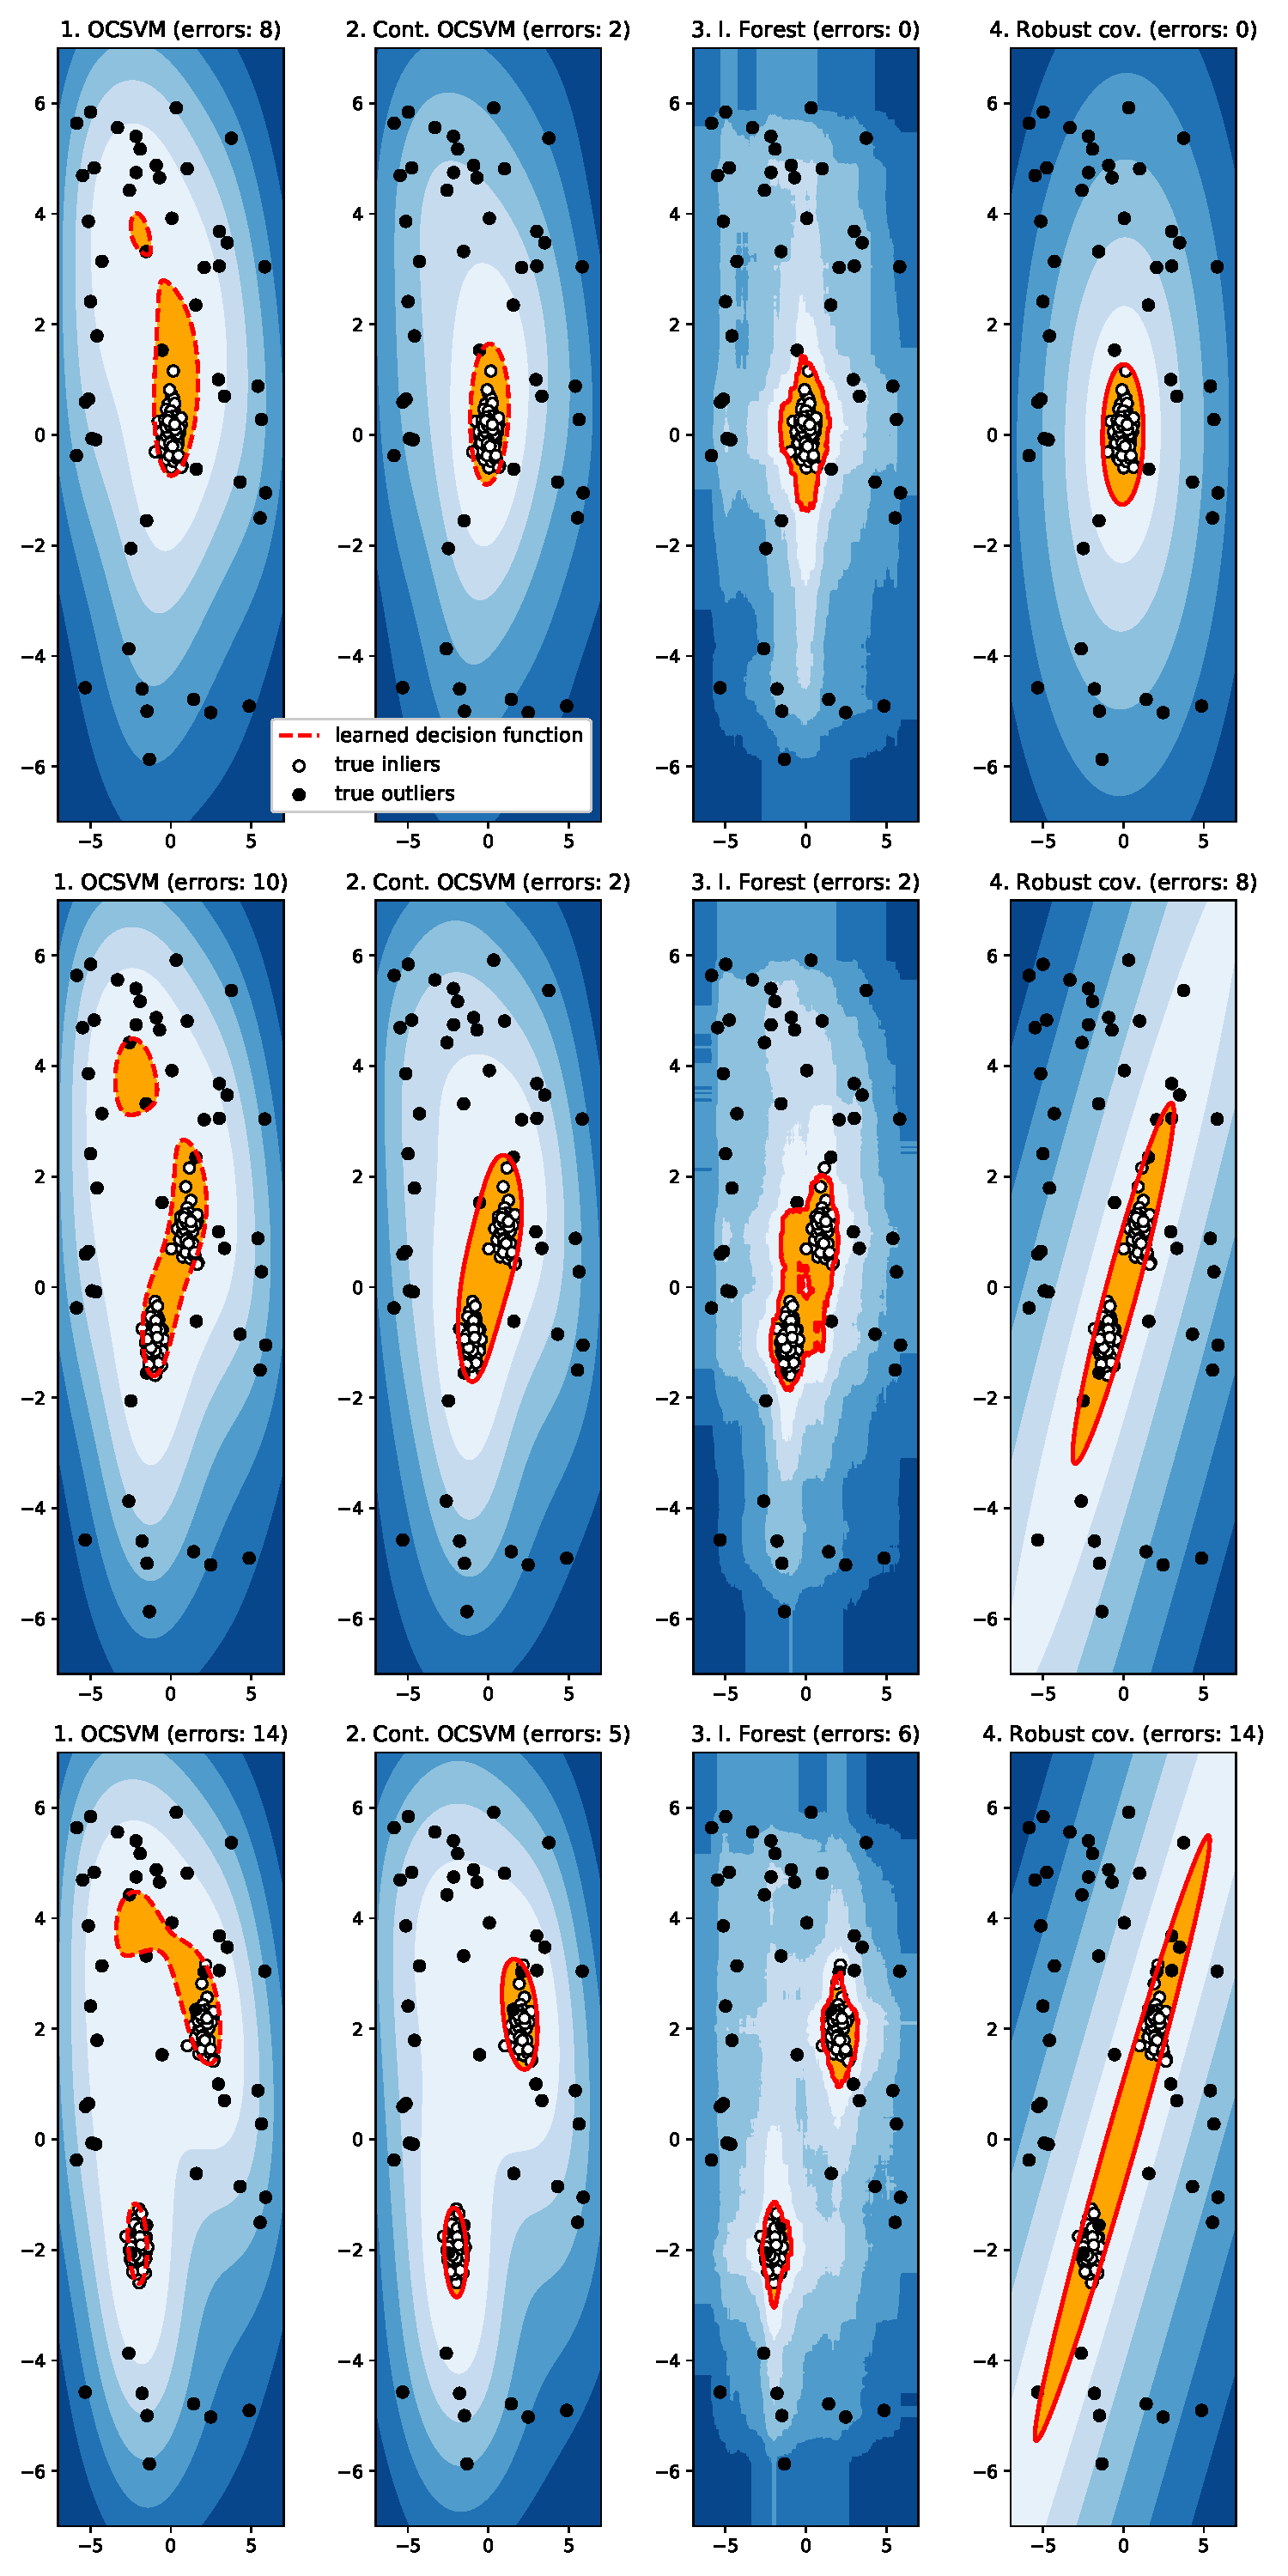
\includegraphics[width=\textwidth]{./gfx/ocsvm.eps}}
    \caption[Continuous OCSVM for outlier detection]{Continuous OCSVM for
    outlier detection. \label{fig:ocsvm_outlier}}
\end{figure}
\paragraph{}
We propose a second experiment in a context of outlier detection. This time
the train set is polluted with outliers. We replicate the example given in
the documentations of Scikit-Learn at
\url{http://scikit-learn.org/stable/auto_examples/covariance/plot_outlier_detection.html}
We compare our method to three other well known outlier detection methods
from the literature: Isolation Forest \citep{Liu2008}, \acs{OCSVM}
\citep{Scholkopf2001} and a Robust Covariance estimator
\citep{campbell1980robust, pedregosa2011scikit} on \cref{fig:ocsvm_outlier}.
Our method achieves the state of the art on this simple example which is
encouraging. However the computation time of our continuous \acs{OCSVM} is
higher than the other methods. It took circa $0.25$ second for the \acs{OCSVM}.
$10$ seconds for our method, $5$ seconds for isolation forest and $0.1$ second
for the Robust covariance estimator. This can be due to the implementation since we used
a (sub-optimal) hand-crafted full gradient descent. Notice that however our
method is able to retrieve all the level sets after training, not only the one
presented in \cref{fig:ocsvm_outlier}.  When one is interested in a specific
level set or range of level set one could sample the $\nu_t$ from another
distribution than the uniform distribution $\mathcal{U}[0, 1]$ to give more
importance to the desired range of level sets.

% %----------------------------------------------------------------------------
% \section{The Nystr\"om method}
% \label{sec:the_nystrom_method}

% %----------------------------------------------------------------------------
% \section{Sub-sampling the data}
% \label{sec:sub_sampling_the_data}

\section{Operalib}
During this Thesis we started the development of a library named \say{Operalib}
implementing various machine learning algorithms based on operator-valued
kernels. We are grateful to Alexandre Gramfort (LTCI, T\'el\'ecom ParisTech)
who served as a technical mentor at the beginning of this software development
and provided many advices.  Operator-valued kernels defines a framework
allowing learning vector/function/structured output.
To install the library it should be as simple as
\begin{lstlisting}[language=bash,caption={Installation of Operalib.}]
pip install operalib
\end{lstlisting}
The library currently features:
\begin{itemize}
    \item Quantile regression \citep{sangnier2016joint},
    \item \acs{ONORMA} \citep{audiffren2013online},
    \item semi-supervised Ridge regression \citep{Brouard2016_jmlr},
    \item some elements of the \acs{ORFF} framework \citep{brault2016random}.
\end{itemize}
The algorithms work for a selection of popular operator-valued kernels such
that the matrix-valued decomposable kernel, the curl-free kernel and the
divergence-free kernel. The library is structured so that it is easy for the
user to define its own operator-valued kernel and plug it to the existing
optimisation algorithms, while keeping efficient computations thanks to the
methodology presented in \cref{subsec:efficient_learning} (\acs{ie} by seeing
operator-valued kernels as operators along with matrix-free solver rather than
plain matrices). We designed the library in order to have a close compatibility
with Scikit-learn. Code and documentation are publicly available at
\url{https://github.com/operalib/operalib}. In a near future we plan to add the
family of works of \citet{Brouard2016_jmlr} around Input Output Kernel
Regression, the  work of \citet{lim2015operator} about the two learning
algorithms defined in \citet{lim2015operator}: a sparse learning of OVK and a
learning algorithm for both kernel and weights with a block coordinate descent
scheme and a proximal gradient method to deal with non-smooth constraints.
Development for modeling time series will be also included. We hope to expand
with more algorithms from various authors of the \acs{OVK} community and
welcome any new contributor!

\chapterend





\chapter{Conlusions}
\label{ch:conclusion}
\include{Parts/Final_words/Conclusions}
